% -*-LaTeX-*-

% The log below is the old log from when RCS was being used in
% conjunction with this.
%
% $Log: master.tex,v $
% Revision 1.7  2010/03/16 00:32:56  stiber
% Final revisions prior to Spring 2010.
%
% Revision 1.6  2007/12/25 18:01:46  stiber
% Final changes for winter 2008.
%
% Revision 1.5  2007/03/20 23:49:49  stiber
% Final cleanup for start of spring 2007.
%
% Revision 1.4  2006/05/13 17:08:46  stiber
% Updated version number for second revision, Spring 2006.
%
% Revision 1.3  2006/03/27 23:32:04  stiber
% Modified for Spring 2006, with corrections and incorporation of
% newer LaTeX packages.
%
% Revision 1.2  2004/03/29 19:46:04  stiber
% Updated for Spring 2004 and new textbook (DSP First).
%
% Revision 1.1  2004/02/19 00:19:10  stiber
% Initial revision
%

\documentclass[12pt]{book}

\newif\ifHtml
\Htmlfalse

\newif\ifPDF
\PDFtrue

\ifHtml
  \PDFfalse
  \usepackage[tex4ht,colorlinks=true,linkcolor=blue,citecolor=blue,urlcolor=blue,pdftitle={Signal Computing: Digital Signals in the Software Domain}]{hyperref}
  \hyperlinkfileprefix{}
\else
  \ifPDF
    \usepackage[pdftex,pdftitle={Signal Computing: Digital Signals in the Software Domain},colorlinks=true,linkcolor=blue,citecolor=blue,urlcolor=blue,bookmarks,bookmarksopen]{hyperref}
    \usepackage{fullpage}
  \else
    \usepackage{hyperref}
    \usepackage{mathptmx,helvet,courier,fullpage}
  \fi
\fi


\usepackage{fullpage,graphicx,algorithmic,multirow,rotating}
%\usepackage{html}
\usepackage[chapter]{algorithm}

% Superscripts outside math mode
\newcommand{\spscript}[2]{\mbox{#1}$^\mathrm{#2}$}

\usepackage{makeidx}
\makeindex

% XMP include for Creative Commons
\usepackage{xmpincl}
\includexmp{metadata}

% Sidebars implemented with picinpar.  Use for defining
% important terms, mentioning important points in the text, indicating 
% the current reading assignment, links to useful resources, etc.
\usepackage{xcolor}
\definecolor{psetback}{HTML}{CFECEC} %html is : light cyan 2
\usepackage{picinpar}
\newcommand{\sidebar}[1]{{\fbox{\parbox{0.4\textwidth}{\footnotesize #1}}}}
%\newcommand{\problemset}[1]{{\fbox{\parbox{0.9\textwidth}{\footnotesize #1}}}}
%\newcommand{\problemset}[1]{{\colorbox{psetback}{{#1}}}}
\newcommand{\problemset}[1]{\vline  {\colorbox{psetback}{{\parbox{0.9\textwidth}{\footnotesize #1}}}}}


% Number figures within the chapter
\renewcommand{\thefigure}{\thechapter.\arabic{figure}}
\renewcommand{\thetable}{\thechapter.\arabic{table}}
\renewcommand{\theequation}{\thechapter-\arabic{equation}}

\setcounter{tocdepth}{2}

% Fancy chapter beginnings
\usepackage[Lenny]{fncychap}

\makeatletter
  \def\@chapapp{}

  \renewcommand{\DOCH}{}

  \renewcommand{\DOTI}[1]{%
    \settowidth{\px}{\CTV\FmTi{#1}\space}
    \addtolength{\px}{5pt}
    \settoheight{\py}{\CTV\FmTi{#1}}
    \addtolength{\py}{1pt}

    \settowidth{\mylen}{\CNoV\thechapter\space\CTV\FmTi{#1}}
    \addtolength{\mylen}{1pt}
    \settowidth{\pxx}{\CNoV\thechapter}
    \addtolength{\pxx}{-1pt}

    \settoheight{\pyy}{\CNoV\thechapter}
    \addtolength{\pyy}{-2pt}
    \setlength{\myhi}{\pyy}
    \addtolength{\myhi}{-1\py}
    \par
    \parbox[b]{\textwidth}{%
    \raggedright%
    \CNoV\thechapter\space\CTV\FmTi{#1}%
    \hskip -\px%
    \rule[\pyy]{\px}{\RW}
    \hskip -5pt%
    \mghrulefill{\RW}%
    \rule{\RW}{\pyy}\par\nobreak%
    \vskip -\baselineskip%
    \vskip -\pyy%
    \hskip \mylen%
    \mghrulefill{\RW}\par\nobreak%
    \vskip \pyy}%
    \vskip 40\p@}

  \renewcommand{\DOTIS}[1]{%
    \settowidth{\px}{\CTV\FmTi{#1}}
    \addtolength{\px}{1pt}
    \settoheight{\py}{\CTV\FmTi{#1}}
    \addtolength{\py}{1pt}

    \settowidth{\mylen}{\CNoV\thechapter\space\CTV\FmTi{#1}}
    \addtolength{\mylen}{1pt}
    \settowidth{\pxx}{\CNoV\thechapter}
    \addtolength{\pxx}{-1pt}

    \settoheight{\pyy}{\CNoV\thechapter}
    \addtolength{\pyy}{-2pt}
    \setlength{\myhi}{\pyy}
    \addtolength{\myhi}{-1\py}
    \par
    \parbox[b]{\textwidth}{%
    \rule[\py]{\RW}{\myhi}%
    \raggedright%
    \CTV\FmTi{#1}%
    \hskip -\px%
    \rule[\pyy]{\px}{\RW}
    \hskip -5pt%
    \mghrulefill{\RW}%
    \rule{\RW}{\pyy}\par\nobreak%
    \vskip -\baselineskip%
    \vskip -\pyy%
    \mghrulefill{\RW}\par\nobreak%
    \vskip \pyy}%
    \vskip 40\p@}
\makeatother

\renewcommand{\topfraction}{0.9} % max fraction of page for floats at top
\renewcommand{\bottomfraction}{0.9}
                 % max fraction of page for floats at bottom
\renewcommand{\textfraction}{0.10} % min fraction of page for text
\renewcommand{\floatpagefraction}{0.8}
                 % min fraction of floatpage that should have floats

% Fancy page headings
\usepackage{fancyhdr}
\setlength{\headheight}{15pt}

\fancyhf{} % clear all header and footer fields
\fancyfoot[L]{Signal Computing}
\fancyfoot[R]{\thepage}
\fancyhead[L]{\slshape\leftmark}
\renewcommand{\headrulewidth}{0.4pt}
\renewcommand{\footrulewidth}{0.4pt}

\fancypagestyle{plain}{%
\fancyhf{} % clear all header and footer fields
\fancyfoot[L]{Signal Computing}
\fancyfoot[R]{\thepage}
\renewcommand{\headrulewidth}{0pt}
\renewcommand{\footrulewidth}{0.4pt}}

\pagestyle{fancy}


% Math and logic
\usepackage{amsmath}
\newcommand{\pred}[1]{\ensuremath{\textit{#1}}}
\newcommand{\const}[1]{\ensuremath{\textsf{#1}}}
\newcommand{\deriv}[2]{\ensuremath{\frac{\mathrm{d} #1}{\mathrm{d} #2}}}
\newcommand{\derivin}[2]{\ensuremath{{\mathrm{d} #1}/{\mathrm{d} #2}}}
\newcommand{\sderiv}[2]{\ensuremath{\frac{\mathrm{d}^{2} #1}{\mathrm{d} #2^{2}}}}
\newcommand{\nderiv}[3]{\ensuremath{\frac{d^{#3} #1}{d #2^{#3}}}}
\newcommand{\pderiv}[2]{\ensuremath{\frac{\partial #1}{\partial #2}}}
\newcommand{\spderiv}[2]{\ensuremath{\frac{\partial^2 #1}{\partial #2^{2}}}}
\newcommand{\pderivin}[2]{\ensuremath{{\partial #1}/{\partial #2}}}
\newcommand{\spderivin}[2]{\ensuremath{{\partial^2 #1}/{\partial #2^{2}}}}
\newcommand{\transpose}{\ensuremath{^{\mathsf{T}}}}
\DeclareMathOperator{\Real}{Re}
\DeclareMathOperator{\Imag}{Im}
\DeclareMathOperator{\sinc}{sinc}

\newcommand{\commentedout}[1]{}

\title{Signal Computing: Digital Signals in the Software Domain}

\author{Michael Stiber \and Bilin Stiber\\ 
{\normalsize University of Washington, Bothell}\\
{\normalsize and}\\
{\normalsize S-Squared Technical Consulting}}

% \date{August 2014}

% \includeonly{ch-fft/fft} % ch-iir/fb-filters} % ch-conv/convolution}
% %
% %intro,ch-physical/physical-signals,ch-computer/computer-signals,ch-fir/filt-intro}

\begin{document}

\begin{titlepage}

\mbox{}\\[0.5in]
\begin{center}
\mbox{}\hrulefill\mbox{}\\[0.25in]
{\Huge Signal Computing:}\\[0.25in]
{\LARGE Digital Signals in the Software Domain}\\[0.25in]
\mbox{}\hrulefill\mbox{}\\[3in]

\mbox{}\hfill
\parbox{1.5in}{\mbox{}}
\parbox{3in}{Fall 2014}\\[0.25in]
\mbox{}\hfill
\parbox{3in}{\raggedright
Prof. Michael Stiber\\
Dr. Bilin Zhang Stiber\\
University of Washington Bothell\\
18115 Campus Way NE\\
Bothell, Washington 98011\\[0.25in]
Eric C. Larson\\
Southern Methodist University\\
Lyle School of Engineering\\
3145 Dyer Street\\
Dallas, TX 75205}
\end{center}

\newpage
\mbox{}\vspace{4in}
\begin{flushright}
Copyright \copyright\ 2002--2014 by Michael and Bilin Stiber and Eric
C. Larson\\[2in]
This work is licensed under the Creative Commons
Attribution-ShareAlike 4.0 International License. To view a copy of
this license, visit
\url{http://creativecommons.org/licenses/by-sa/4.0/}.\\

\includegraphics[height=1.5in]{by-sa}
\end{flushright}

\thispagestyle{empty}

\end{titlepage}

\frontmatter

\tableofcontents
\listoffigures
\listoftables
\listofalgorithms
\markboth{LIST OF ALGORITHMS}{}

% -*-LaTeX-*-

% The log below is the old log from when RCS was being used in
% conjunction with this.
%
% $Log: intro.tex,v $
% Revision 1.5  2007/11/25 02:46:08  stiber
% Revisions for Winter 2008, including updated roadmap and
% typographical conventions.
%
% Revision 1.4  2007/11/25 01:49:33  stiber
% Additional revisions for stand alone book for Spring 2007.
%
% Revision 1.3  2007/03/04 19:34:08  stiber
% Initial revision for stand-alone textbook.
%
% Revision 1.2  2004/03/29 19:46:22  stiber
% Updated for Spring 2004 and new textbook (DSP First).
%
% Revision 1.1  2004/02/19 00:20:54  stiber
% Initial revision
%

\chapter*{Preface}
\addcontentsline{toc}{chapter}{Preface}

\markboth{PREFACE}{}

As computers become ubiquitous, they become more and more embedded not
only in the devices we own and use but in our lives. As a result,
computers become embedded in the physical world, with their primary
purpose being to detect and analyze happenings in our world and to
produce responses that affect that world. As computing professionals,
we need to understand how computers can process information from the
physical world as \emph{digital signals}: multimedia (sound, images,
video) and other measurements (in medical instruments, cars, cell
phones, eyeglasses, etc). This is why we have chosen to coin the
phrase ``Signal Computing''.

Digital signals place great demands on processing power, network
bandwidth, storage capacity, I/O speed, and software design. As a
result, signal computing is a great laboratory for exercising the full
range of knowledge of computer science.

In this book, you will learn how digital signals are captured,
represented, processed, communicated, and stored in computers. The
specific topics we will cover include: physical properties of the
source information (such as sound or images), devices for information
capture (microphones, cameras), digitization, compression, digital
signal representation (JPEG, MPEG), digital signal processing (DSP),
and network communication.  By the end of this book, you should
understand the problems and solutions facing signal computing systems
development in the areas of user interfaces, information retrieval,
data structures and algorithms, and communications.

While there certainly may be many opportunities for you to work in
signal computing, the value of this study extends far beyond. Studying
signal computing and its underlying mathematics directly exercises key
computer science abilities in areas like abstraction and
algorithmics. You will see that this book interleaves mathematical
topics with applications and algorithms. At each step of the way, we
take a representation of digital signals or operations on them that you
are familiar with, reach a concept in which it is awkward or difficult
to use, and then develop an alternative representation that simplifies
matters. This is exactly what computing professionals do in their
careers --- identify that a problem at hand can be represented by some
abstraction with known properties that can be manipulated by
well-understood algorithms. We hope that the journey you take through
the mathematical abstractions here will not only give you an important
set of tools to use later on, but will also help exercise your
fundamental ability to move from one representation to another.

Beyond your own personal professional capabilities, we hope that this
book will also give you a better understanding of the design process
that electrical engineers go through when they design the details of
signal processing systems, such as filters. Even if you do not go on
to build software components that perform signal processing, there is
a good chance that you will work on large systems that have DSP
components. We believe that it will be invaluable for you to
understand the basics of how such DSP components work and what your
electrical engineering colleagues are working on.

\section*{Objectives}
\addcontentsline{toc}{section}{Objectives}

By the end of this book, you should know:

\begin{itemize}
\item What physical signals are like in the ``real'' world and how
  their properties affect how we perceive them.
\item How these signals are \emph{digitized} and the tradeoffs among
  sampling speed, levels of quantization, file size, etc.
\item How to perform simple signal filtering to remove noise,
  emphasize important features, etc.  You should be well-prepared to
  work with electrical engineers in the design of more advanced signal
  processing systems.
\item How to carry out simple time-series analysis techniques to
  analyze frequency and characterize unknown signals.
\item How multimedia file sizes can be reduced by compression, and the
  tradeoffs among compression, processing overhead, and media quality.
\end{itemize}

\section*{Prerequisites}
\addcontentsline{toc}{section}{Prerequisites}

This book covers much of the mathematical foundations for
understanding signals and signal processing; however, it is assumed
that you are familiar with topics such as complex numbers,
trigonometry, derivatives, vectors, the basic idea of integrals,
infinite series, and basic physics (mass, acceleration, force,
etc). Figure~\ref{fg:roadmap} shows these prerequisites in the context
of this book's chapters.

\begin{figure}
\vspace{2in}
\centerline{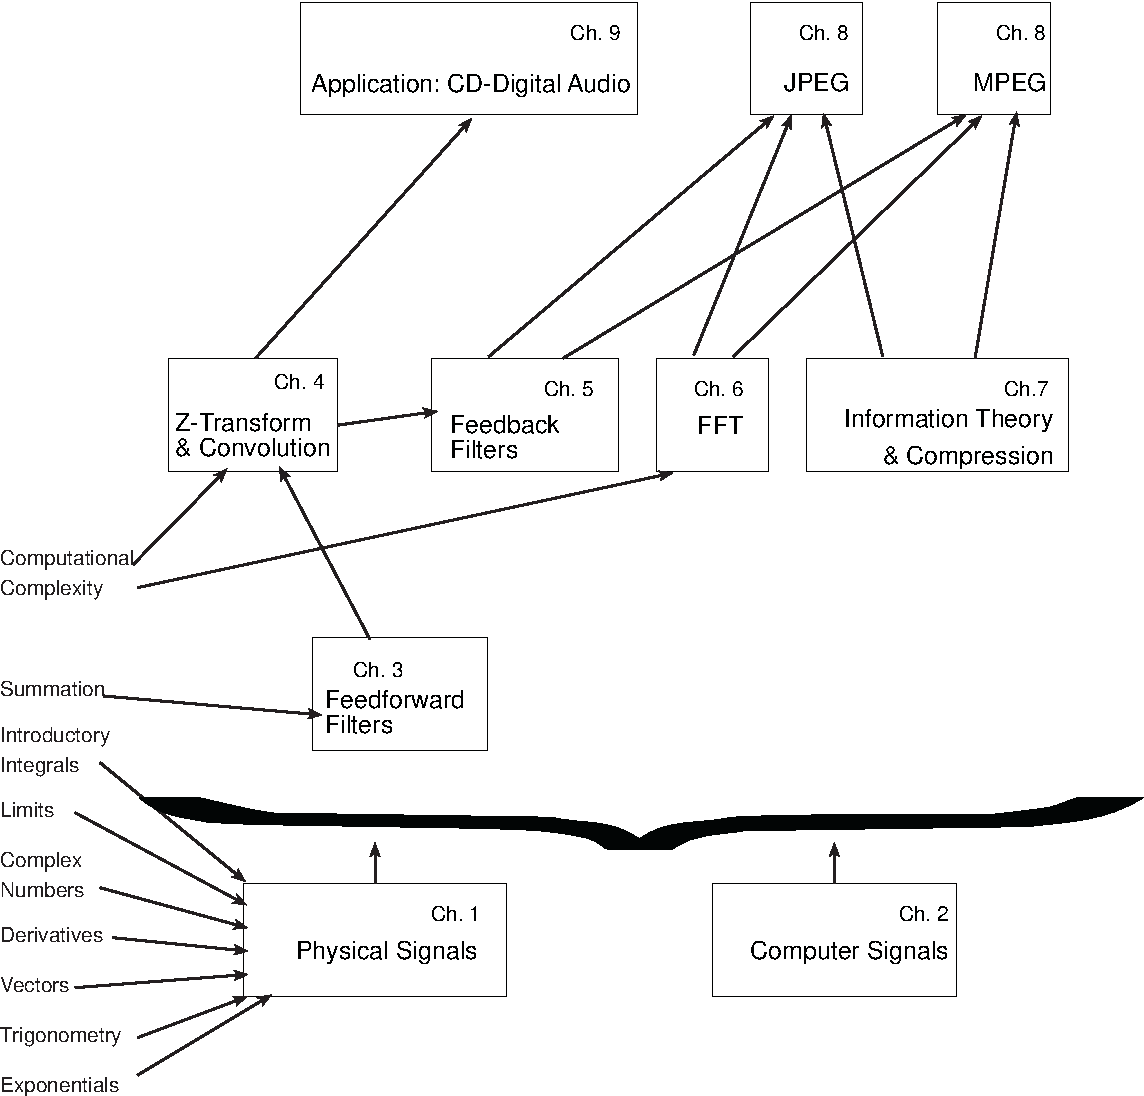
\includegraphics[width=0.9\textwidth]{roadmap}}
\caption[Course conceptual road map]{Course conceptual road
map and background knowledge.\label{fg:roadmap}}
\end{figure}

Figure~\ref{fg:roadmap} also outlines how each chapter's concepts are
used by subsequent ones and what the major themes are. You'll notice
that there's not much in the way of programming indicated. While there
\emph{is} an expectation that you understand the basics of
computational complexity and can understand, appreciate, and analyze
algorithms, this is \emph{not} a programming book. Instead, this is a
book that makes concrete many of the previously abstract mathematical
concepts that you are familiar with. It shows how these concepts
relate to \emph{real} applications that produce tangible changes on
digital signals --- it connects \emph{mathematics} to \emph{bits}.

In the past, this book has been used in a wide range of signal
computing courses, from those that place little emphasis on
programming, to some that required Matlab implementation, and in
others that used C++ or the Java Media Framework.

So, this book and the concepts within can be learned without any
explicit knowledge of low level programming in languages like C, C++,
or Java. Most of the exercises use an online, free tool known as Java
Digital Signal Processing (J-DSP) in order to put together block
diagrams using signal processing techniques.  Most of the problems
involving J-DSP require no background in any type of programming.

However, we also provide problems for students that have varying
levels of programming expertise (for example, you may have already
taken an algorithms or data structures class). If you have some
programming expertise, we provide problems that use simple Java
methods (or functions) in the J-DSP environment.  J-DSP provides a
coding template for you to use, in which you can fill in your own
simple manipulations of variables in the J-DSP environment using Java
and use block diagrams to manipulate signals further.  In this way,
you can focus on the implementation of different algorithms, not the
overhead involved in getting multimedia code working.  If you have
more experience in programming, we provide problems asking you to
write small programs in your choice of a ``lower level'' language
(such as C, C++, or Java).

\section*{About This Book}
\addcontentsline{toc}{section}{About This Book}

This book is divided into nine chapters. Chapters include self-test
questions and review exercises scattered throughout, so we suggest
that you go through all the material sequentially (or, at least, do
the self-test exercises in each section). Answers are provided at the
back of the book. Each chapter concludes with written or programming
assignments and pointers to additional readings.

\index{PDF} If you read the PDF version of this book, you will find
that it is extensively hyper-linked.  This includes links from
exercises to their answers, links to resources on the web, and links
from the table of contents, list of figures, index, etc. to their
respective locations.

Rather than distribute this book via a traditional publishing model,
costing you money and likely netting us very little, we have decided
to make this book freely available for both students and
faculty. Moreover, we have opened the source material for re-use,
updating, and expansion via a Creative Commons Attribution-ShareAlike
4.0 International License. This not only benefits you, it also
benefits us by getting our work into more people's hands.  You can
find the book's home page at
\url{http://faculty.washington.edu/stiber/pubs/Signal-Computing/},
including a pointer to its source material on GitHub. If you find any
errors, make any changes, or find this book useful in your course or
your life, please email us at
\href{mailto:stiber@uw.edu}{stiber@uw.edu}, or send us a pull request.

\subsection*{Typographical Conventions}
\addcontentsline{toc}{section}{Typographical Conventions}

There are no real ``standards'' for much of the notation that is used
in digital signal processing; depending on which textbook you read,
you will encounter different typographical conventions. In this
textbook, we have chosen the following:
\begin{center}
\begin{tabular}{lp{5in}}
  $j$    & $\sqrt{-1}$ \\
  $t$    & continuous time; units typically seconds \\
  $x(t)$ & a real-valued function of continuous time (physical signal) \\
  $f$    & continuous frequency; units cycles/second or Hertz (Hz) \\
  $T$    & an interval of time; often $T=1/f$, meaning the period of a
           signal \\
  $f_0$  & a particular frequency; subscript may vary depending on use \\
  $\omega$ & continuous angular frequency; units radians/second \\
  $\omega_0$ & a particular angular frequency; subscript may vary
               depending on use \\
  $\omega'$ & apparent (continuous angular) frequency, as a result of
                        aliasing \\
  $n$    & discrete time or sample number; dimensionless, but you can
           think of the units as being ``samples'' \\
  $x[n]$ & a function of discrete time; may be real-valued (sampled
           signal) or discrete valued (quantized/digital signal) \\
  $\hat{f}$ & discrete frequency; units cycles/sample \\
  $\hat{f}_0$  & a particular discrete frequency; subscript may vary
                 depending on use \\
  $\hat{\omega}$ & discrete angular frequency; units radians/sample \\
  $\hat{\omega}_0$ & a particular discrete angular frequency; subscript may vary
               depending on use \\
\end{tabular}
\end{center}

\section*{Further Reading}
\addcontentsline{toc}{section}{Further Reading}

An excellent introduction to digital signal processing that is
targeted at beginning electrical engineering students is \textit{DSP
  First: A Multimedia Approach}, by James H McClellan, Ronald
W. Schafer, and Mark A. Yoder (Prentice Hall, 1998).  It is important
to note that that book's target is the design of low-level signal
processing components (i.e., filters) and more generally linear,
time-invariant systems, rather than the role such components play in
overall software systems.


%\newpage

%\pagenumbering{arabic}

\mainmatter

% -*-LaTeX-*-

% The log below is the old log from when RCS was being used in
% conjunction with this.
%
% $Log: physical-signals.tex,v $
% Revision 1.11 2010/5/1 Larson
% Revised wording and figures throughout
%
% Revision 1.10  2007/12/25 18:48:47  stiber
% Corrected error in figure caption.
%
% Revision 1.9  2007/12/25 18:08:22  stiber
% Fixed typo.
%
% Revision 1.8  2007/12/25 17:47:45  stiber
% Some final cosmetic changes.
%
% Revision 1.7  2007/12/01 00:35:49  stiber
% Relatively small revisions from notes from Spring 2007. Ready for more
% extensive rewriting.
%
% Revision 1.6  2007/04/10 19:55:29  stiber
% Minor fixes.
%
% Revision 1.5  2007/03/20 23:51:32  stiber
% Cleaned up LaTeX and minor problems.
%
% Revision 1.4  2007/03/04 20:01:34  stiber
% OK, this time I've taken out all references to material in the old
% textbook, adding in additional figures where necessary.
%
% Revision 1.3  2007/03/04 19:33:24  stiber
% Initial revision for stand-alone textbook.
%
% Revision 1.2  2004/03/29 19:55:18  stiber
% Updated for Spring 2004 and new textbook (DSP First).
%
% Revision 1.1  2004/02/19 00:22:15  stiber
% Initial revision
%

\chapter{Signals in the Physical World}
\label{ch:physical-signals}

This chapter introduces the fundamental concepts of multimedia from an
``outside the computer'' perspective. We define the term
``multimedia,'' discuss why it is an important issue, how multimedia
signals (sound, images) are generated in the ``real world'' (by both
natural and artificial means) and how we perceive them. We also
introduce a set of convenient mathematical tools for describing
signals. When you are done with this chapter, we hope you will
appreciate the complexity and importance of multimedia communications
and will be eager to see how signals can be processed by computer.

\section{Multimedia and Sensation}

\begin{quote}
``What can give us surer knowledge than our senses? With what else can
  we better distinguish the true from the false?'' \textit{Lucretius}
\end{quote}

Humans, like any other organisms, depend on their senses to provide
information critical to their development and survival. Over time,
life has evolved sophisticated systems for capturing information about
the physical world. The first senses were almost certainly chemical
--- what we would call taste or smell. These senses have a number of
drawbacks: they typically require close physical presence or even
direct contact, they have poor temporal resolution (you can tell that
someone was cooking onions, but not \emph{when}), and they have poor
spatial resolution (from where is that bad smell coming?). Other
senses --- hearing, seeing, electrical senses that fish have, magnetic
senses that birds have --- allow us to gather information remotely
from the information source.

Given all this, it is perhaps not surprising that people find computer
systems difficult to use, uninspiring, or even objects of
distaste. Computers by and large produce a very impoverished set of
stimuli, composed almost entirely of patterns of light that we must
interpret as text (when people use devices that provide a richer
experience, such as tablets or smartphones, they often mentally
categorize them just that way: as \emph{devices}, not
\emph{computers}). It is only fairly recently that computers have done
much more than this, as processing power and hardware speed has
enabled \emph{multi}media capabilities (though these are almost always
used to imitate other appliances, like televisions, telephones, photo
albums, etc., rather than to produce new things). The goal of making
computers more ``human friendly,'' then, depends on our ability to
process multimedia information digitally, and to do so in a
\emph{useful} fashion. But what is useful? The answer to this question
depends on the user, and central to the user is how his or her sensory
system works.

\section{Sensation and Perception}

\index{perception!visual|(}
\index{perception!visual!color constancy}
\index{perception!visual!cone}
\index{perception!visual!luminance}
\index{perception!visual!photoreceptor}
\index{perception!visual!retina}
\index{perception!visual!rod}
\index{perception!visual!trichromatic}
\begin{window}[0,r,%
\sidebar{\textbf{Important Terms:}\\
\begin{description}
\item[color constancy] our ability to perceive object color
  independent of light source qualities.
\item[cone] a \emph{photoreceptor} that supports color vision.
\item[luminance] measure of visible light strength.
\item[photoreceptors] sensory cells in the \emph{retina}.
\item[retina] Layer of sensory and other neurons at the back of the
 eye.
\item[rod] a \emph{photoreceptor} that supports low-light-level
 vision.
\item[trichromatic vision] construction of color sensation from
  measurement of three primary colors.
\end{description}},{}]
Regardless of the sensory \emph{modality}, all senses have one thing
in common: they are composed of cells which are responsive to some
property of the physical world and whose responses are
\emph{interpreted} by a nervous system to \emph{construct a model} of
the world. In other words, the world does not ``look'' like our
perception.  Our perception is a \emph{construct}; an interpretation.
\index{perception!as a construct}

For example, consider sight. Our environment is constantly bathed in a
sea of radiation, which we can think of as sinusoidal waves of varying
wavelength, ranging from very long (radio waves) to very short
(X-rays, gamma rays), and amplitude.  Some of this radiation is
absorbed by objects and some is reflected, depending on the objects'
properties.  The ``goal'' of our visual system is \emph{not} to
provide us with information about reflected energy.  Our visual system
has evolved in tandem with the rest of our nervous system for the
purpose of extracting useful information about objects' properties
based on reflected radiation.  In this respect, it is much like a
remote-sensing satellite and ground data analysis system: we want to
know about crop conditions, we gather reflected light data at a number
of wavelengths, and then we analyze the data to produce a report on
crop conditions. We don't really care about the reflected light; it is
merely a means to an end.
\end{window}

Likewise, when we ``see'' a chair, what we perceive is no more a chair
than the word ``chair'' is a chair. It is an \emph{internal
representation} of a chair --- a useful representation, which can
allow us to recognize the object's purpose, location, size,
composition, etc., but a representation nonetheless. What we perceive
about the world is at least as much a psychological issue as a data
acquisition one. For brevity's sake, however, we will confine ourselves in
this section to discuss the basics of ``low-level'' sensory organs,
rather than high-level perceptual issues.

Our eyes are made up of an optical system and a sensory system.  The
sensory system --- the \emph{retina} --- is composed of a number of
different kind of nerve cells arranged in well-structured layers. We
won't go into the details of the eye's structure, but instead
concentrate on one class of cells: the \emph{photoreceptors}.

Photoreceptors are specialized cells that contain pigments that absorb
light and respond electrically (to make a complex matter simple).
Each pigment is responsive to a fairly narrow range of light
wavelengths, and in total, we can see a range of \emph{visible light}
\index{perception!visual!visible light}
\index{visible light}
\index{spectrum!visible}
with wavelengths between roughly 400 nanometers ($400 \times 10^{-9}$
meters) and 700nm --- this from an electromagnetic spectrum that covers
$1 \times 10^{-6}$nm to thousands of kilometers.
\index{spectrum!electromagnetic}

Our eyes have photoreceptors specialized for color vision at high
(daytime) light levels (called \emph{cones}) and photoreceptors
\index{perception!visual!cone}
\index{perception!visual!photoreceptor}
specialized for low (nighttime) light levels (called \emph{rods}).
\index{perception!visual!rod}
There are three cone types, each with a pigment sensitive to a
different range of light wavelengths.  These are usually termed red,
green, and blue, though the correspondences to these colors is not
exact. The fact that our visual system combines measurements of three
``colors'' of light to form our perception of color is known as
\emph{trichromatic vision}.
\index{perception!visual!trichromatic}

\index{perception!visual!color|(}
We do \emph{not} experience light as a set of intensity
(\emph{luminance}) measurements at a variety of light wavelengths,
however.  We experience light as having \emph{color}. Color is a
complex psychological issue, and it is still not understood exactly
how this is achieved. A simple proof-by-contradiction of the idea that
the color we see is the ``color'' of the light hitting our eyes is the
observation that we see objects as having the same color under a wide
range of lighting conditions (morning sunlight, afternoon sunlight,
incandescent lighting). In each of these circumstances, the light
reflected from the objects around us is very different because the
illuminating light is different.  The fact that our perception of
color is more characteristic of the objects' surface properties than
the illuminating light is called \emph{color constancy}. Again, our
perceptual system acts to give us information about \emph{things}, not
measurements of incoming data.
\index{perception!visual!color|)}
\index{perception!visual|)}

\index{perception!auditory|(}
Similar observations can be made of our sense of hearing. Sound is
made of moving waves of varying air pressure, in a manner analogous to
ripples on a pond. These waves are eventually transduced by auditory
neurons, each sensitive to a relatively small range of frequencies
(low pitched sounds, high pitched sounds --- the full range of audible
sounds).  Yet, we do not perceive a set of signal strengths, just as
we don't for light.
\index{perception!auditory|)}

Even more extraordinarily, though our sensors for sound and light are
distinct and very different, we don't have separate sensations of
hearing and vision.  Instead, we perceive the world as a unified
whole, with sound and appearance being properties of the objects
around us. Our brains \emph{fuse} the incoming sensory stimuli and
\emph{construct} a \emph{synthetic} experience.
\index{perception!multimodal fusion}

All of the foregoing is of course a great simplification of how these
systems actually work.  However, these issues have great impact on the
design of computer multimedia systems, because the main point of such
systems is delivering a particular user experience. In the following
sections, we will outline first how computer systems can generate
images, then delve deeper into how we can develop a more precise,
mathematical view of sound. This mathematical view will be essential
to our understanding of computer representation and manipulation of
multimedia information.

When we eventually want to represent physical signals in the computer,
perception of the signals will play an even more vital design
role. For instance the sensors we use to capture light and sound are
not nearly as advanced as the human eye or human ear. They contain
various forms of noise that corrupt the \emph{integrity} of the
signal. The difference between how we perceive \emph{physical signals}
and how we perceive signals that have been \emph{captured by different
  sensors} will be of great importance to us. We will return to this
concept later on.

\section{Computer Video Displays}

\begin{figure}
\centerline{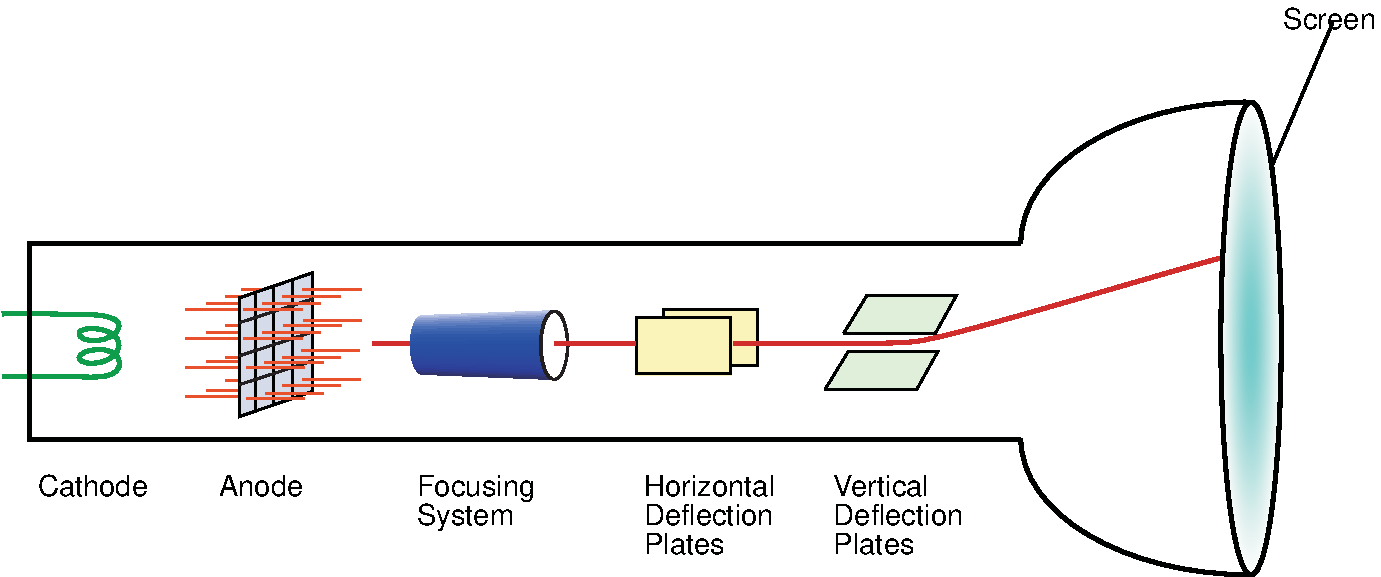
\includegraphics[width=\textwidth]{ch-physical/crt}}
\caption{Schematic diagram of a CRT.\label{fg:crt}}
\end{figure}

The two most prevalent computer displays are \emph{cathode ray tubes}
(CRTs) and \emph{liquid crystal displays} (LCDs); we'll just discuss
\index{CRT|(}
\index{LCD}
CRTs here (while they are becoming rarities, their operation is more
accessible for our purposes here). A simplified CRT is sketched in
figure~\ref{fg:crt}. It is
composed of an \emph{electron gun}, which generates \emph{cathode
\index{CRT!electron gun|(}
rays} (aka, ``electrons''). In this gun, a metal cathode is heated to
\index{CRT!cathode}
\index{CRT!cathode rays}
cause electrons to ``boil off;'' they are accelerated toward the
screen by a positively-charged anode (or possibly by charging the
\index{CRT!anode}
screen itself), which attracts the negatively-charged electrons. In
between the anode and the cathode is a negatively-charged control
grid. By varying the charge on the control grid, the intensity of the
beam can be varied in a manner analogous to the way that a faucet
valve controls the flow of water.

After leaving the electron gun, the flow of elecrons is focused into a
narrow beam by an electrostatic or magnetic focusing system. The
focused beam then passes by deflection plates, which can ``steer'' the
beam magnetically to hit any part of the screen.
\index{CRT!electron gun|)}

The screen itself is coated with one (for B\&W) or more (for color)
\emph{phosphors}: chemicals which glow (emit visible light) when struck
\index{CRT!phosphor}
by electrons. Different phosphors emit different light wavelengths,
and so multiple phosphors can be used to produce the perception of
color images (typically by combining red, green, and blue
phosphors). Another property of phosphors is \emph{persistence}: how
long it will glow after an impinging electron beam is removed. Low
persistence phosphors will require that the screen image be
\emph{refreshed} more often (by repainting the screen with the
electron beam); otherwise, the display will flicker. On the other
hand, a high persistence phosphor will glow longer, and so will
produce blurry moving images.

\begin{figure}
\centerline{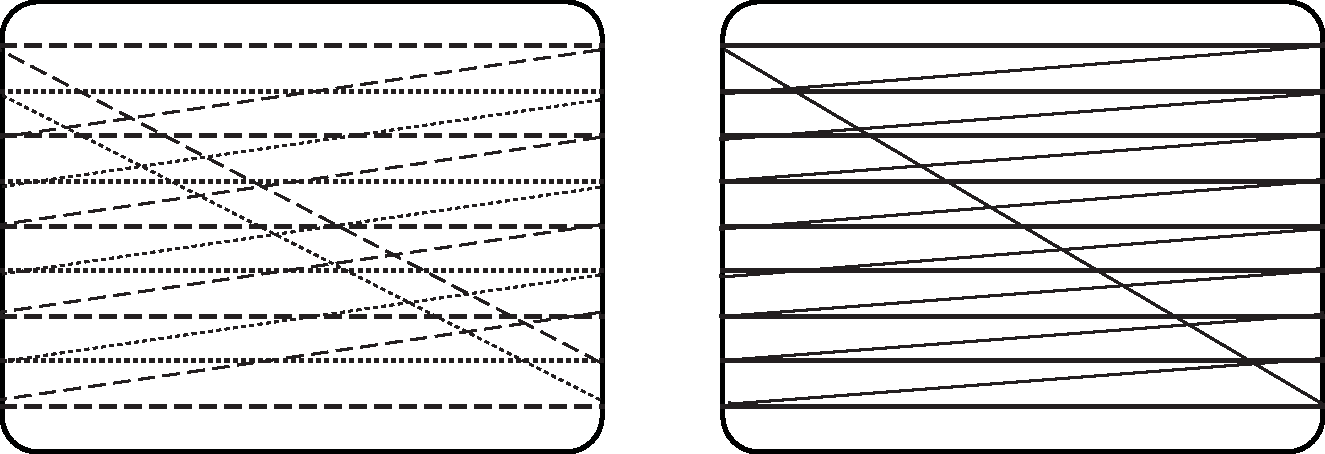
\includegraphics[width=\textwidth]{ch-physical/raster}}
\caption[Interlaced and non-interlaced raster 
  scanning]{Interlaced (left) and non-interlaced (right) raster
  scanning.\label{fg:raster}}
\end{figure}

\index{CRT!raster scanning|(}
So, how can we ``paint'' a two-dimensional image with an electron beam
that only creates a single spot on the screen? We do this by
\emph{raster scanning} the beam, as shown in
figure~\ref{fg:raster}. The horizontal and vertical deflection systems
work in concert with the control grid to move the beam across the
screen while varying its intensity. When the beam moves across the
screen horizontally, its intensity is varied in proportion to the
desired light intensity. While the deflection system resets to the
beginning of the next horizontal line, the beam is turned off. This is
called \emph{horizontal retrace}.

Subsequent lines are painted on the display in a similar manner until
the bottom of the screen is reached --- this is one \emph{frame}. At
that point, the beam is turned off and the deflection system resets
itself to the beginning of the top screen line; a process called
\emph{vertical retrace}.

For computer displays, a frame is usually displayed in between 1/60
and 1/80 of a second (though some displays have higher refresh
rates). Typically, such displays are non-interlaced
\index{CRT!raster scanning!non-interlaced}
(figure~\ref{fg:raster}, right). Analog televisions, on the other
hand, have interlaced displays (left). Interlaced raster scanning
\index{CRT!raster scanning!interlaced}
involves painting all of the odd scan lines in about 1/60 of a second,
then a vertical retrace, and a painting of the even lines.  This
allows the TV 1/30 of a second to display an entire frame and yet
still presents a flicker-free image (because every other line is
refreshed every 1/60 of a second).
\index{CRT!raster scanning|)}

\index{CRT!color|(}
This explains how a greyscale display works. But, what about color? A
color display requires three different phosphors, usually considered
to be red, green, and blue (RGB). In color monitors, three electron
guns are used --- one dedicated to each color. The guns are aligned so
that their beams strike slightly different spots on the screen. The
three phosphors are laid down in a pattern so that each color gun's
beam will hit the appropriate phosphor for each pixel. By varying the
intensity of each beam appropriately, control of the relative mix of
the three primary colors (and thus the perceived color) and the
overall brightness is possible.
\index{CRT!color|)}
\index{CRT|)}

\section{Multimedia System Operation}

\index{multimedia systems!basic functions|(}
Multimedia systems need to support four basic functions:

\begin{enumerate}
\item They must support appropriate user \emph{perception} of the
media --- provide output media and represent (code) media in such a
way that the output seems natural.
\item They must be able to \emph{retain} media --- store it and
provide efficient access (perhaps in a database).
\item They should allow users to \emph{reason} about media
information.  If the goal is greater than a digital television or
radio, then users must be able to manipulate the media.
\item They must be capable of \emph{transmitting} media between
machines. This can have significant impact on networking, resource
allocation, and synchronization of activity across geographically
distributed computer systems.
\end{enumerate}

\index{multimedia systems!computing requirements}
All of these place a high demand on computer power. For example, let's
assume that we encode audio information as 8 bits per sample at 8000
samples per second (this would be considered very low quality). How
many bits per second is that (answer in~\ref{sc:ch1ex}
\#\ref{it:ch1ex1})? Perhaps that doesn't sound too bad, so let's
consider video. Let's say we encode each frame in a video stream as
1000x1000 pixels, 24 bits/pixel, and 30 frames/second.  How many bits
per second is that (answer in~\ref{sc:ch1ex}
\#\ref{it:ch1ex2})?
Even if we were to achieve an extremely high compression ratio of
1/500, this would still mean more than 1 million bits/second.

On the one hand, we can attack this problem through faster
hardware. But you should be well aware by this time that the
difference between a good algorithm and a bad one can be the
difference between an application which places very little load on a
modest CPU and one which takes all the power of a supercomputer. That
is what we will be focusing on here: developing the mathematical
underpinning for developing efficient multimedia signal processing
algorithms.
\index{multimedia systems!basic functions|)}

\section{Vibrations and Sound}

For much of this book, we will focus on sound when talking about
signals. The reason we do this is that sound is simpler than
video. Sound is a one-dimensional function of time (amplitude versus
time), while video is at least a three-dimensional function of time
(intensity at each $x$ and $y$ pixel location as a function of time
for greyscale; R, G, B values at each $x$ and $y$ pixel location as a
function of time for color).

Sound is carried by pressure waves in the air. These pressure waves can be generated by a variety of different sources. Ideally, the human ear responds to anything that vibrates between about 20 Hz and 20 kHz. A stereo speaker in a home theater system generates sound by vibrating a flexible cone. The human vocal tract generates sound by rapidly opening and closing a muscle called the glottis as air passes through it from the lungs. Musical instruments resonate at specific frequencies depending on the width and length of strings or pipes.

In nature, sound is the result of a chaotic mix of events. It may at first seem surprising, then, that most sounds occurring in nature \emph{repeat} (usually hundreds or thousands of times per second). Figure \ref{fg:periodicexample} shows graphs of sounds generated from a tuning fork and the vocal tract (the sound `a' like in bat). In each case notice that the some portion of the wave repeats; repeating signals are commonly called \emph{periodic}. This phenomenon has spurred scientists and mathematicians to develop standard means of representing periodic signals. 
\begin{figure}
\centerline{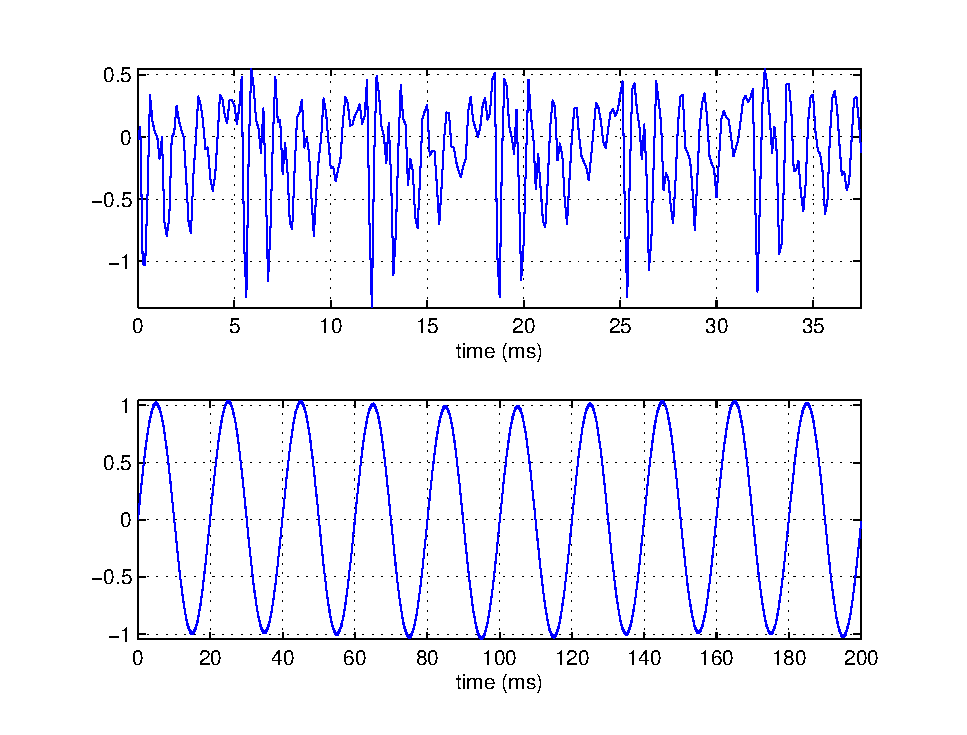
\includegraphics[width=\textwidth]{ch-physical/periodic-examples}}
\caption[Real periodic signals]{Real periodic signals. Top: human speech of the vowel `a' as in `bat.' Bottom: ringing of a tuning fork. \label{fg:periodicexample}}
\end{figure}

As we will see, it turns out that any periodic signal can be
represented as a weighted sum of \emph{harmonically} \index{harmonics}
related sines and cosines (sinusoids at frequencies that are integer
multiples of each other). If a periodic signal has a period of $T_0$
(where period is merely the reciprocal of frequency, so $T_0 =
1/f_0$), it can be represented by a weighted sum of sinusoids at
harmonics of $T_0$, namely sinusoids with periods of $T_0$,
$\frac{1}{2}T_0$, $\frac{1}{3}T_0$, $\frac{1}{4}T_0$, $\cdots$. This
is potentially very powerful! It means that if we know the period of
any repeating function, we can represent it by a discrete set of
weights (one weight for each harmonic).

Each weight tells us exactly how much to multiply by each harmonic, and thus, how much of a certain frequency is present in a given signal. By graphing the weights of each harmonic versus the frequency, we can analyze the frequency content of the signal. This is commonly known as the Fourier Series (we will discuss this later). 

The reason sines and cosines occur so often in nature is due to the physics of the way objects vibrate. When an object is acted on by a force, the way the object moves (its displacement) is a function of its velocity and acceleration. When solving for the exact displacement equation, $x(t)$, we often end up with an equation of the form,

\begin{equation}
\sderiv{x(t)}{t} = -C x(t) \label{eq:diffeq1}
\end{equation}
\index{differential equations}
where C is some constant and $\sderiv{x(t)}{t} $ is the acceleration of the object. This kind of equation --- which relates a derivative of
something to itself --- is called a \emph{differential equation}. We
bet you didn't know they were that simple! To \emph{solve} a
differential equation, we look for a function, $x(t)$, that will satisfy the equation. This is analogous to
solving an algebraic equation, where we look for a number that
can be substituted for a given variable.  
The only difference is that numbers fall along a
one-dimensional number line (unless we're talking about complex
numbers), while there is no such neat number line for all possible functions.  So, we
need to find a function, $x(t)$, whose second derivative is proportional
to itself. Can you think of one or two (answer in~\ref{sc:ch1ex}
\#\ref{it:ch1ex3})?

Luckily, people have been working with functions and differential
equations for a while, and so finding such functions is not
difficult.  For example, consider sinusoids.  The first and second
derivatives of $\sin\omega t$ are:

\begin{gather}
\deriv{}{t} \sin\omega t = \omega\cos\omega t\\
\sderiv{}{t} \sin\omega t = \deriv{}{t} \omega\cos\omega t\
   = -\omega^2 \sin\omega t
\end{gather}

Therefore, differential equation~(\ref{eq:diffeq1}) describes
\emph{simple harmonic motion}: sinusoidal vibration of a simple object. 
Sinusoids occur naturally in the real world when an object is acted on by a force! More complicated forces and objects result in more complicated differential equations, but they almost always involve sines and cosines.

%\index{tuning fork|(}
%As I said earlier, sound is carried by pressure waves in the air. such
%pressure waves can be generated by vibrating a physical object.  For
%example, a speaker generates sound by vibrating a flexible cone. Let's
%start with a simple vibrating system: a tuning fork producing a pure
%tone. And, to make things even simpler, we'll consider only a
%single-tine fork (a tuning chopstick?).
%
%\begin{figure}
%\centerline{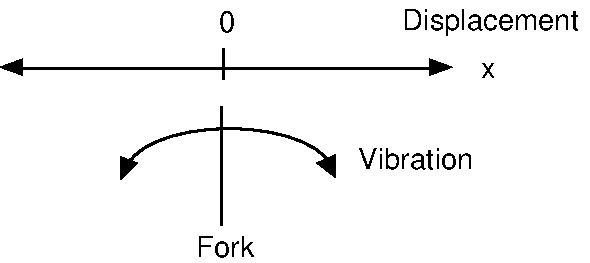
\includegraphics[width=\textwidth]{ch-physical/tuningfork}}
%\caption{Vibration of an idealized tuning fork.\label{fg:tuningfork}}
%\end{figure}
%
%There are three concepts central to our understanding of how the
%idealized tuning fork in figure~\ref{fg:tuningfork} vibrates:
%\begin{description}
%\item[deformation] The fork is assumed to be fixed at one end and free
%  at the other, which swings back and forth as the fork vibrates. So,
%  the material the fork is made of is \emph{bent} as the end swings.
%\item[inertia] An object (such as the end of the vibrating fork)
%  exerts a force proportional to its mass when one tries to accelerate
%  or decelerate it. We can write the equation for this force as $F_i =
%  ma$, where $F_i$ is the inertial force, $m$ is the object's mass,
%  and $a$ is the acceleration.
%\item[elastic forces] Deforming the fork requires application of
%  force.  In the case of our tuning fork, the force results from its
%  inertia. Let's make the simplifying assumption that the fork acts
%  like an ideal spring. That means that as the fork is bent from the
%  vertical ($x=0$ in the figure), the elastic force increases
%  proportionately to $x$. So, $F_e = -kx$, where $F_e$ is the elastic
%  force, $k$ is the spring constant (how stiff the fork is), and the
%  minus sign indicates that the direction of the force is opposite the
%  directio of the bend (always towards $x=0$).
%\end{description}

%So, we pull the fork and release it.  The elastic force results in an
%acceleration towards $x=0$ and the tip speed builds up.  When the tip
%passes $x=0$, the elastic force decelerates the tip, it stops, and the
%whole thing repeats. If we ignore troublesome issues like air
%resistance that would slow down the vibration, then $F_i = F_e$.
%Solving for $a$ we obtain:
%
%\begin{align}
%F_i = ma &= -kx = F_e \\
%a &= -\frac{k}{m} x
%\end{align}
%
%Acceleration is the change in velocity over time, or its derivative,
%$a = \mathrm{d}v/\mathrm{d}t$; velocity in turn is the derivative of
%distance, $v = \mathrm{d}x/\mathrm{d}t$. So, acceleration is the second
%derivative of $x$:
%
%\begin{equation}
%a = \deriv{v}{t} = \sderiv{x}{t} = -\frac{k}{m} x \label{eq:tuningfork}
%\end{equation}
%
%\index{differential equations}
%As an aside, this kind of equation --- which relates a derivative of
%something to itself --- is called a \emph{differential equation}. I'll
%bet you didn't know they were that simple! To \emph{solve} a
%differential equation, we look for a function of $x$ that, when
%plugged in for $x$, will satisfy the equation. This is analogous to
%solving an algebraic equation, where we look for a number that
%satisfies.  The only difference is that numbers fall along a
%one-dimensional number line (unless we're talking about complex
%numbers), while there is no such neat ordering of functions.  So, we
%need to find a function of $x$ whose second derivative is proportional
%to itself. Can you think of one or two (answer in~\ref{sc:ch1ex}
%\#\ref{it:ch1ex3})?
%
%Luckily, people have been working with functions and differential
%equations for a while, and so finding such functions is not
%difficult.  For example, consider sinusoids.  The first and second
%derivatives of $\sin\omega t$ are:
%
%\begin{gather}
%\deriv{}{t} \sin\omega t = \omega\cos\omega t\\
%\sderiv{}{t} \sin\omega t = \deriv{}{t} \omega\cos\omega t\
%   = -\omega^2 \sin\omega t
%\end{gather}
%
%Therefore, differential equation~(\ref{eq:tuningfork}) describes
%\emph{simple harmonic motion}: sinusoidal vibration of the tuning
%fork's tip.
%\index{tuning fork|)}
%
%\subsection*{Self-Test Exercises}
%
%See~\ref{sc:ch1ex} \#\ref{it:ch1ex4}--\ref{it:ch1ex5} for answers.
%
%\begin{enumerate}
%\item Solve for $\omega$ in terms of $k$ and $m$.
%\item Fork stiffness ($k$) clearly affects vibration frequency. As the
%  fork get stiffer ($k$ increases), does the vibration frequency go up
%  or down?
%\end{enumerate}

\subsection*{Sinusoid Phase}

Because sines and cosines are so powerful it is necessary to represent them as neatly and compactly as possible. Above we saw why $\sin\omega t$ occurs naturally. The same argument can be used for $\cos\omega t$.  In fact, cosine is
just a delayed version of sine, as $\cos\omega t = \sin(\omega t +
\pi/2)$.  So, a more general solution to~(\ref{eq:diffeq1}) would
be:
\begin{equation}
x(t) = \sin(\omega t + \phi) \label{eq:gensine}
\end{equation}

\index{phase!of a sinusoid}
In~(\ref{eq:gensine}), $\phi$ is called the sinusoid's \emph{phase}:
the time closest to $t=0$ when $x(t)=0$ (for the case of a sine; it
would be when $x(t)=1$ for a cosine). Depending on \emph{when} an object
starts vibrating (and our time reference; the time that we call $t=0$),
we will get sinusoids of differing phase.

Let's use tuning forks as an example. 
What would happen if we hit two identical tuning forks but at
different times?  They would vibrate at the same frequency, but would
have differing phases and amplitudes (loudnesses).  If the two forks
were close together, we would hear the sum of their tones. What would
that sum be (answer in~\ref{sc:ch1ex} \#\ref{it:ch1ex6})? Simplifying
this sum would be involved; we would have to remember all sorts of
trigonometric identities and then crank out the algebra. Luckily, we
can come up with another representation of a sinusoid which simplifies
this problem considerably. In fact, much of the new math we will cover
in this course is primarily focused on making the paper-and-pencil
work easier.

\section{Phasors}

\begin{figure}
\centerline{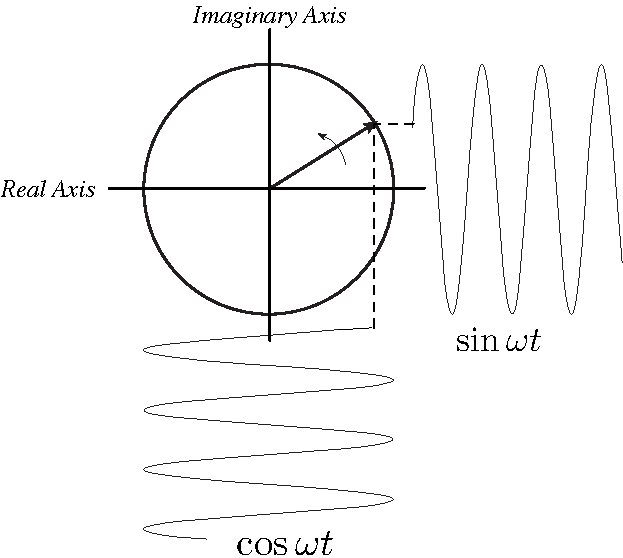
\includegraphics[width=0.5\textwidth]{ch-physical/phasor-components}}
\caption{Components of a phasor are sinusoids.\label{fg:phasor-components}}
\end{figure}

Instead of thinking of a sinusoid as a function which oscillates up
and down, let's think of it as something that goes round and round: a
rotating vector of length $a$ (where $a$ is the sinusoid's
amplitude). Think of this vector rotating around the origin of the
$x$-$y$ plane.  At any point in time, the vector makes an angle
$\theta(t)$ with the positive $x$ axis. The phase, $\phi$, is defined
as $\phi = \theta(0)$ (i.e., the angle that the vector makes with the
$x$-axis at $t=0$).  As figure~\ref{fg:phasor-components} shows, the
$x$ and $y$ \emph{components} of the vector as it moves
counterclockwise are cosine and sine functions.

If we have two vectors $\mathbf{u}$ and $\mathbf{v}$, we can add them
by adding their components.  This is done graphically in
figure~\ref{fg:vector-sum} by placing the ``tail'' of one vector on
the ``head'' of the other. The sum $\mathbf{u}+\mathbf{v}$ is the
vector from the origin to the ``head'' of the second vector. Of
course, that's just the sum at one point in time. What does
$\mathbf{u}+\mathbf{v}$ look like if $\mathbf{u}$ and $\mathbf{v}$ are
rotating at the same rate (answer in~\ref{sc:ch1ex} \#\ref{it:ch1ex7})?

\begin{figure}
\centerline{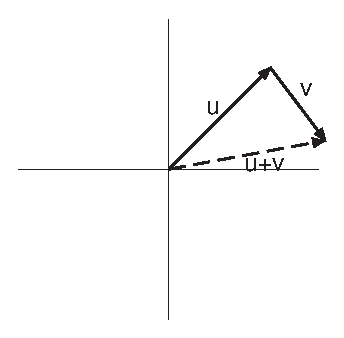
\includegraphics[width=0.5\textwidth]{ch-physical/vector-sum}}
\caption{Graphical summation of vectors.\label{fg:vector-sum}}
\end{figure}

\subsection*{Complex Exponential Representation}

While we used the $x$ and $y$ axes above as frames of reference (for
considering components --- sine and cosine --- of the vector), we
didn't actually define what the plane was. Let's imagine that our
rotating vectors are in the \emph{complex} plane, where $x$ is the
real axis and $y$ is the imaginary axis.  At any point in time, the
location of a vector is therefore a complex number: \index{complex
  numbers|(emph}

\begin{equation}
\mathbf{v} = x + j y \label{eq:complexrect}
\end{equation}

\index{j ($\sqrt{-1}$)}
\index{i|see{j}}
We use $j$ here for $\sqrt{-1}$, rather than $i$ as you've probably
seen before, to adhere to the convention used by electrical engineers
(who use $i$ for current). This notation allows us to represent vectors in the complex plane as complex numbers.

\index{complex numbers!rectangular form}
\index{complex numbers!polar form}
\index{complex numbers!magnitude|see{complex numbers, polar form}}
\index{complex numbers!angle|see{complex numbers, polar form}}
Note that equation \ref{eq:complexrect} is the \emph{rectangular} representation of complex
numbers; we can also represent them in polar form (magnitude and
angle), written as $R\angle\theta$. 


\problemset{
\subsubsection*{Review Exercises: Complex Numbers}
\begin{enumerate}
\item What is the sum of the two complex numbers $x + jy$ and $v +
  jw$ (answer in~\ref{sc:ch1ex} \#\ref{it:ch1excn1})?
\item What is the
product of the two complex numbers $x + jy$ and $v +
  jw$ (answer in~\ref{sc:ch1ex} \#\ref{it:ch1excn2})?
\item Convert the complex number $z = x + jy$ to polar form,
  $R\angle\theta$ (answer in~\ref{sc:ch1ex} \#\ref{it:ch1excn3}).
\item Multiply the two polar-form complex numbers $R_1\angle\theta_1$ and
  $R_2\angle\theta_2$ (answer in~\ref{sc:ch1ex} \#\ref{it:ch1excn4}).
\end{enumerate}
\index{complex numbers|)}}

So, we have an easier-to-manipulate representation of a vector
\emph{at one point in time}. But, we want to represent a \emph{rotating}
vector.  Let's talk about a ``standard'' sinusoid --- one with unit
amplitude --- and let's call this $E(\theta)$.  We know from our first
discussion of the rotating vector representation that cosine and
sine are the $x$ and $y$ axis projections of the vector, so let's
rewrite our rectangular form in the complex plane as:

\begin{equation}
E(\theta) = \cos\theta + j\sin\theta \label{eq:cmplx-sin-rect}
\end{equation}

Can we rewrite the polar form in a similar way? We need
a function of $\theta$ that satisfies the same requirements as the
rectangular form of equation~(\ref{eq:cmplx-sin-rect}). The derivative
of~(\ref{eq:cmplx-sin-rect}) is:

\begin{equation}
\deriv{}{\theta} E(\theta) = -\sin\theta + j\cos\theta
\label{eq:cmplx-sin-ddt}
\end{equation}

We note that~(\ref{eq:cmplx-sin-ddt}) is also just $jE(\theta)$, which
is the original function times a constant. What function satisfies the
condition that its derivative is proportional to itself? 

\begin{align}
E(\theta) &=  e^{j\theta} \\ \label{eq:cmplx-sin}
\deriv{}{\theta} E(\theta) &=  je^{j\theta}
\end{align}

This is the \emph{complex exponential} representation. It has the
property that $e^{j\theta} = \cos\theta + j\sin\theta$; also called
\emph{Euler's formula} (``Euler'' is pronounced ``oiler''). It will
\index{Euler's formula|emph} make our work much simpler.  For
example, \emph{raising the complex exponential to a power is equivalent
to rotating the vector}:

\begin{equation}
E(\theta)^k = \left( e^{j\theta} \right) ^k
            = e^{j\theta} e^{j\theta} \cdots e^{j\theta}
            = e^{jk\theta} \label{eq:pow-rot}
\end{equation}

As you can see in~(\ref{eq:pow-rot}), raising $E(\theta)$ to the
$k^{\textrm th}$ power is equivalent to multiplying the angle $\theta$
by $k$ in the complex exponential.

The complex exponential $e^{j\theta}$ has unit
magnitude.  The representation for a general complex vector $R\angle\theta$
is therefore $Re^{j\theta}$. So, we see that the sine and cosine
representation is the rectangular form, and the complex exponential is
the polar form.

\begin{align} \centering
	E(\theta) &= Re^{j\theta} && \text{(polar form)} \\
	E(\theta) &= R\cos\theta+jR\sin\theta && \text{(rectangular form)}
\end{align}

\problemset{
\subsubsection*{Self-Test Exercises}
\begin{enumerate}
\item Multiply the two complex sinusoids $z_1$ and
  $z_2$ (answer in~\ref{sc:ch1ex} \#\ref{it:ch1exce1}).
\item The complex conjugate is indicated by $z^*$. If $z=x+jy$,
  $z^*=x-jy$.  What is the complex conjugate of the complex sinusoid,
  $z=Re^{j\theta}$ (answer in~\ref{sc:ch1ex} \#\ref{it:ch1exce2})?
\item Answer the following for $z = x + jy$ (answers in~\ref{sc:ch1ex}
\#\ref{it:ch1exce3}):
\begin{enumerate}
\item What is $z + z^*$?
\item What is $z - z^*$?
\item What is $zz^*$?
\end{enumerate}
\end{enumerate}}

Going back to~(\ref{eq:pow-rot}), we can now write an expression for a
\emph{complex sinusoid} as a function of time (a rotating complex exponential). The angle
of the sinusoid is a function of time, $\theta(t) = \omega t$, where
$\omega$ is its frequency (just as for our original sinusoids):

\begin{equation}
e^{j\theta(t)} = e^{j\omega t} \label{eq:phasor-first}
\end{equation}

This rotating complex sinusoid is called a \emph{phasor} (with
apologies to Captain Kirk). The phasor representation is extremely powerful. Just as with sines and cosines, it turns out that \emph{any periodic function can be written as a unique sum of phasors}. Notice that phasors are complex functions but that we can add them in special ways to represent completely real functions. For example,

\begin{align*}
f(t) &= e^{j\omega t}+e^{-j\omega t} \\
&=\cos\omega t + j\sin\omega t +\cos-\omega t + j\sin-\omega t &&\text{Use Euler's formula} \\
&=\cos\omega t + j\sin\omega t +\cos\omega t - j\sin\omega t &&\text{simplify $-\omega$} \\
&= 2\cos\omega t
\end{align*}
where we have used odd and even symmetry properties of sinusoids, ($\sin-x=-\sin x$) and ($\cos-x=\cos x$). The function $f(t)$ was represented as a sum of complex exponentials but had no imaginary component! In fact, sinusoids are often represented using complex exponentials.

\begin{align}
\cos x &= \frac{e^{jx}+e^{-jx}}{2}\\ 
\sin x &= \frac{e^{jx}-e^{-jx}}{2j}
\end{align}


\subsection*{Practical Example: Tuning a Guitar}

When a person tunes a guitar, they usually tune just the lowest string
to a reference (a pitch pipe, for example). Then, they finger that
string to produce the same note that the next higher string should.
If the second string does produce the same tone, they can hear that.
If the second string is out of tune, it will produce a slightly
different tone, and they can hear \emph{beating}. Beating is what
results when two sinusoids at different frequencies are added.

Previously, we added two sinusoids at the same frequency, and saw that
the result is another sinusoid at that same frequency.  That is the
case when the second string is in tune. Let's now add two complex
sinusoids with slightly different frequencies, $\omega$ and $\omega +
\delta$, where the difference between the two frequencies is
$\delta\ll\omega$:

\begin{align}
a_1 e^{j\omega t} + a_2 e^{j(\omega+\delta)t} &=
   a_1 e^{j\omega t} + a_2 e^{j\omega t} e^{j\delta t} \notag \\
 & = \underbrace{(a_1 + a_2 e^{j\delta t})}_\mathrm{low~frequency} 
        \underbrace{e^{j\omega t}}_\mathrm{high~frequency} 
\end{align}
  
\begin{figure} 
\centerline{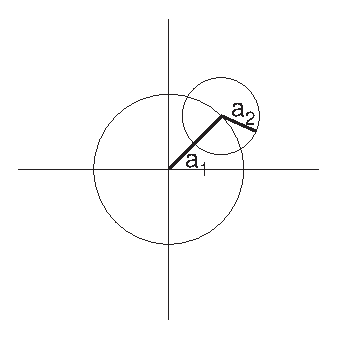
\includegraphics[width=0.5\textwidth]{ch-physical/beating}}
\caption{Phasor representation of beating.\label{fg:beating}} 
\end{figure} 

\begin{figure} 
\centerline{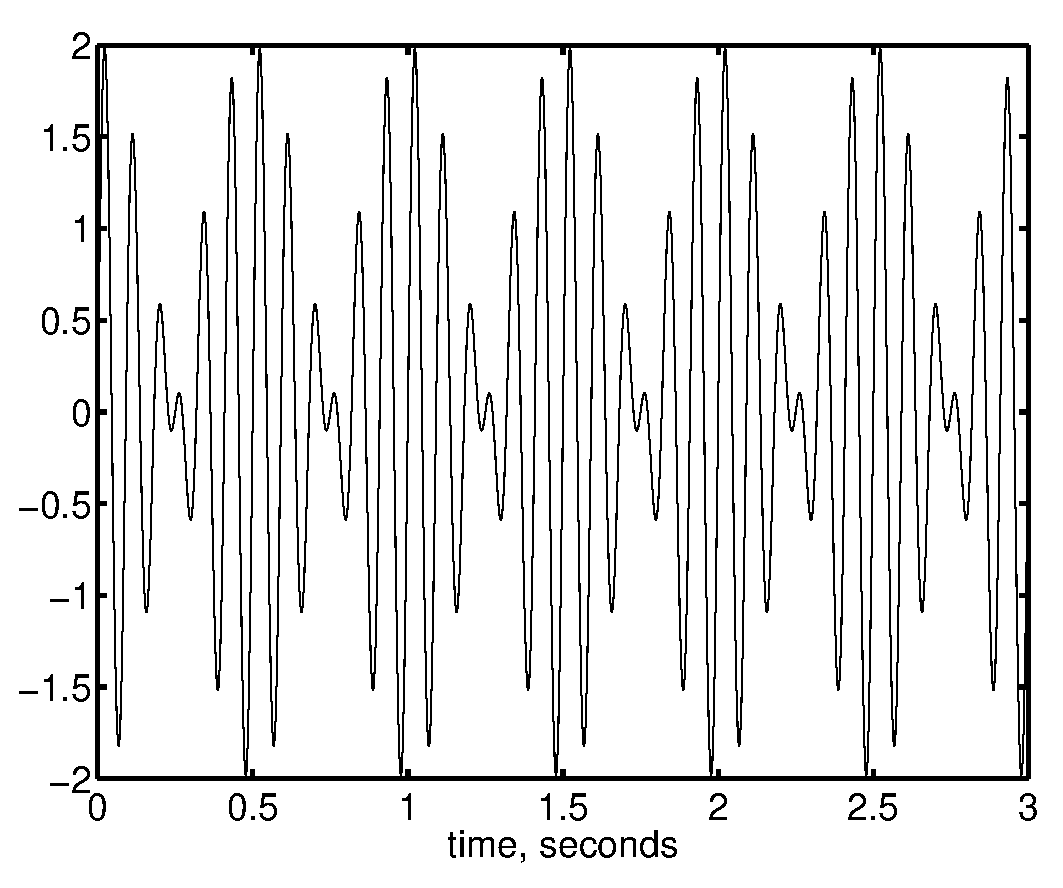
\includegraphics[width=0.5\textwidth]{ch-physical/beating-waveform}}
\caption{Amplitude vs. time representation of beating.\label{fg:beating-waveform}} 
\end{figure} 

This has the form of a complex sinusoid of frequency $\omega$ and
amplitude that is a function of time, $a_1 + a_2 e^{j\delta t}$, that
varies with a frequency of $\delta$. Figure~\ref{fg:beating} presents
the graphical version of this, which looks like a top view of the
amusement park ``octopus'' ride. There are times when the $e^{j\delta
  t}$ adds a factor of up to $a_2$ to the first sinusoid and times
when it subtracts a factor of up to $a_2$. The result is the beating
waveform seen in figure~\ref{fg:beating-waveform} (in this case, the
result of adding 10Hz and a 12Hz sinusoids, which can be seen to
produce a 2Hz ``beat frequency'').

\problemset{
\subsubsection*{MATLAB and Sound Files}
\begin{sloppypar}
\begin{itemize}
\item A MATLAB .m file for demonstrating beating is available at
\url{http://faculty.washington.edu/stiber/pubs/Signal-Computing/beating.m}.
\index{MATLAB code!beating}
\item Audio files to demonstrate beating: a 1000Hz
sine wave at
\url{http://faculty.washington.edu/stiber/pubs/Signal-Computing/1000Hz.au}, a 1005Hz
sine
wave at \url{http://faculty.washington.edu/stiber/pubs/Signal-Computing/1005Hz.au}, and
their
sum, at \url{http://faculty.washington.edu/stiber/pubs/Signal-Computing/beating.au}.
\index{audio files!beating}
\index{sound files|see{audio files}}
\end{itemize}
\end{sloppypar}}

\subsection*{Frequency and Period}

\index{frequency!angular}
\index{$\omega$}
\index{frequency!Hertz (Hz)}
Until now, we've been using $\omega$ as the symbol for the speed of
rotation of a phasor. If $t$ is in seconds (which we will assume is
always the case), then the phasor rotates $\omega/2\pi$ times in one
second, or once in $2\pi/\omega$ seconds. Remembering that our
exponential representation corresponds $\cos \omega t + j \sin \omega
t$, we see that each of these rotations corresponds to $2\pi$ radians
in the oscillation of a sinusoid, and so its units must be
\emph{radians/second}. We will call this \emph{angular frequency}, as
it is the rate of change of the phasor's angle per second. However,
when we speak of periodic physical signals, it is more convenient to
speak of the number of times that the signal repeats per second:
\emph{cycles/second} or \emph{Hertz}. We will use $f$ to refer to
frequencies expressed as Hertz. Since one cycle is $2\pi$ radians, we
can convert between these two units as $\omega = 2\pi f$. In this
book, we will use whichever units are most convenient for each topic;
you'll need to note which is in use.

\index{period!of a sinusoid}
If $\omega$ and $f$ are the number of radians or cycles of a sinusoid
per second, then their reciprocals are the number of seconds per
radian or cycle of rotation. Seconds per radian is only infrequently
used, so we only define a symbol for seconds per cycle, $T = 1/f =
2\pi/\omega$. This is the \emph{period} of a signal in seconds.

\section{Spectra}

Let's return to our discussion of \emph{harmonics}, but now using complex exponentials. We stated earlier that any periodic function could be represented by a sum of weighted harmonics. Let's start with a sum of two sinusoids.
\index{harmonics}
Let's call the first sinusoid's frequency $\omega_0$ and the second's
$\omega_1 = m\omega_0$, $m=2, 3, \ldots$. Their sum is $a_0
e^{j\omega_0 t} + a_1 e^{jm\omega_0 t}$, and there's nothing we can do
to simplify this equation. This ``failure to simplify'' is not a
result of our lack of mathematical sophistication --- there truly is
no simpler representation. Another way of saying this is that
sinusoids at different frequencies are independent or
\emph{orthogonal} to each other. %
\index{sinusoids!orthogonal}%
\index{sinusoids!independent}%
\index{orthogonality}%
\index{independence}%
In general, if we add a large number
of harmonics together, their sum is:
\begin{equation}
\sum_{k=0}^N a_k e^{jk\omega_0 t}
\label{eq:sum-harmonics}
\end{equation}

You'll note that the $k=0$ term of this summation has the value $a_0$
for all time; this is often called the \emph{DC component} of the
\index{DC component}
signal. All other components have frequencies that are integer
multiples (harmonics) of $\omega_0$, the \emph{fundamental
frequency}. Note that a sinusoid with frequency $k\omega_0$ has a
\index{frequency!fundamental}
period of $2\pi/(k\omega_0) = T_0/k$ --- it repeats $k$ times in $T_0$
seconds. This means it \emph{also repeats} every $T_0$ seconds, and since
each term in the summation repeats every $T_0$ seconds, the whole
summation repeats that often, and therefore the period of the signal
represented by the summation is $T_0$. As we said before, such
a summation can in fact be used to represent \emph{any} periodic
function of time. The series of weights, $a_k$, is known as the \emph{Fourier Series}. This \emph{Fourier series} is one of the most
\index{Fourier series|emph}
important and fundamental principles of signal processing. It allows us to look at the \emph{spectrum} of a signal.

\index{spectrum}
You should be familiar already with the term ``spectrum'' as used to
describe the continuous band of colors that white light (sunlight) can
be broken into --- a rainbow. From physics, you know that each color
corresponds to a specific frequency of the visible spectrum. Hence,
the decomposition of white light into colors is actually a form of
frequency analysis. \emph{Frequency analysis} involves the
\index{frequency analysis}
decomposition of a signal into its frequency (sinusoidal) components;
this is also called \emph{spectral analysis}. The multimedia signal
\index{spectral analysis}
waveforms we are concerned with here are basically functions of
time.

At this point, you should recognize that the Fourier series represents
the spectrum of a periodic signal.  It (and other tools) decomposes
signals into spectra defined in terms of sinusoidal (or complex
exponential) components. With such a decomposition, a signal is said
to be represented in the
\emph{frequency domain}; otherwise, usually it is in the \emph{time
domain}. For periodic signals, such a decomposition is the Fourier
Series. For infinite signals (with finite energy), the decomposition
is called a \emph{Fourier Transform}. For finite, discrete signals,
the decomposition is the \emph{Discrete Fourier Transform}.
Recombining the sinusoidal components to reconstruct the original
signal is basically a Fourier synthesis problem or
\emph{inverse Fourier analysis}. 

The weights, $a_k$, of the Fourier Series are usually complex valued. To explain the derivation of the Fourier Series, we therefore need to look at \emph{vectors} in the complex plane.

%%%
%\index{z-transform!properties of}
%\begin{table}
%\caption{Some properties of the z-transform.\label{tb:zt-property}}
%\begin{center}
%\begin{tabular}{|l|c|c|} \hline
%Property      & Time Domain, $Z^{-1}\{\cdot\}$ & z-Domain, $Z\{\cdot\}$ \\ \hline\hline
%Linearity     & $a_1x[n]+a_2y[n]$ & $a_1X(z)+a_2Y(z)$\\ 
%Time shift    & $x[n-k]$       & $z^{-k}X(z)$\\ 
%Scaling in the z-domain 
%              & $a^nx[n]$        & $X(a^{-1}z)$ \\ 
%Time reversal & $x[-n]$        & $X(z^{-1})$\\ 
%Differentiation in the z-domain 
%              & $nx[n]$          & $-z \deriv{X(z)}{z}$ \\ 
%Convolution   & $x[n] \ast y[n]$       & $X(z)Y(z)$ \\ \hline
%\end{tabular}
%\end{center}
%\end{table}
%%%
\subsection{Interlude: Vectors}

\index{vectors|(}
Here is a list of vector operations, most of which you are likely already familiar with. Let $\mathbf{v}$ and $\mathbf{w}$ be arbitrary vectors and
$\vec{\mathbf{x}}, \vec{\mathbf{y}}$ and $\vec{\mathbf{z}}$ be an
orthogonal \emph{basis} (the component vectors that define the
\index{vectors!basis}
coordinate system, which for 3D Cartesian coordinates would be unit
vectors parallel to the $X$, $Y$, and $Z$ axes).  We can then define
the following:

\begin{enumerate}
\item Projection of a vector onto the basis vectors (you may
know these as the \emph{components} of the vector)
\index{vectors!projection}
\index{vectors!components}
\begin{align}
v_x &= \langle\mathbf{v},\vec{\mathbf{x}}\rangle \notag\\
v_y &= \langle\mathbf{v},\vec{\mathbf{y}}\rangle \label{eq:basis-proj}\\
v_z &= \langle\mathbf{v},\vec{\mathbf{z}}\rangle \notag\\ 
\end{align}
and 
\begin{align}
w_x &= \langle\mathbf{w},\vec{\mathbf{x}}\rangle \notag\\
w_y &= \langle\mathbf{w},\vec{\mathbf{y}}\rangle \\
w_z &= \langle\mathbf{w},\vec{\mathbf{z}}\rangle \notag\\ 
\end{align}
\item Expressing a vector using the basis (i.e., as the sum of its
components)
\index{vectors!as sum of components}
\begin{align}
\mathbf{v} &= v_x\vec{\mathbf{x}} + v_y\vec{\mathbf{y}} +
v_z\vec{\mathbf{z}} \label{eq:vec-comps}\\ 
\mathbf{w} &= w_x\vec{\mathbf{x}} + w_y\vec{\mathbf{y}} +
w_z\vec{\mathbf{z}}
\end{align}
\item Inner product of two vectors
\index{vectors!inner product}
\begin{align}
\langle\mathbf{v}, \mathbf{w}\rangle &= v_xw_x +  v_yw_y + v_zw_z
 \label{eq:inner-product}\\
\langle\mathbf{v}, \mathbf{v}\rangle &= v_x^2 +  v_y^2 + v_z^2
\end{align}
You may be familiar with the inner product of a vector with itself as
being its length squared, $|\mathbf{v}|^2$.  When the vector is
complex the inner product is defined as:
\begin{align}
\langle\mathbf{v}, \mathbf{w^*}\rangle &= v_xw_x^* +  v_yw_y^* + v_zw_z^*
 \label{eq:complex-ip}\\
\langle\mathbf{v}, \mathbf{v^*}\rangle &= |v_x|^2 + |v_y|^2 + |v_z|^2
\end{align}
where $^*$ denotes complex conjugate. 

We can also consider arbitrary functions to be more generalized forms
of vectors. If $f(t)$ and $g(t)$ are periodic functions of a
continuous time variable $t$ with period $T$, their inner product is
defined as
\begin{equation}
\langle f, g\rangle = \frac{1}{T}\int_0^T f(t)g^*(t) dt \label{eq:func-ip}
\end{equation}
which is normalized to one by $T$. Intuitively, you can think of this as a ``projection'' of one function onto another, or ``how much'' of of $f$ is in the same ``direction'' as $g$.

\item Vector sum
\index{vectors!sum}
\begin{equation}
\mathbf{v} + \mathbf{w} = 
    (v_x+w_x)\vec{\mathbf{x}}
  + (v_y+w_y)\vec{\mathbf{y}}
  + (v_z+w_z)\vec{\mathbf{z}}
 \label{eq:vec-sum}
\end{equation}
\item Distributive and commutative properties of inner products
\index{vectors!inner product!distributive property}
\index{vectors!inner product!commutative property}
\begin{align}
\langle\mathbf{v} +\mathbf{u} , \mathbf{w}\rangle &=
   \langle\mathbf{v},\mathbf{w}\rangle + \langle\mathbf{u}, \mathbf{w}\rangle
 \label{eq:ip-dist}\\
\langle\mathbf{u}, \mathbf{v}\rangle &= \langle\mathbf{v}, \mathbf{u}\rangle
 \label{eq:ip-commut}
\end{align}
\item $\mathbf{v}$ is \emph{orthogonal} to $\mathbf{w}$
\index{vectors!orthogonal}
\begin{equation}
\langle\mathbf{v}, \mathbf{w}\rangle = 0 \label{eq:orthogonal}
\end{equation}
\item Unit vector
\index{vectors!unit}
\index{unit vector}
\begin{equation}
\langle\mathbf{v}, \mathbf{v}\rangle = v_x^2 +  v_y^2 + v_z^2 =1
 \label{eq:unit-vector}
\end{equation}
\end{enumerate}
\index{vectors|)}

\subsection{Derivation of the Fourier Series}

Here we present frequency analysis tools for continuous time periodic
signals. A periodic signal is defined as: 
\begin{equation}
f(t) = f(t+T)
\end{equation}
where $t$ is a continuous time variable and $T$ is the signal's
period.

The basic mathematical representation of periodic signals is the
Fourier Series, which as we have seen is a weighted sum of
\emph{harmonically related} sinusoids (sinusoids whose frequencies are
all multiples of a single,
\emph{fundamental} one) or complex exponentials. This was first
developed in the nineteenth century by the French mathematician Jean
Baptiste Joseph Fourier to describe heat conduction. Now it has
extensive applications in a variety of problems encompassing many
different fields.

\index{Fourier Series|emph}
The \emph{Fourier Series} description of a periodic function $f(t)$, 
with period $T=2\pi/\omega_0$, is defined
as a weighted sum of complex exponentials:
\begin{equation}
f(t) = \sum_{k=-\infty}^{\infty} c_k e^{jk\omega_0 t}
\label{eq:fs}
\end{equation}
We may think of the exponential signals (or phasors)
\begin{equation}
e^{jk\omega_0 t}, \quad k = \ldots, -2, -1, 0, 1, 2, \ldots
\end{equation}
as a set of basis vectors, where $\omega_0 = 2\pi /T$ is the frequency of
the phasor in radians/second. By our earlier definition, $\omega_0$ is the
\emph{fundmental frequency}. In a Fourier series, the periodic
\index{frequency!fundamental}
function $f(t)$ is expressed in terms of the basis and $c_k$ is the
projection of $f(t)$ onto the basis $e^{jk\omega_0 t}$, just like the
projection $v_x$ of a vector $\mathbf{v}$ onto the basis $\vec{\mathbf{x}}$. The weight, $c_k$, tells us exactly ``how much'' of the signal, $f(t)$, is a result of the frequency $k\omega_0$. From
equation~\ref{eq:func-ip}, the inner product of $f(t)$ and
$e^{jk\omega_0 t}$ is
\begin{equation}
c_k = \langle f(t), e^{jk\omega_0 t}\rangle 
    = \frac{1}{T}\int_0^T f(t)e^{-jk\omega_0 t}dt.
\label{eq:fs-ck}
\end{equation}
where the \emph{Fourier coefficients} $c_k$ are called the
\index{Fourier coefficients|emph} \emph{frequency content} or
\emph{spectrum} of $f(t)$, $k=0, \pm 1, \pm 2, \ldots,
\pm\infty$. This spectrum is just like the familiar shorthand of
writing a vector as a column or row of numbers, with the understanding
that each is the coefficient of one of the basis vectors (i.e., when
we write $\mathbf{v} = [1 2 3]$, what we actually mean is $\mathbf{v}
= 1 \vec{\mathbf{x}} + 2 \vec{\mathbf{y}} + 3 \vec{\mathbf{z}}$).
This is the signal's representation in the \emph{frequency domain},
where frequency is the coordinate (in other words, the signal
expressed as a function of frequency).  Similarly, $f(t)$ is the
signal's \emph{time domain} representation, where time is the
coordinate. Notice that the Fourier series transforms a finite
(periodic), continuous signal in the time domain into an infinite
(because the values of $k$ range from $-\infty$ to $+\infty$),
discrete (because $k$ only takes on integer values) spectrum in the
frequency domain.

\subsubsection{Alternative Derivation of the Fourier Series [\textsc{Optional}]}

Another way to derive the formula for the $c_k$ is as follows.  The aim of this derivation is to plug in the Fourier Series definition of $f(t)$ into the equation for $c_k$ and see if we can get exactly $c_k$ back by manipulating the equation. We
first multiply both sides of (\ref{eq:fs}) by the phasor
$e^{-jl\omega_0 t}$ ($l=\ldots, -2,-1,0,1,2,\ldots$) and then
integrate both sides of the resulting equation over a single period
[0, T],
\begin{align}
c_k=\frac{1}{T}\int_0^T f(t)e^{-jl\omega_0t}dt
&= \frac{1}{T}\int_0^T \sum_{k=-\infty}^{\infty} c_k e^{jk\omega_0t}
e^{-jl\omega_0 t}dt \notag\\
&= \sum_{k=-\infty}^{\infty} c_k \frac{1}{T}\int_0^T
e^{j(k-l)\omega_0t}dt
\label{eq:fs-ck2}
\end{align}
Note that
\begin{align}
\frac{1}{T}\int_0^T e^{j(k-l)\omega_0t}dt
&= \frac{1}{T}\left.\frac{e^{j(k-l)\omega_0t}}{j(k-l)\omega_0}
               \right|_0^T \notag\\
&= \frac{e^{j(k-l)\omega_0T} - 1}{j(k-l)\omega_0T}
    \label{eq:fs1}
\end{align}

Equation~(\ref{eq:fs1}) has two different solutions, depending on
whether $k=l$ or not. Let's make the substitution $u=k-l$. So, when
$k=l$, $u=0$, and the numerator and denominator of~(\ref{eq:fs1}) are
both zero. We therefore use L'H\^{o}pital's rule to find the limit:
\index{l'H\^{o}pital's rule}
\begin{align}
\lim_{u \rightarrow 0}
   \frac{e^{ju\omega_0T} - 1}{ju\omega_0T}
  & = \left.\frac{\deriv{}{u}\left(e^{ju\omega_0T} - 1\right)}
                   {\deriv{}{u}ju\omega_0T}\right|_{u=0} \notag\\
  & = \left.\frac{j\omega_0Te^{ju\omega_0T}}{j\omega_0T}\right|_{u=0}
        \notag\\
  & = \frac{j\omega_0T}{j\omega_0T} \notag\\
  & = 1
\end{align}

For the case of $k \neq l$, let's rewrite the numerator
of~(\ref{eq:fs1}) as $\cos(k-l)\omega_0T + j\sin(k-l)\omega_0T -
1$. Remember that $\omega_0=2\pi/T$, and so $\omega_0T=2\pi$. Since
both $k$ and $l$ are integers and $k \neq l$, their difference is an
integer; let's call that integer $m$. The numerator then becomes
$\cos2\pi m + j\sin2\pi m - 1$. We know that $\cos2\pi m = 1$ and
$\sin2\pi m = 0$, and so the numerator is zero. On the other hand, the
denominator of~(\ref{eq:fs1}) is $j2\pi m \neq 0$, and
so~(\ref{eq:fs1}) is zero.

In summary,
\begin{equation}
\frac{1}{T}\int_0^T e^{j(k-l)\omega_0t}dt
= \left\{\begin{array}{ll}
                        1 & k=l \\
                        0 & k \neq l
          \end{array}\right.
 \label{eq:orth-sines}
\end{equation}
From the review at the beginning of this chapter (more specifically,
the definition of the inner product of two periodic function
in~(\ref{eq:func-ip})), this yields the interesting revelation that
complex sinusoids at different frequencies are orthogonal (and so, by
extension, can serve as an orthogonal basis).
\index{complex sinusoids!as an orthogonal basis}

Using~(\ref{eq:orth-sines}), equation~(\ref{eq:fs-ck2}) becomes
\begin{equation}
\frac{1}{T}\int_0^T f(t)e^{-jl\omega_0t}dt = c_l, 
\quad l=\ldots, -2, -1, 0, 1, 2, \ldots
\end{equation}
We got the same result as~(\ref{eq:fs-ck}).

\subsubsection{Real-Valued Signals}

In general, the Fourier coefficients $c_k$ are complex valued. If the
periodic signal $f(t)$ is real valued (the kind of signals we're
concerned with here), the $c_k$ satisfy the condition,
\begin{equation}
c_k = c_{-k}^*
\label{eq:fs-cs3}
\end{equation}
Consequently, 
\begin{equation}
|c_k|^2 =|c_{-k}^*|^2
\label{eq:real-f-pspec}
\end{equation}

Since $c_k$ is the (amplitude) spectrum of $f(t)$, $|c_k|^2$ is the
\emph{power spectrum}. Equation~(\ref{eq:real-f-pspec}) tell us that
the power \index{power spectrum} spectrum is a symmetric (or ``even'')
function of frequency. Also, when $f(t)$ is real, we can further
decompose the Fourier Series. Equation ~(\ref{eq:fs}) becomes
\begin{align}
f(t) &= \sum_{k=-\infty}^{\infty} c_k e^{j k\omega_0 t} \notag\\
&= c_0+\sum_{k=1}^{\infty} c_k e^{j k\omega_0 t}
+\sum_{k=-1}^{-\infty} c_k e^{jk\omega_0 t} 
&&\text{(split sum into 0/+/- parts)}
\notag\\
&= c_0+\sum_{k=1}^{\infty} c_k e^{jk\omega_0t}+
\sum_{k=1}^{\infty} c_{-k} e^{-jk\omega_0 t} 
&&\text{(distribute -1 into second sum)}
\notag\\
&= c_0+\sum_{k=1}^{\infty} [c_k e^{jk\omega_0t}+
c_{-k} e^{-jk\omega_0 t}] 
&&\text{(combine common sum)}
\notag\\
&= c_0+\sum_{k=1}^{\infty} [c_k e^{jk\omega_0t}+
(c_{-k}^* e^{jk\omega_0 t})^*] 
&&\text{(double conjugate)}
\notag\\
&= c_0+\sum_{k=1}^{\infty} [c_k e^{jk\omega_0t}+
(c_k e^{jk\omega_0 t})^*] 
&&\text{(real signal: $c_k = c_{-k}^*$)}
\notag\\
&= c_0+2\sum_{k=1}^{\infty} \Real[c_k e^{jk\omega_0t}]
&&\text{($a + a^* = 2\Real(a)$)}
\label{eq:fs-freal1}
\end{align}

With your help in the next self-test exercise, we get
\begin{equation}
f(t)=c_0+2\sum_{k=1}^{\infty} \Real(c_k)\cos k\omega_0t
-2\sum_{k=1}^{\infty} \Imag(c_k)\sin k\omega_0t
\label{eq:fs-freal2}
\end{equation}
where 
\begin{align}
\Real(c_k) &= \frac{1}{T}\int_0^T f(t)\cos(k\omega_0t)dt \label{eq:cosproject}\\
\Imag(c_k) &= -\frac{1}{T}\int_0^T f(t)\sin(k\omega_0t)dt \label{eq:sinproject}
\end{align}
from~(\ref{eq:fs-ck}) and Euler's formula. You can view equations \ref{eq:cosproject} and \ref{eq:sinproject} as the projection of $f(t)$ onto cosine and sine functions in the same way that the previous definition of $c_k$ was the projection of $f(t)$ onto complex exponentials. This representation of $c_k$ does not require any complex number arithmetic, but it is often more cumbersome to carry out the integration using cosines and sines, rather than phasors.

Examples of periodic signals that are frequently encountered in
practice are square waves, rectangular waves (both being used as
timing signals in electronics), triangle waves, and of course
sinusoids and complex exponentials. In the next example, we will use
the Fourier series to analyze some of these.

\problemset{
\subsubsection{Self-Test Exercises}

See~\ref{sc:ch1ex} \#\ref{it:ch1ex8}--\ref{it:ch1ex9} for answers.

\begin{enumerate}
\item Prove the relationship in~(\ref{eq:fs-cs3}).
\item From equation~(\ref{eq:fs-freal1}), derive~(\ref{eq:fs-freal2}). \emph{Hint}: Use the fact that equation~(\ref{eq:fs-freal1}) is a real signal to simplify the complex multiplication.
\end{enumerate}}

\subsubsection*{Example: Fourier series of a general square wave}

\index{Fourier Series!of a square wave} The simplest type of square
wave has a 50\% duty cycle: that is, 50\% of the time
$f(t)$ takes on the value of 1 and 50\% of the time it has the value
-1. Let's do a bit more general of a case. We will consider a train of
rectangular pulses (a kind of square wave, but shifted upward and
scaled so that it has a minimum of zero and a maximum of $V_0$) with
pulse duration $\tau$ and period $T$ seconds. This waveform can be
expressed as
\begin{equation}
f(t) = \left\{\begin{array}{ll}
        0   & \text{region a } (nT\leq t < nT+t_0) \\
        V_0 & \text{region b } (nT+t_0 \leq t < nT+t_0+\tau)\\
	0   & \text{region c } (nT+t_0+\tau \leq t < (n+1)T)
        \end{array}\right.
\quad n = 0 , 1, 2, \ldots
\end{equation}
The waveform is plotted in figure~\ref{fig:fs-pulse} with example regions shown. 

\begin{figure}
\centerline{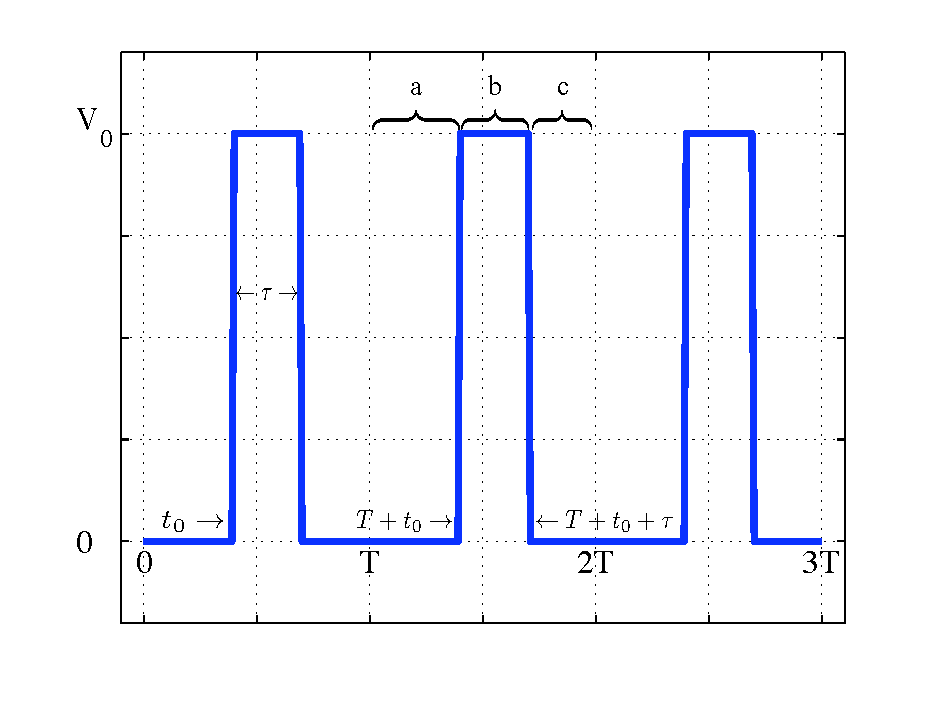
\includegraphics[width=5in]{ch-physical/fs_pulse}}
\caption[A train of periodic rectangular pulses]{A train of periodic
rectangular pulses with period $T$, pulse width $\tau$, and
initial pulse start at $t_0$.
\label{fig:fs-pulse}}
\end{figure}

There are a few general observations we can make of this signal: the
first, that the pulse duration $\tau$ is a variable, so it can be wide
or narrow, thus changing the duty cycle. When it is really narrow, the
signal becomes a train of impulses; when it is on the order of
$\tau=T/2$, it is called ``50\% duty cycle''. The second observation
is that $t_0$ changes the pulse's phase.

According to~(\ref{eq:fs-ck}), the Fourier coefficients $c_k$ are
\begin{align}
c_k &= \frac{1}{T}\int_0^{t_0} 0e^{-jk\omega_0 t} dt
      +\frac{1}{T}\int_{t_0}^{t_0+\tau}V_0e^{-jk\omega_0 t}dt 
      +\frac{1}{T}\int_{t_0+\tau}^{T}0e^{-jk\omega_0 t}dt 
      \label{eq:sq-fs1}\\
    &=\frac{1}{T}\int_{t_0}^{t_0+\tau}V_0e^{-jk\omega_0 t}dt 
      \label{eq:sq-fs2}\\
    &=\frac{V_0}{T}\left[\frac{e^{-jk\omega_0t}}
                               {-jk\omega_0}\right]_{t_0}^{t_0+\tau}
       \label{eq:sq-fs3}\\
    &=\frac{V_0}{-jk\omega_0T}[e^{-jk\omega_0(t_0+\tau)}
                               -e^{-jk\omega_0(t_0)}]
\label{eq:fs-pul-cn1}
\end{align}
In equation~(\ref{eq:sq-fs1}), the integral defining the Fourier
coefficients in~(\ref{eq:fs-ck}) has been broken into three parts for
the three ``segments'' of the square wave: $f(t)=0$ (region a, when $nT\leq t <
nT+t_0$), $f(t)=V_0$ (region b, when $nT+t_0 \leq t < nT+t_0+\tau$), and
$f(t)=0$ (region c, when $nT+t_0+\tau \leq t < (n+1)T$). The first and third
terms are equal to zero, leaving only the middle term, which is just
the integral of an exponential. If we remember that the derivative of
an exponential $\deriv{e^{at}}{t}$ is $ae^{at}$, then the
anti-derivative from~(\ref{eq:sq-fs2}) to~(\ref{eq:sq-fs3}) should
make sense. Finally, we just need to evaluate the expression
in~(\ref{eq:sq-fs3}) between the two limits $t_0$ and $t_0+\tau$ to
yield~(\ref{eq:fs-pul-cn1}).

The middle steps are left for your homework; let's skip to the result:
\begin{equation}
c_k=
  \underbrace{\frac{V_0\tau}{T}
     \frac{\sin(k\omega_0\tau/2)}{k\omega_0\tau/2}}_{\mathrm{magnitude}}
  \underbrace{e^{-jk\omega_0(t_0+\tau/2)}}_{\mathrm{phase}}
\label{eq:fs-pul-cn2}
\end{equation}
This is just the polar representation of a complex valued $c_k = R
e^{j\theta}$.  The phase $\theta$ or angle of $c_k$ is
\begin{equation}
\theta=-k\omega_0 \left(t_0+\frac{\tau}{2}\right)
\end{equation}
Let's define $\alpha=k\omega_0 \tau/2$, and take a look at the
magnitude in~(\ref{eq:fs-pul-cn2}). This function occurs frequently
enough in modern communication theory to be given a name: the sampling
function, or \emph{sinc}. We define
\index{sinc function}

\begin{equation}
\sinc\alpha = \frac{\sin\alpha}{\alpha}
\end{equation}

We note that $\sinc\alpha$ is zero whenever $\alpha$ is an integral
multiple of $\pi$; that is,
\begin{equation}
\sinc n\pi = 0, \quad n=1, 2, 3, \ldots
\label{eq:fs-Snpi}
\end{equation}

When $\alpha$ is zero, the function is indeterminate, but it is easy
to show that its value is unity: 
\begin{equation}
\sinc 0 = 1
\label{eq:fs-S0}
\end{equation}

\begin{figure}
\centerline{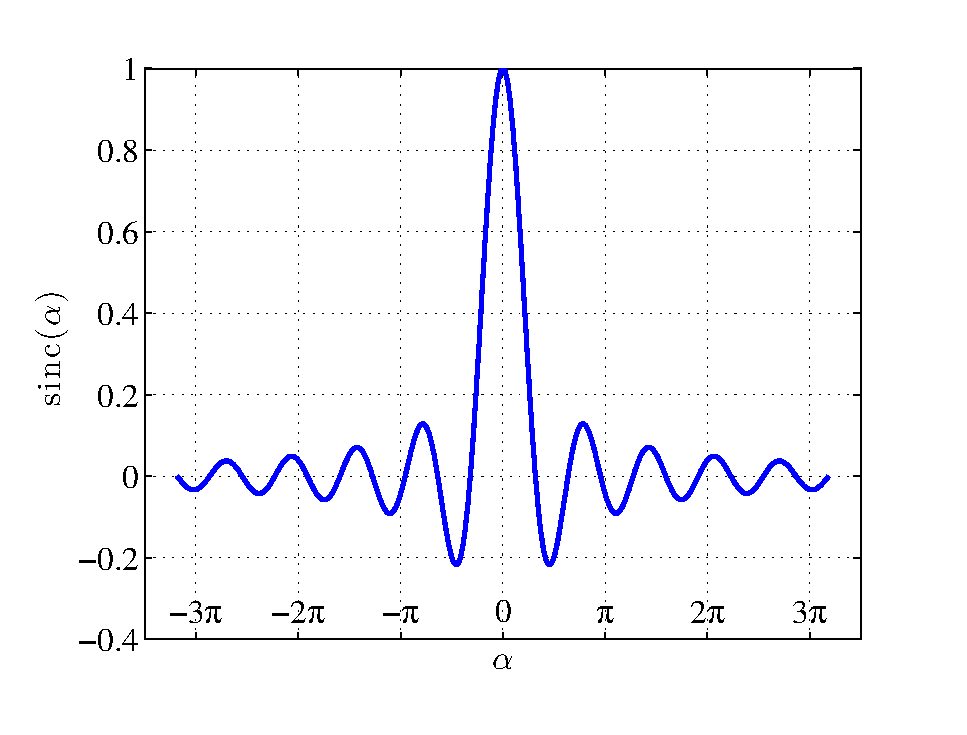
\includegraphics[height=3in]{ch-physical/fs_sinc}}
\caption{The sinc function.\label{fig:sinc}}
\end{figure}

The magnitude of $\sinc\alpha$ therefore decreases from unity at
$\alpha=0$ to zero at $\alpha=\pi$. As $\alpha$ increases from $\pi$
to $2\pi$, $\sinc\alpha$ increases from zero to a maximum less than
unity. As $\alpha$ continues to increase, the successive maxima become
smaller because the numerator of $\sinc\alpha$ can not exceed unity
while the denominator increases. Also, $\sinc\alpha$ shows even
symmetry. Figure~\ref{fig:sinc} shows the sinc function.

From~(\ref{eq:fs-S0}), we know that $c_0$ is 
\begin{equation}
c_0=\frac{V_0\tau}{T}
\end{equation}

Substituting $c_0$ and $c_k, k=1, 2,3,\ldots$
into~(\ref{eq:fs-freal1}), the Fourier series of $f(t)$ is
\begin{align}
f(t)&= \frac{V_0\tau}{T} +2\Real\left\{\sum_{k=1}^{\infty}
          \frac{V_0\tau}{T}
          \frac{\sin(k\omega_0\tau/2)}{k\omega_0\tau/2}
          e^{-jk\omega_0(t_0+\tau/2)}e^{jk\omega_0t}\right\} 
       \label{eq:fs-pulsef1}\\ 
    &= \frac{V_0\tau}{T}
       + 2\Real\left\{\sum_{k=1}^{\infty}\frac{V_0\tau}{T}
            \frac{\sin(k\omega_0\tau/2)}{k\omega_0\tau/2}
            e^{jk\omega_0(t-t_0-\tau/2)}\right\} && \text{(collect exponents)}
       \label{eq:fs-pulsef2}\\
    &= \underbrace{\frac{V_0\tau}{T}}_{c_0}
       + \underbrace{\frac{2V_0\tau}{T} \sum_{k=1}^{\infty}
           \sinc(k\omega_0\tau/2)}_{c_k}
           \underbrace{\cos[k\omega_0(t-t_0-\tau/2)]}_{\text{harmonically
               related sinusoids}} && \text{(apply Euler's)}
\label{eq:fs-pulsef}
\end{align}
In~(\ref{eq:fs-pulsef1}), we have used the knowledge of this being a
real-valued signal. We collected the exponents to
get~(\ref{eq:fs-pulsef2}), then factored out the $V_0\tau/T$, applied
Euler's formula to the exponential, and finally retained only the real
part of each term of the summation to yield~(\ref{eq:fs-pulsef}).

\begin{figure}
\centerline{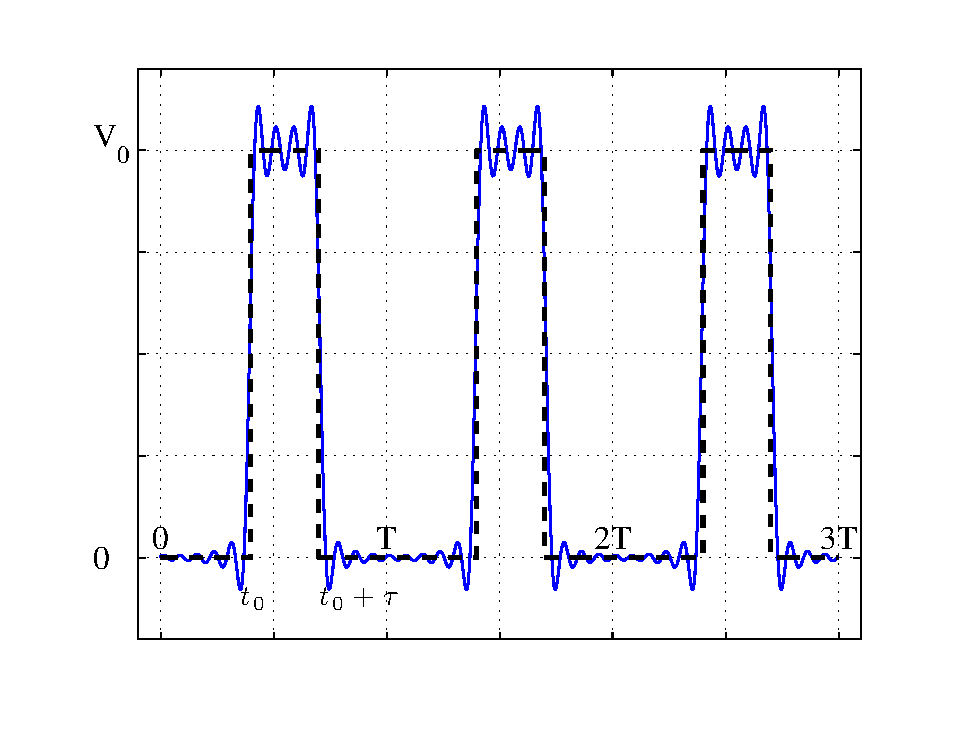
\includegraphics[width=5in]{ch-physical/fs_pulsef12}}
\caption[First 12 terms in the Fourier series for a periodic sequence
of rectangular pulses]{The Fourier series for a periodic sequence of
rectangular pulses. The first 12 harmonic terms in
summation~(\protect\ref{eq:fs-pulsef}) are included. The ideal pulse
train is shown as dashed lines. The period is $T=1$, the initial point
$t_0=0.5$ and the pulse width $\tau=0.3333$.
\label{fig:fs-pulsef}}
\end{figure}

\begin{figure}
\centerline{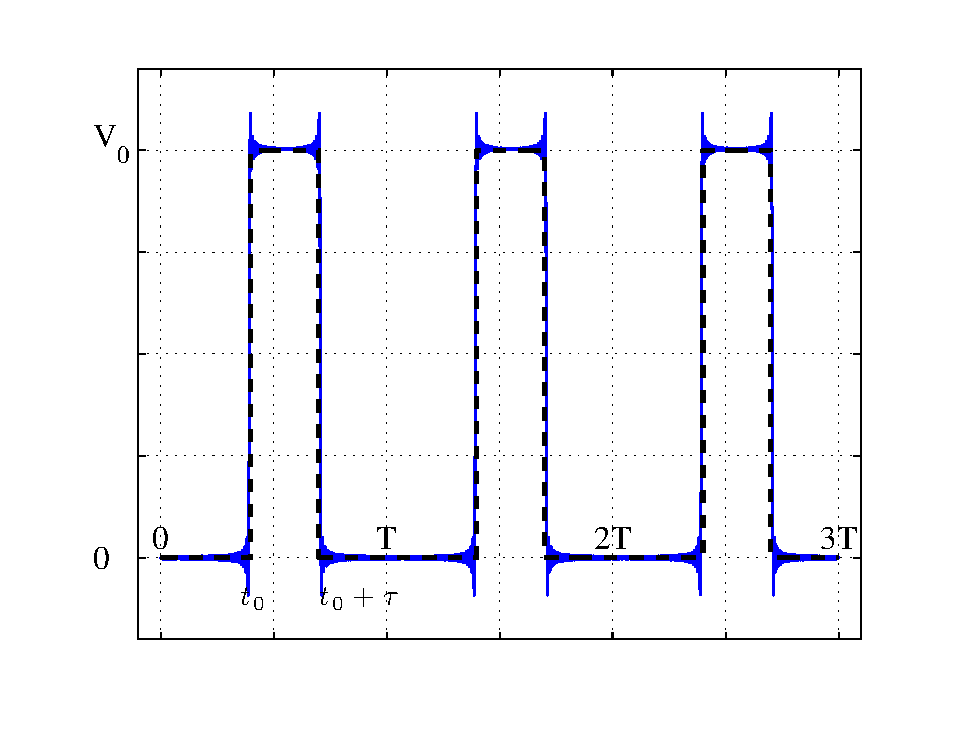
\includegraphics[width=5in]{ch-physical/fs_pulsef100}}
\caption[First 100 terms in the Fourier series for a periodic sequence
of rectangular pulses]{The Fourier series for a periodic sequence of
rectangular pulses. The sum of the first 100 terms is shown, as in
figure~\protect\ref{fig:fs-pulsef}.
\label{fig:fs-pulsef2}}
\end{figure}

Now, a train of pulses is represented by an infinite number of
sinusoidal waves. How well can it be approximated by a finite number?
Look at figure~\ref{fig:fs-pulsef}. The solid curve shows the sum of
the first 12 terms of the signal's Fourier series; it looks like a
pulse train modulated by a sinusoid. The ideal pulses are shown as
dashed lines. The approximation gets better when more terms are used,
as in figure~\ref{fig:fs-pulsef2}.

Let's construct the signal's \emph{spectrum}: a plot of its Fourier
\index{spectrum}
coefficients. We first consider $|c_k|$ expressed in terms of the
fundamental frequency $f_0$, remembering that $\omega_0=2\pi f_0$:
\begin{equation}
|c_k|=\frac{V_0\tau}{T}|\sinc(k\pi f_0 \tau)|
\label{eq:fs-pulseabscn}
\end{equation} 

The magnitude of any $c_k$ is obtained from~(\ref{eq:fs-pulseabscn})
by using the known values of pulse width $\tau$ and signal period
$T=1/f_0$, and selecting the desired value of $k$ $(k=0, 1, 2,
\ldots$). Instead of evaluating~(\ref{eq:fs-pulseabscn}) at these
discrete frequencies, let us sketch the envelope of $|c_k|$ by
considering the frequency $kf_0$ to be a continuous variable. That is,
though $f=kf_0$ can really only take on the discrete values (the
harmonic frequencies - $0, f_0, 2f_0, 3f_0, \ldots$) we may think
of $k$ for the moment as a continuous variable. When $f$ is zero,
$|c_k|$ is $V_0\tau/T$, and when $f$ has increased to
$1/\tau$, $|c_k|$ is zero.  In fact from (\ref{eq:fs-Snpi}) when
$f\pi\tau = m\pi$ ($m=1,2,3,\ldots$), $\sinc(f\pi\tau)=0$, which
yields zeros at frequencies $f = m/\tau$.

\begin{figure}
\centerline{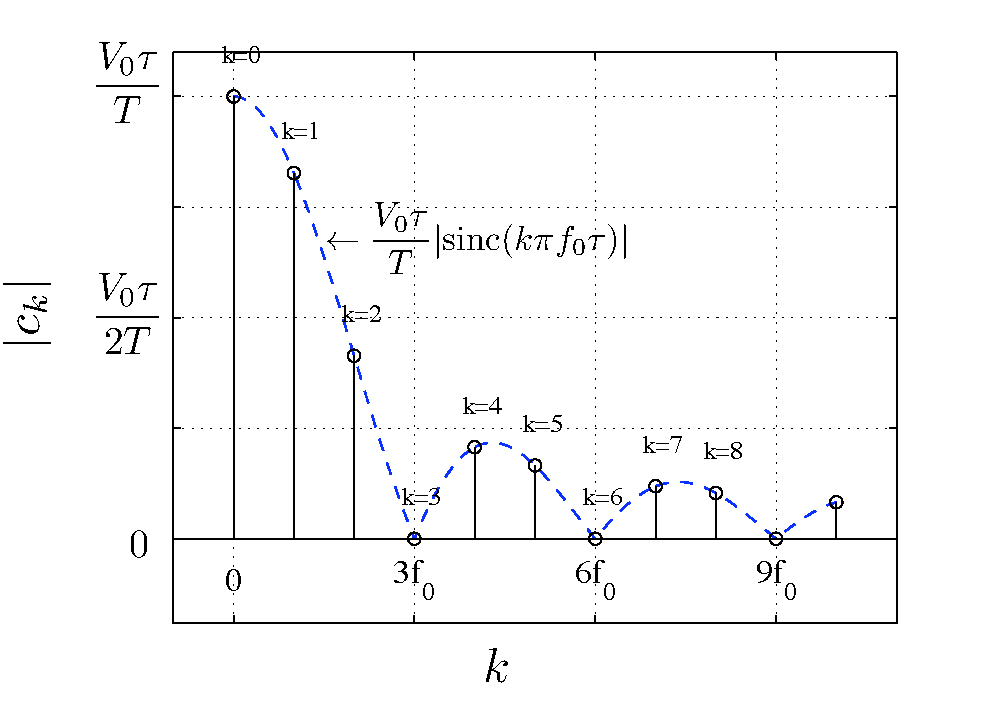
\includegraphics[height=4in]{ch-physical/fs_pulsecn}}
\caption[Spectrum of a periodic sequence of rectangular pulses]{The
spectrum of a periodic sequence of rectangular pulses: the magnitude
of $c_k$ vs. frequency $f=kf_0$, where $f_0=1/T$ (light gray vertical
lines).  The envelope for continuous $k$ is plotted as the black
curve. Zero points in the spectrum $|c_k|$ are at $kf_0=n/T=m/\tau$,
$m=1,2,3,\ldots$.
\label{fig:fs-pulsecn}}
\end{figure}

The resultant line spectrum and envelope are plotted in
figure~\ref{fig:fs-pulsecn}.  The figure is the plot of the envelope
of the Fourier coefficients $\{c_k\}$ (the spectrum of the periodic
sequence of rectangular pulses), versus frequency $f=kf_0$. The
magnitude of its peaks decays at the rate of $1/k$.

\begin{figure}
\centerline{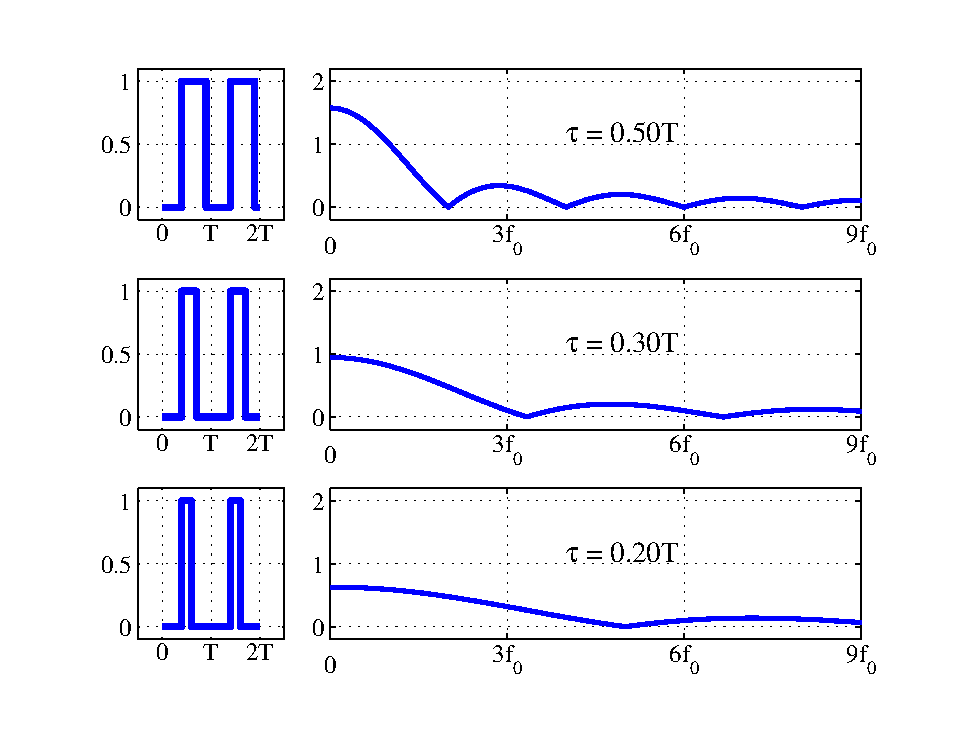
\includegraphics[height=4in]{ch-physical/fs_pulsecntau}}
\caption[Spectrum of a periodic sequence of rectangular 
pulses; varying pulse width]{The spectrum of a periodic sequence of
rectangular pulses, when $T$ is fixed and the pulse width $tau$
varies.
\label{fig:fs-pulsecntau}}
\end{figure}

\begin{figure}
\centerline{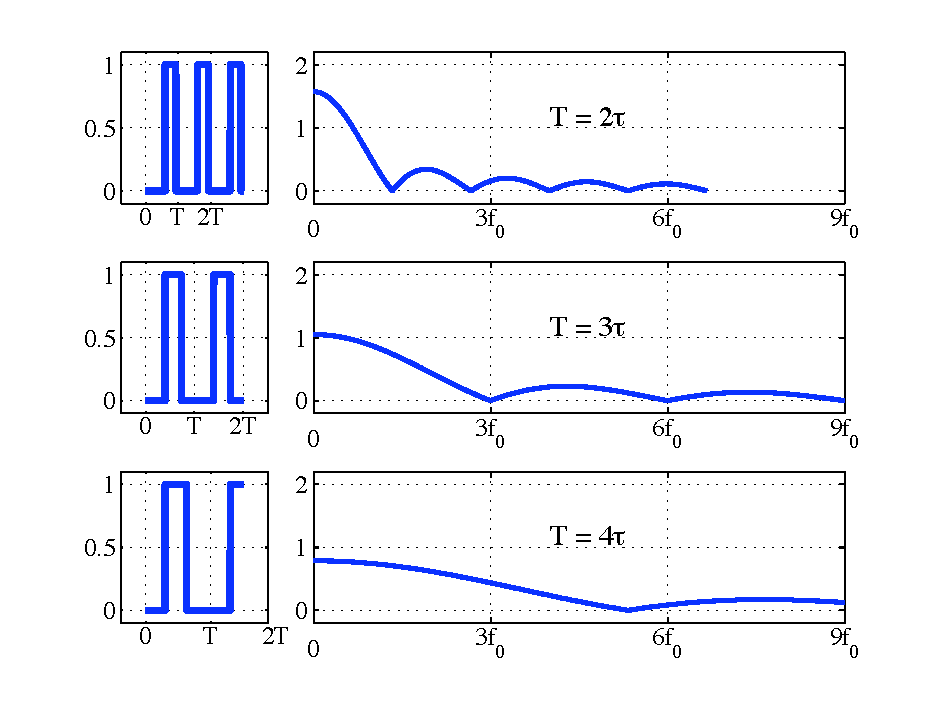
\includegraphics[height=4in]{ch-physical/fs_pulsecnT}}
\caption[Spectrum of a periodic sequence of rectangular  
pulses; varying period]{The spectrum of a periodic sequence of
rectangular pulses with fixed pulse width $tau$ and varying period
$T$.
\label{fig:fs-pulsecnT}}
\end{figure}

There are several observations which we may make that relate
changes in the line spectrum to changes in the graph of rectangular pulses
given in figure~\ref{fig:fs-pulsecn}. Firstly, note that the width of the envelope
depends upon changes in $\tau$, the pulse width. In fact,
the \emph{shape} of the envelope does not vary with changes in $T$;
instead, changes in $T$ correspond to changes in the frequency
interval between spectral lines. If the pulse period $T$ is increased
($f_0$ is decreased), the number of spectral lines between zero
frequency and $1/\tau$ increases and the amplitude of each line
decreases. Figures~\ref{fig:fs-pulsecntau} and~\ref{fig:fs-pulsecnT}
illustrate this.

A shift in the phase $t_0$ does not change the line spectrum,
that is, $|c_k|$ is not a function of $t0$. The \emph{phase} of the
frequency components \emph{do} change with the choice of $t_0$ (we just
haven't plotted those).

When talking about the generalized square wave, with fixed period $T$
and pulse width $\tau$ increasing or decreasing, the result is a
family of different waveforms. When $\tau = T/2$, we have a 50\% duty
cycle square wave. When $\tau$ takes on different percentages of $T$,
we get different duty cycles. Also, when $\tau$ becomes really small,
the waveform become a train of impulses.

\problemset{
\subsubsection{Self-Test Exercise}

See~\ref{sc:ch1ex} \#\ref{it:ch1ex10} for the answer.

\begin{enumerate}
\item Prove (\ref{eq:fs-S0}).
\end{enumerate}}



\section{Problems}

\begin{enumerate}
\item The differential equation for a tuning fork can be written as $\sderiv{x(t)}{t} = -\frac{k}{M} x(t) $ where $M$ is the mass of the tuning fork, $k$ is a constant, and $x(t)$ is the displacement of the tuning fork endpoints. Discuss how the mass of the tuning fork affects the frequency at which it vibrates. Hint: relate the given equation to equation \ref{eq:diffeq1}.
\item What musical instruments might be governed by properties
  analogous to that of a tuning fork? 
\item When you add two sinusoids with frequencies that differ by
  $\delta$, the result is beating. Imagine you're tuning a guitar.  As
  the two strings get closer together in tone, what happens to the
  beat frequency? Show how this result is predicted by the sum of the
  complex sinusoids.
\item A complex number can be written in rectangular coordinates as $z
  = x + j y$. Write the relations to calculate the polar form, $z=(r,
  \theta)$ or $z = r e^{j\theta}$.

\item Using Euler's formula, express $\cos x$ and $\sin x$ as a
  combination of complex exponentials. Recall that Euler's Formula is given by: $e^{\pm j\omega t}=\cos(\omega t) \pm j \sin(\omega t)$.

\item Find expressions for the following as complex exponentials:
	\begin{enumerate}
	\item1 
	\item $j$
	\item $1 + j$, $(1 + j\sqrt{3})/2$
	\end{enumerate}

\item Compute $[(1+j\sqrt{3})/2]^2$ and $(1+j)^4$ directly using: 
  \begin{enumerate}
  \item Rectangular representations.
  \item Complex exponentials.
  \end{enumerate}

\item Show that $(z_xz_y)^* = z_x^* z_y^*$.


\item Express $|z|^2$ as a function of $z$ and $z^*$.


\item Given the following equations:
\begin{align*}
x_1(t) &= 5 \sin(2\pi(200)t +0.5\pi) \\
x_2(t) &= 5 \sin(2\pi(200)t - 0.25\pi) \\
x_3(t) &= 5 \sin(2\pi(200)t +0.4\pi) \\
x_4(t) &= 5 \sin(2\pi(200)t - 0.9\pi) 
\end{align*}

\begin{enumerate}
\item Using pencil and paper: Express   $x_1(t)$ through $x_4(t)$ as complex exponentials. 

\item Create the sum sinusoid, $x_5(t)=x_1(t)+x_2(t)+x_3(t)+x_4(t)$. Express   $x_5(t)$ as a sum of complex exponentials. 	

 \item Using complex exponentials, express the amplitude and phase of $x_5(t)$ (use pencil and paper with the aide of a graphing calculator, spreadsheet, or MATLAB).

 \end{enumerate}
	
\item What is the period of $e^{-j\frac{\pi}{4}t}+e^{-j\frac{\pi}{2}t}$ ?
\item What is the period of $e^{-j \omega_0 t}+e^{-j 5\omega_0 t}$ ?
\item Implement a  \texttt{Complex} class for representing
  complex numbers in an object oriented programming language (C++, C\#, Java, python, etc.).  Your class should include at least the following
  methods:
  \begin{itemize}
  \item \texttt{add()}
  \item \texttt{multiply()}
  \item \texttt{real()}
  \item \texttt{imag()}
  \item \texttt{magnitude()}
  \item \texttt{angle()}
  \end{itemize}

  Document your code so that this class could be used by someone else.
  Write a test program that exercises all of this class' methods. 

\item Derive equation~(\ref{eq:fs-pul-cn2}) from
  equation~(\ref{eq:fs-pul-cn1}).

\item Determine the coefficients of the Fourier series for the following signals:
\begin{enumerate}
\item The sinusoid \[x(t) = \cos \frac{\pi}{3} t\]
\item The sawtooth waveform \[ x(t) = t-\lfloor t \rfloor \]
\item The rectified wave \[ x(t) = |\cos(\frac{\pi}{3} t)| \]
\end{enumerate}
\end{enumerate}

\section{Further Reading}

\begin{itemize}
\item James H McClellan, Ronald W. Schafer, and Mark A. Yoder,
  \textit{DSP First: A Multimedia Approach}, Prentice Hall, 1998,
  chapters 1--3 (\S 3.1--3.4), appendix A.
\item Martin D. Levine, \textit{Vision in Man and Machine},
  McGraw-Hill, 1985, chapter 1, sections 2.1, 2.2.
\item Robert S. Tannenbaum, \textit{Theoretical Foundations of
  Multimedia}, Computer Science Press, 1998, chapters 1 \& 2.
\item Donald Hearn \& M. Pauline Baker, \textit{Computer Graphics},
  Second Edition, Prentice Hall, 1997, sections 2.1--2.4.
\item A. Murat Tekalp, \textit{Digital Video Processing}, Prentice
  Hall, 1995, chapters 1 \& 2. 
\end{itemize}


% -*-LaTeX-*-

% $Log: computer-signals.tex,v $
% Revision 1.8  2010/03/16 00:26:08  stiber
% Minor clarification.
%
% Revision 1.7  2007/12/25 17:46:12  stiber
% Some final cosmetic changes.
%
% Revision 1.6  2007/12/08 17:22:10  stiber
% Minor edits and corrections for Winter 2008.
%
% Revision 1.5  2007/03/20 23:52:12  stiber
% Cleaned up and updated LaTeX.
%
% Revision 1.4  2007/03/10 19:25:06  stiber
% Updated chapter for stand-alone textbook. Incorporated suggestions
% from Donald Christopherson.
%
% Revision 1.3  2006/03/27 23:35:14  stiber
% Fixed mistakes in end-of-chapter problem.
%
% Revision 1.2  2004/03/29 19:51:15  stiber
% Updated for Spring 2004 and new textbook (DSP First).
%
% Revision 1.1  2004/02/19 00:23:17  stiber
% Initial revision
%

\chapter{Signals in the Computer}
\label{ch:computer-signals}

In chapter~\ref{ch:physical-signals}, you were introduced to the
nature of physical signals and how they can be described
mathematically.  In this chapter, we move onward to discuss how these
``real world,'' analog signals end up inside computers: analog to
digital conversion (A/D conversion, or ADC). We then develop the first
little bit of a fundamental mathematical representation of such
\emph{discrete} signals. In the process, we visit the problems that
digitization creates. At the end of this chapter, you should have a
basic grasp of how ADC works and the tradeoffs involved in A/D
parameters versus the characteristics of the analog signal.

\section{From the physical to the digital}

Physical signals fundamentally involve application of energy to cause
some physical quantity to change. For instance, sound is carried by
waves of changing air pressure; images are patterns of emitted and/or
reflected light. On the other hand, computer signals are collections
of binary numbers --- vectors for sound, 2D arrays for images, or
sequences of 2D arrays for video. The process of bridging this gap is
the process of connecting the analog world to the digital
computer, or \emph{data acquisition}. There are three parts to this
\index{data acquisition}
process:
\begin{enumerate}
\item transduction,
\item sampling,
\item and quantization.
\end{enumerate}

\begin{figure}
\centerline{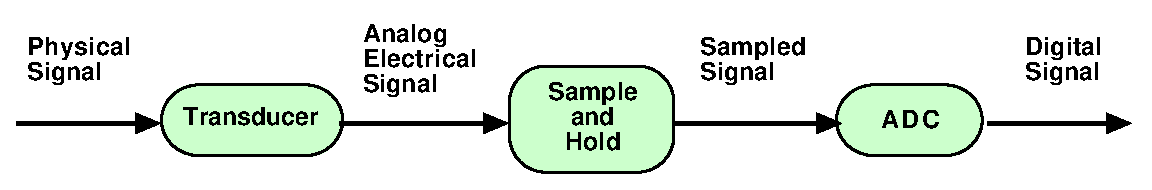
\includegraphics[width=\textwidth]{ch-computer/adc}}
\caption{Block diagram of the data acquisition process.\label{fg:adc}}
\end{figure}

Figure~\ref{fg:adc} shows these three steps and the intervening
representations of the signal.  This is an important point: the
``real'' signal is the physical one; what we seek to do is to produce
a \emph{representation} of this signal within the computer. Our goal
is that this representation will carry all the information of interest
that the original had. In this chapter, I will concern myself primarily
with two ways that information (fidelity) is destroyed: sampling and
quantization.

But, before either can be performed, the physical signal must be
converted into an analog, electrical signal. This process, known as
\emph{transduction}, involves a sensor that responds to the physical
\index{transduction}
signal and produces an electrical output. A
microphone is such a sensor: it might include a membrane that vibrates
in response to air pressure changes which in turn moves a coil of wire
around a magnet to produce an electric current in the coil. Image
sensors are typically composed of 2D arrays of charge-coupled devices
(CCDs), in which photons affect the leakage of electrical charge. A
sensor is typically connected to signal conditioning hardware (not
shown), which amplifies its output to match the subsequent stages'
inputs and may perform filtering operations (we'll discuss this
filtering later in the chapter).  The result of transduction is truly
an analog signal: it is an electrical waveform whose value is
proportional to the physical signal. Herein lies out first source of \emph{noise}.

Transduction always results in noise. Temperature variations, humidity conditions, and a variety of other sources cause the sensor representation of a signal to be imperfect. In a microphone, the relationship between the sensor output and the actual sound may be non-linear, or there may static noise from other devices (i.e., a hum in the background). For cameras, low light conditions can cause graininess, a random fluctuation of the actual signal. However, noise can be introduced in many parts of the digitization process.

\index{analog-to-digital conversion|(}
\index{digitization|see{analog-to-digital conversion}}
Figure~\ref{fg:adc} also presents the basic process of digitization
--- converting an analog electrical signal into a sequence of binary
numbers.  Digitization involves two processes: \emph{sampling} and
\emph{quantization}.  In the former process, the value of the analog
signal is measures at regular intervals of time (the \emph{sampling
interval}). The output of a sample and hold (S/H) device will
maintain a fixed level in between sampling times. This makes the
quantization process easier: the analog-to-digital converter (ADC)
takes an analog signal at some fixed voltage (the sampled signal) and
produces a binary output that approximates the voltage ---
quantization. Each of these processes, together with transduction, will add noise to the signal in one form or another. It is important to know how to measure this noise and how to avoid it at each step. 

\section{Measuring Noise}
The fidelity of a signal is defined as the correspondence between and input signal and an output signal. A signal with high distortion has low fidelity. We will need to define three terms in order to measure the amount to which a signal is distorted: 
\begin{enumerate}
\item Root mean square (RMS) magnitude: this defines the ``power'' that a signal has. For a signal $f(t)$ with a period of $T$ we define the RMS magnitude as $f_{RMS}=\sqrt{\frac{1}{T}\int_{T}f(t)^2 dt}$. Where $\int_T$ denotes that the integral is taken over one period of $f(t)$. Intuitively a signal with large values will also have a large RMS magnitude.  
\item  Signal-to-noise ratio (SNR): this compares the RMS magnitude of the signal, $x_{RMS}$, to the RMS magnitude of the noise, $n_{RMS}$. SNR is defined as $x_{RMS}/n_{RMS}$. The noise signal, $n(t)$, can be measured directly (taking the difference between the noisy signal and the reference signal, if available) or indirectly (such as using the expected noise magnitude for a given application or device). 
\item The decibel (dB): we normally convert SNR into a dB scale using $\text{SNR}_{dB}=20\log_{10}(\text{SNR})$. There are historical and perceptual reasons for using the decibel scale, but, practically, it helps to compare large and small SNR values on the same graph. The log operation makes very small SNR values large negative numbers and simultaneously makes very large SNR values lesser in magnitude.
\end{enumerate}
\index{signal-to-noise ratio (SNR)}
\index{decibel}
Mathematically, SNR becomes:
\[
\text{SNR}=20\log_{10}\left(\frac{x_{RMS}}{n_{RMS}}\right) \label{eq:SNR}
\]
We can quantify the amount of noise in a signal by using the SNR. The idea is that noise becomes more of a problem when it reaches the same magnitude as the signal. For example a slight hissing noise on a loudspeaker is not as troublesome as the same hissing noise in a telephone conversation because the signal from the loudspeaker ``overpowers'' the noise signal. At each stage of transduction and digitization, we can use SNR to tell us exactly how much distortion we have introduced into the signal. There are other measures of fidelity of a signal (actually it is an open research problem in many fields), however, we will concentrate on SNR because it is the most widely used measure and is not specific to any application.  

\section{Sampling}

\begin{figure}
\centerline{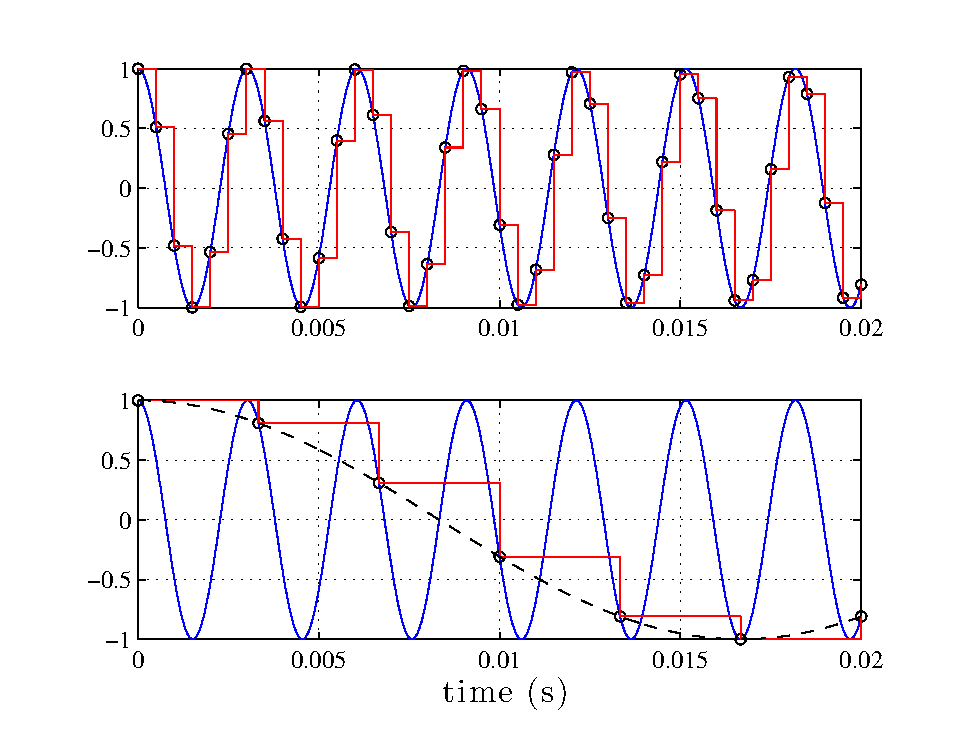
\includegraphics[width=\textwidth]{ch-computer/sampled}}
\caption[Sample and hold output]{Sample and hold
output. Analog input signal (sinusoidal curve) is a 330Hz sine wave; sampling
rate is 2000Hz (top) and 300 Hz (bottom). Output of S/H is red lines. Discrete value are shown as dark circles.\label{fg:sampled}}
\end{figure}

\index{analog-to-digital conversion!sampling|(}
A sample and hold (S/H) device acts like a switch and an analog memory device. While I may
talk of sampling a signal at a \emph{point} in time, a real device
requires a \emph{period} of time to perform its function, and this
includes sampling.  Over some short period of time, the S/H closes its
``switch'' and the analog signal is presented to the memory
device (which can be considered to be a capacitor, for example). The
memory device's internal voltage takes a short time to reach
equilibrium with the applied voltage --- called the \emph{aperture time}. After this aperture time,
the ``switch'' is opened and the sampled signal stays
stable while the ADC converts the signal to a digital value. However, the sampled signal 
doesn't stay perfectly constant --- some of the stored electrical
charge leaks away, and thus the sampled signal ``sags'' towards zero
volts.  While these limitations of the physical device are
important for sensor design and de-noising, we will focus on the basic idea of sampling at points in
time and assume the S/H performs like an ideal
device. Figure~\ref{fg:sampled} shows the input/output behavior of
such an idealized device.

%\begin{figure}
%\centerline{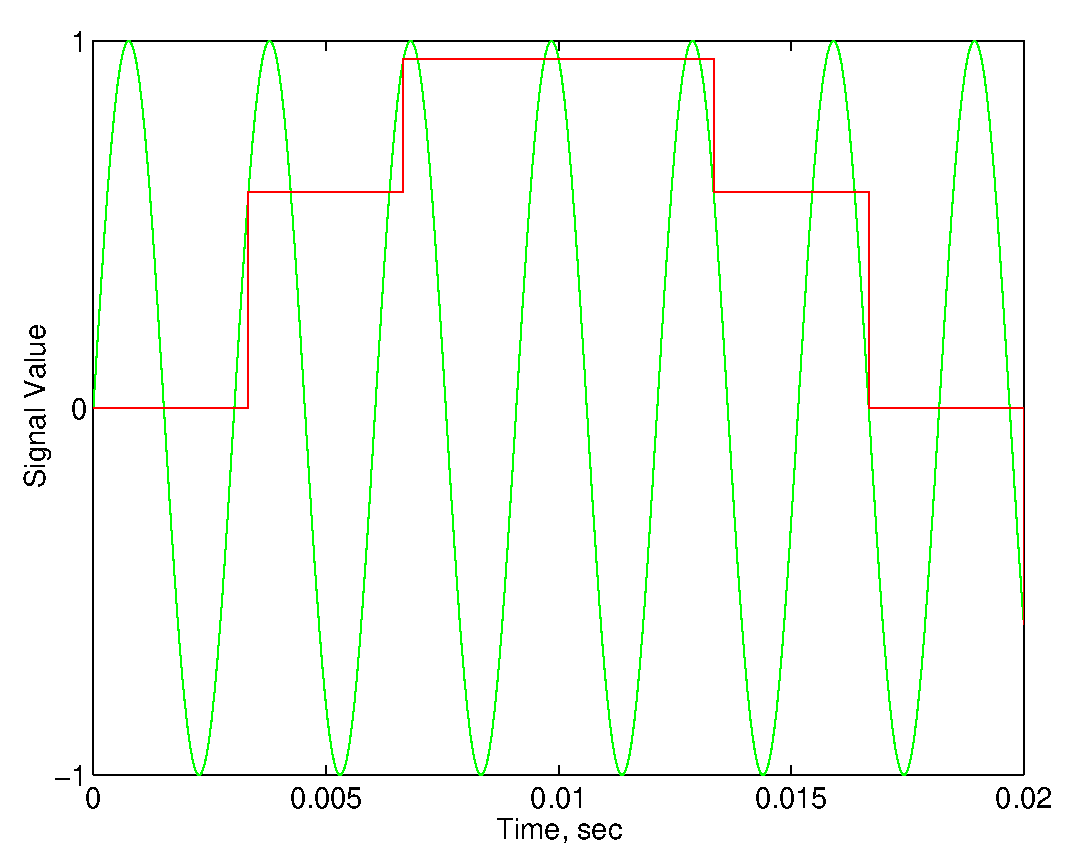
\includegraphics[width=\textwidth]{ch-computer/sampled_300}}
%\caption[Sample and hold output; 300Hzsampling rate]{Sample and hold
%output. Analog input signal (green) is a 330Hz sine wave; sampling
%rate is 300Hz. Output of S/H is plotted in red.\label{fg:sampled300}}
%\end{figure}

\index{Nyquist limit|see{analog-to-digital conversion, aliasing}}
\index{analog-to-digital conversion!aliasing|(}
We've already stated that we'd like the digitization process to retain
all the information in the original physical signal (or, at least,
that not being possible, to retain all information can be practically obtained).
However, sampling alone can destroy information. In the case of
figure~\ref{fg:sampled} (top), no information is lost (the original
waveform could in principle be reconstructed) because the sampling
rate, at 2000Hz, is much higher than the sinusoid's frequency, 330Hz.
Of course, the higher the sampling rate the more expensive the S/H and
ADC, and the more data produced at the output (i.e., a
higher data rate).  How slowly can we sample a sinusoid?
Figure~\ref{fg:sampled} (bottom) shows the same sinusoid, but this time sampled at 300Hz. In the 20ms
plotted, the original signal goes through approximately six cycles. If
we look at the sampled signal, it looks like a sampled version of a
sinusoid that goes through only a half cycle. If we reconstruct from the sampled signal and compared it to the original it would have an extremely low SNR! It
appears that the relatively low sampling rate has caused the 330Hz
frequency component of the original signal to appear as an
\emph{alias} at a lower frequency (perhaps 25 or 30 Hz).  

\subsection{Aliasing}
We see aliasing all the time in our everyday lives. For example, if you have ever seen video of a car wheel on the highway, it appears as though the wheel is spinning much slower than its actual rate. This is because the video camera is not sampling the wheel image fast enough and the high frequency spinning rate aliases back to a low frequency. 

Aliasing will occur for a sinusoid whenever the sampling rate is
less than twice the sinusoid's frequency.  Or, alternatively, given a
particular sampling rate, only sinusoids with frequencies up to
one-half that rate will be accurately represented. This cutoff
frequency is called the \emph{Nyquist frequency}. Let's suppose we
sample a phasor $x(t)$ every $T_s$ seconds. The original,
analog phasor is $x(t) = e^{j\omega_0 t}$. The sampled version of
the phasor is:
\begin{align}
x[n] & = x(\underbrace{n T_s}_{\stackrel{\text{sample}}{_\text{times}}}) \notag\\
     & = e^{j\omega_0 nT_s} \label{eq:samp-phasor}
\end{align}

In equation~(\ref{eq:samp-phasor}), $x[n]$ gives the value of the signal at the
sample times: the phasor represented as a sequence of measurements,
each taken at a time that is a multiple of the sampling interval
$T_s$. This was done by replacing $t$ by $nT_s$, the sampling times
($\{0, T_s, 2T_s, 3T_s, \ldots$). $x[n]$ is a \emph{discrete} signal
(a function of discrete time). For example, $x[n]$ could be the black circles in
figure~\ref{fg:sampled}. The value of $x[n]$ is undefined when $n$ is not an integer. 

The fundamental reason for aliasing is that we do not know what happens between samples. Take for example a continuous periodic signal. Every cycle of the signal repeats, so we can't tell if two
samples were taken from two successive cycles, or if a single cycle
was skipped in between them, or if a hundred cycles were
skipped. If we sample a signal and then reconstruct it from the samples we must assume that in between samples the signal is smooth (i.e., it has no other frequencies above the Nyquist frequency). 

To reconstruct a signal from its samples we need to talk about the notion of \emph{actual frequency} versus \emph{digital frequency} and \emph{apparent frequency}. We can use these quantities to calculate precisely if a frequency will alias, and at what frequency it will appear. The actual frequency of a signal is the continuous time frequency that we are accustomed to talking about. For  $e^{j\omega_0 t}$, the actual frequency is $\omega_0$. The digital frequency is the frequency at which the signal appears to be based on the indices, $n$, of the sampled signal. Once sampled, $ e^{j\omega_0 t}$ becomes $ e^{j\omega_0 nT_s}$ which has a digital frequency of $\hat{\omega}_0=\omega_0 T_s=\omega_0 \frac{2\pi}{\omega_s}$.  

\begin{align}
x(t) & = \exp(j\underbrace{\omega_0}_{\stackrel{}{\text{actual}}}t) \notag\\
x[n] & = \exp(j\underbrace{\omega_0 T_s}_{\stackrel{}{\text{digital, $\hat{\omega}$}}} n) \label{eq:samp-phasor-nyq}
\end{align}

Digital frequency, $\hat{\omega}$, \emph{must be} between $-\pi$ and $\pi$. This is because of Nyquist. For example, if the sampling rate, $\omega_s$, is equal to $4\omega_0$, then the digital frequency is
 \[
 \hat{\omega}_0=\omega_0 \times  \frac{2\pi}{\omega_s}=\omega_0\times \frac{2\pi}{4\omega_0}=\frac{\pi}{2} \notag 
 \]
which is less than $\pi$, so Nyquist is satisfied. Apparent frequency, $\omega'$, is the frequency at which we get by converting from digital frequency to continuous time frequency. To convert from digital frequency to apparent we use the following formula,

\begin{equation}
\omega' = \hat{\omega}\times \frac{\omega_s}{2\pi} \label{eq:conv-dig-app}
\end{equation}

For our continuing example, when $\omega_s$ is equal to $4\omega_0$, this means the apparent frequency is $\omega'_0=\pi/2\times \frac{\omega_s}{2\pi}=\pi/2\times \frac{4\omega_0}{2\pi}=\omega_0$. Since the cosine was sampled greater than the Nyquist rate, the apparent frequency equals the actual frequency. 

If we sample at a frequency less than Nyquist the apparent and actual frequencies are different. For example, if we instead sample at $\omega_s=4/3\omega_0$, then the digital frequency will be $\hat{\omega_0}=\omega_0 \frac{2\pi}{4/3\omega_0}=3\pi/2$, which is not on the interval  $-\pi$ to $\pi$. We convert the frequency down by using a clever identity, $e^{-j2\pi n}$, which is equal to 1 for all values of $n$,

\begin{align}
x[n] & = e^{j \frac{3\pi}{2}n} \notag\\
  & = e^{j \frac{3\pi}{2}n} e^{-j2\pi n} && (e^{-j2\pi n}=1)\notag\\
  & = e^{j (\frac{3\pi}{2} -2\pi)n} && (\text{combine exponents})\notag\\
  & = e^{-j \frac{\pi}{2}n} && (\text{equivalent digital frequency}) \notag
\end{align}
%
Essentially, this identity allows us to subtract $2\pi$ from the digital frequency until it is on the correct interval. Digitally, we see that  $\frac{3\pi}{2}$ is the same as $-\frac{\pi}{2}$. When we convert to apparent frequency we get $\omega'_0=-\pi/2\times \frac{\omega_s}{2\pi}=-\pi/2\times \frac{4\omega_0}{6\pi}=-\omega_0/3$, which is lesser in magnitude than the actual frequency and negative (the phasor is spinning in the opposite direction).

Furthermore, from equation~\ref{eq:conv-dig-app} we can see that the sampling frequency, $\omega_s$, corresponds to the digital frequency $\hat{\omega}=2\pi$. In digital frequency, we have seen that all frequencies at multiples of $2\pi$ from each other have the same apparent frequency. This gives the following relationship between apparent and actual frequency:
 \begin{align}
 \omega'_0 =&\omega_0 + k \omega_s && (k = \ldots, -2, -1, 0, 1, 2, \ldots)
 \end{align}
The apparent frequency could be the result of any frequency that is at a multiple of the sampling frequency. 

%When we sample a function $x(t)$, we get an array $x[n]$ that has no time information (only an index, $n$). Let's assume we sample a signal at a frequency of $\omega_s=2\pi/T_s$ and the signal is a cosine wave at a frequency $\omega_0=\omega_s/4$ (the \emph{actual} frequency is $\omega_0$ and is one fourth the sampling frequency). We know from \ref{eq:samp-phasor} that the discrete signal will be $ \cos{\omega_0 nT_s}$. 
%
%%\begin{align}
%x[n] & = \cos{\omega_0 nT_s}
%     \label{eq:samp-phasor-nyq}
%\end{align}
% 
%Let's explore this in more detail by purposefully sampling
%the signal at too low of a rate. That means that, after sample
%$x[n-1]$ is taken, the next sample --- $x[n]$ --- will be taken some
%number of cycles later. Call the number of cycles between the two
%samples $k$. Clearly, $x[n+1]$ will then occur $k$ cycles after
%$x[n]$, and so on. Since the period of the signal is $2 \pi/\omega_0$,
%we can write the sampling interval as $T'_s = (T_s + k 2
%\pi/\omega_0)$, where $T'_s$ is the sampling interval written to show
%explicitly that it is greater than one cycle of the sinusoid. As in
%equation~(\ref{eq:samp-phasor}), we can write the sampled signal as:
%\begin{align}
%x[n] & = e^{j\omega_0 nT_s} \notag\\
%     &= e^{j\omega_0 nT_s} && \omega_0 = 2/3\omega_s \\
%     &= e^{j2/3\omega_s  nT_s} \\
%x[n] & = e^{j\omega_0 nT'_s} \notag\\
%     & = e^{j\omega_0 n(T_s + k 2 \pi/\omega_0)}
%     &&\text{(substitute expression for cycle skipping, $T'_s$)}
%     \notag\\
%     & = e^{jnT_s(\omega_0 + k 2 \pi/T_s)}
%     &&\text{(factor out $T_s$)}
%     \notag\\
%     & = e^{j\omega'_0 nT_s}
%     &&\text{(where we've called $\omega'_0=\omega_0 + k 2 \pi/T_s$)}
%\label{eq:samp-phasor2}
%\end{align}
%
%By rearranging the terms as in equation~(\ref{eq:samp-phasor2}), we
%see that sampling at too low a rate means that the discrete signal
%$x[n]$ can be interpreted as a phasor with frequency $\omega'_0 =
%\omega_0 + k 2 \pi/T_s$, $k = \ldots, -2, -1, 0, 1, 2, \ldots$.

Now, remember that we are dealing with a real-valued signal, not a
complex-valued one; we use the complex exponential as a representation
that makes the math easier. For a real-valued signal, the imaginary
component of the complex exponential must be canceled out. We can do
this easily by adding another complex exponential at a negative
frequency, since $\cos \omega_0t = 1/2 e^{j\omega_0t} + 1/2
e^{-j\omega_0t}$. So, for a completely real sinusoid we should really write,
\begin{align}
\{\omega'_0\} &= \pm\omega_0 + k\omega_s
\label{eq:set-ambig-freq}
\end{align}

Let's consider the case where $\omega_s/2 < |\omega_0| < \omega_s$,
that is, the sinusoid's frequency is just a bit greater than the
Nyquist frequency (or, alternatively, you could think of it as the
sampling rate being just a bit too slow: $\omega_s <
2|\omega_0|$). Call the amount that $|\omega_0|$ exceeds $\omega_s/2$
by $\omega_a = |\omega_0| - \omega_s/2$.  Let's figure out what
happens to the negative frequency component, $-\omega_0$. Using
$\omega_a$, we can rewrite $-\omega_0$ as 
\begin{equation}
-\omega_0 = -\omega_a - \omega_s/2
\label{eq:neg-freq}
\end{equation}
(this is simply solving the $\omega_a$ equation for $-\omega_0$).

But we know that, according to equation~(\ref{eq:set-ambig-freq}), the
sinusoid's frequency really corresponds to a set of ambiguous
frequencies, and so we can write equation~(\ref{eq:neg-freq}) as
$-\omega_0 + k\omega_s = -\omega_a - \omega_s/2 + k\omega_s$ to show
\emph{all} of the ambiguous frequencies. To simplify matters, let's
just look at the ``first'' ambiguous frequency at $k=1$:
\begin{align*}
\omega'_0 &= -\omega_a- \omega_s/2 + k\omega_s && (\text{substitute $k=1$}) \\
\underbrace{\omega'_0}_{\stackrel{\text{apparent}}{_\text{ frequency}}} &= - \omega_a +
     \underbrace{\omega_s/2}_{\stackrel{\text{Nyquist}}{_\text{ frequency}}}
\end{align*}

So, the apparent frequency is one that is just a bit below the Nyquist
frequency. In fact, if we substitute back in the definition of
$\omega_a$, we get that the apparent frequency is located at $\omega_s
- \omega_0$. So, the first ambiguous frequency for the negative
frequency component of a real sinusoid is located at a positive
frequency.

What if the sampling frequency is not just a bit too slow? In that
case, $\omega_0 > \omega_s$. To find the location of the $k=1$
ambiguous frequency, we can follow the above procedure and find that
we can just subtract multiples of $\omega_s$ from $\omega_0$ until its
absolute value is less than $\omega_s/2$.  Now we can see that the
sampled signal in figure~\ref{fg:sampled} (bottom) must have a frequency of
330-300=30Hz (subtracting the sampling frequency of 300Hz from the
sinusoid's frequency of 330Hz one time).

At the end of chapter~\ref{ch:physical-signals}, we saw how
\emph{any} function can be represented as a sum of sinusoids --- its
Fourier series. If you look at the above discussion, you will see
that, if we replace the phasor in, say,
equation~(\ref{eq:samp-phasor-nyq}) by a sum of phasors at frequencies
$\omega_1, \omega_2, \omega_3, \ldots$, we will reach the same
conclusions, but they will now apply to \emph{each frequency
  component}: each will produce aliases. In the case of the square
wave of Figure~\ref{fig:fs-pulse}, the frequencies of the sinusoids
have no upper limit --- the signal's \emph{spectrum} is infinite.
Certainly, then, there will be frequencies greater than $\omega_s/2$,
regardless of how fast we sample.

How can we avoid this aliasing? We've been discussing the Nyquist
frequency in terms of the sampling frequency; that the signal must
have frequency components less than one-half the sampling frequency.
Another way of looking at sampling is to require that the input signal
be \emph{band limited}: that it have a maximum frequency component,
rather than an infinite spectrum. Given that the signal is band
limited with maximum frequency $\omega_m$ (which we can achieve using
\emph{filters}, as described in chapters~\ref{ch:filt-intro}
and~\ref{ch:fb-filters}), then we can set our sampling rate so that it
is at least $2\omega_m$.
\index{analog-to-digital conversion!aliasing|)}

\problemset{
\subsection*{Self-Test Exercises}

See~\ref{sc:ch2ex} \#\ref{it:ch2ex1}--\ref{it:ch2ex3} for answers.

\begin{enumerate}
\item Aliasing can happen in the world around you. Identify the source
  of the original signal and the sampling mechanism in the following
  situations:
\begin{enumerate}
\item The hubcap of a car coming to a stop in a motion picture;
\item A TV news anchor squirming while wearing a tweed jacket;
\item A helicopter blade while the helicopter is starting up on a
  sunny day.
\end{enumerate}
\end{enumerate}
\index{analog-to-digital conversion!sampling|)}}


\section{Quantization}

\index{analog-to-digital conversion!quantization|(}
Understanding aliasing helps us deal with the problems raised by \emph{discretizing time} using
a sample and hold device. There is another discretization that occurs,
however: a discretization of the \emph{analog level} output from the S/H to
the finite number of binary values output by the ADC. This process is
formally known as \emph{quantization}. Since an ideal analog signal
has an infinite number of possible values, while the computer
representation (be it integer or floating point) has a finite number
of values, there will be some error.

\begin{figure}
\centerline{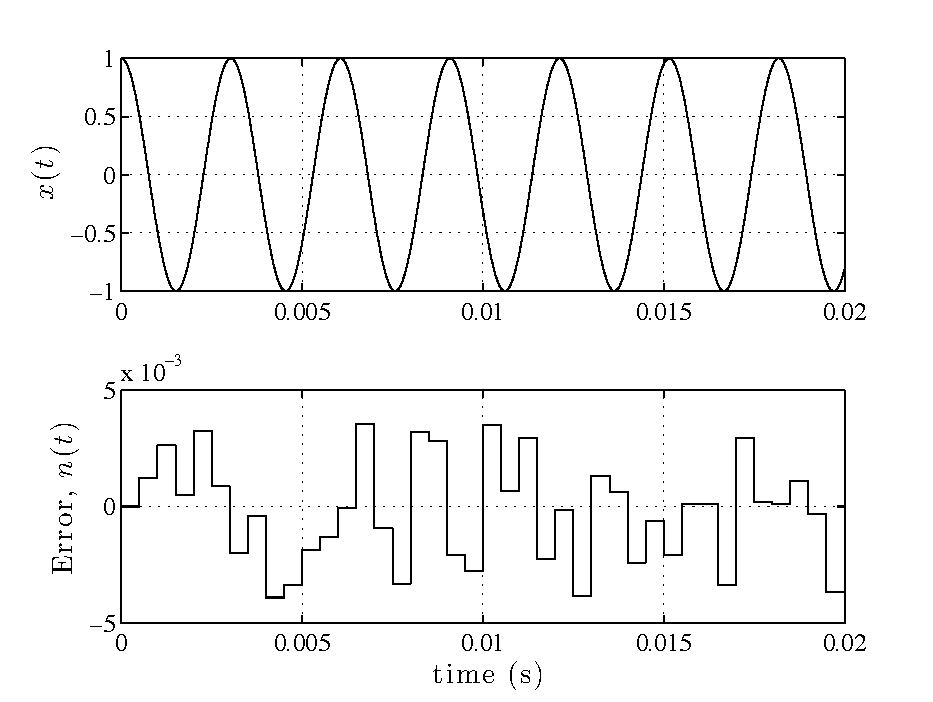
\includegraphics[width=\textwidth]{ch-computer/quant-error_2000}}
\caption[Error in output for 8-bit ADC]{Error in output (bottom) of an
ADC that uses 8 bits to represent values in the range [-1, +1] for the
S/H output in figure~\protect\ref{fg:sampled} (top). Original analog
signal is shown in top plot.\label{fg:quant2k}}
\end{figure}

This error is illustrated in figure~\ref{fg:quant2k}. To produce this
figure, the output of the S/H from figure~\ref{fg:sampled} (top) was
quantized to 256 levels, each corresponding to 1/256 of the distance
between -1 and +1. This result was then subtracted from the ideal S/H
output and plotted as the error shown in the bottom plot in the
figure. How much can this error be? The error can be as much as one
part in $\pm 1/2$ of the least significant bit  (LSB). In other words, the S/H signal is within LSB/2 of the
actual signal. What are the statistics of this noise? Assuming that Nature hasn't
conspired against us, we would expect the mean of this error to be
zero.  If all ADC input values have equal probability, then the errors
should also, which means that it is uniformly distributed between
minus and plus one-half.  Remembering our statistics, the standard
deviation of a continuous random variable is the square root of its
variance,
\begin{equation}
\sigma^2 = \int_{-\infty}^{+\infty} (x-\mu)^2 \mathrm{d}x
\label{eq:var}
\end{equation}

In this case, $\mu=0$ and the variable's range is [-1/2, +1/2]. The
result is a standard deviation of $\sigma = 1/\sqrt{12} \,
\mathrm{LSB} \approx 0.29
\, \mathrm{LSB}$ (how [answer in~\ref{sc:ch2ex}
\#\ref{it:ch2ex4}]?). In the case of an 8-bit ADC, this
comes to 0.29/256 = 1/883 of the ADC's full range.

\index{analog-to-digital conversion!quantization!noise|(}
Noise is ubiquitous in the physical world --- and this includes
analog electronics (digital electronics have noise, too, but its
effect on digital signals is different). Sometimes, this noise is
truly random, or \emph{stochastic}, perhaps produced by thermal
effects within the circuitry. Other times, the noise is merely
unwanted signal, such as ``background noise'' in an audio recording.
To quantify this noise we will use SNR (equation \ref{eq:SNR}). The standard deviation, $\sigma$, is an estimate of the noise power ($n_{RMS}=\sigma$). For simplicity we will assume that the signal uses the entire ADC range (256 levels, $x_{RMS}=256$).
%Noise is usually quantified as a ratio --- \emph{signal-to-noise
%ratio}, or SNR --- and expressed in decibels (a logarithmic scale). To
%convert a ratio of two magnitudes
%$R_M=\mathrm{Mag}(\mathrm{signal})/\mathrm{Mag}(\mathrm{noise})$ to
%decibels, we calculate
%$\mathrm{SNR_{dB}} = 20 \log_{10}{R_M}$. (If we were talking about a
%ratio of powers $R_P$, it would be $\mathrm{SNR_{dB}} = 10
%\log_{10}{R_P}$.) 
So, for example, if there was no other noise
present than that from quantization by an 8-bit ADC, the SNR would be
$20 \log_{10} 256/0.29 \approx 59\mathrm{dB}$. For a 12-bit ADC, the SNR is
83dB; for 16-bit, the SNR is 107dB.

Let's suppose that the ADC input signal has a range of 5 volts (V),
and that it includes noise (from whatever source) with a standard
deviation of 1 millivolt (mV). If we use an 8-bit ADC, 5V corresponds
to 255 and 1mV is then 0.051 LSB. (What is the SNR for the original
signal (answer in~\ref{sc:ch2ex} \#\ref{it:ch2ex5}) ? 

When we add
random variables, we add their variances, and so the standard
deviation of their sum is the square root of the sum of their
variances, $\sigma' = \sqrt{\sigma_1^2 + \sigma_2^2}$. For an 8-bit
ADC, then, we have the total noise (inherent plus quantization) of
$\sqrt{0.051^2 + 0.29^2} = 0.294 \, \textrm{LSB}$. So, almost all of
the noise in the digitized signal is caused by quantization (the noise
on the output represents a 476\% increase from the input noise)! If we
go to 12 bits, the total noise is $\sqrt{0.82^2 + 0.29^2} = 0.87 \,
\textrm{LSB}$ --- quantization increases the noise by 6\%. From a
design point of view, we \emph{select} the ADC based in part on the
expected noise in the analog signal and the maximum noise we can
tolerate in the digital one.  \index{analog-to-digital
  conversion!quantization!noise|)}

\problemset{
\subsubsection*{MATLAB and Sound Files}
\begin{sloppypar}
\begin{itemize}
\item A MATLAB .m file for demonstrating quantization using tones is available
at \url{http://courses.washington.edu/css457/ebook/quantdemo1.m}.
\index{MATLAB code!quantization}
\item A MATLAB .m file for demonstrating quantization using a more
interesting sound is available at
\url{http://courses.washington.edu/css457/ebook/quantdemo2.m},
\index{MATLAB code!quantization}
along with a data file at
\url{http://courses.washington.edu/css457/ebook/amoriole2.mat}.
\index{audio files!bird calls}
\end{itemize}
\end{sloppypar}}

\problemset{
\subsection*{Self-Test Exercises}

See~\ref{sc:ch2ex} \#\ref{it:ch2ex6} for the answer.

\begin{enumerate}
\item What ratio of amplitudes is represented by one bel?
\end{enumerate}
\index{analog-to-digital conversion!quantization|)}}

\section{Dynamic Range}

\index{analog-to-digital conversion!dynamic range|(}
So, one reason we might choose an ADC with more bits is to reduce the
effects of quantization noise.  There is another reason: our desire to
represent both low and high amplitude signals with reasonable
fidelity. The need for this \emph{dynamic range} can result in us
needing more bits.  Let's use as an example the digitization of an
orchestra where the ratio of the low amplitude passages to the high
amplitude ones is 1/1000 (60dB).  If we use an 8-bit ADC, then 255
corresponds to the highest amplitude and the lowest amplitude is 0.255
LSB. In other words, we have used just about all the bits for the
loudest passages, leaving nothing for the quiet parts!  For a 12-bit
ADC, the lowest amplitudes are allocated about 2 bits; for a 16-bit
ADC, only about 6 bits. The reason for this is that we've coded the
signal \emph{linearly}, with the step between ADC outputs being the
same for low and high amplitude signals. Logically, however, it would
seem unlikely that our ears would be as sensitive to slight changes in
loud passages as they would be to the same changes to quiet ones.

This intuition is correct, and so consideration of the
\emph{psychophysics} of hearing (the intersection of the physics of
sound and the psychology of perception) leads us to a solution for
\index{perception!auditory!psychophysics}
audio digitization: \emph{companding}. 
\index{companding}
We first pass the analog signal through a ``squashing function''
before digitization. This nonlinear function doesn't modify the quiet
passages (the region of the function near zero is basically linear,
with a slope of one).  However, it causes changes in loud passages to
result in smaller changes in the signal to be digitized. This is
equivalent to allocating more bits to the quiet passages and fewer to
the loud ones. Assuming we use the exact inverse function on any audio
output provided by our system, there should be little noticeable
effect of this companding.

Of course, this is all based on the assumption that we are digitizing
a signal that will be listened to. If, on the other hand, the signal
is some other kind of data not for ``human consumption,'' then small
steps at high amplitude may be just as important as those at low ones,
and so companding won't be usable --- it would destroy valuable
information.
\index{analog-to-digital conversion!dynamic range|)}
\index{analog-to-digital conversion|)}

\section{Periodic and Aperiodic Signals}

In this chapter, we talked about a signal as being a sum of sinusoids,
as in chapter~\ref{ch:physical-signals}. In general, a periodic
signal can be expressed as a sum of \emph{both} sines and cosines,
which we can express as the sum of complex sinusoids:
\begin{equation}
f(t) = \sum_{k=-\infty}^{+\infty} c_k e^{jk 2\pi t/T}
\label{eq:fseries}
\end{equation}

Equation~(\ref{eq:fseries}) is the general Fourier series, which can
be used to represent any periodic signal with period $T$. In this
series, all of the complex sinusoids have periods that are multiples
of $T$ (frequencies that are multiples of $2\pi/T$). So, the frequency
content, or \emph{spectrum}, of a periodic signal (the $c_k$s) is
\emph{discrete}: it only has values at particular frequencies.

As we shall see in chapter~\ref{ch:fft}, for an aperiodic signal, the
Fourier series becomes the \emph{Fourier integral}, and the signal's
spectrum is \emph{continuous}:
\begin{equation}
f(t) = \frac{1}{2\pi} \int_{-\infty}^{+\infty} F(j\omega)
                          e^{j\omega t} \mathrm{d}\omega
\label{eq:fint}
\end{equation}

In equation~(\ref{eq:fint}), the function $F(j\omega)$ describes the
magnitude of the complex sinusoid at frequency $\omega$.  This is the
continuous (because $\omega$ can take on all values, not just a
discrete set) spectrum of an aperiodic signal. Intuitively, we take the limit as the period of the signal goes to infinity in equation~\ref{eq:fseries}, which pushes the spacing between the $c_k$ spectral lines closer and closer until the spectrum becomes continuous. I'll revisit this
topic later, in more detail.

\section{Problems}

%\begin{enumerate}
%\item The analytical formula for synthesis of a 50\% duty cycle square
%  wave as a sum of harmonically related sine waves (its Fourier
%  series) is:
%  \begin{equation*}
%    x(t) = \frac{4}{\pi} \left( \sin(\omega_0 t)
%      + \frac{1}{3} \sin(3\omega_0 t)
%      + \frac{1}{5} \sin(5\omega_0 t) + \cdots \right)
%  \end{equation*}
%  Write a MATLAB program to compute and plot the spectrum of a square
%  wave given this equation.  Your program should prompt the user for
%  $\omega_0$ and which harmonic is the maximum to plot. Note that you
%  are \emph{not} being asked to plot the square wave as a function of
%  time; you should plot the amplitudes of the component sinusoids as a
%  function of the sinusoids' frequencies (like
%  figure~\ref{fig:fs-pulsecn}). Hand in hard copy of your MATLAB code
%  and a plot of the spectrum with 10 harmonics. You may find the
%  MATLAB function \texttt{stem()} useful.\label{it:sq-wave-spectrum}
%
%\item Modify your above program to show how these harmonics are
%  aliased if the square wave is sampled at $\omega_s$ (prompting the
%  user for $\omega_s$). Hand in hard copy of your code and an example
%  plot for $\omega_s < \omega_0$.\label{it:aliased-sq-wave}
%
%\item Modify your program to play the sound of the aliased square wave
%  (synthesize $x(t)$ from problem~\ref{it:aliased-sq-wave}). Next,
%  write a program to generate a band-limited square wave from a sum of
%  sinusoids, given $\omega_0$ and $\omega_s$, with no frequency
%  components above the Nyquist limit. Play that sound (the MATLAB
%  function \texttt{soundsc()} is useful for this). Compare the sounds
%  with and without (from problem~\ref{it:sq-wave-spectrum}, given that
%  $\omega_s$ determines $\omega_\mathit{max}$) aliasing. Can you find
%  an interesting use for intentional aliasing? Hand in your code's
%  hard copy, plots of the sample square wave and the band limited
%  square wave (as functions of \emph{time}), and your written
%  comments.
%\end{enumerate}

\begin{enumerate}

\item What is the RMS magnitude of the sine wave $A\sin(\omega t)$?
			%answer: A/sqrt(2)
\item What is the RMS magnitude of the sawtooth waveform 
\begin{equation*}
			x(t) = \frac{A}{T} t\text{,        } 0<t<=T
\end{equation*}
			where $x(t)$ repeats every $T$ seconds
			%answer: A/sqrt(3)
\item The sin wave from problem 1 is sampled in noise, 
			if the desired SNR is 20 dB, how large can the RMS magnitude of the noise be?
			%answer: 20 = 20 log(A/(sqrt(2) Nrms)), Nrms=A/(sqrt(2)*exp(1))
\item If the sawtooth waveform from problem 2 is considered noise and
			the sine wave from problem 1 is the signal, what is the SNR in dB?
			%answer: 10 log(sqrt(3/2))=5 log(3/2)=0.9dB
\item The signal $e^{j 2\pi \times200 t}$ is sampled at $\omega_s=2\pi\times300$. 
			What are the actual, digital, and apparent frequencies?
			% answer: 2pi*200rad/s, -2/3 pi rad/sample, -100 *2pi rad/s
\item The signal $\cos( 2\pi \times200 t)$ is sampled at $\omega_s=2\pi\times250$.
			What are the actual, digital and apparent frequencies of the resulting cosines?
			%answer: 2pi*200rad/s, 2/5 pi rad/sample, 50 *2pi rad/s
\item Consider the 50\% duty cycle square wave with amplitude from -1 to 1 and period $T$.
\begin{enumerate}
\item What is the RMS magnitude?
\item The fourier series of the 50\% duty cycle square wave is given by,
\begin{equation*}
\frac{4}{\pi} \sum_{k=1,3,5...}^\infty \frac{\sin(k \omega_0 t)}{k}
\end{equation*}			
If we consider the ``band limit'' of the square wave to be when it has no other frequencies with magnitudes larger than 1\% of the RMS magnitude, then what is the minimum sampling rate to capture all frequencies below the ``band limit'' without aliasing?
	\end{enumerate}
\item Suppose we wish to sample from an audio signal that ranges from 0 to 2.5V (Assume that the range of our ADC is 0-2.5V also). If the analog noise on the line is 3mV and our ADC is 8bits, what percentage of the total SNR is from the analog noise and what percentage is from the 8 bit quantization?
\item If we have the same signal from question 8 (audio signal from 0-2.5V with 3mV analog noise), 
	\begin{enumerate}
			\item how many bits should our ADC have so that the noise added by quantization is less than the analog noise?
			\item how many bits should our ADC have so that the quantization noise does not decrease our SNR by more than 1\%?
	\end{enumerate}

\end{enumerate}

\section{Further Reading}

James H McClellan, Ronald W. Schafer, and Mark A. Yoder, \textit{DSP
  First: A Multimedia Approach}, Prentice Hall, 1998, chapter 4 (\S
4.1--4.3).

% LocalWords:  phasors

% -*-LaTeX-*-

% The log below is the old log from when RCS was being used in
% conjunction with this.
%
% $Log: filt-intro.tex,v $
% Revision 1.7  2007/12/11 02:10:08  stiber
% All the relatively small modifications for the start of the
% Winter 2008 quarter.
%
% Revision 1.6  2007/03/20 23:52:45  stiber
% Cleaned up and updated LaTeX.
%
% Revision 1.5  2007/03/18 18:56:10  stiber
% Modified file for stand-alone textbook. Checked that it will format
% along with the rest of the book as of this point.
%
% Revision 1.4  2006/03/27 23:36:06  stiber
% Fixed error in formula.
%
% Revision 1.3  2004/05/03 20:13:30  stiber
% Fixed typos and errors in end of chapter problems.
%
% Revision 1.2  2004/03/29 19:53:17  stiber
% Updated for Spring 2004 and new textbook (DSP First).
%
% Revision 1.1  2004/02/19 00:24:08  stiber
% Initial revision
%

\chapter{Filtering and Feedforward Filters}
\label{ch:filt-intro}

% Use the starred versions of section, subsection, etc.
\section{Introduction}

In this chapter, we will introduce you to the most basic type of
algorithm for processing digital signals: feedforward filters. We
start with the concept of \emph{filtering} and the operation of basic
feedforward filters. By the end, you should understand some important
terms related to filters, for example, \emph{frequency response},
\emph{phase response}, \emph{transfer function} and \emph{zeros} of a
\emph{transfer function}. You should be able to implement simple
digital filters on a computer and use them to solve some simple signal
processing problems.

The concept of filtering should not be new to you. For example, if you
were interested in filtering and opened this book, you would see that
this chapter deals with filtering and so you would pay attention to
this chapter and ignore the others.  Your mind performed a
\emph{bandpass} filter with the pass \index{filter!bandpass} band
being chapter \ref{ch:filt-intro}.  Some other kinds of filters are
\emph{low pass}, \emph{high pass}, and \emph{band stop}.  Using the
same example, a low pass filter \index{filter!low pass} allows you to
attend to all the chapters in the book, from the beginning to the end
of the pass band, say chapter~\ref{ch:filt-intro}; the high pass on
\index{filter!high pass} the other hand will pass only the chapters
beyond a certain one, say beyond chapter 4; the band stop is the one
\index{filter!band stop} that allows you to pay attention to all the
chapters \emph{except} the stop band, say chapter \ref{ch:filt-intro}.

In the signal processing domain, filters exclude and/or include signal
\emph{frequencies}. For example, consider a signal $x(t)$ (where $t$
is time) with four sinusoidal components. It has frequencies at
$f_1=50$, $f_2=100$, $f_3=250$, and $f_4=350$:

\begin{equation}
x=\sin(2\pi t f_1)+\sin(2\pi t f_2)+\sin(2\pi t f_3)+\sin(2\pi t f_4)
\label{eq:sine4}
\end{equation} 

\problemset{
\subsubsection{Self-Test Exercise}

See~\ref{sc:ch3ex} \#\ref{it:ch3ex0} for the answer.

\begin{enumerate}
\item Is the signal of equation~\ref{eq:sine4} periodic? If so, what
  is its period?
\end{enumerate}}

\begin{figure}
\centerline{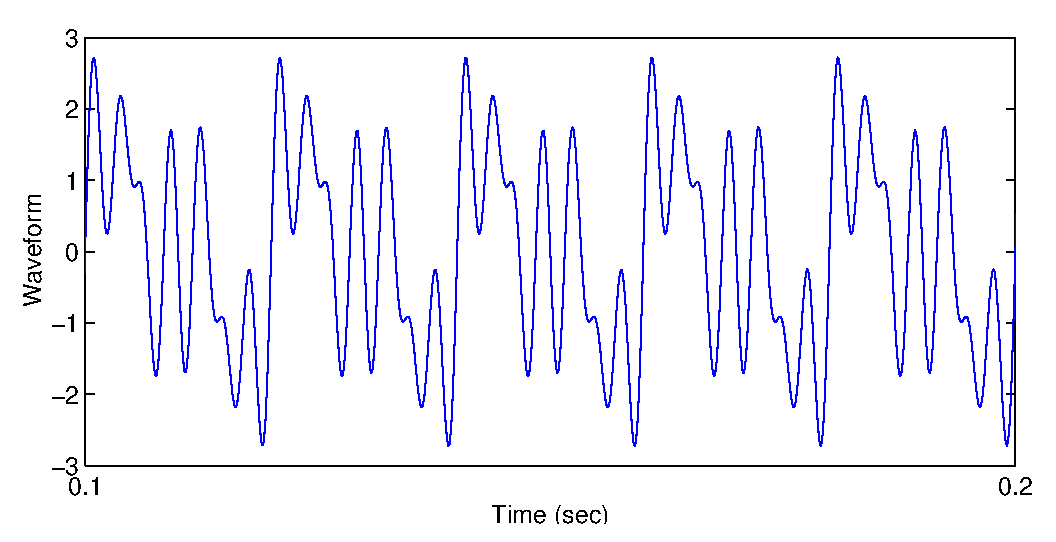
\includegraphics[width=5in]{ch-fir/sine4}}
\caption[Four frequency components]{A sinusoidal signal with four
frequency components: $f_1=50$, $f_2=100$, $f_3=250$,
$f_4=350$Hz.\label{fig:sine4}}
\end{figure}

Figure~\ref{fig:sine4} shows a plot of about 0.1 second of this
signal. Its four frequencies are shown as green peaks in
figure~\ref{fig:sine4-sp}.  Let's say that we would like to have a
filter to keep the $f_3=250$Hz sinusoid and get rid of the $f_1$,
$f_2$, and $f_4$ sinusoids. This filter can be visualized as in
figure~\ref{fig:sine4-band}. Here, the horizontal axis is frequency
and the vertical axis is magnitude of the filter's response. The
filter is designed to have a frequency passband between 200 and 300
Hz, which means that only the signal's frequency components within
this band are allowed to pass. Figure~\ref{fig:sine4-f2} shows this
filter's output --- in other words, the filtered signal --- plotted
along time. Another way to look at the filtered signal is its
frequency components, which are shown in figure~\ref{fig:sine4-sp}
(magenta). This latter graph clearly shows that, after filtering, the
signal is very close to a 250 Hz sinusoid, exactly as expected.  You
can hear these two signals as sounds:
\url{http://courses.washington.edu/css457/ebook/sine4.au} is the sum
of four sinusoids and
\url{http://courses.washington.edu/css457/ebook/filtered_sine4.au} is
the filtered version.  \index{audio files!sinusoids} \index{audio
  files!filtering}

\begin{figure}
\centerline{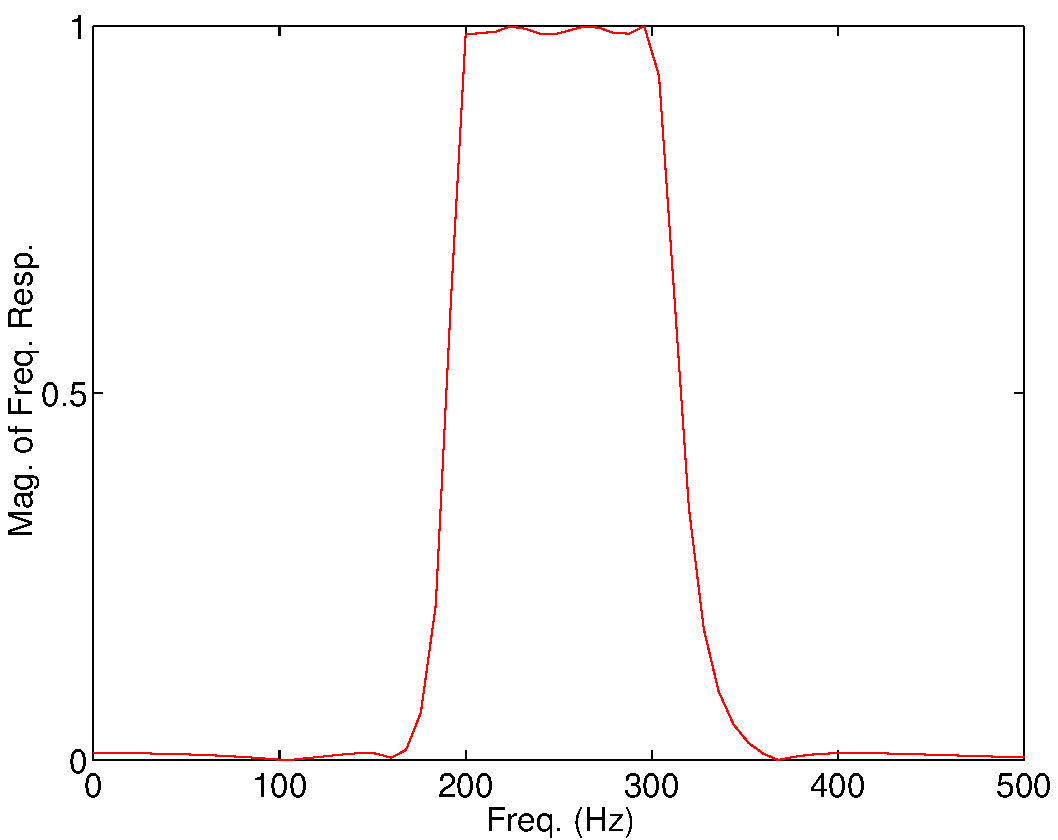
\includegraphics[height=3in]{ch-fir/sine4_band200-300}}
\caption[Filter frequency response]{Filter's frequency response. The
pass band is [200 300] Hz.\label{fig:sine4-band}}
\end{figure}

\begin{figure}
\centerline{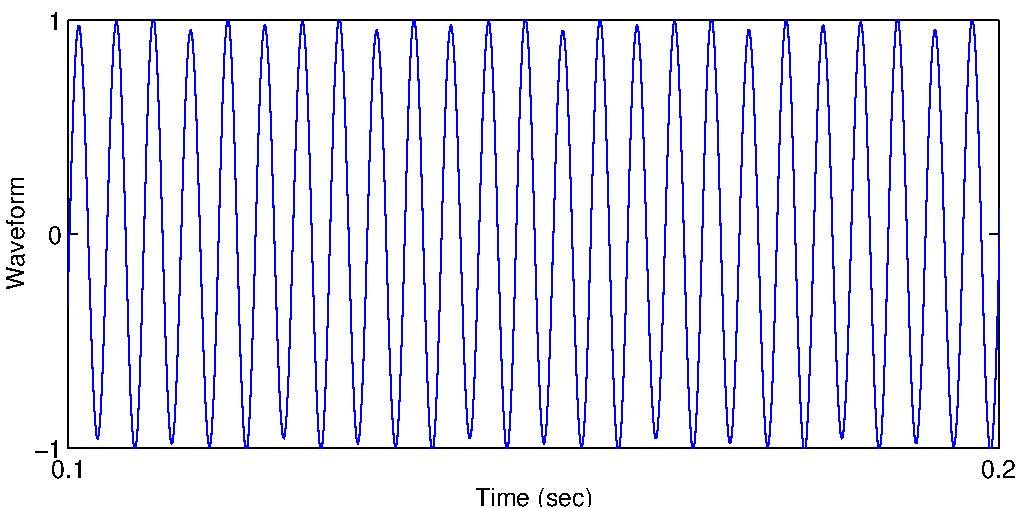
\includegraphics[width=5in]{ch-fir/sine4_filted}}
\caption[A filtered signal]{The signal~(\protect\ref{eq:sine4}) after filtering out
frequencies 50, 100 and 350Hz.\label{fig:sine4-f2}}
\end{figure}

\begin{figure}
\centerline{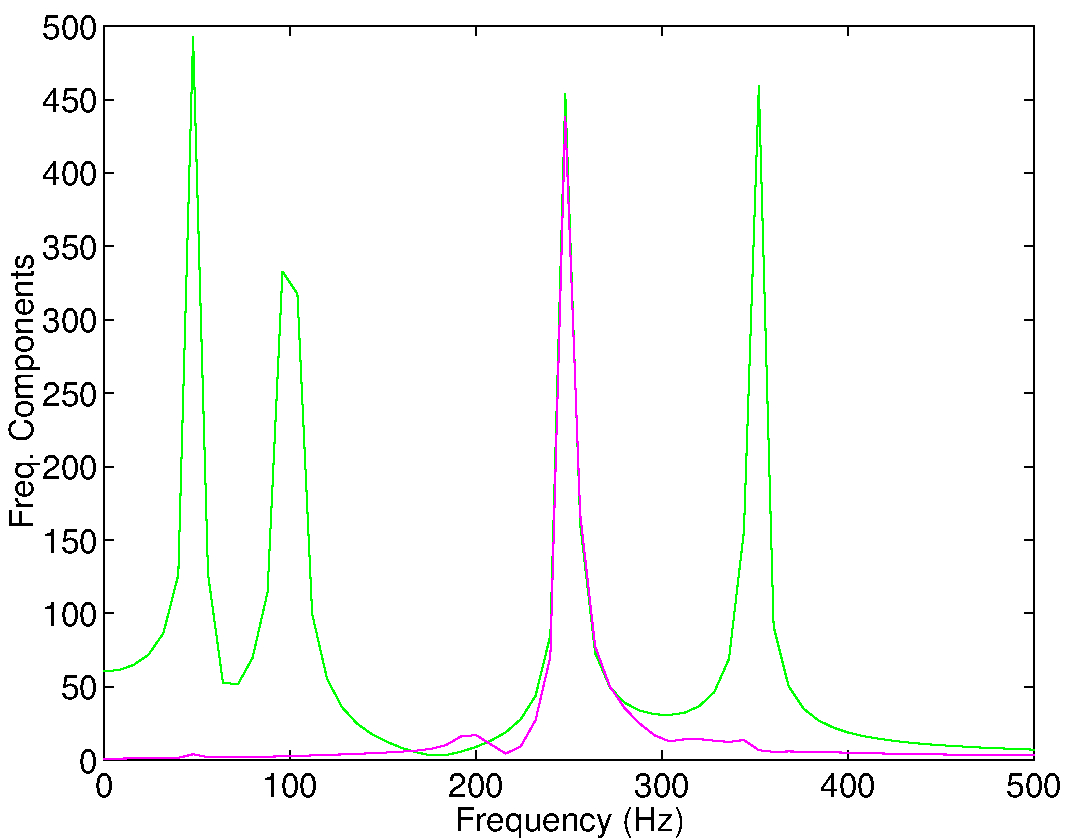
\includegraphics[height=3.5in]{ch-fir/sine4_sp}}
\caption[Unfiltered vs. filtered signal]{Spectrum of four-sinusoid
signal (green) and its filtered version
(magenta).\label{fig:sine4-sp}}
\end{figure}

At this point, you should have an idea of what filters do. Next, I
will explain \emph{how} filters work.

\section{Feedforward Filters}

\subsection{Delaying a phasor}

In chapter~\ref{ch:physical-signals}, we learned the term
\emph{phasor}, a complex sinusoid expressed as $e^{j\omega t}$.  We
also saw that this representation makes the math simpler for adding
sinusoids, at least.  A phasor's magnitude is one, its frequency is
$\omega$, and it angle is $\omega t$, where $t$ is time. It moves
around the unit circle counter-clockwise along time.  If we delay it
by $\tau$ sec, then the delayed time is $t-\tau$, and we can write
this as:

\begin{equation}
e^{j\omega (t-\tau)} = e^{-j\omega \tau} e^{j\omega t}
\end{equation}

This is the product of two phasors at the same frequency.
This doesn't do anything except rotate the phasor by $-\omega \tau$
(i.e., it doesn't change its magnitude).

\subsection{A simple feedforward filter}

\begin{figure}
\centerline{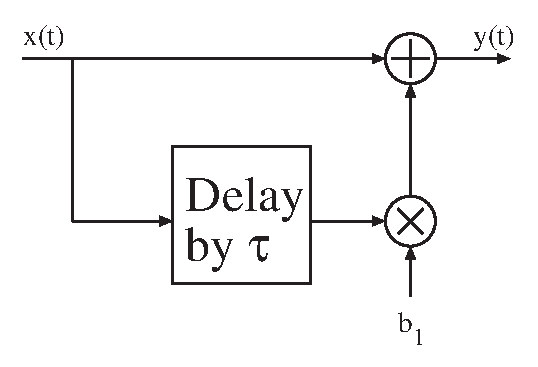
\includegraphics[width=0.5\textwidth]{ch-fir/ff-bdiag}}
\caption{A basic feedforward filter block diagram.
  \label{fig:ff-bdiag}}
\end{figure}

Filters combine delayed versions of signals. We have already seen that
signals are made up of phasors. A simple feedforward filter's
\emph{block diagram} is shown in figure~\ref{fig:ff-bdiag}.
\index{block diagram}
\index{diagram!block}
A block diagram is a type of data flow diagram: it shows flow of
\index{data flow diagram}
\index{diagram!data flow}
signal \emph{data} within the filter (in contrast to a \emph{flow chart}, which
\index{flow chart}
\index{diagram!flow chart}
shows flow of \emph{control} within a program. In
figure~\ref{fig:ff-bdiag}, the input signal data $x(t)$ branches, with
one copy sent to an adder (``+'') and another sent to a delay
block. The output of the delay block is sent to a multiplier, which
multiplies it by the constant $b_1$ (sometimes, multiplication by a
constant is just indicated by writing the constant next to a
link). 
Its output, $y(t)$, is the summation of its input and a
scaled (or \emph{weighted}) version of its input delayed by
$\tau$. Given an input signal $x(t)$, its delayed version $x(t-\tau)$,
and coefficient $b_1$, the output $y(t)$ can be written by inspection
of the block diagram as:
\begin{equation}
y(t) = x(t) + b_1 x(t-\tau) \label{eq:ff-filt-gen}
\end{equation}
When the input is a phasor, $x(t) = e^{j\omega t}$,
equation~(\ref{eq:ff-filt-gen}) becomes:
\begin{equation}
y(t)=e^{j\omega t} + b_1 e^{j\omega (t-\tau)}
\label{eq:ff-filt-ph}
\end{equation}

Notice that the input and the output have the same frequency,
$\omega$. We can factor out the $e^{j\omega t}$ in
equation~(\ref{eq:ff-filt-ph}) to obtain:
\begin{align}
y(t) &= [1 + b_1 e^{-j\omega \tau}] e^{j\omega t}\\
&= \mathcal{H}(\omega) e^{j\omega t} \label{eq:fresp-mult} \\
&= \mathcal{H}(\omega) x(t)
\end{align}
where 
\begin{equation}
\mathcal{H}(\omega) = \frac{y(t)}{x(t)} = 1+b_1 e^{-j\omega \tau}
\end{equation}
\index{filter!frequency response|emph}%
is called the filter's \emph{frequency response}: how its output
varies as a function of the input frequency (i.e., the ratio of output
to input). Remember that $\tau$
\index{frequency response}
is a constant delay; what can vary here (besides $t$, which is the
same for both $x(t)$ and $y(t)$) is the frequency of the input,
$\omega$. So, $\mathcal{H}(\omega)$ is a complex function of frequency.
Frequency response is generally written in a polar form with its
magnitude response $|\mathcal{H}(\omega)|$ and phase response
$\theta(\omega)$:
\index{magnitude response}
\index{phase response}
\begin{equation}
\mathcal{H}(\omega)= |\mathcal{H}(\omega)|e^{-j\theta(\omega)}
\label{eq:fresp-polar}
\end{equation}

According to equations~(\ref{eq:fresp-mult})
and~(\ref{eq:fresp-polar}), for a given input sinusoid at frequency 
$\omega$, the filter scales the amplitude by its
magnitude response $|\mathcal{H}(\omega)|$ and shifts its phase by the
phase response $\theta(\omega)$. These two functions  completely define the
filter's behavior. For this particular example, considering only the
magnitude,
\begin{align}
|\mathcal{H}(\omega)| &= |1+b_1 e^{-j\omega \tau}| \label{eq:ff-mha}\\
           &= |1+b_1^2 + 2b_1 \cos(\omega\tau)|^\frac{1}{2}
\label{eq:ff-mh}
\end{align}
(leaving the derivation to an upcoming self-test exercise).

Since $|\cos(\omega\tau)|\leq 1$, the maximum value
$|\mathcal{H}(\omega)|$ can reach is $(1+b_1)$, which occurs when the
angle $\omega\tau=n\pi, n=0,2,4,...$ (zero or even multiples of
$\pi$). Why is this (answer in~\ref{sc:ch3ex} \#\ref{it:ch3ex1})?
Similarly, the minimum of $|\mathcal{H}(\omega)|$ is $1-b_1$, which
happens when $\omega\tau=n\pi, n=1,3,5...$ (odd multiples of $\pi$).
For example, let's say $\tau=167 \mu$s.  Remembering that $\omega$
(radians/second) is converted to Hz by $\omega=2\pi f$, this delay
corresponds to a filter with passbands centered at $2\pi f \tau =
n\pi$, or $f = n/(2\tau)$ for even $n$, producing maxima at 0,
$1/\tau$ (6 kHz), and $2/\tau$ (12 kHz) and notches at $f = n/(2\tau)$
for odd $n$, or $1/(2\tau)$ (3 kHz), $3/(2\tau)$ (9 kHz), and
$5/(2\tau)$ (15 kHz).

You can easily see how the input signal's frequency components
(remember that all periodic functions can be expressed as sums of
complex sinusoids) will be altered by the filter: when they are within
the filter's passbands, they will be passed through; they will be
reduced in magnitude or filtered out when their frequency matches the
low magnitude response. Figure~\ref{fig:sine4-band} is another example
of a bandpass filter with passband [200 300] Hz. The input signal's
frequencies out of this range are filtered out. This is shown in
figure~\ref{fig:sine4-sp}: in the output signal, only the frequency
component at $f=250$ Hz is left.

\problemset{
\subsubsection{Self-Test Exercise}

See~\ref{sc:ch3ex} \#\ref{it:ch3ex2} for the answer.

\begin{enumerate}
\item Use Euler's formula and the definition of the magnitude of a
complex vector to derive~(\ref{eq:ff-mh}) from~(\ref{eq:ff-mha}).
\end{enumerate}}

\subsection{Digital Filters}

Electrical engineers have spent a lot of time developing different
kinds of filter transfer functions for different classes of filters.
You may run across names like Butterworth or Chebyshev. The motivation
behind this has been to produce filters with good properties (flatness
of the passband, steepness of the rolloff from the passband, minimal
phase distortion) that is still implementable in analog hardware
(operational amplifiers, resistors, and capacitors). However, once we
digitize a signal, we can filter it in a computer because filtering is
a mathematical operation and that's what computers do. By directly
implementing a filter's frequency response, we can implement digital
filters that may be difficult or impossible to implement in analog
hardware.

To be implemented on a computer, an analog filter must be discretized
in its variables, to yield a \emph{digital filter}. There are two
\index{filter!digital}
important points here related to digital filters compared to analog
filters:

\begin{enumerate}
\item Time is expressed as an integer times a \emph{sampling period}, $T_s$.
\item Only frequencies below the \emph{Nyquist frequency} can be
represented.
\end{enumerate}
\index{sampling period}

For the first point, recall that digitized time $t$ or $\tau$ is in form of:
\begin{align}
t=n T_s &&\text{(digital time)}
\end{align}
or, 
\begin{align}
\tau=m T_s &&\text{(digital delay)}\label{eq:digital-tau}
\end{align}
where $n$ and $m$ are integers, and $T_s$ is the time interval between
samples or the sampling period, whose units are sec/sample. Note in
equation~(\ref{eq:digital-tau}) that we can only delay a digital
signal by an integer number of sampling intervals. When the
\emph{sampling rate} is $f_s$ (samples/second), $T_s=1/f_s$. 
\index{sampling rate}
So the phasor becomes $e^{j\omega t} = e^{j\omega n T_s}$, with its
exponent having units of radians/sec $\times$ samples $\times$
sec/samples = radians.

\begin{window}[0,r,%
\sidebar{\textbf{Units:}\\
\begin{tabular}{ll}
$T_s$ & seconds/sample \\
$f_s$ & samples/second \\
\hline
$t$ & seconds \\
$f$ & cycles/second (Hz) \\
$\omega$ & radians/second \\
$f_\mathit{Nyquist} = 1/2f_s$ & cycles/second \\
\hline
$n$ & samples \\
$\hat{\omega}$ & radians/sample \\
$\hat{\omega}_\mathit{Nyquist} = \pi$ & radians/sample \\
$\hat{f}$ & cycles/sample \\
$\hat{f}_\mathit{Nyquist} = 1/2$ & cycles/sample 
\end{tabular}},{}]
It's rather cumbersome to have to carry around $T_s$ or $f_s$ in all
our equations.  Additionally, if we keep these variables we will
always need to note and remember the signal in question's Nyquist
frequency. To simplify our notation, let's again use our notion of digital frequency,
$\hat{\omega}$. Recall that $\hat{\omega}=\omega T_s$ and is a \emph{normalized frequency} on the interval $-\pi$ to $\pi$ (with units of
radians/sample). Using this notation we only need to use the sample index $n$, rather than the analog
time $t$. Similarly, our normalized frequency will be
$\hat{f}=fT_s=f/f_s$, with units of cycles/sample.  Our phasor then
becomes $e^{j\omega nT_s}=e^{j\hat{\omega}n}$, and has the same form as the analog
version, except that we are now using the sample index instead of
continuous time.
\end{window}

\index{Nyquist limit}
For the second point, recall that the Nyquist frequency is:
\begin{equation}
f_\mathit{Nyquist}=\frac{f_s}{2}
\end{equation}
Only frequencies below $f_\mathit{Nyquist}$ will be accurately
represented after sampling, beyond it they are aliased to frequencies
below $f_\mathit{Nyquist}$. It is important to restrict the frequency
range to $f_\mathit{Nyquist}$ so you can get correct results.

Again, for convenience, the digital frequency can be normalized by
$f_s$,
\begin{equation}
\hat{f} = \frac{f}{f_s}
\end{equation}
and 
\begin{equation}
\hat{f}_\mathit{Nyquist}=\frac{f_\mathit{Nyquist}}{f_s}=\frac{f_s/2}{f_s}=\frac{1}{2}
\end{equation}
Since the analog $f \leq f_s/2$, $\hat{f}$ is a fraction that ranges
between zero and 1/2 --- a fraction of the digital sampling rate. In
other words, for a sinusoid, we can only have up to 1/2 of a cycle per
sample. We can multiply it by $f_s$ to convert it back to the analog
units of Hz, if necessary.

If $\hat{f}_\mathit{Nyquist}$ is 1/2, the normalized
$\hat{\omega}_\mathit{Nyquist}$ is
\begin{equation}
\hat{\omega}_\mathit{Nyquist} = 2\pi \hat{f}_\mathit{Nyquist}= 2\pi \times 1/2 = \pi 
\end{equation}
%
This explains why $\hat{\omega}$ is always between $-\pi$ and $\pi$ and why $\hat{f}$ is always between $-1/2$ and $1/2$ (its Nyquist!). Going back to our simple feedforward filter, the discrete
representation of equation~(\ref{eq:ff-mh}) with a one time step delay
($\tau = T_s$) is:
\begin{equation}
|\mathcal{H}(\hat{\omega})|=|1+b_1^2 + 2b_1
\cos(\hat{\omega})|^\frac{1}{2}
\end{equation}
When $\hat{\omega}$ is zero, $|\mathcal{H}(0)|=(1+b_1)$. When $\hat{\omega}=\hat{\omega}_\mathit{Nyquist}=\pi$,
$|\mathcal{H}(\hat{\omega}_\mathit{Nyquist})|=(1-b_1)$. The response begins with a large magnitude and reaches a minimum at $\hat{f}=1/2$ (the maximum digital frequency).
The filter has a broad band from 0 until the minimum, so it can pass all
the frequencies from 0 to below 1/2 --- this filter is a lowpass
filter!

\problemset{
\subsubsection{Self-Test Exercises}

See~\ref{sc:ch3ex} \#\ref{it:ch3ex2.2}--\ref{it:ch3ex2.3} for answers.

\begin{enumerate}
\item Suppose that we sample a signal at 1000Hz. For each of the
  following analog frequencies $f$, determine $\omega$,
  $\hat{f}$, and $\hat{\omega}$. Indicate if that frequency will be
  aliased.
  \begin{enumerate}
  \item $f=100$Hz.
  \item $f=200$Hz.
  \item $f=500$Hz.
  \item $f=1000$Hz.
  \end{enumerate}
\item Suppose that we sample a signal at 44.1kHz (the sampling rate
  used in audio CDs). For each of the following analog frequencies
  $f$, determine $\omega$, $\hat{f}$, and $\hat{\omega}$. Indicate if
  that frequency will be aliased.
  \begin{enumerate}
  \item $f=100$Hz.
  \item $f=1000$Hz.
  \item $f=10000$Hz.
  \item $f=20000$Hz.
  \item $f=25000$Hz.
  \end{enumerate}
\end{enumerate}}


\subsection{Delay as an Operator} 

We're still on our quest to make the mathematics of filter design and
analysis as simple as possible.  Generally, a feedforward filter can
have many delays, not just one, and the input $x[n]$ to output
$y[n]$ relation can be written as:
\begin{align}
y[n] &= b_0x[n] + b_1x[n-1] + \cdots + b_Mx[n-M] \notag\\
     &= \sum_{k=0}^M b_k x[n-k]
\end{align}
where $M$ is the number of delays. We shall refer to this as the
filter's \emph{defining equation}.
\index{defining equation}
\index{equation!defining}
Each term in the summation corresponds to a parallel pathway in the
block diagram with a particular delay and constant multiplier.

When $x[n]$ is the phasor $e^{jn\hat{\omega}}$ this becomes
\begin{align}
y[n] &= \sum_{k=0}^M b_k e^{jn\hat{\omega} - jk\hat{\omega}}\\
     &= e^{jn\hat{\omega}}\sum_{k=0}^M b_k e^{-jk\hat{\omega}}\\
     &= \underbrace{x[n]\vphantom{\sum_{k=0}^M b_k
          e^{-jk\hat{\omega}}}}_{\text{original signal}}
        \quad\underbrace{\sum_{k=0}^M b_k
          e^{-jk\hat{\omega}}}_{\text{delaying terms}}
\label{eq:ff-manyk}
\end{align}

Now that you're comfortable with the concept of multiplication by the
phasor $e^{-jk\hat{\omega}}$ being a delay, let's get rid of
it. Seriously, though, it's a lot of writing; this phasor is acting as
an \emph{operator} which, when applied to another phasor, delays
it. It is customary to use another symbol for convenience's sake. In this case, we
define an \emph{operator} $z$ as follows:
\begin{equation}
z = e^{j\hat{\omega}}
\end{equation}
\index{z@$z$!delay operator}

\index{operator!mathematical|(}
This is a symbol that represents the application of an action on an
object (an operation, so $z$ is an operator). So a $k$ time delay
$e^{-jk\hat{\omega}}$ can be written as
\begin{equation}
z^{-k} = e^{-jk\hat{\omega}}
\end{equation}

Here $z^{-k}$ is a $k$ time \emph{delay operator}, where $k=0, 1, 2,
\ldots $ denotes the $0, 1, 2, \ldots k, \ldots$ time step
delay. Operators are a general concept in mathematics, which can be
used in many other circumstances to simplify notation.
\index{operator!delay}

\paragraph*{Example 1:}

Consider a ``square'' operator $S$, which squares the thing on which
it operates.  When it operates on a variable $x$, we get:
\begin{equation*}
Sx = x^2
\end{equation*}

\paragraph*{Example 2:}

The transpose operator $\mathsf{T}$ is commonly used in linear
algebra.  It \emph{transposes} the matrix to which it is applied,
exchanging its rows and columns. For example, when applied to the
matrix $\mathbf{A}$,
\begin{equation*}
A=\left[
\begin{array}{ccc}
1 & 2 & 3 \\
4 & 5 & 6 \\
7 & 8 & 9 \\
\end{array}
\right]
\end{equation*}
the result is
\begin{equation*}
\mathsf{T}\mathbf{A} = \mathbf{A}^\mathsf{T} = \left[
\begin{array}{ccc}
1 & 4 & 7 \\
2 & 5 & 8 \\
3 & 6 & 9 \\
\end{array}
\right]
\end{equation*}
\index{operator!mathematical|)}

An operator can be thought of as purely notation (though this can be a
subtle point): it stands for a mathematical operation. We could use a
functional notation, for example $\mathrm{delay}(x[n])$ just as
well. However, if the mathematical operation has certain properties,
then the operator notation is much more useful, as its syntax gives us
``direct access'' to these properties because of our familiarity with
them from other mathematical operations. In the case of delay, the
$z^{-k}$ operator notation ``works'' because of the properties of
multiplication and division on exponents (exponents
add during multiplication; exponents are negated when dividing). We
are not ``really'' multiplying or dividing, in the true sense of
mathematical multiplication and division operations. 
Instead, we are applying the delay operator or its inverse because it ``looks like''
multiplication or division.

\begin{sloppypar}
  Now we're ready to analyze how a digital filter responds to an
  input.  Let the vector $X=\{x[0], x[1], \ldots, x[n], \ldots\}$ be
  the entire digital input signal: the ordered set of all samples.  We
  use the same notation to produce the vector $Y$ for the ordered set
  of output samples. Instead of using just one sample ($x[n]$ and
  $y[n]$) as in equation~(\ref{eq:ff-manyk}), let's substitute $X$ and
  $Y$ and the delay operator $z^{-k}$ to obtain an equation that
  describes the action of a filter on an entire digital signal (in
  other words, how to compute \emph{all} of the elements of $Y$
  ``simultaneously'' using a single parallel operation):
\begin{align}
Y &=\sum_{k=0}^M b_k z^{-k} X\\
  &= [b_0 + b_1z^{-1} + \cdots + b_k z^{-k} + \cdots]X
\end{align}
\end{sloppypar}

The benefit of using the delay operator is that it makes the task of
factoring out the entire signal $X$ simple. If we call the expression
in the square brackets $H(z)$,
\begin{align}
H(z) &= \sum_{k=0}^M b_k z^{-k}\\
     &= b_0 + b_1z^{-1} + \cdots + b_k z^{-k} + \cdots
\end{align}
we get
\begin{equation}
Y = H(z)X
\end{equation}

$H(z)$ is also an operator, which transfers the input signal
$X$ to the output signal $Y$, so it is called the filter's
\emph{transfer function}. 
\index{filter!transfer function|emph}%
\index{operator!transfer function}%
The relation between the analog frequency
response and digital transfer function is
\begin{equation}
\mathcal{H}(\hat{\omega}) = H(z)|_{z=e^{j\hat{\omega}}}
\end{equation}
So, we evaluate the transfer function $H(z)$ at the frequency
$\hat{\omega}$ by substituting $z=e^{j\hat\omega}$ to get the
frequency response.
For $M=1$ (a filter with a single delay), this yields
\begin{equation}
Y = H(z)X = [b_0 + b_1z^{-1}]X \label{eq:one-delay}
\end{equation}
Equation~(\ref{eq:one-delay}) says that the output equals the weighted
sum of the input signal and the input signal delayed by one time step
(one sampling interval).

\begin{figure}
\centerline{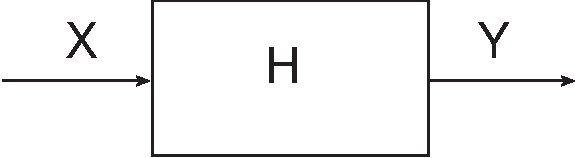
\includegraphics[width=0.5\textwidth]{ch-fir/ff-blackbox}}
\caption{Treat transfer function as a black box.
\label{fig:ff-blacbox}}
\end{figure}

We can treat the transfer function as a black box that does everything
that the filter needs to do. We only need to pay attention to the
input and output, as in figure~\ref{fig:ff-blacbox}.  This give us a
way to combine different filters, simply by composing block
diagrams. Consider two simple filters $H_1(z)$ and $H_2(z)$ connected
in series. $H_1(z)$ has input $X$ and output $W$, and $H_2(z)$ takes
$H_1(z)$'s output as its input and outputs $Y$. Starting from the
output of this system, this can be written
\begin{equation}
Y = H_2(z)W = H_2(z)[H_1(z)X]
  = \underbrace{[H_2(z)H_1(z)]}_{\text{combined transfer function}} X
\end{equation}

This suggests that the combined transfer function is
$H_2(z)H_1(z)$. In fact, we can interchange the order
\begin{equation}
H_2(z)H_1(z) = H_1(z)H_2(z)
\end{equation}
Because the transfer function is a polynomial, this gives us a way to
represent digital filtering as just multiplication by a polynomial
(and the product of two polynomials is just another polynomial).

\problemset{
\subsubsection{Self-Test Exercises}
\label{sc:ste-oper}

See~\ref{sc:ch3ex} \#\ref{it:ch3ex3}--\ref{it:ch3ex5} for answers.

\begin{enumerate}
\item Write equation~(\ref{eq:ff-manyk}) for $k=0, 1, 2, 3$, then
  write the transfer function for each.
\item Given the signal $x(t) = \sin t$ and the derivative operator
  $D=\derivin{}{t}$, what is $Dx(t)$?
\item When
  \begin{align*}
    H_1(z) &= b_0 + b_1z^{-1}\\
    H_2(z) &= b'_0 + b'_1z^{-1}
  \end{align*}
  and $b_0$, $b_1$, $b'_0$, and $b'_1$ are constants, show that
  $H_2(z)H_1(z) =
  H_1(z)H_2(z)$.
\end{enumerate}}

\subsection{The z-plane}

\index{z@$z$!complex plane}
We just used $z$ as a delay operator without much comment as to why we
picked it. In mathematics, the same symbol is used for the complex plane (also called the z-plane).  The
operator $z=e^{j\hat{\omega}}$ is a complex variable in the
z-plane. For any value of $\hat{\omega}$, it lies on a circle of radius one,
at an angle of $\hat{\omega}$ relative to the positive real axis --- it is
the polar representation of a complex number with a magnitude of one. As $\hat{\omega}$ varies from
zero to $2\pi$ (or $-\pi$ to $+\pi$, if you prefer not to consider
$\hat{\omega} > \hat{\omega}_\mathit{Nyquist}$), its path is the unit circle in
the z-plane. Since the Nyquist frequency
$\hat{\omega}_\mathit{Nyquist}=\pi$, we are only interested in the top of half
of the circle running from $\hat{\omega}=0$ to $\hat{\omega}=\pi$.

Using the complex plane makes filters easier to analyze (just like phasors!). To understand why, we will need to develop the relationship between the frequency response of a filter and the complex plane. Let's examine the defining equation of a simple digital filter with
one time delay:
\begin{equation}
y[n] = x[n]-b_1x[n-1]
\end{equation}
Just for convenience, we have used subtraction instead of summation
(or, equivalently you can think of using a negative weight on the
delayed signal). Using the delay operator $z$ and the transfer
function $H(z)$, this becomes:
\begin{equation}
Y = [1-b_1z^{-1}]X = H(z)X
\end{equation}
Obviously,
\begin{equation}
H(z) = 1-b_1z^{-1} = (1-b_1z^{-1}) \frac{z}{z} = \frac{z-b_1}{z}
\end{equation}

For our purposes, we shall restrict ourselves to considering $z$ to be
on the unit circle ($z=e^{j\hat{\omega}}$). The magnitude of $H(z)$ is
the same as the magnitude of $\mathcal{H}(\hat{\omega})$, so the
magnitude of the frequency response is
\begin{equation}
|\mathcal{H}(\hat{\omega})| = |H(z)|_{z=e^{j\hat{\omega}}}
       = \frac{|z-b_1|_{z=e^{j\hat{\omega}}}}{|z|_{z=e^{j\hat{\omega}}}}
       = |z-b_1|_{z=e^{j\hat{\omega}}}
\label{eq:ff-simplez}
\end{equation}
You can see that
although $z=0$ makes the denominator of $H(z)$ zero, we're not
considering that case --- we've already said that we're on the unit
circle: that $|z|=1$.  The value that makes the denominator of
$H(z)$ zero is called a \emph{pole}, which we will talk
about in a subsequent chapter.

Equation~(\ref{eq:ff-simplez}) tells us that the magnitude of the
transfer function is the distance between $z$ and $b_1$ in the complex
plane.  Since $z$ is a vector from the origin to the unit circle and
$b_1$ is a constant, which can be any number here,
$|\mathcal{H}(\hat{\omega})|$ is equal to the length of the vector
from $b_1$ to the unit circle where $z$ points. As this length becomes
shorter, $|\mathcal{H}(\hat{\omega})|$ becomes smaller. We can see
that is the case when $z$ nears $b_1$.

The other thing that equation~(\ref{eq:ff-simplez}) tells us is that
when $z=b_1$, $\mathcal{H}(\hat{\omega})=0$, so $b_1$ is a \emph{root}
of $\mathcal{H}(\hat{\omega})$ --- also called a \emph{zero} --- which
makes the magnitude of the frequency response reach its
minimum.
\index{zero}
\index{frequency response!zero}
Obviously, when the zero ($b_1$) is near $\hat{\omega}=0$ $(z=1)$,
this results in a high pass filter because it doesn't pass frequencies
near zero (low frequencies). Similarly, when the zero ($b_1$) is near
$\hat{\omega}=\pi$ $(z=-1)$ we obtain a low pass filter: high frequency
components are filtered out. In this way, we can graph the zeros of a filter in the z-plane to better understand its behavior. 

\paragraph*{Example 3:}

Consider the general two-time-step delay feedforward filter,
\begin{equation*}
y[n] = x[n] + b_1 x[n-1] + b_2 x[n-2]
\end{equation*}
where $b_1$ and $b_2$ are real constants. Let's analyze its
behavior. The transfer function is
\begin{align*}
H(z) &= 1 + b_1 z^{-1} + b_2 z^{-2} \\
     &= (1 + b_1 z^{-1} + b_2 z^{-2}) \frac{z^2}{z^2} \\
     &= \frac{z^2 + b_1 z + b_2}{z^2}
\end{align*}

The magnitude response is
\begin{equation}
|H(z)| = \frac{|z^2 + b_1 z + b_2|}{|z^2|} \label{eq:twostep-ex}
\end{equation}
It has two poles at zero; however, as we already know, $|z^2|=1$, so
they don't affect the magnitude response. So $|H(z)|$ becomes:
\begin{equation}
|H(z)|=|z^2 + b_1 z + b_2| \label{eq:twostep-ex-magresp}
\end{equation}
The zeros of this magnitude response are merely the roots of a
polynomial of order two,
\index{polynomial!order two!roots of}
\index{quadratic equation!roots of}
\begin{equation}
z_{1,2} = \frac{-b_1 \pm \sqrt{b_1^2 - 4 b_2}}{2}
\label{eq:ff-z0s}
\end{equation}

For real $b_k$, the possible types of zeros are:
\begin{itemize}
\item When $b_1^2 > 4b_2$, there are two real zeros.
\item When $b_1^2 = 4b_2$, there are repeated zeros at $-b_1$.
\item When $b_1^2 < 4b_2$, there are two complex conjugate zeros
\end{itemize}
Let's call the two solutions of equation~(\ref{eq:ff-z0s}) $z_1$ and
$z_2$.  Since these are the roots of the magnitude response, we can
factor the polynomial in~(\ref{eq:twostep-ex-magresp}) that describes
the magnitude response as:
\begin{equation}
|H(z)| = |(z - z_1)(z - z_2)| \label{eq:twostep-factored}
\end{equation}

\begin{figure}[t]
\centerline{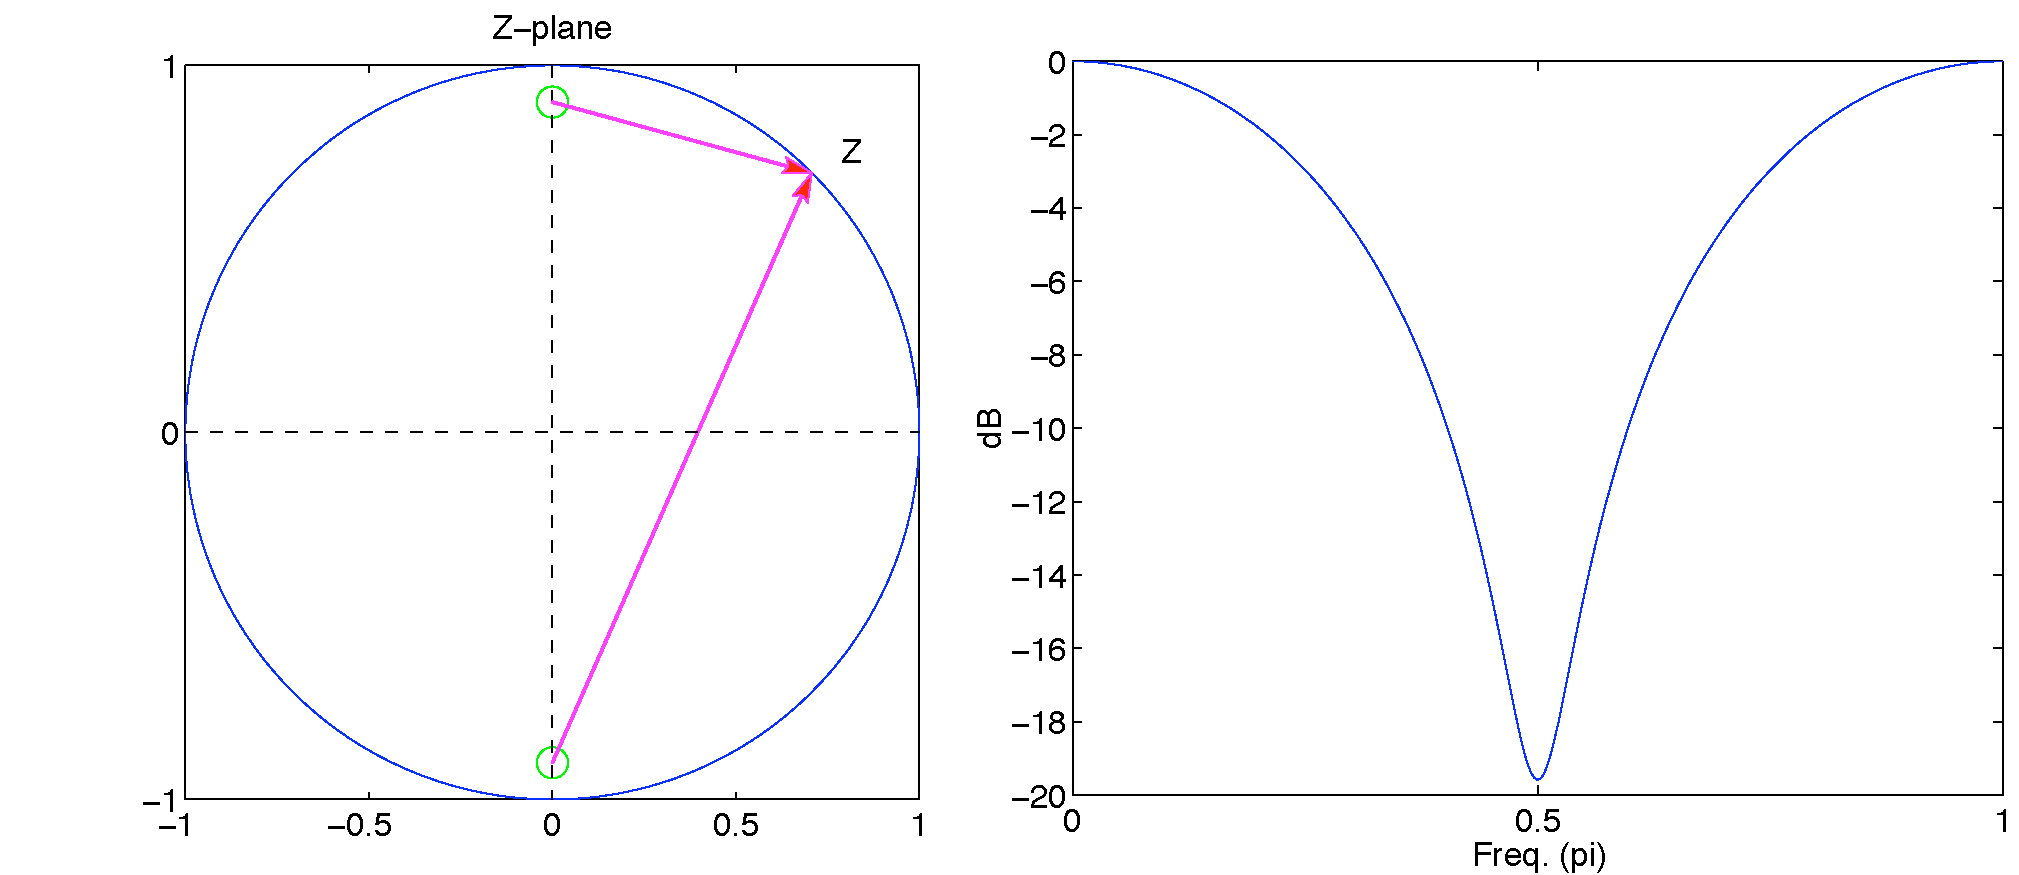
\includegraphics[width=6in]{ch-fir/ffexp_2tdelay_czh90_r0-9}}
\caption[Two zero filter $r=0.9$, $\hat{\omega}_0=\pm\pi/2$.]{Two zero feedforward filter with $r=0.9$, $\hat{\omega}_0=\pm\pi/2$ and magnitude of frequency response.
\label{fig:ff-exp2zs90}}
\end{figure}

\begin{figure}[t]
\centerline{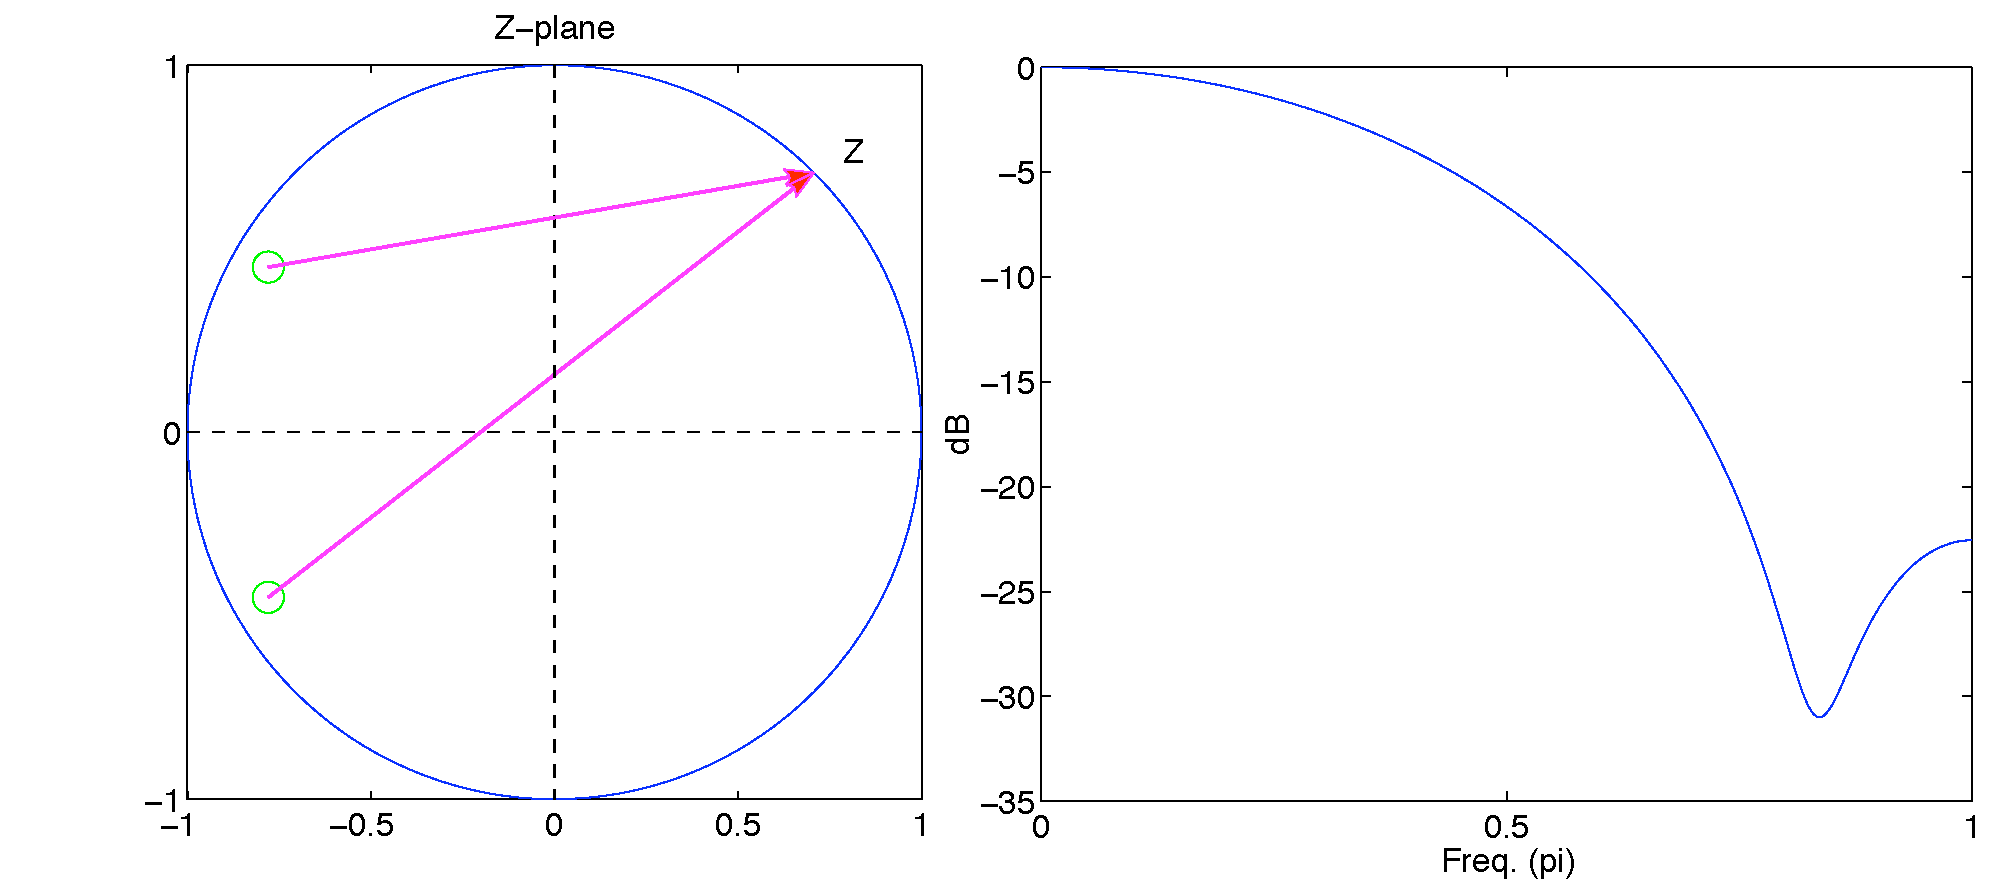
\includegraphics[width=6in]{ch-fir/ffexp_2tdelay_czh150_r0-9}}
\caption[Two zero filter $r=0.9$, $\hat{\omega}_0=\pm5\pi/6$.]{Two zero feedforward filter. $r=0.9$, $\hat{\omega}_0=\pm5\pi/6$ and magnitude of frequency response.
\label{fig:ff-exp2zs150}}
\end{figure}

%\begin{figure}
%\centerline{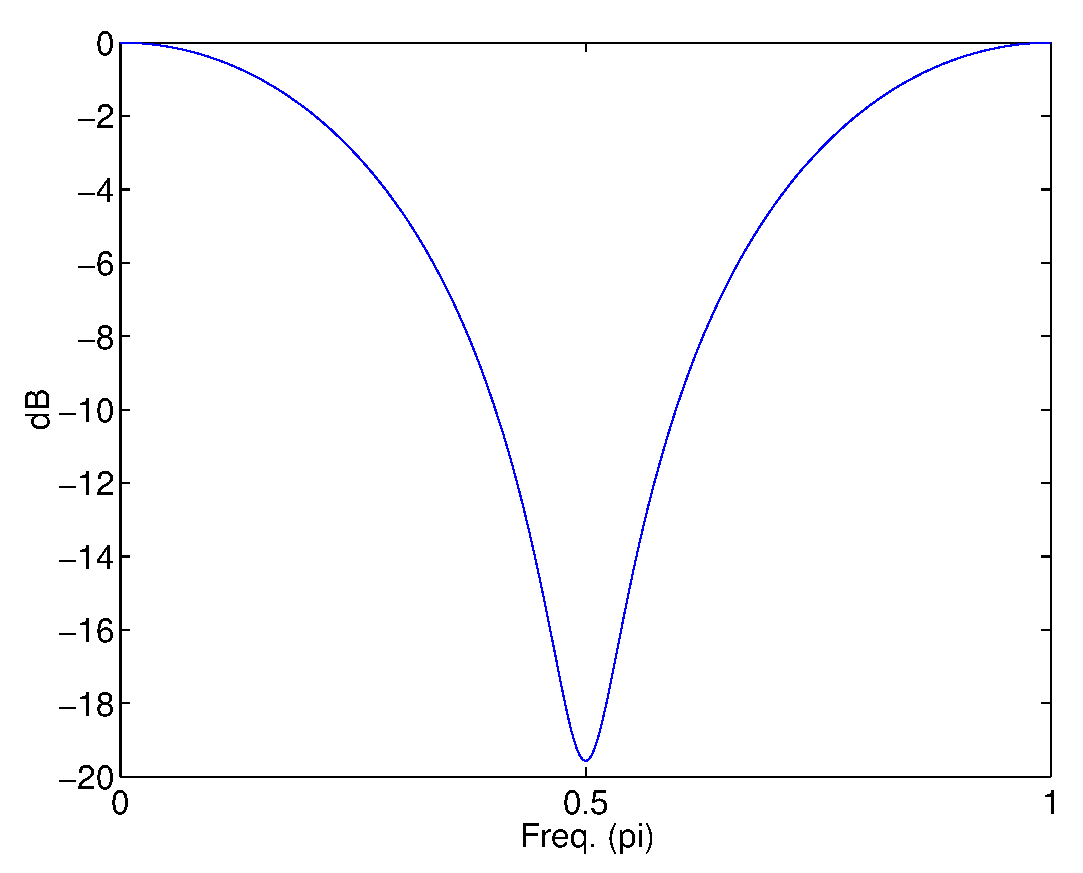
\includegraphics[height=3.5in]{ch-fir/ffexp_2tdelay_h90_r0-9}}
%\caption{Magnitude of frequency response for the filter in
%figure~\protect\ref{fig:ff-exp2zs90}.
%\label{fig:ff-exp2zh90}}
%\end{figure}
%
%\begin{figure}
%\centerline{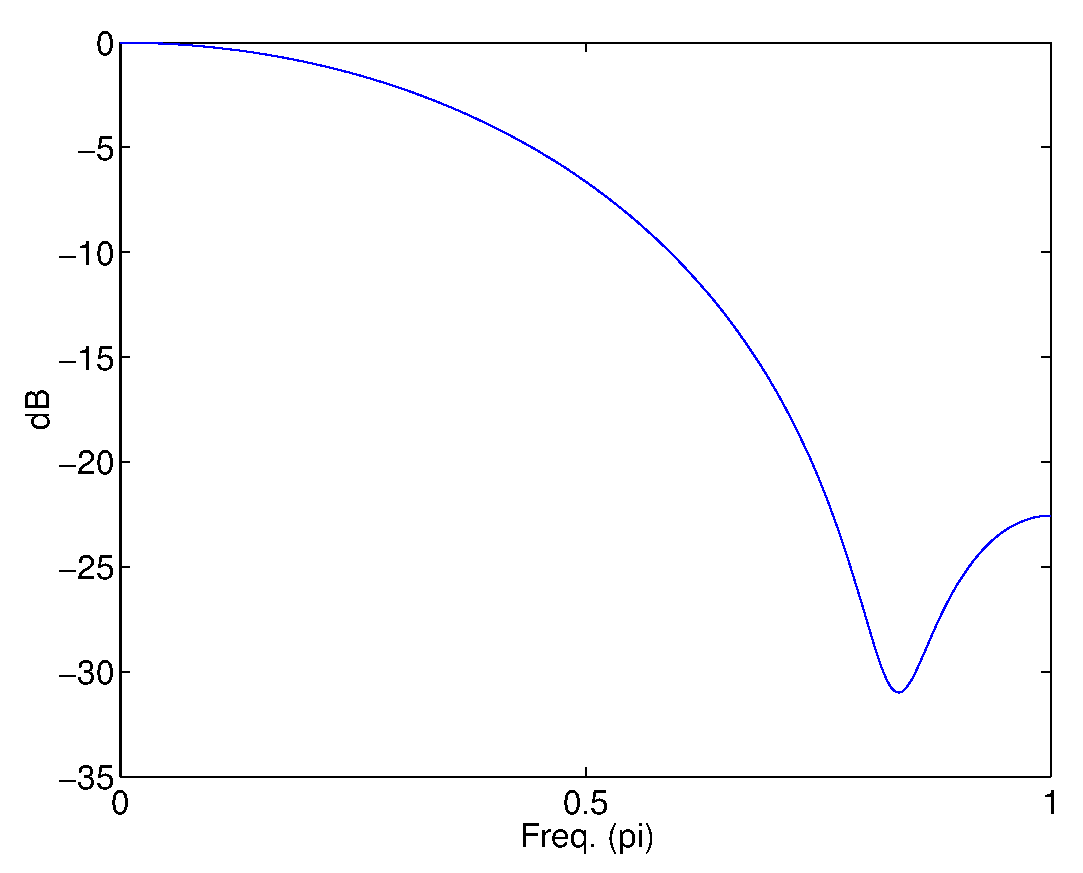
\includegraphics[height=3.5in]{ch-fir/ffexp_2tdelay_h150_r0-9}}
%\caption{Magnitude of frequency response for the filter in
%figure~\protect\ref{fig:ff-exp2zs150}.
%\label{fig:ff-exp2zh150}}
%\end{figure}

We can write the zeros in polar form, for convenience of
visualization, as
\begin{equation}
z_{i}=r_i e^{j \hat{\omega}_{0_i}}, \quad i=1,2
\end{equation}
where $r_i>0$ are the radii where the zeros are located, and
$\hat{\omega}_{0_i}$ their angles.  Depending on the angles
$\hat{\omega}_{0_i}$, the zeros can be either real or complex. For
example, when $\hat{\omega}_{0_i}=0$, the zero lies on the z-plane's
real axis, and when $\hat{\omega}_{0_i}=\pi/2$, it is on the imaginary
axis. Actually, when a filter's coefficients are real, if one of the
zeros is a complex number, the other one will be its conjugate mate
(if one of them is real, the other will be real, too).  So, in the
case where one zero is imaginary at $\hat{\omega}_{0_i}=\pi/2$, the
other zero's angle would be $\hat{\omega}_0=-\pi/2$. So, for this
filter and real coefficients, the pair of complex zeros can be written
as
\begin{equation}
z_{1,2}=r e^{\pm j \hat{\omega}_0}
\label{eq:ff-zero}
\end{equation}

Figures~\ref{fig:ff-exp2zs90} and~\ref{fig:ff-exp2zs150} show two
different sets of zero locations. The magnitude responses for
those two sets of zeros are also presented.

\subsection{Phase Response}

\index{filter!phase response|(emph}
So far we have been talking about the magnitude response of
$\mathcal{H}(\hat{\omega})$.  In the last topic of this chapter, let's
talk about is its phase response. We already know that
$\mathcal{H}(\hat{\omega})$ can be expressed in polar form, with its
magnitude and angle
\begin{equation}
\mathcal{H}(\hat{\omega})=|\mathcal{H}(\hat{\omega})|e^{j \theta(\hat{\omega})}
\end{equation}
$|\mathcal{H}(\hat{\omega})|$ is the magnitude response and
$\theta(\hat{\omega})$ is the phase response. The phase response can
be computed as
\begin{equation}
\theta(\hat{\omega}) = \angle\mathcal{H}(\hat{\omega})
 = \arctan\left(\frac{\Imag[\mathcal{H}(\hat{\omega})]}{\Real[\mathcal{H}(\hat{\omega})]}\right)
\label{eq:compute-phase-resp}
\end{equation}

When the input signal is a phasor, $x[n]=e^{jn\hat{\omega}}$, the
filter's output is
\begin{equation}
y[n] = \underbrace{|\mathcal{H}(\hat{\omega})|e^{j
    \theta(\hat{\omega})}}_{\mathcal{H}(\hat{\omega})} e^{jn\hat{\omega}}
= \underbrace{|\mathcal{H}(\hat{\omega})|}_{\text{change in magnitude}}
  \underbrace{e^{j(n\hat{\omega} +
      \theta(\hat{\omega}))}}_{\text{phase shift}}
\end{equation}
So, what a filter does to a phasor (one frequency of the input) is to
change the input's magnitude at that frequency by multiplying by
$|\mathcal{H}(\hat{\omega})|$ and shift its phase (which is the same
thing as delaying it) by the phase response $\theta(\hat{\omega})$.
\index{filter!phase response|)}

\paragraph*{Example 4:}

Let's examine the previous example (from the discussion of the z-plane):
\begin{equation*}
y[n] = x[n] + b_1x[n-1] + b_2x[n-2]
\end{equation*}
Its transfer function is
\begin{equation*}
H(z)=1 + b_1z^{-1} + b_2z^{-2} 
\end{equation*}
with the values $b_1=0$ and $b_2=1$. The frequency response can be separated into the magnitude and phase response according to,
\begin{align}
\mathcal{H}(\hat{\omega}) &= 1 + b_1e^{-j\hat{\omega}} + b_2e^{-2j\hat{\omega}}
\label{eq:ff-2zthosimple} \\
&= 1 + e^{-2j\hat{\omega}}  && (\text{substitute for $b_1, b_2$}) \notag\\
&= e^{-j\hat{\omega}} (e^{j\hat{\omega}}  + e^{-j\hat{\omega}})  &&
 (\text{factor out $e^{-j\hat{\omega}} $}) \notag \\
&=\underbrace{e^{-j\hat{\omega}}}_{\stackrel{\text{phase}}{_\text{response}}} 
\underbrace{2\cos(\hat{\omega})}_{\stackrel{\text{magnitude}}{_\text{response}}}  &&
 (\text{use Euler's formula}) \label{eq:ex4final}
\end{align}
The magnitude of equation~(\ref{eq:ex4final}) is:
\begin{equation}
|\mathcal{H}(\hat{\omega})|=2|\cos(\hat{\omega})|
\label{eq:ff-z0ssimp}
\end{equation}
and the phase is 
\begin{align}
\theta(\hat{\omega})
              &= \left\{\begin{array}{rl}
                         -\hat{\omega} & 0 \leq \hat{\omega} < \pi/2\\
                         \pi-\hat{\omega} & \pi/2 < \hat{\omega} \leq \pi
                        \end{array}\right.
                        \label{eq:ff-z0phasesimp}
\end{align}
Notice there is a jump of $\pi=180^\circ$ when the $\cos\hat{\omega}$ goes from positive to negative at $\hat{\omega}=\pi/2$. 

In other words \emph{both} the magnitude and phase responses are
functions of $\hat{\omega}$ --- they change the input in a
frequency-dependent way. According to equation~(\ref{eq:ff-z0ssimp}), the
two zeros of the transfer function are at:
\begin{equation*}
\hat{\omega}= \pm\frac{\pi}{2}
\end{equation*}
which, in the z-plane, are a pair of complex zeros on the imaginary axis. Using polar
coordinates they are
\begin{equation}
z_{1,2} = e^{\pm j\pi/2}
\end{equation}
with $r=1$. 

We can illustrate the effect of this filter in a simple manner by
examining the response when the input is a phasor (a single frequency,
$x[n]=e^{jn\hat{\omega}}$):
\begin{equation}
  y[n]= \mathcal{H}(\hat{\omega})x[n] 
      = 2\cos\hat{\omega} e^{j(n-1)\hat{\omega}} \label{eq:ff-2zt}
\end{equation}
We can see that the effect of the filter on the input signal is to
delay it by one sampling interval (from the $(n-1)$ term in the
exponential) and to multiply it by $2\cos\hat{\omega}$. Notice that
the delay is independent of its frequency. When all the frequency
components of a signal are delayed by an equal amount, say the filter
has \emph{no phase distortion} or \emph{linear phase}. The magnitude response and phase response are
shown in figure~\ref{fig:ff-exp2zh90-r1}.

\begin{figure}
\centerline{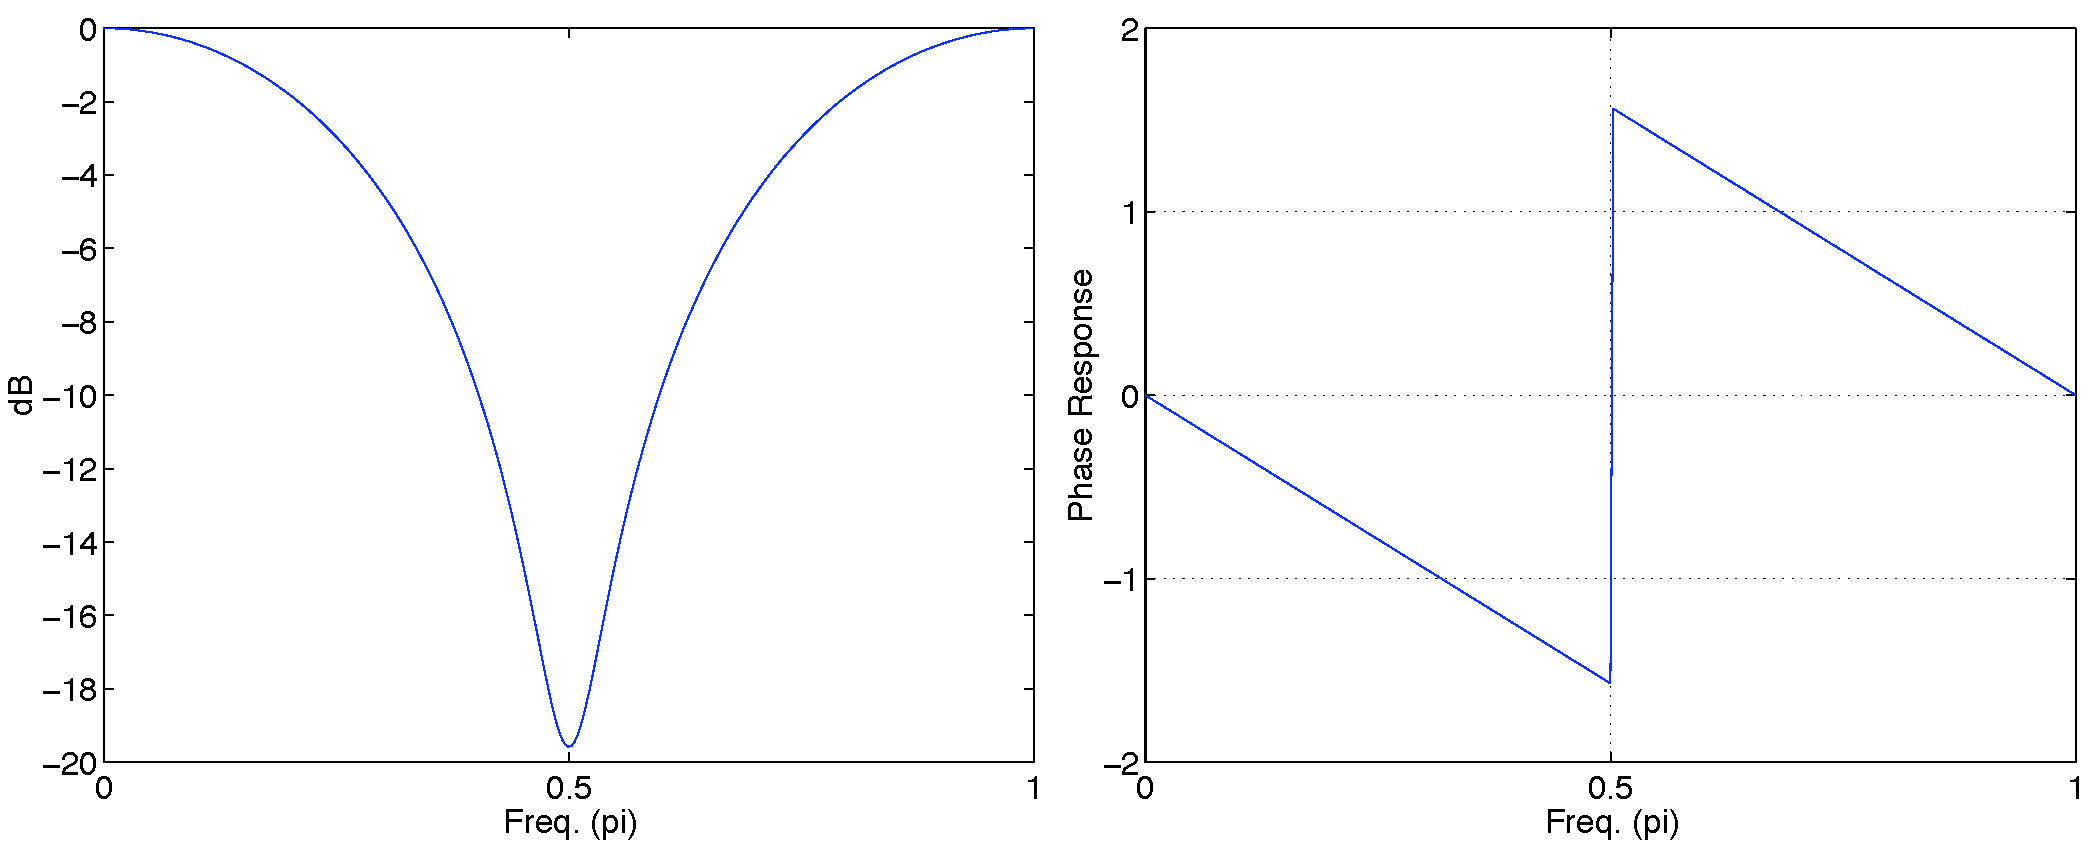
\includegraphics[width=6in]{ch-fir/ffexp_2tdelay_h90}}
\caption[Frequency response of two time delay feedforward
filter]{Magnitude and phase response of two time delay feedforward filter, with
$b_1=0, b_2=1$ in~(\protect\ref{eq:ff-2zt}).  Its zeros are at $e^{\pm
j\pi/2}$.
\label{fig:ff-exp2zh90-r1}}
\end{figure}

\paragraph*{Example 4: generic method [optional]}
There is also a more generic method to get the filter's phase response that will work for any value of $b_1$ and $b_2$, for which we need to access the frequency
response's real and imaginary parts. The frequency response
is
\begin{align}
\mathcal{H}(\hat{\omega}) &= 1 + b_1e^{-j\hat{\omega}} + b_2e^{-2j\hat{\omega}}
\label{eq:ff-2ztho} \\
     &= 1 + b_1(\cos\hat{\omega} - j\sin\hat{\omega})
        + b_2(\cos 2\hat{\omega} - j\sin 2\hat{\omega})
\notag \\
     &= \underbrace{(1 +b_1\cos\hat{\omega}+b_2\cos
       2\hat{\omega})}_{\Real[\mathcal{H}(\hat{\omega})]}
        \underbrace{-j(b_1\sin\hat{\omega}+b_2\sin
          2\hat{\omega})}_{j\Imag[\mathcal{H}(\hat{\omega})]}
\notag
\end{align}
where we have used Euler's formula to rewrite it so that we can
separate its real and imaginary components. We can obtain the
magnitude response from the square root of the sum of the square of
these components and the phase response using
equation~(\ref{eq:compute-phase-resp}).

When the magnitude response of a filter is plotted, the $y$ axis scale
is usually expressed in decibels (dB), a logarithmic scale. We can
take advantage of this to slightly simplify its
computation.  To do this, we note that the \emph{square} of the
magnitude response is the sum of the squares of the real and imaginary
components:
\begin{equation}
|\mathcal{H}(\hat{\omega})|^2=[1 +b_1\cos\hat{\omega}+b_2\cos 2\hat{\omega}]^2 +
              [b_1\sin\hat{\omega}+b_2\sin 2\hat{\omega}]^2
\label{eq:ff-exph1}
\end{equation}

\index{decibel}
A quantity is converted to dB by taking twenty times the logarithm
(base ten).  $|\mathcal{H}(\hat{\omega})|$ can be converted to dB as
\begin{align*}
|\mathcal{H}(\hat{\omega})|_{\mathit{dB}} &= 20\log_{10}|\mathcal{H}(\hat{\omega})|=10\log_{10}|\mathcal{H}(\hat{\omega})|^2
\\
           &= 10\log_{10}\left\{[1 +b_1\cos\hat{\omega}+b_2\cos 2\hat{\omega}]^2 +
               [b_1\sin\hat{\omega}+b_2\sin 2\hat{\omega}]^2\right\}
\end{align*}
Which is a trivial matter to compute for any value of $\hat{\omega}$ (on a
computer) for plotting purposes.  The phase response is
\begin{equation}
\theta(\hat{\omega})=\arctan\left[\frac{-(b_1\sin\hat{\omega}+b_2\sin 2\hat{\omega})}
                            {1 +b_1\cos\hat{\omega}+b_2\cos 2\hat{\omega}}\right]
\label{eq:ff-expph1}
\end{equation}

Consider the special case used in the previous example: $b_1=0$ and $b_2=1$ (a filter with a two-step
delay). Substituting these values into equations~(\ref{eq:ff-exph1})
and~(\ref{eq:ff-expph1}), the squared magnitude becomes
\begin{align*}
|\mathcal{H}(\hat{\omega})|^2 &= (1+\cos 2\hat{\omega})^2 + \sin^2 2\hat{\omega} \\
             &= 1+2\cos 2\hat{\omega}+\cos^2 2\hat{\omega}+\sin^2 2\hat{\omega} \\
             &= 1+2\cos 2\hat{\omega} + 1 \\
             &= 2(1+\cos 2\hat{\omega}) \\
             &= 2(1+2\cos^2 \hat{\omega}-1) \\
             &= 4\cos^2 \hat{\omega}
\end{align*}
Where the next to last step made use of the double-angle identity,
$\cos 2\theta = 2\cos^2 \theta - 1$.  The square root of this is
\begin{equation*}
|\mathcal{H}(\hat{\omega})|=2|\cos \hat{\omega}|
\end{equation*}
Which is exactly what we calculated in equation (\ref{eq:ff-z0ssimp})!

With the substitution, the phase response becomes
\begin{equation}
\theta(\hat{\omega})=\arctan\left(\frac{-\sin 2\hat{\omega}}{1+\cos 2\hat{\omega}}\right)
\label{eq:ff-expph2}
\end{equation}
If we remember the double-angle formulae,
\index{trigonometry!double-angle formulae}
\begin{align*}
\sin 2\hat{\omega} &= \frac{2\tan\hat{\omega}}{1+\tan^2\hat{\omega}} \\
\cos 2\hat{\omega} &= \frac{1-\tan^2\hat{\omega}}{1+\tan^2\hat{\omega}}
\end{align*}
and substitute them into equation~(\ref{eq:ff-expph2}), we get
\begin{align*}
\theta(\hat{\omega})&= \arctan\left(\frac{-2\tan\hat{\omega}}{2}\right) \\
              &= \arctan(-\tan\hat{\omega})\\
              &= \left\{\begin{array}{rl}
                         -\hat{\omega} & 0 \leq \hat{\omega} < \pi/2 \\
                         \pi-\hat{\omega} & \pi/2 < \hat{\omega} \leq \pi
                        \end{array}\right.
\end{align*}
Which is what we calculated in equation (\ref{eq:ff-z0phasesimp}). 

The final result for the transfer function, written in
polar form, is:
\begin{equation}
\mathcal{H}(\hat{\omega}) = |\mathcal{H}(\hat{\omega})|e^{j\theta(\hat{\omega})} = 
e^{-j\hat{\omega}}2\cos\hat{\omega} 
\label{eq:ff-2zth}
\end{equation}


\problemset{
\subsubsection{Self-Test Exercises}

See~\ref{sc:ch3ex} \#\ref{it:ch3ex6}--\ref{it:ch3ex7} for answers.

\begin{enumerate}
\item Prove $|z^2|=1$ in
  equation~(\ref{eq:twostep-ex}).
\item Starting with the factored magnitude response in
  equation~(\ref{eq:twostep-factored}), derive expressions for $b_1$
  and $b_2$ in terms of $z_1$ and $z_2$.
\end{enumerate}}

\subsection{Implementing Digital Filters}

\index{digital filtering!pseudocode|(}
Implementing feedforward digital filters is really quite
straightforward. Let's first look at how we would implement the two
time delay feedforward filter $y[n]=x[n]+b_1x[n-1]+b_2x[n-2]$, when
$b_1=0, b_2=1$, using pseudocode.  I'll present segments of a script
to do the computation and plot some results with my comments on it
interspersed.

\begin{algorithm}
\caption{Generate two sinusoids.\label{alg:gensine}}
\begin{algorithmic}
\STATE $F_s=100$, $N=100$, $T_s=1/F_s$
\STATE $f_1=5$ and $f_2=25$
\FOR{$n=0, 1, 2, \ldots N-1$}
   \STATE $x[n] = \sin(2\pi f_1 n T_s)+\sin(2\pi f_2 n T_s)$
\ENDFOR
\end{algorithmic}
\end{algorithm}

%\begin{small}
%\begin{verbatim}
%% exp_ff_filter.m				
%% feedforward filter : y_t = x_t + b1x_t + b2x_t
%% when a1=0, a2=1;
%
%clf;
%clear
%
%% --- Generate an input signal --- 
%Fs=100;                 % Sampling frequency Fs, samples/second
%N=100;                  % make N samples
%Ts = 1/Fs;              % time interval, seconds/sample
%t = (1:N)*Ts;           % discrete time axis (sample times, in seconds)
%f1 = 5;                 % input signal's frequency
%f2 = 25;
%b1 = 0;                 % filter coefficients
%b2 = 1;
%x=sin(2*pi*t*f1)+sin(2*pi*t*f2);      % input signal 
%\end{verbatim}
%\end{small}

In algorithm~\ref{alg:gensine}, we've generated a discrete signal $x$ containing sine wave values at all the time points at which
the sampling should occur (100 samples at 100Hz = 1 second). The
signal has two frequency components: one at 5Hz and one at 25Hz (both
well below the Nyquist frequency).

\begin{algorithm}
\caption{Filtering.\label{alg:filtering}}
\begin{algorithmic}
\STATE $b_1=0$ and $b_2=1$
\STATE $y[0]=0$ and $y[1]=0$
\FOR{$n=2, 3, 4  \ldots N-1$}
   \STATE $y[n] = x[n]+b_1x[n-1]+b_2x[n-2]$
\ENDFOR
\end{algorithmic}
\end{algorithm}
%\begin{small}
%\begin{verbatim}
%% --- Filtering ---
%y = zeros(size(x));
%y(3:N) = x(3:N) + b1*x(2:N-1) + b2*x(1:N-2);
%y = real(y);
%\end{verbatim}
%\end{small}

In algorithm~\ref{alg:filtering}, we have the luxury of being able to
hold the entire input and output signal in arrays. Because there is a two time step delay, we
can't compute a value for $y[0]$ or  $y[1]$, so those are set to zero. 

%\begin{algorithm}
%\caption{Calculate spectra.\label{alg:spectra}}
%\begin{algorithmic}
%\STATE $X$=\verb|fft|($x$), take 512 point fast Fourier transform of $x$
%\STATE $Y$=\verb|fft|($y$), take 512 point fast Fourier transform of $y$
%\FOR{$k=0, 1, 2,  \dots 256$}
%   \STATE Plot abs($X[k]$) and abs($Y[k]$) at frequency $k\times F_s/512$
%\ENDFOR
%\end{algorithmic}
%\end{algorithm}

%\begin{small}c  x
%\begin{verbatim}
%% --- plot magnitude of the input and output signals' spectra ---
%spx=fft(x,512);         % original signal's fft
%spy=fft(y,512);
%fstep=(Fs/2)/256;       % frequency step
%f=(0:255)*fstep;        % frequency axis
%plot(f,abs(spx(1:256)'), 'g', f,abs(spy(1:256)'), 'm');
%                        %plot spx and spy in the same plot
%xlabel('Freq. (Hz)', 'Fontsize', 16);
%ylabel('Freq. Components', 'Fontsize', 16);
%set(gca, 'Fontsize', 16);
%input('Press key to continue')
%\end{verbatim}
%\end{small}

%TODO replace with intuition
After we filter the sum of sinusoids, we want to see what happened to the signal's frequency components. We will use the fast Fourier Transform to analyze the components. We'll talk about
the Fourier transform and FFT in section~\ref{sc:fourier-xform}.
Figure~\ref{fig:ff-expsin2_sp} shows the magnitude of each frequency in the generated and filtered sine waves. From the plot we can see that the high frequency wave is completely filtered out. And finally, we'll plot the input and output. They're shown in
figure~\ref{fig:ff-expsin2_sp} (right).

%\begin{small}
%\begin{verbatim}
%% --- Plot orignal and filtered signal ---
%plot(t, x, 'b', t, y, 'r' );
%xlabel('Time (sec)', 'FontSize', 16);
%ylabel('Time waveform', 'FontSize', 16);
%set(gca, 'FontSize', 16);
%\end{verbatim}
%\end{small}
%\index{MATLAB code!digital filtering|)}

How would one implement this in a language like C, C++, Java, etc?
Let's not worry about the plotting issue: that would certainly have to
be dealt with, but it would involve either getting a graphics library,
writing one's own, or using an external plotting package (ideally, one
targeted at scientific and engineering applications, rather than one
written for business).  For example, a fine alternative would be to 
vectorize all the array operations and use MATLAB.  We will
discuss the \verb|fft()| function in section~\ref{sc:fft}. The
only remaining issue is that of keeping the entire input and output
signal in memory.
\begin{figure}
\centerline{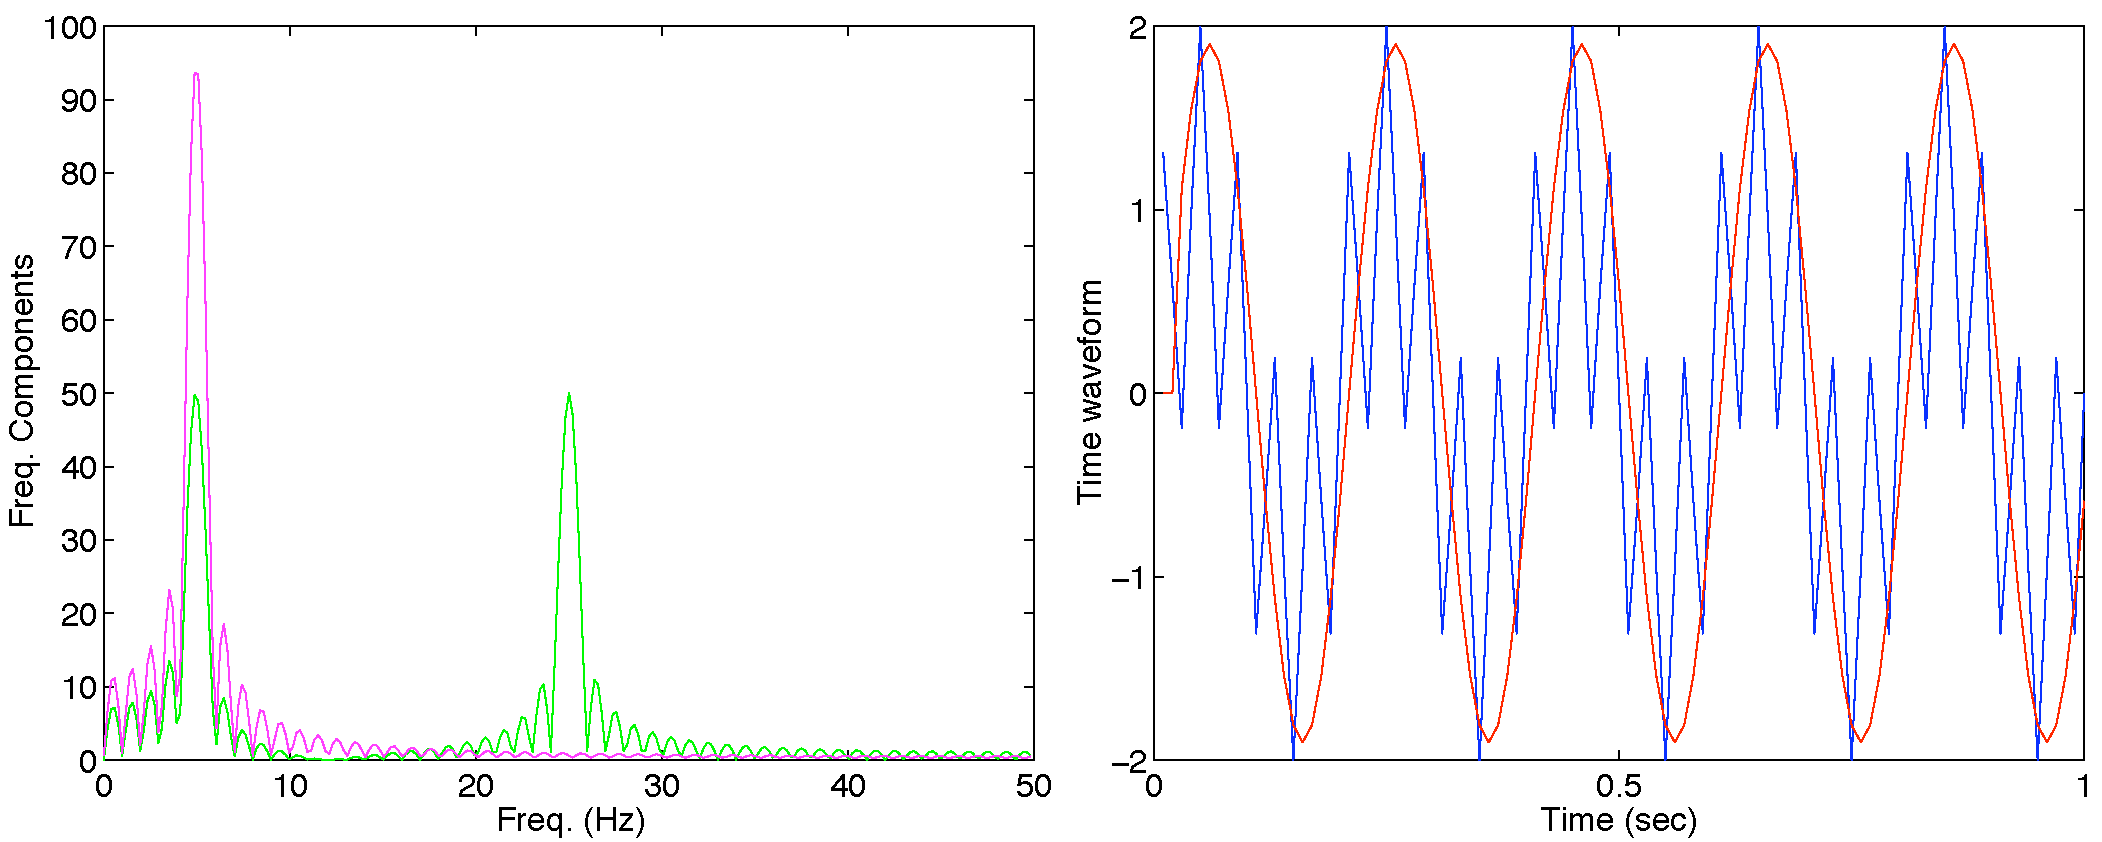
\includegraphics[width=6in]{ch-fir/sine2_ff2td_sp_wv}}
\caption[Two sinusoid spectrum]{The spectrum of a two frequency component sine wave and its filtered version,
using the feedforward filter $y[n]=x[n]+x[n-2]$, $f_1=5Hz$ and
$f_2=25Hz$. Zeros are at $z_0=0.99e^{\pm j\pi/2}$. The time waveforms are also shown.
\label{fig:ff-expsin2_sp}}
\end{figure}

%\begin{figure}
%\centerline{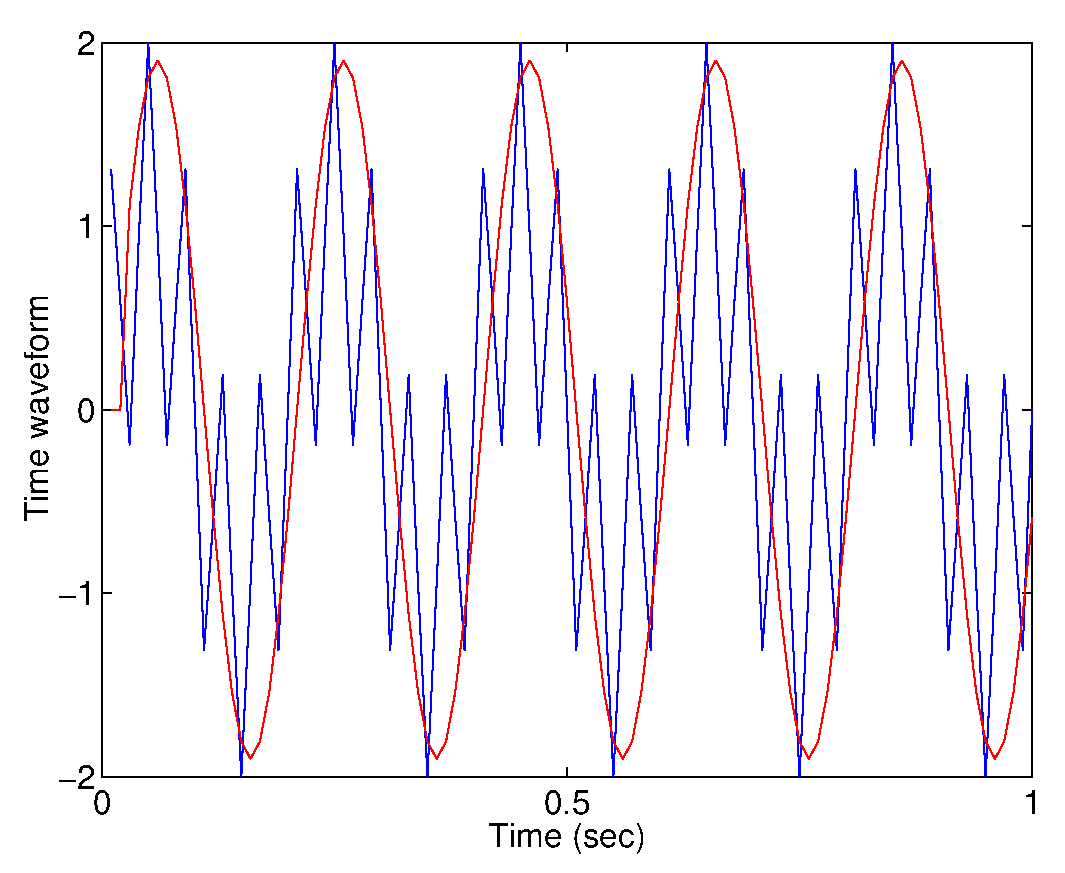
\includegraphics[width=4in]{ch-fir/sine2_ff2td}}
%\caption[Two frequency component sine wave and its filtered
%version]{Two frequency component sine wave and its filtered version,
%using the feedforward filter $y[n]=x[n]+x[n-2]$, $f_1=5Hz$ and
%$f_2=25Hz$. Zeros are at $z_0=0.99e^{\pm j\pi/2}$.
%\label{fig:ff-expsin2}}
%\end{figure}
In general, it is not possible to keep the entire input and output
signal in memory. In fact, many (if not most) digital signal
processing applications involve real-time processing, so the computer
system really needs to be viewed as just a stage in a processing
pipeline, with the input flowing in and the output flowing out (just
like the block diagrams used to illustrate filters).  We can therefore
only devote a relatively small amount of memory to hold the part of
the input and output needed for the current computation. If $n$
delayed samples of the input are needed to compute each output value,
we will need storage for $n+1$ input samples (the current one plus the
delayed samples). For a feedforward filter, there is no need to save
output values; they can be sent out as soon as they are computed.

What abstract data type (ADT) should hold the delayed inputs (answer
in~\ref{sc:ch3ex} \#\ref{it:ch3ex8})?  As each input sample comes in,
it displaces the oldest input sample from our buffer of $n+1$
values. For computer scientists, this is clearly a first-in-first-out (FIFO) ADT --- a \emph{queue}. A queue is very efficiently and simply implemented in an
array, especially when the queue size is fixed. Furthermore, you
can treat the array as though it were circular
using indexing modulo the queue size.

\section{Problems}

\begin{enumerate}
\item In Example~4, we used a large number of trigonometric identities
  to go from the filter's frequency response in~(\ref{eq:ff-2ztho}) to
  the results in~(\ref{eq:ff-2zth}) and~(\ref{eq:ff-2zt}) for the
  special case of $b_1=0$ and $b_2=1$. There is an easier way. First,
  substitute the values of $b_{1,2}$ into~(\ref{eq:ff-2ztho}), and then
  use the fact that we can always factor a real number into a product of
  complex conjugate numbers, i.e., $1 = e^{j\hat{\omega}}
  e^{-j\hat{\omega}}$. A little bit of algebra and Euler's formula
  should allow you to derive the results (\ref{eq:ff-2zth}) and
  (\ref{eq:ff-2zt}) of Example~4 much easier.
\item For the filter whose magnitude response is described
  in~(\ref{eq:twostep-factored}), plot the location of a pair of complex
  conjugate zeros at $r=0.8$ and $\hat{\omega}_0=\pm\pi/4$. Using MATLAB,
  compute and plot the filter's magnitude response. Submit your code
  with your figures.
\item In the self-test exercise on page~\pageref{sc:ste-oper}, two
  filters with transfer functions $H_1(z) = b_0 + b_1z^{-1}$ and
  $H_2(z) = b'_0 + b'_1z^{-1}$ were connected in series, and it was
  shown that they could be connected in either order to produce the same
  composite effect (the same overall transfer function). Redo this
  exercise using the defining equations for the two filters, i.e.,
  $y_1[n] = F_1(x[n])$ for the filter with transfer function $H_1(z)$
  and $y_2[n] = F_2(x[n])$ for the filter with transfer function
  $H_2(z)$. In other words, show that $F_2(F_1(x[n])) =
  F_1(F_2(x[n]))$.
\item Use MATLAB to plot the results of filtering the following
  signals with the filter: $y[n] = x[n] + x[n-1]$.  Submit your code
  with your results.
  \begin{enumerate}
  \item $x[n] = n$
  \item $x[n] = \sin(n\pi/100)$
  \item $\displaystyle
    x[n] = \left\{\begin{array}{ll}+1 & \quad n \bmod 5 \;\mathrm{even}\\
        -1 & \quad n \bmod 5 \;\mathrm{odd}\end{array}\right. $
  \end{enumerate}
\item Check the following factorization: $z^2 - z + 1 = (z -
  e^{j\pi/3}) (z - e^{-j\pi/3})$
\end{enumerate}

\section{Further Reading}

\begin{itemize}
\item James H McClellan, Ronald W. Schafer, and Mark A. Yoder, \textit{DSP
  First: A Multimedia Approach}, Prentice Hall, 1998, ch. 5 (\S
5.1--5.3), 6 (\S 6.1, 6.4--6.7).
\end{itemize}

% LocalWords:  MATLAB feedforward phasor response's


% -*-LaTeX-*-

% $Log: convolution.tex,v $
% Revision 1.6  2007/12/11 02:32:54  stiber
% Small edits for start of Winter 2008.
%
% Revision 1.5  2007/03/20 23:53:12  stiber
% Updated LaTeX.
%
% Revision 1.4  2007/03/20 01:25:56  stiber
% Modifications made to make this a standalone text.
%
% Revision 1.3  2006/03/27 23:36:42  stiber
% Fixed error in formula.
%
% Revision 1.2  2004/03/29 19:51:48  stiber
% Updated for Spring 2004 and new textbook (DSP First).
%
% Revision 1.1  2004/02/19 00:26:01  stiber
% Initial revision
%

\chapter{The Z-Transform and Convolution}
\label{ch:convolution}

Two signal processing tools --- the \emph{z transform} and
\emph{convolution} --- are introduced in this chapter.  These
operations play important roles in the analysis of discrete-time
signals (which is what we do in the computer). We shall see that they
are related --- the convolution of two time-domain signals (which is
what we do when we filter a signal) is equivalent to multiplication of
their corresponding z-transforms. This is one example of how these
representations can greatly simplify computation.

After studying this chapter, you should be able to understand what the
z-transform and convolution are, and how to implement them. You should
understand the differences between them and the other transforms:
Fourier series, Fourier transform, and discrete Fourier transform. You
will enrich your knowledge of filter transfer functions with its time
domain representation: its \emph{impulse response}.

\section{Domains}

Up to this point, we have covered the Fourier series representation of
a signal as a weighted sum of sinusoids. In effect, the Fourier series
\emph{transforms} a finite and periodic, continuous signal in the time
\emph{domain} into an infinite, discrete spectrum in the frequency
\emph{domain}.
\index{domains}
\index{time domain}
\index{frequency domain}
\index{domain!time}
\index{domain!frequency}
When we use the term \emph{domain}, we merely mean a particular way of
looking at a signal. In this case, we have two different ways of
thinking about our signals: as functions of time or as functions of
frequency. These are equivalent, in the sense that we can convert the
signal's representation back and forth between the two domains without
loss of information (neglecting matters such as roundoff error).

In future chapters, we will cover two other transforms:
\begin{description}
\item[Fourier transform] transforms an infinite, continuous signal in
the time domain into an infinite, continuous spectrum in the frequency
domain.

\item[Discrete Fourier transform] transforms a finite, discrete signal
in the time domain into a finite, discrete spectrum in the frequency
domain.
\end{description}

Here, however, we will learn about the
\emph{z-transform}, which converts an infinite, discrete signal in the
time domain into a finite, continuous spectrum in the frequency
domain. The z-transform fills the last combination among ``finite vs.
infinite; continuous vs. discrete''. Table~\ref{tb:zt-transforms}
summarizes all four transforms.  As you can see, continuous versus
discrete in the time domain transforms to infinite versus finite in
the frequency domain, while finite versus infinite in the time domain
transforms to discrete versus continuous in the frequency domain.

\begin{table}
\caption{Summary of frequency transforms.
\label{tb:zt-transforms}}
\begin{center}
\begin{tabular}{|l|l|l|} \hline
Transform & Time Domain & Frequency Domain\\ \hline\hline
Fourier Series & Finite, Continuous & Infinite, Discrete \\ 
Fourier Transform & Infinite, Continuous & Infinite, Continuous \\ 
Discrete Fourier Transform & Finite, Discrete & Finite, Discrete \\ 
Z-Transform & Infinite, Discrete & Finite, Continuous \\ \hline
\end{tabular}
\end{center}
\end{table}

\section{The z-transform}
The \emph{z-transform} of a discrete time signal $x[n]$, $n=0, \pm 1,
\pm 2, \ldots, \pm\infty$ is defined as the power series
\begin{equation}
X(z) \equiv \sum_{k=-\infty}^{\infty} x[k] z^{-k}
\label{eq:zt}
\end{equation}
where $z$ is a continuous complex variable. It transforms the time
domain, infinite, discrete sequence into its complex plane
representation $X(z)$. Since the z-transform is an infinite power
series, it exists only for those values of $z$ for which this series
converges. The \emph{region of convergence} (ROC) of $X(z)$ is the set
of all values of $z$ for which $X(z)$ has a finite value. We consider
the z-transform to be a transform between the time domain and the
frequency domain because we can substitute $z=e^{j\hat{\omega}}$ into
equation~(\ref{eq:zt}) to get the signal's (finite and continuous)
frequency content $\mathcal{X}(\hat{\omega})$ --- just as we
previously made the same substitution to derive a feedforward filter's
frequency response from its transfer function.

The relationship between $x[n]$ and $X(z)$ can be indicated
by the \emph{transform pair}
\begin{equation}
\underbrace{x[n]}_{\stackrel{\text{function of}}{_\text{sample \#}}}
   \stackrel{\mathbf{Z}}{\longleftrightarrow} 
   \underbrace{X(z)}_{\stackrel{\text{function of}}{_\text{complex $z$}}}
\end{equation}

\problemset{
\subsubsection{Self-Test Exercises}

See~\ref{sc:ch6ex} \#\ref{it:ch6ex1}--\ref{it:ch6ex2} for answers.

\begin{enumerate}
\item Determine the z-transform for the sequence
  $x[n]=\{1,2,5,7,0,1\}$, $n=0,1,2,3,4,5$

\item Determine the z-transform of the sequence
  $x[n]=\{1,2,5,7,0,1\}$, $n=-2,-1,0,1,2,3$
\end{enumerate}}

\subsection{Example: z-transform of an impulse}
\label{sc:zx-impulse}

\index{z-transform!of an impulse}
\index{unit impulse}
The \emph{unit impulse} or \emph{unit sample} signal is the $\delta$
function,
\begin{equation}
\delta[n] = \left\{\begin{array}{ll}
                        1 & n=0 \\
                        0 & n \neq 0
          \end{array}\right.
\end{equation}
It has value of zero for every sample except $n=0$, for which it has a
value of one. Substituting this signal into~(\ref{eq:zt}) to get its
z-transform, we have
\begin{align}
\Delta(z) &= \sum_{k=-\infty}^{\infty} \delta[k] z^{-k} \notag\\
     &= 1z^{-0}=1
\end{align}
that is 
\begin{equation}
\delta[n]\stackrel{\mathbf{Z}}{\longleftrightarrow} 1
\end{equation}

Since the frequency content of the signal is the magnitude of its
z-transform on the unit circle in the z-plane, 
\begin{equation}
|\mathcal{D}(\hat{\omega})|=|\Delta(e^{j\hat{\omega}})|=1
\label{eq:zt-delta}
\end{equation}
This tells us that the frequency content is the same for all
frequencies: an impulse has a \emph{flat spectrum}.

What about time shifted impulses,
\begin{align}
\delta[n-n_0] &= \left\{\begin{array}{ll}
                        1 & n=n_0 \\
                        0 & n \neq n_0
          \end{array}\right., \quad n_0>0 \\
\delta[n+n_0] &= \left\{\begin{array}{ll}
                        1 & n=-n_0 \\
                        0 & n \neq -n_0
          \end{array}\right., \quad n_0>0
\end{align}
In these cases the nonzero value is not at sample zero, but at samples
$n_0$ or $-n_0$.  We can compute the z-transform as before,
\begin{align}
\Delta(z) &= \sum_{k=-\infty}^{\infty} \delta[k-n_0] z^{-k} \notag\\
          &= 1z^{-n_0}=z^{-n_0}=\frac{1}{z^{n_0}}
\end{align}
for $\delta[n-n_0]$.  The z-transform for this shifted unit impulse
has one value, $z^{-n_0}$, for any $z \neq 0$.
\begin{equation}
\delta[n-n_0] \stackrel{\mathbf{Z}}{\longleftrightarrow} \frac{1}{z^{n_0}},
\quad n_0>0
\end{equation}

Its frequency content is also one, just like $\delta[n]$ (remember
that we compute the spectrum for values of $z$ on the unit circle),
\begin{equation}
|\mathcal{D}(\hat{\omega})|=|\Delta(e^{j\hat{\omega}})|=|e^{-jn_0\hat{\omega}}|=1
\end{equation}
This is not surprising at all, because it is, after all, just a
time-shifted version of $\delta[n]$. The signal $\delta[n+n_0]$ is
left as a self-test exercise.

\problemset{
\subsubsection{Self-Test Exercises}

See~\ref{sc:ch6ex} \#\ref{it:ch6ex3}--\ref{it:ch6ex4} for answers.

\begin{enumerate}
\item Sketch equation~(\ref{eq:zt-delta}).
\item Compute the z-transform and frequency content for the signal
  $\delta[n+n_0]$.
\end{enumerate}}

\subsection{Example: z-transform of exponential signal}
\label{sc:zx-exp}

\index{z-transform!of an exponential}
An exponential signal is defined as 
\begin{equation}
x[n] = \left\{\begin{array}{ll}
                        \alpha^n & \quad  n \ge 0 \\
                        0        & \quad n < 0
          \end{array}\right.
\label{eq:zt-expof}
\end{equation}
where $\alpha$ can be any real or complex value less than one. The
signal consists of an infinite number of samples. The z-transform of
this signal is
\begin{align}
X(z) &= \sum_{k=-\infty}^{\infty} x[k] z^{-k} \notag\\
     &= \sum_{k=0}^{\infty}\alpha^k  z^{-k} \notag\\
     &= \sum_{k=0}^{\infty}(\alpha z^{-1})^k
\label{eq:exp-zt}
\end{align}

This is an infinite \emph{geometric series}: a sum in which each
successive term is the previous term times some (unchanging)
expression (i.e., the ratio of successive terms is constant).
\index{geometric series} The ratio of two successive terms in a
geometric series like \index{geometric series!common ratio}
equation~(\ref{eq:exp-zt}) is called its \emph{common ratio}, which in
this case is $\alpha z^{-1}$. We can show this by rewriting
equation~(\ref{eq:exp-zt}) as $X(z) = 1 + \alpha z^{-1} + \alpha^{2}
z^{-2} + \cdots$. Rewriting the \spscript{$i+1$}{st} element of this
series as a recurrence relation (in terms of the \spscript{$i$}{th}),
\index{recurrence relation}
we get $X(z)_{i+1} = X(z)_i \alpha z^{-1}$, which shows the common ratio.
  
If we have a geometric series in which successive terms $b_i$ and
$b_{i+1}$ have the common ratio $r$ (i.e., $b_{i+1}/b_i = r$), then
any term in the series can be expressed in terms of the first term as
\index{geometric series!as function of first term}
\begin{equation*}
b_i = b_0 r^i
\end{equation*}
So, a geometric series can be expressed as a sum of these, $b_0 + b_0r
+ b_0r^2 + \cdots$. We can factor out the zeroth term, leaving us with
the task of simplifying $1 + r + r^2 + \cdots$. Multiplying this sum
by $(1-r)/(1-r)$, we obtain
\begin{align}
(1 + r + r^2 + \cdots)\frac{1-r}{1-r}
  & = \frac{1 + r + \cdots - r - r^2 - \cdots}{1-r} \notag\\
  & = \frac{1-r^N}{1-r}
\end{align}

In this case, $|r|<1$ so $r^N \rightarrow 0$ as $N \rightarrow \infty$:
\begin{equation}
1+r+r^2+r^3+\ldots = \frac{1}{1-r}, \quad\text{if } |r|<1
\end{equation}
Consequently, for $|r|=|\alpha z^{-1}|<1$ or $|z|>|\alpha|$,
$X(z)$ converges to
\begin{equation}
X(z)=\frac{1}{1-\alpha z^{-1}}, \quad |z|>|\alpha|
\label{eq:zt-expoF}
\end{equation}

In the z-plane, $|z|>|\alpha|$ refers to any $z$ that is outside of
the radius $|\alpha|$ circle. We see that in this case, the
z-transform provides a compact alternative representation of the
signal $x[n]$.

Let's check out some special cases:

\begin{figure}
\centerline{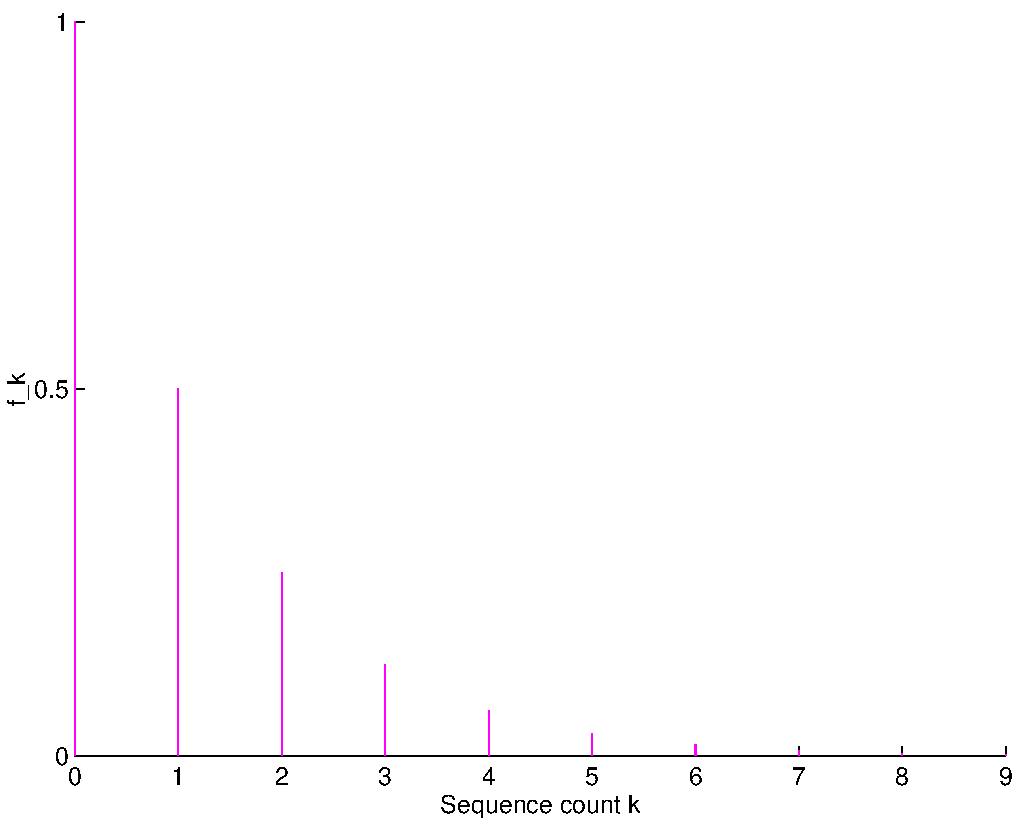
\includegraphics[width=3.5in]{ch-conv/zt_expo_rf}}
\caption{The exponential signal $x[n]=(1/2)^n, n=0,1,2,\ldots$.
\label{fig:zt-expo-r0.5f}}
\end{figure}

\paragraph*{When $\alpha$ is a real number, say $\alpha=1/2$:}
The discrete signal in this case is 
\begin{equation}
x[n] = \left\{\begin{array}{ll}
                        \left(\frac{1}{2}\right)^n & \quad  n \ge 0 \\
                        0             & \quad n < 0
          \end{array}\right.
\end{equation}
or
\begin{equation}
x[n] = \left\{1, \frac{1}{2}, \left(\frac{1}{2}\right)^2,
        \left(\frac{1}{2}\right)^3, \ldots, \right\}
\end{equation}
Figure~\ref{fig:zt-expo-r0.5f} shows the graph of the signal $x[n]$.

Replacing $\alpha$ with $1/2$ in~(\ref{eq:zt-expoF}), its
z-transform is expressed as
\begin{equation}
X(z)=\frac{1}{1-\frac{1}{2}z^{-1}}, \quad |z|>\frac{1}{2}
\end{equation}

As you should be familiar with now, the frequency content of this
signal is the magnitude of its z-transform on the unit circle
$z=e^{j\hat{\omega}}$ in the z-plane, which is
\begin{equation}
|\mathcal{X}(\hat{\omega})|=|X(e^{j\hat{\omega}})|
           =\left|\frac{1}{1-\frac{1}{2}e^{-j\hat{\omega}}}\right|
\end{equation}

\begin{figure}
\centerline{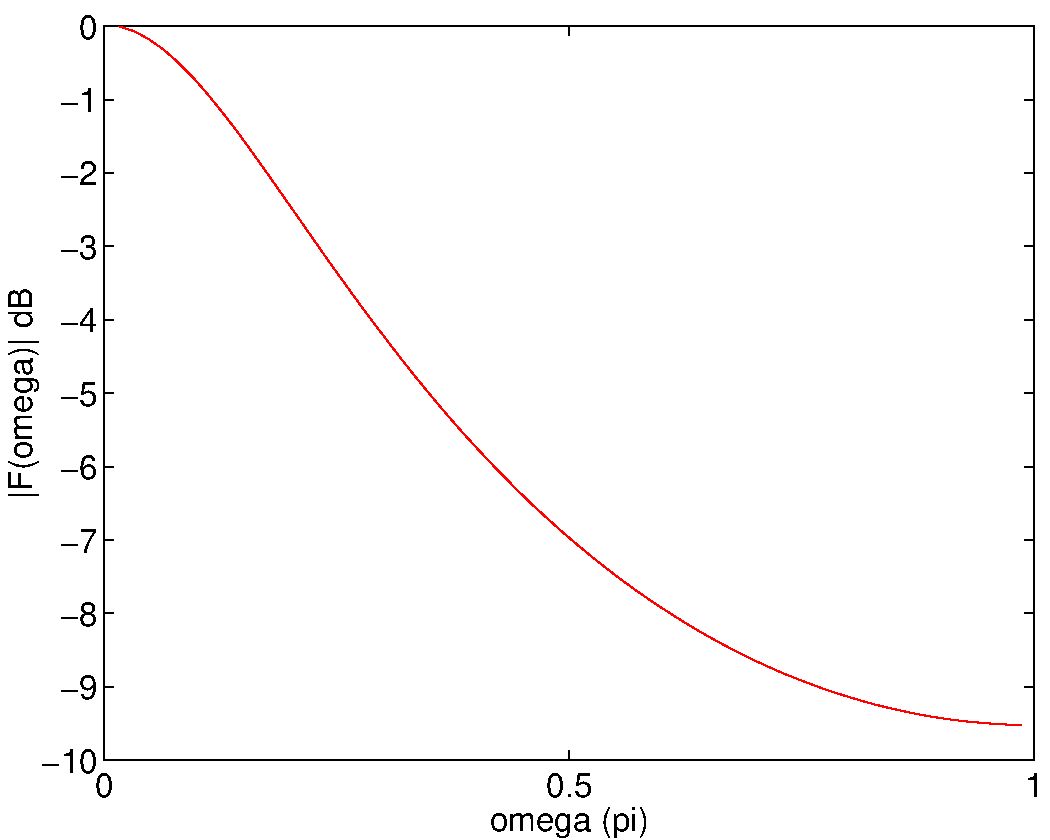
\includegraphics[width=2.5in]{ch-conv/zt_expo_r0-5F}}
\caption{Frequency content of the signal shown
in figure~\protect\ref{fig:zt-expo-r0.5f}.
\label{fig:zt-expo-r0.5F}}
\end{figure}

Figure~\ref{fig:zt-expo-r0.5F} is the plot of
$|\mathcal{X}(\hat{\omega})|$ versus frequency $\omega$.  The
amplitude decreases along increasing frequency. Its peak is at zero
frequency, which is called \emph{DC} (which literally means ``direct
current,'' implying the constant --- actually mean --- component of
the signal).

\paragraph*{When $\alpha=1$:}

For $\alpha=1$, the sequence becomes
\begin{equation}
x[n] = u[n] = \left\{\begin{array}{ll}
                        1 & n \ge 0 \\
                        0 & n < 0
          \end{array}\right.
\end{equation}
or
\begin{equation}
u[n] = \{1, 1, 1, \ldots\}, \quad k \ge 0
\end{equation}

\index{unit step}
This is a discrete time, infinite duration \emph{unit step}
signal. Notice the difference between the unit step signal and the
unit impulse signal. The latter only has one nonzero value at one
particular time, the former has value one for all time after some
particular time. By analogy with $\delta[n]$ , a unit step occurring at
sample $k$ is called $u[n-k]$.  Substituting $\alpha=1$
into~(\ref{eq:zt-expoF}) we have
\index{z-transform!of a unit step}
\begin{equation}
U(z)=\frac{1}{1-z^{-1}}, \quad |z|>1
\end{equation}
We can see that the pole (a zero in the denominator; you'll learn more
about this in Chapter~\ref{ch:fb-filters}) is at $z=1$, where the
z-transform has an infinite value.

Let's evaluate the frequency content of the unit step signal. If we
evaluate $\mathcal{U}(\hat{\omega})$ on the unit circle (except at
$z=1$), we obtain
\begin{align}
\mathcal{U}(\hat{\omega})
&= U(e^{j\hat{\omega}})
  =\frac{1}{1-e^{-j\hat{\omega}}}\frac{e^{j\hat{\omega}/2}}{e^{j\hat{\omega}/2}}
\notag\\
&= \frac{e^{j\hat{\omega}/2}}{e^{j\hat{\omega}/2}-e^{-j\hat{\omega}/2}} \notag\\
&= \frac{e^{j\hat{\omega}/2}}{2j\sin\hat{\omega}/2} \notag\\
&= \frac{e^{j(\hat{\omega}/2-\pi/2)}}{2\sin\hat{\omega}/2}, \quad \hat{\omega}\ne
2\pi k, k=0,1,\ldots
\end{align}
because $-j=e^{-j\pi/2}$ (see the self-test exercises).  Hence, the
presence of a pole (a zero in the denominator) at $z=1$ (that is, at
$\hat{\omega}=0$) creates a problem only when we want to compute
$|\mathcal{U}(\hat{\omega})|$ at $\hat{\omega}=0$, because
$|\mathcal{U}(\hat{\omega})|\rightarrow \infty$ as
$\hat{\omega}\rightarrow 0$. For any other value of $\hat{\omega}$,
$|\mathcal{U}(\hat{\omega})|$ is finite.

\begin{figure}
\centerline{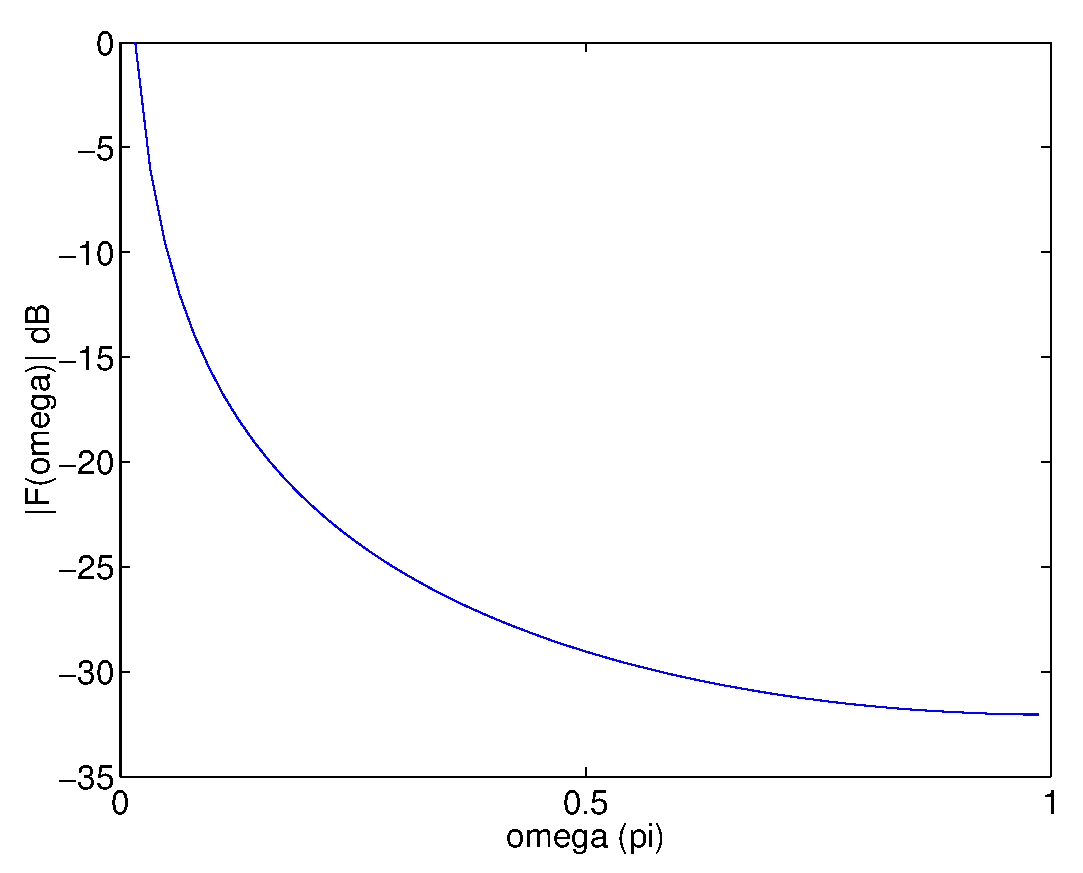
\includegraphics[width=3.5in]{ch-conv/zt_expo_r1F}}
\caption{Frequency content of the unit step signal.
\label{fig:zt-expo-r1F}}
\end{figure}

Figure~\ref{fig:zt-expo-r1F} shows a plot of
$|\mathcal{U}(\hat{\omega})|$ vs.  $\hat{\omega}$.  Since the signal
is a unit step, and so has a constant value from zero onwards, we
might expect the signal to have zero frequency components at all
frequencies except at $\hat{\omega}=0$, but that is not the case. The
reason is that the signal is not a constant for all $-\infty <n<
\infty$. Instead, it is turned on at $n=0$. This \emph{abrupt jump}
creates all the frequency components existing in the range
$0<\hat{\omega}\le\pi$. Generally, \emph{all} signals which start at a
finite time will have nonzero frequency components everywhere in the
frequency axis from zero up to the Nyquist frequency. All such signals
can be considered to be the product of some infinite signal with a
unit step; we will see the effect of this on their spectrum when we
explore convolution in section~\ref{sc:convolution}.

\paragraph*{\textsc{Optional:} When $\alpha$ is a complex number, $\alpha=Re^{j\theta}$:}

When $\alpha=Re^{j\theta}$, equations~(\ref{eq:zt-expof})
and~(\ref{eq:zt-expoF}) become
\begin{equation}
x[n] = \left\{\begin{array}{ll}
                        R^ke^{jn\theta} & \quad  n \ge 0 \\
                        0             & \quad n < 0
          \end{array}\right.
\end{equation}

\begin{equation}
X(z)=\frac{1}{1-Re^{j\theta}z^{-1}}, \quad |z|>|R|
\label{eq:zt-expo-cF}
\end{equation}

When $z=Re^{j\theta}$ we have what we call a \emph{pole} (a zero in the
denominator; you'll learn more about this in
Chapter~\ref{ch:fb-filters}). Equation~(\ref{eq:zt-expo-cF}) can be
broken into real and imaginary parts using Euler's formula:
\begin{align}
X(z) &= \frac{1}{1-Re^{j\theta}z^{-1}} \notag\\
     &= \frac{1}{1-R(\cos\theta+j \sin\theta )z^{-1}} \notag\\
     &= \frac{1}{1-R\cos\theta z^{-1}-j R\sin\theta z^{-1}} \notag\\
     &= \frac{1-R\cos\theta z^{-1}+j R\sin\theta z^{-1}}
     {[1-R\cos\theta z^{-1}]^2 - [jR\sin\theta z^{-1}]^2} \notag\\
     &= \frac{1-R\cos\theta z^{-1}+j R\sin\theta z^{-1}}
     {1-2R\cos\theta z^{-1} + R^2 z^{-2}} \notag\\
     &= \frac{1-R\cos\theta z^{-1}}
     {1-2R\cos\theta z^{-1} + R^2 z^{-2}}
     +j\frac{R\sin\theta z^{-1}}
     {1-2R\cos\theta z^{-1} + R^2 z^{-2}}
\end{align}

We break the signal into two parts, too:
\begin{align}
\Real\{x[n]\} &= R^n\cos(k\theta), \quad n\ge 0\\
\Imag\{x[n]\} &= R^n\sin(k\theta), \quad n\ge 0
\end{align}
From real part we get
\begin{equation}
R^n\cos(n\theta)\stackrel{\mathbf{Z}}{\longleftrightarrow} \
\frac{1-R\cos\theta z^{-1}}
{1-2R\cos\theta z^{-1} + R^2 z^{-2}}
\end{equation}
and from imaginary parts we have
\begin{equation}
R^n\sin(n\theta)\stackrel{\mathbf{Z}}{\longleftrightarrow} \
\frac{R\sin\theta z^{-1}}
{1-2R\cos\theta z^{-1} + R^2 z^{-2}}
\end{equation}

When $R<1$, $R^n\cos(n\theta)$ and $R^n\sin(n\theta)$ are damped
cosine and sine waves.

\problemset{
\subsubsection{Self-Test Exercises}

See~\ref{sc:ch6ex} \#\ref{it:ch6ex5}--\ref{it:ch6ex7} for answers.

\begin{enumerate}
\item What is the derivative of $u[n-k]$ (the unit step at time step
  $k$)?
\item Show that $e^{j\hat{\omega}/2}-e^{-j\hat{\omega}/2} =
  2j\sin\hat{\omega}/2$.
\item Prove that $e^{-j\pi/2}=-j$.
\end{enumerate}}

\section{Convolution}
\label{sc:convolution}

\index{convolution!discrete!definition} Convolution is an important
operation for implementing digital filters.  Let's first define what
convolution is. For two infinite, discrete signals $x[n]$ and $h[n]$,
the \emph{convolution} $y[n]$ of them at sample $n$ is defined as
\begin{equation}
y[n] = \sum_{k=-\infty}^{\infty} h[k] x[n-k]
\label{eq:convolution}
\end{equation}
The notation for convolution is ``$\ast$'', so this can be written as 
\begin{equation}
Y = X \ast H
\end{equation}
where $Y$, $X$, and $H$ are the signals with samples at $n$ being
$y[n]$, $x[n]$, and $h[n]$.

Let's consider the case when both $x$ and $h$ both start at zero. This
is equivalent to saying that both have values of zero before that
sample. So, $h[k] = 0$ when $k<0$ and $x[n-k]=0$ when
$n-k<0$. Equation~(\ref{eq:convolution}) becomes
\begin{equation}
y[n] = \sum_{k=0}^{n} h[k] x[n-k]
\label{eq:zt-conv}
\end{equation}
Actually, this is a more realistic situation than $k$'s summation
from $-\infty$ to $\infty$.

We expand the summation in~(\ref{eq:zt-conv}) as
\begin{multline}
y[n] = h[0] x[n] + h[1] x[n-1] + h[2] x[n-2] + \ldots + h[k] x[n-k]
       + \ldots \\
       {}+ h[n-2] x[2] + h[n-1] x[1] + h[n] x[0]
\label{eq:zt-conv-exp}
\end{multline}
Using this formulation, you may show that the convolution $X \ast H$ has the
following properties:
\begin{enumerate}
\item Commutative: $X \ast H=H \ast X$
\index{convolution!commutative property}
\item Distributive :  $X \ast (H_1 + H_2)=X \ast H_1 + X \ast H_2$
\index{convolution!distributive property}
\item Associative : $(X \ast H) \ast G = X \ast (H \ast G)$
\index{convolution!associative property}
\end{enumerate}
You should be able to convince yourself that $x \ast \vec{0} = \vec{0}
\ast x = 0$ (where $\vec{0}$ is a vector of all zeros). How about
$\vec{1} \ast \vec{1}$ (where $\vec{1}$ is a vector of all ones, in
this case $\vec{1}=u[n]$; see the self-test exercise)?

\subsection{Example of Convolution}

Determine the convolution $e^n \ast e^n$, $n=0,1,2,\ldots,
$. Using~(\ref{eq:zt-conv}),
\begin{align}
e^n \ast e^n &= \sum_{k=0}^{n}e^ke^{n-k} \notag\\
             &= \sum_{k=0}^{n}e^n=e^n\sum_{k=0}^{n}1=ne^n
\end{align}

\problemset{
\subsubsection{Self-Test Exercises}

See~\ref{sc:ch6ex} \#\ref{it:ch6ex8}--\ref{it:ch6ex9} for answers.

\begin{enumerate}
\item Determine if $u[n] \ast H \ne H$ is true, where $h[n] = n$,
$n=0,1,2,\ldots$ (a \emph{ramp}).
\item Compute $u[n] \ast u[n]$.
\end{enumerate}}

\subsection{Implementing Convolution}

\index{convolution!discrete!implementation}
From observation of equation~(\ref{eq:zt-conv-exp}), we know that for
a fixed sample $n$, $y[n]$ can be computed by the term-by-term
multiplication of the sequence
\begin{equation}
\{h[0], h[1], h[2], \ldots, h[k], \ldots, h[n-2], h[n-1], h[n]\}
\end{equation}
and the time-reversed sequence
\begin{equation}
\{x[n], x[n-1], x[n-2], \ldots, x[n-k] , \ldots, x[2], x[1], x[0]\}
\end{equation}
We just multiply the corresponding terms (for example, $h[k]x[n-k]$),
then add these products. This produces the convolution for one sample
$n$.  Remember, however, that the output $y[n]$ is also a sequence,
$n=0,1,2,\ldots$. We need to repeat this process for all $\{n\}$ to
get the full sequence, as shown in algorithm~\ref{alg:convolution}.
 
\begin{algorithm}
\caption{Discrete convolution.\label{alg:convolution}}
\begin{algorithmic}
\REQUIRE $h[n]$ is a finite, discrete signal, $n = 0, 1, 2, \ldots$
\REQUIRE $x[n]$ is a finite, discrete signal, $n = 0, 1, 2, \ldots$
\ENSURE $y[n]$ is the convolution $X * H$, $n = 0, 1, 2, \ldots$
\FOR{$n=0, 1, 2, \ldots$}
   \STATE Reverse $x[k]$ to produce $x'[k] = x[n-k]$, $k = 0, 1, 2,
          \ldots, n$
   \STATE $s[k] = h[k] x'[k]$
   \STATE $y[n] = \sum_{k=0}^n s[k]$
\ENDFOR
\end{algorithmic}
\end{algorithm}

A more-or-less direct implementation of this algorithm in C is:

\index{C code!convolution|(}
\begin{small}
\begin{verbatim}
/* Convolution of two vectors

   Input: vectors x and h of lengths nx and nh (nh < nx)
   Output: vector y of length nx + nh - 1 (storage already allocated)
 */
void convolve(int x[], unsigned nx, int h[], unsigned nh, int y[])
{
   for (unsigned n=0; n<nx+nh-1; n++) {
      y[n] = 0;
      for (unsigned k=max(0,n-nh+1); k<=min(nx-1,n); k++)
         y[n] += x[k] * h[n-k];
   }
}
\end{verbatim}
\end{small}
\index{C code!convolution|)}

\begin{figure}
\centerline{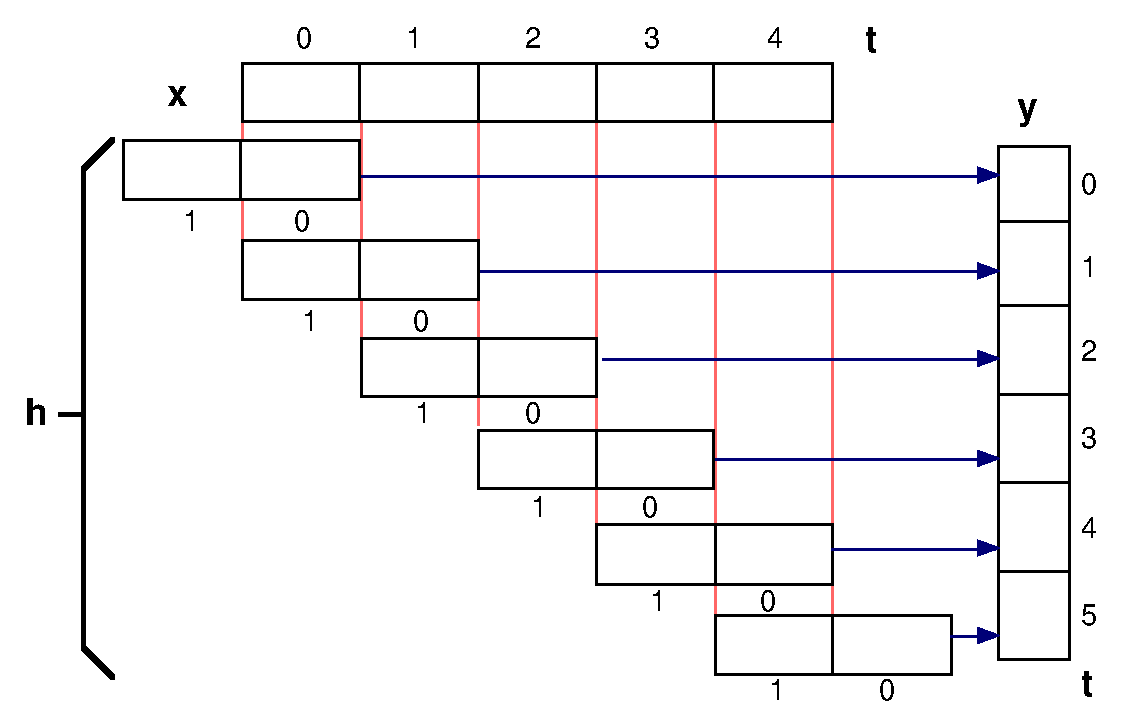
\includegraphics[width=\textwidth]{ch-conv/fig6-5}}
\caption{Example of convolution function execution for $n_x=5$ and
$n_h=2$.\label{fg:convex}}
\end{figure}

You'll notice something nasty was done here: the identities of
$x$ and $h$ were reversed! Of course, this is perfectly OK, given the commutative
property of convolution. This was done because we generally assume that $h$
(the shorter vector) is a property of the filter (we will see about
this later) and it is easier to think about reversing
it than reversing the signal $x$. If for no other reason, this makes
sense because $h$ has a shorter length.

The implementation is for finite-length signals, rather than the
infinite ones we've been discussing. It assumes that $h$ is shorter
than $x$ ($n_h < n_x$). This $h$ input is often called the convolution
\emph{kernel} because, as we shall see, $h$ represents the
\index{convolution!kernel}
action of our signal processing system while $x$ is the actual input
signal.  Notice that, for small $n<n_h-1$, not all of $h$ is
used. This is equivalent to multiplying the unused elements of $h$
against the zero values of $x[k]$, $k<0$. Similarly, for large
$n>nx-1$, part of $h$ is also unused --- multiplied against the zero
values of $x[k]$, $k>n_x-1$. Figure~\ref{fg:convex} illustrates
function execution for a signal $X$ of length 5 and a kernel $H$ of
length 2. This is one way to deal with the \emph{boundary conditions}
\index{convolution!boundary conditions}
associated with the convolution: what to do at the ends of the
signal $X$.  In general, there are three ways of dealing with these
boundary conditions:
\begin{enumerate}
\item ``Pad'' $X$ with zeros past its ends. In effect, this is what
was done in the code above.
\item ``Reflect'' $X$ by copying element $k$ to index $-k$. This is
sometimes done in image processing operations.
\item ``Truncate'' the convolution at the ends of $X$. This means that
$n$ would cover the range $n_h-1 \leq n \leq n_x$ and $Y$ would be
shorter than $X$.
\end{enumerate}

\index{MATLAB code!convolution}
MATLAB has the built-in convolution function \verb|conv|, which takes
two vectors as inputs and outputs the convolution result with length
equal to one less than the sum of the two input vector lengths. You
can use ``\verb|help conv|'' to get more information (how does
\verb|conv| deal with boundary conditions [answer in~\ref{sc:ch6ex}
\#\ref{it:ch6ex10}]?)

\begin{figure}
\centerline{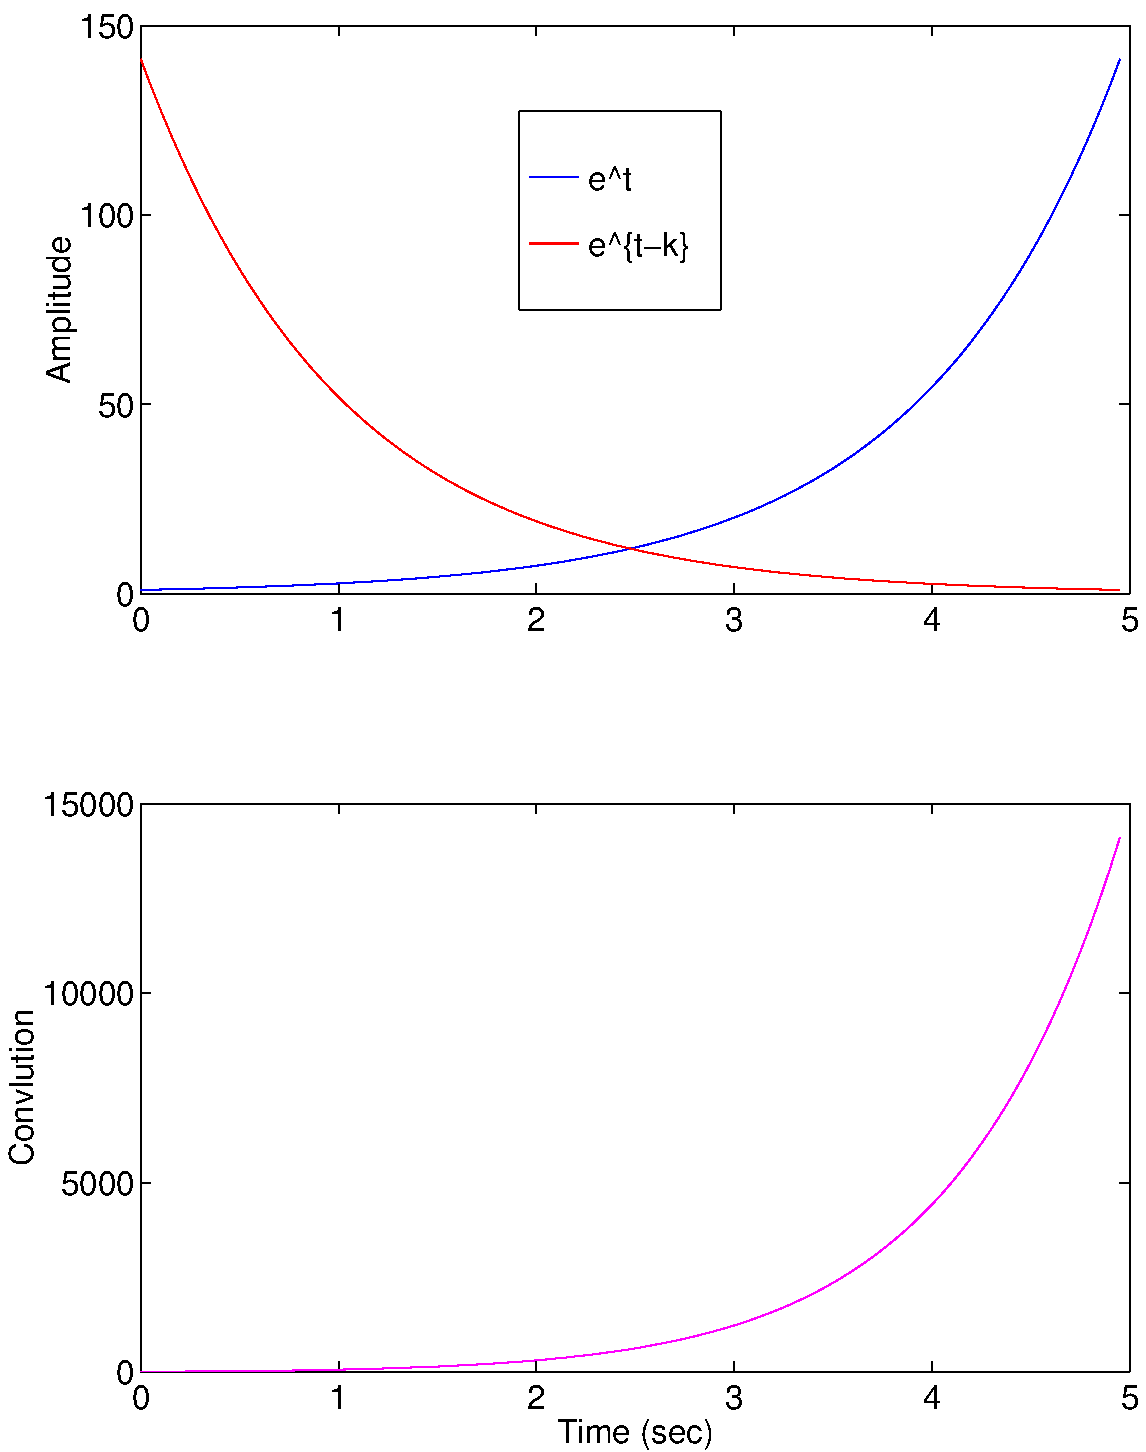
\includegraphics[width=4in]{ch-conv/zt_conv_etet}}
\caption[Convolution of $e^n \ast e^n$]{Convolution of $e^n \ast
  e^n$. Top blue line is $e^n$, top red line is time reversed version
  of $e^n$, the bottom plot is the result of convolution.
  \label{fig:zt-conv-etet}}
\end{figure}

Let's look at the convolution of $X \ast H =e^n \ast e^n$ again. In
this case, $X$ and $H$ are the same function. In
figure~\ref{fig:zt-conv-etet} (top), $X$ is shown as a blue curve and
the time-reversed $H$ is shown as a red curve. The convolution result
is in the bottom graph.

\problemset{
\subsubsection{Self-Test Exercises}

See~\ref{sc:ch6ex} \#\ref{it:ch6ex11} for the answer.

\begin{enumerate}
\item Use MATLAB to compute the convolution $e^{-n}*e^{-n}$ and plot
the result.
\end{enumerate}}

\section{Properties of the Z-Transform}

\index{z-transform!properties of}
\begin{table}
\caption{Some properties of the z-transform.\label{tb:zt-property}}
\begin{center}
\begin{tabular}{|l|c|c|} \hline
Property      & Time Domain, $Z^{-1}\{\cdot\}$ & z-Domain, $Z\{\cdot\}$ \\ \hline\hline
Linearity     & $a_1x[n]+a_2y[n]$ & $a_1X(z)+a_2Y(z)$\\ 
Time shift    & $x[n-k]$       & $z^{-k}X(z)$\\ 
Scaling in the z-domain 
              & $a^nx[n]$        & $X(a^{-1}z)$ \\ 
Time reversal & $x[-n]$        & $X(z^{-1})$\\ 
Differentiation in the z-domain 
              & $nx[n]$          & $-z \deriv{X(z)}{z}$ \\ 
Convolution   & $x[n] \ast y[n]$       & $X(z)Y(z)$ \\ \hline
\end{tabular}
\end{center}
\end{table}

The z-transform is a very powerful signal processing tool because it
has some very important properties. Some of these properties are
listed in
table~\ref{tb:zt-property}, where the time-domain signals $x[k]$
and $y[k]$ have z-transforms of $X(z)$ and $Y(z)$.

Knowing these properties can be very convenient. For example, the
z-transform of a signal shifted (delayed) by $k$ samples, $x[n-k]$,
is $z^{-k}X(z)$; this is our familiar $z$ (delay) operator. You can
\index{z-transform!relation to $z$ operator}
\index{z-transform!and delay}
also see that the convolution property of the z-transform means that
convolution in the time domain is multiplication in the z-domain. So,
if we have the z-transform of two signals, it is much easier to
perform convolution.  Later on, you will find out that this is very
important in filtering. Let's prove this property:

From~(\ref{eq:zt-conv}) a convolution of $x[n]$ and $h[n]$ is defined as:
\begin{equation}
y[n] = x[n] \ast h[n] = \sum_{k=-\infty}^{\infty} h[k] x[n-k]
\end{equation}
The z-transform of $y[n]$ is 
\begin{align}
Y(z) &= \sum_{n=-\infty}^{\infty} y[n]z^{-n} \notag\\
     &= \sum_{n=-\infty}^{\infty}
     \left( \sum_{k=-\infty}^{\infty} h[k] x[n-k] \right)z^{-n}
\end{align}
Interchanging the order of the summations (which is equivalent to
factoring out the $h[k]$ and distributing the $z^{-n}$ over the inner
summation),
\begin{equation}
Y(z) = \sum_{k=-\infty}^{\infty} h[k]
             \left( \sum_{n=-\infty}^{\infty} x[n-k] z^{-n} \right)
\end{equation}
The inner summation is merely the z-transform of $x[n]$ shifted by $k$
samples.  Applying the time shift property of the z-transform, we
obtain
\begin{align}
Y(z) &= \sum_{k=-\infty}^{\infty} h[k] X(z) z^{-k} \notag\\
     &= X(z)\sum_{k=-\infty}^{\infty} h[k] z^{-k} 
     = X(z) H(z)
\end{align}
Which is the product of the two z-transforms. I'll present a couple
examples of using these properties.

\subsection{Example: Time Shifting}

\index{z-transform!of a time-shifted impulse}
Remember that the z-transform of the unit impulse
$\delta[n]$ was discussed in section~\ref{sc:zx-impulse}
\begin{equation}
\delta[n] = \left\{\begin{array}{ll}
                        1 & n=0 \\
                        0 & n \neq 0
          \end{array}\right.
\end{equation}
as being 1 and that the z-transform of the shifted unit impulse
$\delta[n-k]$ is $z^{-k}$? Using the time-shifting property of the
z-transform, this is easy to determine:
\begin{equation}
\delta[n]\stackrel{\mathbf{Z}}{\longleftrightarrow} 1
\end{equation}
then 
\begin{equation}
\delta[n-k]\stackrel{\mathbf{Z}}{\longleftrightarrow} 1 \times z^{-k}=z^{-k}
\end{equation}

\subsection{Example: Convolution}

\index{z-transform!computing convolution with}
Given the signals 
\begin{equation}
x[n] = \{1, -3, 2, 1\}, \quad n = 0,1,2,3
\end{equation}
and 
\begin{equation}
h[n] = \left\{\begin{array}{ll}
                        1 &  n=0,1\\
                        0 &  n=2,3
          \end{array}\right.
\end{equation}
use the z-transform to compute their convolution $Y = X \ast H$.

According to~(\ref{eq:zt}),
\begin{align}
X(z) &= 1-3z^{-1}+2z^{-2}+z^{-3}\\
H(z) &= 1+z^{-1}
\end{align}
Then using the convolution property of the z-transform, we have 
\begin{align}
Y(z)=X(z)H(z)
&= (1-3z^{-1}+2z^{-2}+z^{-3})(1+z^{-1}) \notag\\
&= 1-2z^{-1}-z^{-2}+3z^{-3}+z^{-4}
\end{align}
Now we can easily get the inverse z-transform $y[n]=x[n] \ast h[n]$ from the
result $Y(z)$. Again from the z-transform
definition~(\ref{eq:zt}),
\begin{equation}
y[n] = x[n] \ast h[n] = \{1,-2, -1, 3, 1\}
\end{equation}

We can also compute the convolution directly, according to the
convolution definition~(\ref{eq:zt-conv}). There are only 4 nonzero
terms in $x[n]$ and 2 in $h[n]$. For a fixed sample $n$, the
convolution is given by
\begin{align}
y[n] &= \sum_{k=0}^{n} x[k] h[n-k] \notag\\
     &= x[0] h[n] + x[1] h[n-1] + x[2] h[n-2] + x[3] h[n-3]
\end{align}
Changing $n$ gives the sequence of the convolution output as a
function of time. In the following computation, $h[n-k]=0$ is used,
if $n-k<0$ and $x[k]=0$ and $h[k]=0$ if $k>3$:
\begin{align*}
y[0] &= x[0] h[0] = 1\\
y[1] &= x[0] h[1] + x[1] h[0] = 1-3 = -2\\
y[2] &= x[0] h[2] + x[1] h[1] + x[2] h[0] = 0-3+2 = -1\\
y[3] &= x[0] h[3] + x[1] h[2] + x[2] h[1] +x[3] h[0] = 0+0+2+1 = 3\\
y[4] &= x[1] h[3] + x[2] h[2] + x[3] h[1] = 0+0+1 = 1\\
y[n] &= 0, \quad n>4
\end{align*}
Therefore, this also gives the result
\begin{equation}
y[n] = x[n] \ast h[n] = \{1,-2, -1, 3, 1\}
\end{equation}

\problemset{
\subsubsection{Self-Test Exercises}

See~\ref{sc:ch6ex} \#\ref{it:ch6ex12} for the answer.

\begin{enumerate}
\item Prove the scaling property of the z-transform; that is, if 
  \begin{equation*}
    x[n]\stackrel{\mathbf{Z}}{\longleftrightarrow} X(z)
  \end{equation*}
  then 
  \begin{equation*}
    a^n x[n]\stackrel{\mathbf{Z}}{\longleftrightarrow} X(a^{-1}z)
  \end{equation*}
\end{enumerate}}

\section{Impulse Response and the Transfer Function}

Recall the a filter's input/output relationship is summarized by the
transfer function discussed in chapter~\ref{ch:filt-intro} (and which
you'll see again in chapter~\ref{ch:fb-filters}). Let's denote the
input signal as $x[n]$ and output as $y[n]$ in the time domain. You
learned that the the transfer function in the z domain is $H(z)$. What
is its time domain representation? We will answer this shortly; first
let's give a name to the time domain transfer function,
$h[n]$: the filter's
\emph{impulse response}. The filter's input/output relationship can be
\index{filter!impulse response}
written using $h[n]$ as:
\begin{equation}
y[n] = x[n] \ast h[n]
\label{eq:zt-hx}
\end{equation}
This says that the output of filter results from the convolution
between input signal $x[n]$ and filter's impulse response $h[n]$. From
earlier in this chapter, you now know that convolution of two signals
in the time domain is equivalent to multiplying their z-transforms in
the $z$ domain. So, we obtain the input/output relationship via the
transfer function in the $z$ domain as
\begin{equation}
Y(z) =X(z)H(z)
\label{eq:zt-HX}
\end{equation}
where $X(z)$ and $Y(z)$ are the z-transforms of $x[n]$ and $y[n]$ and
$H(z)$ is the z-transform of $h[n]$.  Actually, this $H(z)$ is just
the transfer function we talked about in chapter~\ref{ch:filt-intro}.
In other words, a filter's transfer function is the z-transform of its
impulse response!
\index{z-transform!relationship to filter transfer function}
\index{filter!transfer function!relationship to its z-transform}

\index{filter!transfer function!determining with z-transform}
As a simple example of how to use the z-transform to determine a
filter's transfer function from its defining equation, consider the
feedforward filter:
\begin{equation}
y[n] = b_0x[n] + b_1x[n-k]
\end{equation}

Applying the z-transform to both sides, 
\begin{equation}
Y(z) = b_0X(z) + b_1z^{-k}X(z)
\end{equation}
because of the time shift property of the z-transform. This can be
rearranged to be
\begin{equation}
Y(z) = (b_0 + b_1z^{-k})X(z)
\end{equation}
So the transfer function is 
\begin{equation}
H(z) = b_0 + b_1z^{-k}
\end{equation}
and therefore, we have
\begin{equation}
Y(z)=H(z)X(z)
\end{equation} 

Applying the inverse z-transform, we can get the time domain
representation of $H(z)$, or the impulse response $h[n]$. In a similar
manner, we can get the output $y[n]$ from $Y(z)$.  In fact,
using~(\ref{eq:zt-HX}), we found an easy way to compute a filter's
response to a signal if we have already know the signal's z-transform
and the filter's transfer function.

Let's see why $h[n]$ is called the impulse response.  Remember the unit
impulse, which is a signal that has the value one at $n=0$ and zero
otherwise, and which can be expressed as
\begin{equation}
\delta[n] = \left\{\begin{array}{ll}
                        1 & n=0 \\
                        0 & n \neq 0
          \end{array}\right.
\end{equation}

The impulse response of a filter is its output when a unit impulse is
applied. Now we compute these two functions' convolution,
\begin{equation}
y[n]=\sum_{k=0}^{n}\delta[k] h[n-k] = h[n]
\end{equation}
because all of the terms except $k=0$ drop out (since $\delta[k]=0$
for all $k \ne 0$).  This tell us that the filter response $y[n]$ to a
unit impulse is $h[n]$. This is why $h[n]$ is called the impulse
response.

Applying the z-transform to both side of the above equation, we get
\begin{equation}
Y(z)= H(z)
\end{equation}
Therefore, the \emph{transfer function} can be viewed as the
z-transform of the filter's \emph{impulse response}, or its impulse
response in the $z$ domain.

If we restrict $z$ to lie on the unit circle, $z=e^{j\hat{\omega}}$,
from~(\ref{eq:zt-HX}) we obtain
\begin{equation}
\mathcal{Y}(\hat{\omega})=\mathcal{H}(\hat{\omega})\mathcal{X}(\hat{\omega})
\end{equation} 
where $\mathcal{X}(\hat{\omega})$ is the signal's frequency content,
$\mathcal{Y}(\hat{\omega})$ is the frequency content of the filter
output and $\mathcal{H}(\hat{\omega})$ is the filter's frequency
response.


\section{Problems}

\begin{enumerate}
\item Compute the z-transform of 
\begin{equation}
x[n] = \left\{\begin{array}{ll}
                        (-1)^n & n \ge 0 \\
                        0 & n < 0
          \end{array}\right.
\end{equation}
and determine its frequency content. 

\item Determine the z-transform of the signal 
\begin{equation}
x[n] = \left\{\begin{array}{ll}
                        \cos\hat{\omega}_0 n & n \ge 0 \\
                        0 & n < 0
          \end{array}\right.
\end{equation}

\item Find the z-transform of the signal
\[x[n] = \left\{\begin{array}{ll} 1/n! & n \geq 0 \\
                0 & n < 0 \end{array} \right. \]
Recall that $0!=1$.

\item The impulse response of a system is $h[n]=\{1,2,1,-1\}$, $n=-1,
0,1,2$. Determine the response of the system to the input signal
$x[n]=\{1,2,3,1\}$, $n=0, 1,2,3$.

\end{enumerate}


\section{Further Reading}

\begin{itemize}
\item James H McClellan, Ronald W. Schafer, and Mark A. Yoder,
  \textit{DSP First: A Multimedia Approach}, Prentice Hall, 1998,
  chapter 7 (\S 7.1--7.6.3).
\end{itemize}

% LocalWords:  DTFT signal's feedforward

% -*-LaTeX-*-

% $Log: fb-filters.tex,v $
% Revision 1.7  2007/12/25 17:47:12  stiber
% Some final cosmetic changes.
%
% Revision 1.6  2007/12/11 17:49:03  stiber
% Small changes to get ready for Witner 2008.
%
% Revision 1.5  2007/03/20 23:53:48  stiber
% Updated eqnarray to align.
%
% Revision 1.4  2007/03/20 18:14:34  stiber
% Modified for use as part of standalone text.
%
% Revision 1.3  2006/03/27 23:37:41  stiber
% Fixed errors in formulas; deleted end-of-chapter problem that lacked
% prerequisite material upon switching of textbook.
%
% Revision 1.2  2004/03/29 19:54:44  stiber
% Updated for Spring 2004 and new textbook (DSP First).
%
% Revision 1.1  2004/02/19 00:24:45  stiber
% Initial revision
%

\chapter{Feedback Filters}
\label{ch:fb-filters}

\section{Introduction}

In this chapter, we will continue to introduce filters, this chapter
focusing on \emph{feedback filters}, in which previous outputs are
combined with new inputs to produce new outputs. We will learn about
their structure, function, and the differences between feedforward and
feedback filters.  We will see that sometimes it is better to combine
these two kinds of filters. We will also briefly examine digital
filter design. After this chapter, you should understand important
concepts like the \emph{poles} (as compared to \emph{zeros}) of a
transfer function, \emph{impulse response}, and \emph{bandwidth}. You
should know about features of feedback filters and special types of
such filters, such as \emph{resons}.  You should be able to design
simple digital filters, implement them on a computer and use them to
solve some simple signal processing problems.

\subsection{Poles}

\begin{figure}
\centerline{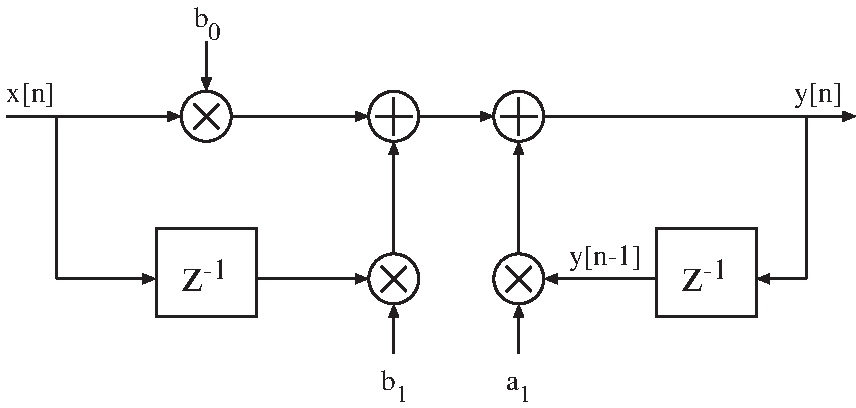
\includegraphics[width=0.5\textwidth]{ch-iir/fb-bdiag}}
\caption{Block diagram of a simple filter with both feedforward and
  feedback terms.\label{fig:fb-bdiag}}
\end{figure}

Figure~\ref{fig:fb-bdiag} presents the block diagram of a filter with
one feedforward and one feedback term; the feedback filter's signal
flowgraph is shown on the right. Compared to the feedforward one on
the left in the figure, we notice that instead of combining the input
signal with a delayed version, here the output signal is delayed and
``fed back'' to be combined with the input. The feedback processing
alone is expressed by
\begin{equation}
y[n] = x[n] + a_1 y[n-1]
\label{eq:fb-1p}
\end{equation}
(ignoring the factor of $b_0$) which is the equation for a simple
feedback filter with one delayed component. $a_1 y[n-1]$ is the
feedback term. You can see that the output at $n-1$ is used to compute
the output at time $n$. The combined filter's full defining equation
is
\begin{equation}
  y[n] = b_0 x[n] + b_1 x[n-1] + a_1 y[n-1]
  \label{eq:fb-ff}
\end{equation}
but for the moment we will concentrate on just the feedback part of
the filter, from equation~(\ref{eq:fb-1p}).

From equation~(\ref{eq:fb-1p}), the z-transforms of the input and
output signals, and the delay operator $z^{-1}$, we can get the
filter's transfer function as follows:
\begin{align}
Y(z) &= X(z) + a_1z^{-1}Y(z) \notag\\
Y(z)[1-a_1z^{-1}] &= X(z) \notag\\
Y(z) &= \frac{1}{1-a_1z^{-1}}X(z)
\end{align}
Finally we have the transfer function:
\begin{align}
H(z) &= \frac{Y(z)}{X(z)} = \frac{1}{1-a_1z^{-1}} \notag \\
     &= \frac{z}{z-a_1} \label{eq:fb-xfer}
\end{align}
The magnitude response is:
\begin{equation}
|\mathcal{H}(\hat{\omega})|
  = |H(z)|
  = \left|\frac{z}{z-a_1}\right|=\left|\frac{1}{z-a_1}\right|
\label{eq:fb-1pmh}
\end{equation}
($|z|=1$ because we are only concerned with the magnitude when $z$ is
on the unit circle, and so its magnitude is always one).

\index{filter!poles|emph} The values of $z$ that make the denominator
of the transfer function zero (the roots of the denominator
polynomial, where the transfer function becomes infinite) are called
its \emph{poles}. In~(\ref{eq:fb-1pmh}), there is one pole at
$z=a_1$. In general, $a_1$ is not on the unit circle, and so the
phasor $z$ approaches it but is never equal to it.  Just as we did for
zeros, we can draw a line from the pole to the unit circle to indicate
the distance between $z$ and the pole.  However, now this distance is
in the denominator. Therefore, instead of $H(z)$ having a notch or dip
when $z$ nears a zero, it has a \emph{peak} when $z$ nears a pole.

\begin{figure}
\centerline{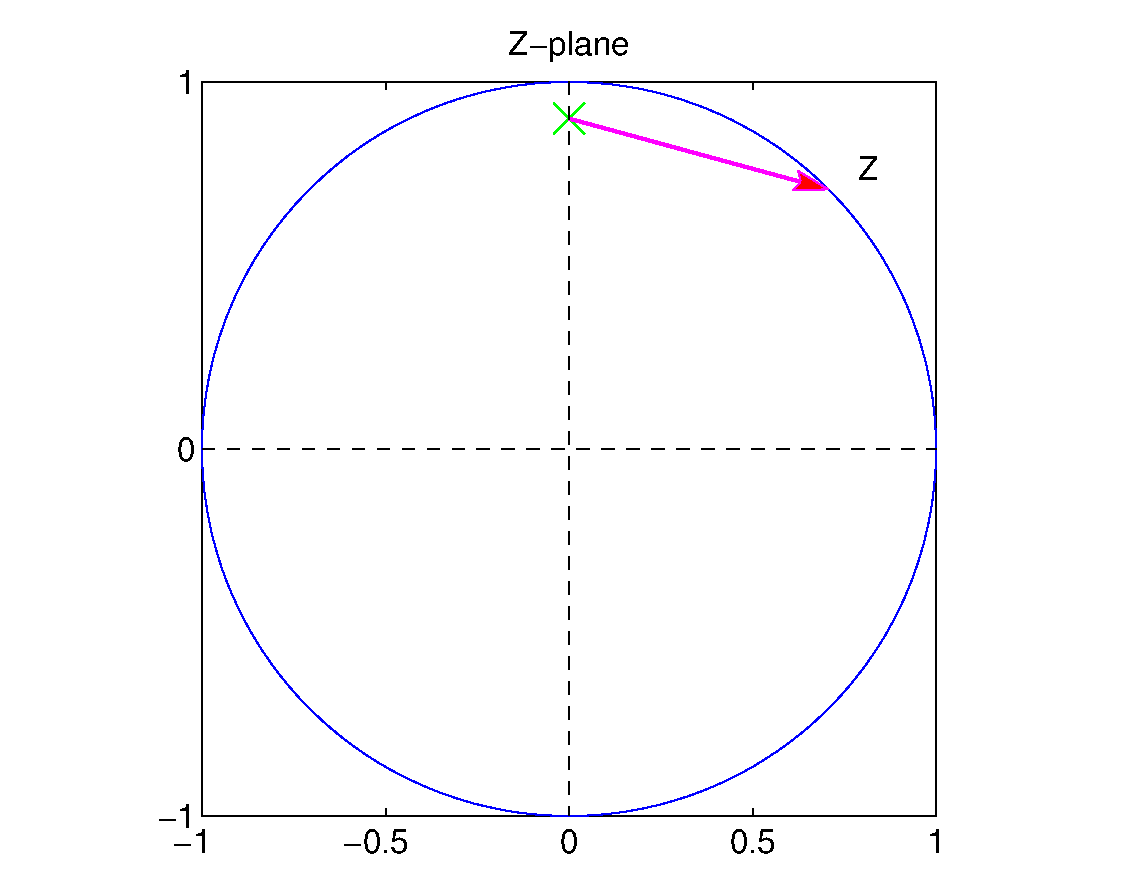
\includegraphics[height=3.5in]{ch-iir/fbexp_1p_c90}}
\caption{One pole in the $z$-plane, located at $r=0.9$ and
$\hat{\omega}_0=\pi/2$.\label{fig:fb-exp1pc90}}
\end{figure}

\begin{figure}
\centerline{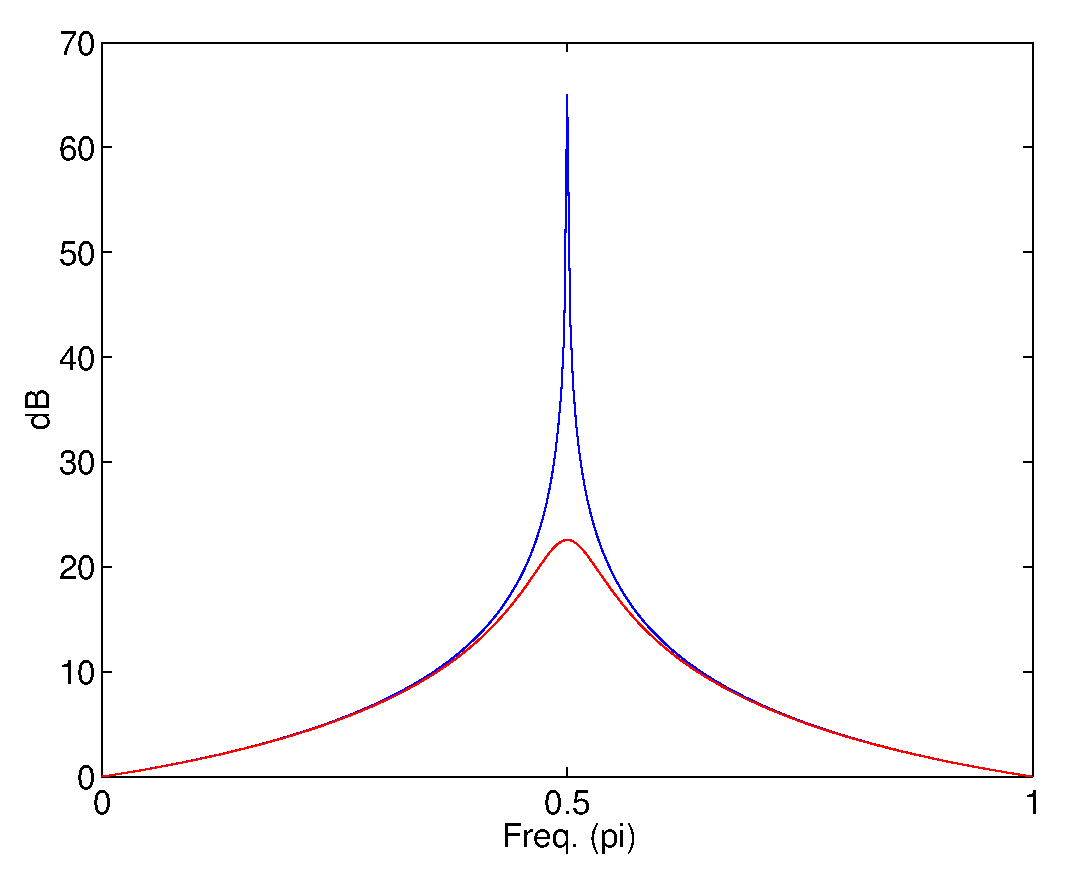
\includegraphics[height=3in]{ch-iir/fbexp_1p_h90_r1_r0-9}}
\caption[Magnitude response of two filters]{Magnitude response of two
  filters with poles located at $\hat{\omega}_0=\pi/2$ and $r=0.9$
  (bottom) or $r=1$ (top).\label{fig:fb-exp1ph90r2}}
\end{figure}

\paragraph*{Example~1} 
For the one pole filter~(\ref{eq:fb-1p}),
$a_1=re^{j\hat{\omega}_0}$. Figure~\ref{fig:fb-exp1pc90} shows this
pole when $r=0.9$ and
$\hat{\omega}_0=\pi/2$. Figure~\ref{fig:fb-exp1ph90r2} shows its
magnitude response. As expected, $|\mathcal{H}(\hat{\omega})|$ has a
``hill'' near $\hat{\omega}_0=\pi/2$. As $r$ moves closer to one, the
hill becomes steeper.

\subsection{Example: Computing Transfer Function and Impulse Response}

Compute the transfer function and impulse response of the system
described by the feedback filter, 
\begin{equation}
y[n] = 2x[n] + \frac{1}{2}y[n-1]
\end{equation}

By computing the z-transform of the both side of above equation and
using the fact that
\begin{equation}
y[n-1]\stackrel{\mathbf{Z}}{\longleftrightarrow} z^{-1}Y(z)
\end{equation}
we obtain,
\begin{equation}
Y(z)= 2X(z) + \frac{1}{2}z^{-1}Y(z).
\end{equation}
Hence the transfer function is 
\begin{equation}
H(z)= \frac{Y(z)}{X(z)} = \frac{2}{1-\frac{1}{2}z^{-1}}
    = \frac{2z}{z-\frac{1}{2}} \label{eq:fb-exxfer}
\end{equation}

$H(z)$ has a pole at $z=1/2$ and zero at $z=0$. Now we
compute its impulse response. Previously we had an example of an
exponential signal~(\ref{eq:zt-expof}) and its
z-transform~(\ref{eq:zt-expoF}), so we have
\begin{equation}
a^n\stackrel{\mathbf{Z}}{\longleftrightarrow}
\frac{1}{1-az^{-1}}, \quad n \ge 0, |z|>a
\end{equation}
This is of the same form as~(\ref{eq:fb-exxfer}), with $a=1/2$.  Using
this result, we obtain the inverse transform
\begin{equation}
h[n] = 2\left(\frac{1}{2}\right)^n, \quad n\ge 0 \label{eq:fb-eximp}
\end{equation}
where the left and right sides of equation~(\ref{eq:fb-eximp}) are the
inverse z-transforms of $H(z)$ and $2/(1-\frac{1}{2}z^{-1})$
from equation~(\ref{eq:fb-exxfer}), respectively (the latter making
use of our example from section~\ref{sc:zx-exp}).  This is the
corresponding impulse response.

\subsection{Stability}

Let's examine equation~(\ref{eq:fb-1p}) again. Note that $y[n]$
doesn't only depend on $x[n]$. This means that, even if the input
signal is zero after some initial value, this feedback term can
continue to have a nonzero value and so the filter can still produce
some output. This is a major difference from feedforward filters,
where the output depends only on the input. As an extreme example,
consider the case where the input signal is a \emph{unit impulse},
\begin{equation}
x[n] = \delta[n] =
\left\{\begin{array}{rl}
1 & n=0\\
0  & n>0
\end{array}\right.
\end{equation}
which means it only has a value of one at the beginning, and then
turns off.  The output of any filter for a unit impulse is called,
logically enough, its \emph{impulse response}.  For the filter
in~(\ref{eq:fb-1p}) with coefficient $a_1=0.5$, the impulse response
is:
\begin{align}
y[0] &= x[0] = 1 \notag\\
y[1] &= x[1] + 0.5 y[0] = 0+0.5 \times 1 = 0.5 \notag\\
y[2] &= x[2] + 0.5 y[1] = 0+0.5 \times 0.5=0.25=0.5^2 \notag\\
y[3] &= x[3] + 0.5 y[2] = 0+0.5 \times 0.25=0.125=0.5^3 \notag\\
& \vdots  \notag \\
y[n] &= 0.5^n \label{eq:fb-1pexp}\\
& \vdots  \notag
\end{align}
You can see that the output $y[n]$ continues after $n=0$, but the
value becomes smaller each time, and will decay towards zero.  On the
other hand, if $a_1>1$, the output becomes bigger and bigger, and goes
to infinity. This second behavior is called \emph{unstable}.  From
equation~(\ref{eq:fb-1pmh}), we know that $a_1$ is a pole of the
filter.  In fact, a feedback filter with multiple poles $p_i$ is
stable if and only if
\begin{equation}
|p_i| < 1,  \text{ for all } i
\end{equation}
In other words, \emph{all} the poles must be inside the unit
circle. Here is the basic idea for a four-step (well,
three-step-and-a-note) proof of this:

\begin{enumerate}
\item \textbf{A feedback filter with $N$ feedback terms can be decomposed into
$N$ one-pole feedback filters.}

\begin{figure}
\centerline{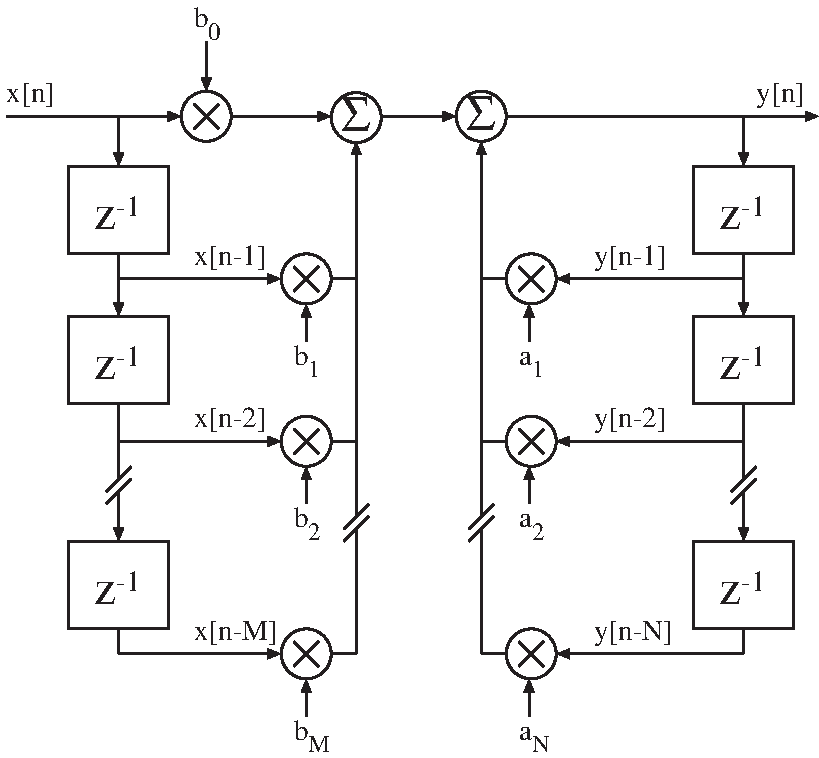
\includegraphics[width=0.5\textwidth]{ch-iir/fb-nterm-bdiag}}
\caption{Block diagram of a filter with $M$ feedforward and $N$
  feedback terms.\label{fig:fb-nterm-bdiag}}
\end{figure}

The equation for a feedback filter with $N$ feedback terms (the right
hand side of the general feedforward/feedback filter block diagram in
figure~\ref{fig:fb-nterm-bdiag}) can be written as
\begin{equation}
y[n] = x[n] - \sum_{k=1}^N a_k y[n-k]
\end{equation}
Its transfer function is 
\begin{align}
H(z) &= \frac{1}{1 + \sum_{k=1}^N a_k z^{-k}} \notag \\
     &= \frac{z^N}{z^N+\sum_{k=1}^N a_k z^{N-k}} \label{eq:manypoles}
\end{align}
where we've multiplied by $z^N/z^N$, as is our usual practice, to
produce a ratio of polynomials with positive exponents.

Let $p_i, i=1, 2,...,N$ be its poles (the roots of the denominator
polynomial). Let's not worry about how we can get them (we know how if
we can factor the denominator polynomial, so let's assume we have
already done that).  So,~(\ref{eq:manypoles}) can be rewritten in the
form
\begin{align}
H(z) &= \frac{z^N}{(z-p_1)(z-p_2)\hdots (z-p_N)}\\
     &= \frac{z^N}{\prod_{k=1}^N(z-p_k)}\label{eq:mp-denomprod}
\end{align}
Recalling our pre-calculus, a fraction with a product of terms as
in~(\ref{eq:mp-denomprod}) can be rewritten using a partial fraction
expansion as \index{partial fraction expansion}
\begin{align}
H(z) &= \frac{A_1}{(1-p_1z^{-1})}+\frac{A_2}{(1-p_2z^{-2})}+\hdots +
\frac{A_N}{(1-p_Nz^{-N})}\\
&= \sum_{k=1}^N\frac{A_k}{(1-p_k z^{-k})}
\end{align}
Each of the terms
\begin{equation}
\frac{A_k}{(1-p_k z^{-k})}
\end{equation}
is a one-pole feedback filter. So, the complete $N$-pole filter's
output is the sum of $N$ one-pole filters' outputs. This is called a
parallel one-pole filter.
\index{filter!parallel one-pole}

\item \textbf{A one-pole feedback filter is stable if and only if its
impulse response is stable.}

Consider the unit impulse $\delta[n]$,
\begin{equation}
\delta[n] = 
\left\{\begin{array}{rl}
1 & n=0\\
0 & n>0
\end{array}\right.
\end{equation}
Any discrete input signal can be thought of as a weighted sum of
delayed unit impulses. This is a straightforward application of the
knowledge that $\delta[n]=1$ when $n=0$,  $\delta[n-1]=1$  when $n=1$,
$\delta[n-2]=1$ when $n=2$, etc. Each of these is zero for all other
time indices, so we can use a sum of impulses, each multiplied by the
corresponding element of $x[n]$, to express a discrete signal:
\begin{align}
x[n] &= \{x[0], x[1], x[2], \ldots\} \notag \\
     &= x[0]\delta[n] + x[1]\delta[n-1] + x[2]\delta[n-2] + \cdots
\end{align}
We can see that the filter's response to any signal will be stable if
and only if its response to each of these impulses is stable.

\item \textbf{An impulse response is stable if and only if its pole's
$|p|<1$.}

Equation~(\ref{eq:fb-1pexp}) tell us that the \spscript{$i$}{th}
one-pole feedback filter's impulse response is the signal with samples
\begin{equation}
1, p_i, p_i^2, p_i^3, \ldots
\end{equation}
This impulse response is stable only when the pole's $|p_i|<1$, so
that the sequence is decreasing in magnitude.

\item \textbf{An impulse response is neither stable nor unstable if
$|p|=1$.}
\end{enumerate}

\subsection{Resonance and Bandwidth}

\index{filter!resonance}
\emph{Resonance} is the increase in a filter's magnitude response in
the region near a pole. An example is shown in
figure~\ref{fig:fb-exp1ph90r2}. The pole is at frequency
$\hat{\omega}=\pi/2$, which is the peak of the magnitude response. The
magnitude is small when away from the pole.

One other thing mentioned before is that the peak becomes steep
when $r$ nears one. The steepness is measured by the filter's
\emph{bandwidth}.
\index{bandwidth}
Bandwidth, $B$, is defined as the width of the
filter's response (i.e., the range of frequencies) at half its maximum
power output. Bandwidth is an important measure of a filter's
performance; it indicates which frequencies are passed and which are
filtered out.

The filter's power is the square of its amplitude, so the bandwidth
can also be measured at $1/\sqrt{2}$ of its peak amplitude value.
These half power levels are denoted by
$|\mathcal{H}(\hat{\omega})|_B^2$ (the $1/\sqrt{2}$ amplitude points
written as $|\mathcal{H}(\hat{\omega})|_B$). If the peak value of
power is $|\mathcal{H}(\hat{\omega})|_p^2$ and the peak amplitude is
$|\mathcal{H}(\hat{\omega})|_p$, the bandwidth points are located at
the (two) values of $\hat{\omega}$ that satisfy the following
relationship:
\begin{equation}
\underbrace{|\mathcal{H}(\hat{\omega})|_B}_{\stackrel{\text{cutoff}}{_\text{amplitude}}}
  = \frac{1}{2}\underbrace{|\mathcal{H}(\hat{\omega})|_p^2}_{\stackrel{\text{peak}}{_\text{power}}}
  = \frac{1}{\sqrt{2}}\underbrace{|\mathcal{H}(\hat{\omega})|_p}_{\stackrel{\text{peak}}{_\text{amplitude}}}
\label{eq:fb-band}
\end{equation}

Since $20\log_{10}(1/\sqrt{2})=-3\mathrm{dB}$
\begin{equation}
\frac{|\mathcal{H}(\hat{\omega})|_B}{|\mathcal{H}(\hat{\omega})|_p} 
  = -3\mathrm{dB}
\end{equation}
and so the \emph{cutoff amplitude} for a filter are those for which
its output is reduced $3\mathrm{dB}$ from its peak.
\index{filter!cutoff amplitude}
\index{filter!cutoff frequency}
The values of $\hat{\omega}$ at which the filter's output is reduced
by this much define the edges of its \emph{passband} and are called
its \emph{cutoff frequencies}; they are sometimes called
its ``minus three deebee points''.
\index{filter!passband}
We will call these frequencies $\hat{\omega}_B$ in the simple case
where the passband is symmetrical and the two cutoff frequencies are
the same amount above and below the frequency at peak filter output,
$\hat{\omega}_p$.

\begin{figure}
\centerline{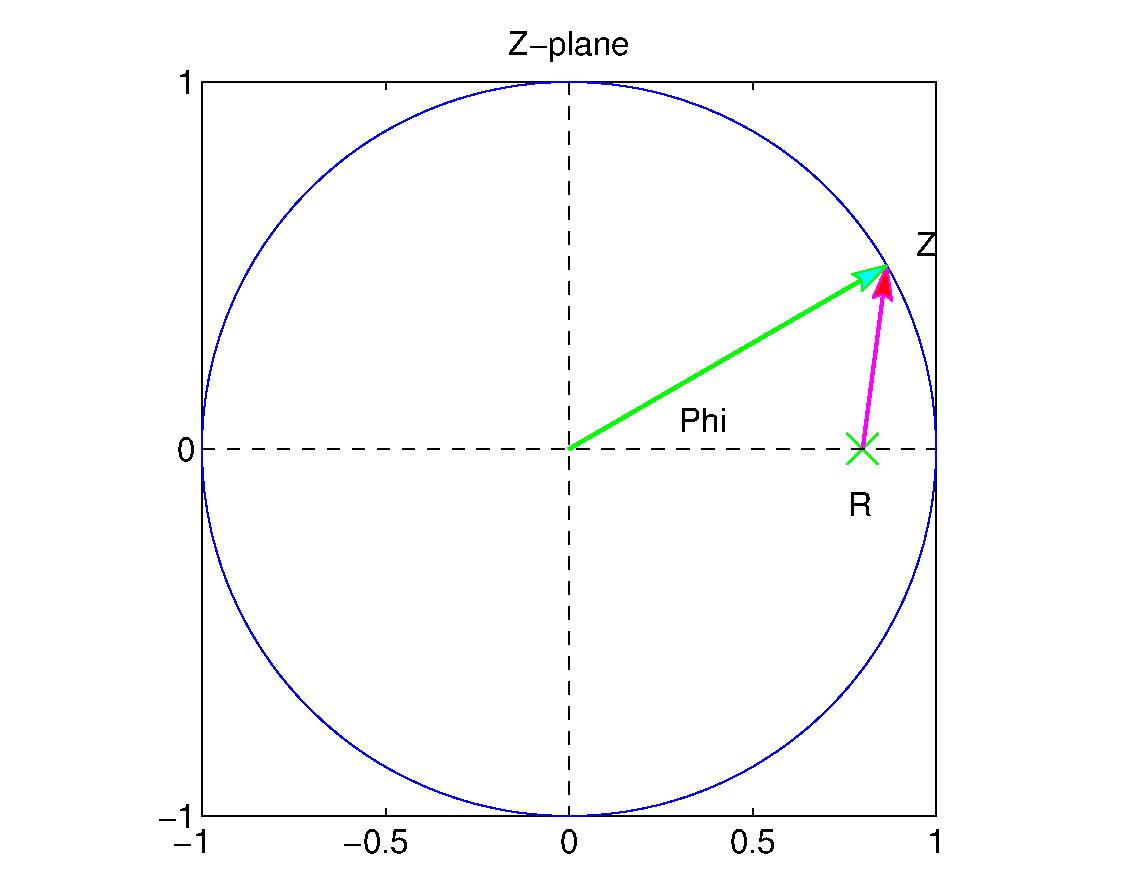
\includegraphics[height=3.5in]{ch-iir/fbexp_1p_c0_phi}}
\caption{One pole $a_1=re^{j\hat{\omega}_0}$ in z-plane. $r=R$,
$\hat{\omega}_0=0$ and $z=e^{j\hat{\omega}}$
\label{fig:fb-exp1pc0_phi}}
\end{figure}

Let's make matters simple and take a look at the case in which a pole
is on the real axis and no other poles are nearby; the pole is
$a_1=re^{j\hat{\omega}_0}$, $r=R$ and $\hat{\omega}_0=0$ (so
$a_1=R$). A point on the unit circle is $z=e^{j\hat{\omega}}$. This
situation is illustrated in figure~\ref{fig:fb-exp1pc0_phi}.  We know
that the one pole transfer function is
\begin{equation}
H(z)=\frac{1}{1-a_1z^{-1}}
\end{equation}
with magnitude 
\begin{equation}
|H(z)|=\left|\frac{1}{1-a_1z^{-1}}\right| \label{eq:reson-mag}
\end{equation}

Consider the inverse square of the magnitude, substituting in our
expressions for $a_1$ and $z$,
\begin{align}
\frac{1}{|\mathcal{H}(\hat{\omega})|^2}
    &= |1-R e^{j\hat{\omega}}|^2 \notag\\
    &= |1 - R\cos\hat{\omega} - jR\sin\hat{\omega}|^2 
    &&\text{(using Euler's formula)}
    \notag\\
    &= (1 - R\cos\hat{\omega})^2 + R^2\sin^2\hat{\omega} 
    &&\left(|H|^2 = \Real[\mathcal{H}]^2 + \Imag[\mathcal{H}]^2\right)
    \notag\\
    &= 1 - 2R\cos\hat{\omega} +R^2\cos^2\hat{\omega} +
       R^2\sin^2\hat{\omega} \notag\\ 
    &= 1-2R\cos\hat{\omega} + R^2
    &&\left(\cos^2\theta + \sin^2\theta = 1\right)
    \label{eq:reson-inv-mag2}
\end{align}
The peak of $|\mathcal{H}(\hat{\omega})|^2$ should be the value of
angle $\hat{\omega}_p=\hat{\omega}$ that makes
$1/|\mathcal{H}(\hat{\omega})|^2=1-2R\cos\hat{\omega} + R^2$ minimum
(and so $|\mathcal{H}(\hat{\omega})|^2$ maximum),
that is when $\hat{\omega}=0$. The power at this peak is determined by
substituting $\hat{\omega}=0$ into equation~(\ref{eq:reson-inv-mag2})
and taking its reciprocal:
\begin{equation}
|\mathcal{H}(\hat{\omega})|^2_p=\frac{1}{(1-R)^2}
\end{equation}
According to equation (\ref{eq:fb-band}), 
\begin{equation}
|\mathcal{H}(\hat{\omega})|_B
  =\frac{1}{2}|\mathcal{H}(\hat{\omega})|^2_p=\frac{1}{2(1-R)^2}
\end{equation}
The corresponding $\hat{\omega}_B$ can be obtained by substituting
$|\mathcal{H}(\hat{\omega})|_B$ for $|\mathcal{H}(\hat{\omega})|$ in
equation~(\ref{eq:reson-inv-mag2}) and solving for frequency:
\begin{align}
2(1-R)^2 &= 1-2R\cos\hat{\omega_B}+R^2 \label{eq:fb-band2a}\\
\cos\hat{\omega}_B &= 2-\frac{1}{2}\left(R+\frac{1}{R}\right)
\label{eq:fb-band2b}
\end{align} 

The filter's bandwidth is the span $[-\hat{\omega}_B, \hat{\omega}_B]$
--- a distance of $2\hat{\omega}_B$.  When $R$ is close to one, we can
express $R$ as a small amount $\epsilon$ less than one:
$R=1-\epsilon$. We can then take advantage of the expansions:
\begin{equation}
\frac{1}{R}=\frac{1}{1-\epsilon}=1+\epsilon+\epsilon^2+\epsilon^3+\cdots
\end{equation}
and
\begin{equation}
\cos\epsilon=1-\frac{\epsilon^2}{2!}+\frac{\epsilon^4}{4!}+\cdots
\end{equation}
So, from~(\ref{eq:fb-band2b}),
\begin{align}
\cos\hat{\omega}_B &= 2-\frac{1}{2}[\underbrace{(1-\epsilon)}_{R} +
            \underbrace{(1+\epsilon+\epsilon^2+\epsilon^3+\cdots)}_{\frac{1}{R}}]
              \notag\\
   &= 1-\frac{\epsilon^2}{2}-O(\epsilon^3) \notag\\
   &\approx \cos\epsilon
\end{align} 
(where $O(\epsilon^3)$ is shorthand for terms in the expansion of
order $\epsilon^3$ or higher).  Therefore,
$\hat{\omega}_B\approx\epsilon$.  So, when $R$ is close to the unit
circle,
\begin{equation}
B = 2\hat{\omega}_B \approx 2\epsilon =2(1-R)
\end{equation}
or 
\begin{equation}
R \approx 1-B/2
\label{eq:calc-bw}
\end{equation}
If we want a low-pass filter with a particular bandwidth,
equation~(\ref{eq:calc-bw}) gives us a way to determine its pole
location.

\begin{figure}
\centerline{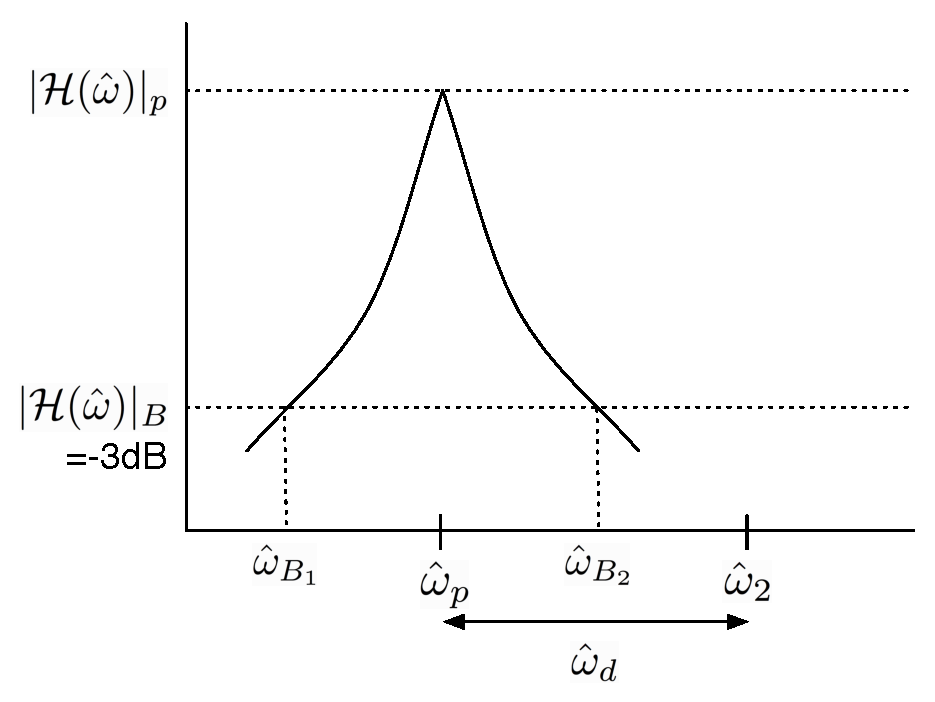
\includegraphics[height=3.5in]{ch-iir/design-example}}
\caption[Feedback filter design]{Designing a simple one-pole feedback
  filter. A filter's frequency 
  response is sketched for the situation where we want the center of
  its passband at $\hat{\omega}_p$ and we wish to ensure that another
  frequency, $\hat{\omega}_2 = \hat{\omega}_p + \hat{\omega}_d$, is
  well outside the passband. We choose 
  the filter's cutoff frequencies, $\hat{\omega}_{B_1} =
  \hat{\omega}_p - \hat{\omega}_B$ and $\hat{\omega}_{B_2} =
  \hat{\omega}_p  + \hat{\omega}_B$, to achieve this.
  \label{fig:design-example}}
\end{figure}

Let's consider how we might use these observations to design a filter,
as sketched in figure~\ref{fig:design-example}. We want the peak of the
filter's frequency response (the center of its passband) to be at the
frequency $\hat{\omega}_p$ and we want to ensure that it filters out
some other frequency, $\hat{\omega}_2$. We choose the -3dB points to
be at a distance $\pm\hat{\omega}_B$ from $\hat{\omega}_p$, labelled
$\hat{\omega}_{B_1}$ and $\hat{\omega}_{B_2}$ in the figure. These
cutoff frequencies are chosen to ensure that $\hat{\omega}_2$ is well
outside the passband.

Our design problem is to choose the pole location. The peak frequency
for the passband, $\hat{\omega}_p$, gives us the pole angle, so all we
need to do is determine the pole radius, $R$, to give us
$a_1=Re^{j\hat{\omega}_p}$. Looking at equation~(\ref{eq:reson-mag}),
we can substitute this value of $a_1$ and $z=e^{j\hat{\omega}}$ and
collect terms:
\begin{align}
|\mathcal{H}(\hat{\omega})| &=
\left|\frac{1}{1-Re^{j\hat{\omega}_p}e^{-j\hat{\omega}}}\right| \notag\\
  &= \left|\frac{1}{1-Re^{j(\hat{\omega}_p - \hat{\omega})}}\right|
\end{align}
We just need to make sure that when the frequency $\hat{\omega} =
\hat{\omega}_2$, $|\mathcal{H}(\hat{\omega})|$ is below -3dB. Clearly,
we can achieve this by ensuring that the half bandwidth, $B$, is less
than $\hat{\omega}_d$. We can then use equation~(\ref{eq:calc-bw}) to
determine the value of $R$ that ensures this, and we have the correct
pole location.

\problemset{
\subsubsection{Self-Test Exercises}

See~\ref{sc:ch4ex} \#\ref{it:ch4ex1}--\ref{it:ch4ex2} for answers.

\begin{enumerate}
\item Derive equation~(\ref{eq:fb-band2b})
  from~(\ref{eq:fb-band2a}).
\item In the situation where the sampling rate is 44,100Hz and the
  desired bandwidth is 20Hz, $R$ in~(\ref{eq:calc-bw}) is 0.998575.
  Solve for $R$ the situation where the desired bandwidth is 200Hz. Is
  it true that when $R$ is far away from one, $B$ grows large?
\end{enumerate}}

\section{Mixing Feedback and Feedforward Filters}

We have now seen feedforward filters with zeros in the transfer
function and feedback filters with poles. Zeros suppress frequency
components and poles enhance them.  Quite often, we want to combine
poles and zeros to improve the filter's features, such as the flatness
of the passband and the abruptness with which its response transitions
between the passband and the stop band.  Generally, the transfer
function of a filter with block diagram in
figure~\ref{fig:fb-nterm-bdiag} can written as
\begin{equation}
H(z)=\frac{b_0+b_1z^{-1}+\cdots+b_Mz^{-M}}{1+a_1z^{-1}+\cdots+a_Nz^{-N}}
\label{eq:gen-xfer}
\end{equation}
and the filter is  
\begin{equation}
y[n] = \underbrace{b_0x[n] + b_1x[n-1] + \cdots +
      b_Mx[n-M]}_{\text{feedforward terms}}
      - 
      \underbrace{a_1y[n-1] - \cdots - a_ny[n-N]}_{\text{feedback terms}}
\label{eq:gen-impl}
\end{equation}

\afterpage{
\begin{figure}
\centerline{\begin{tabular}{cc}
\noindent\parbox[c]{0.45\textwidth}{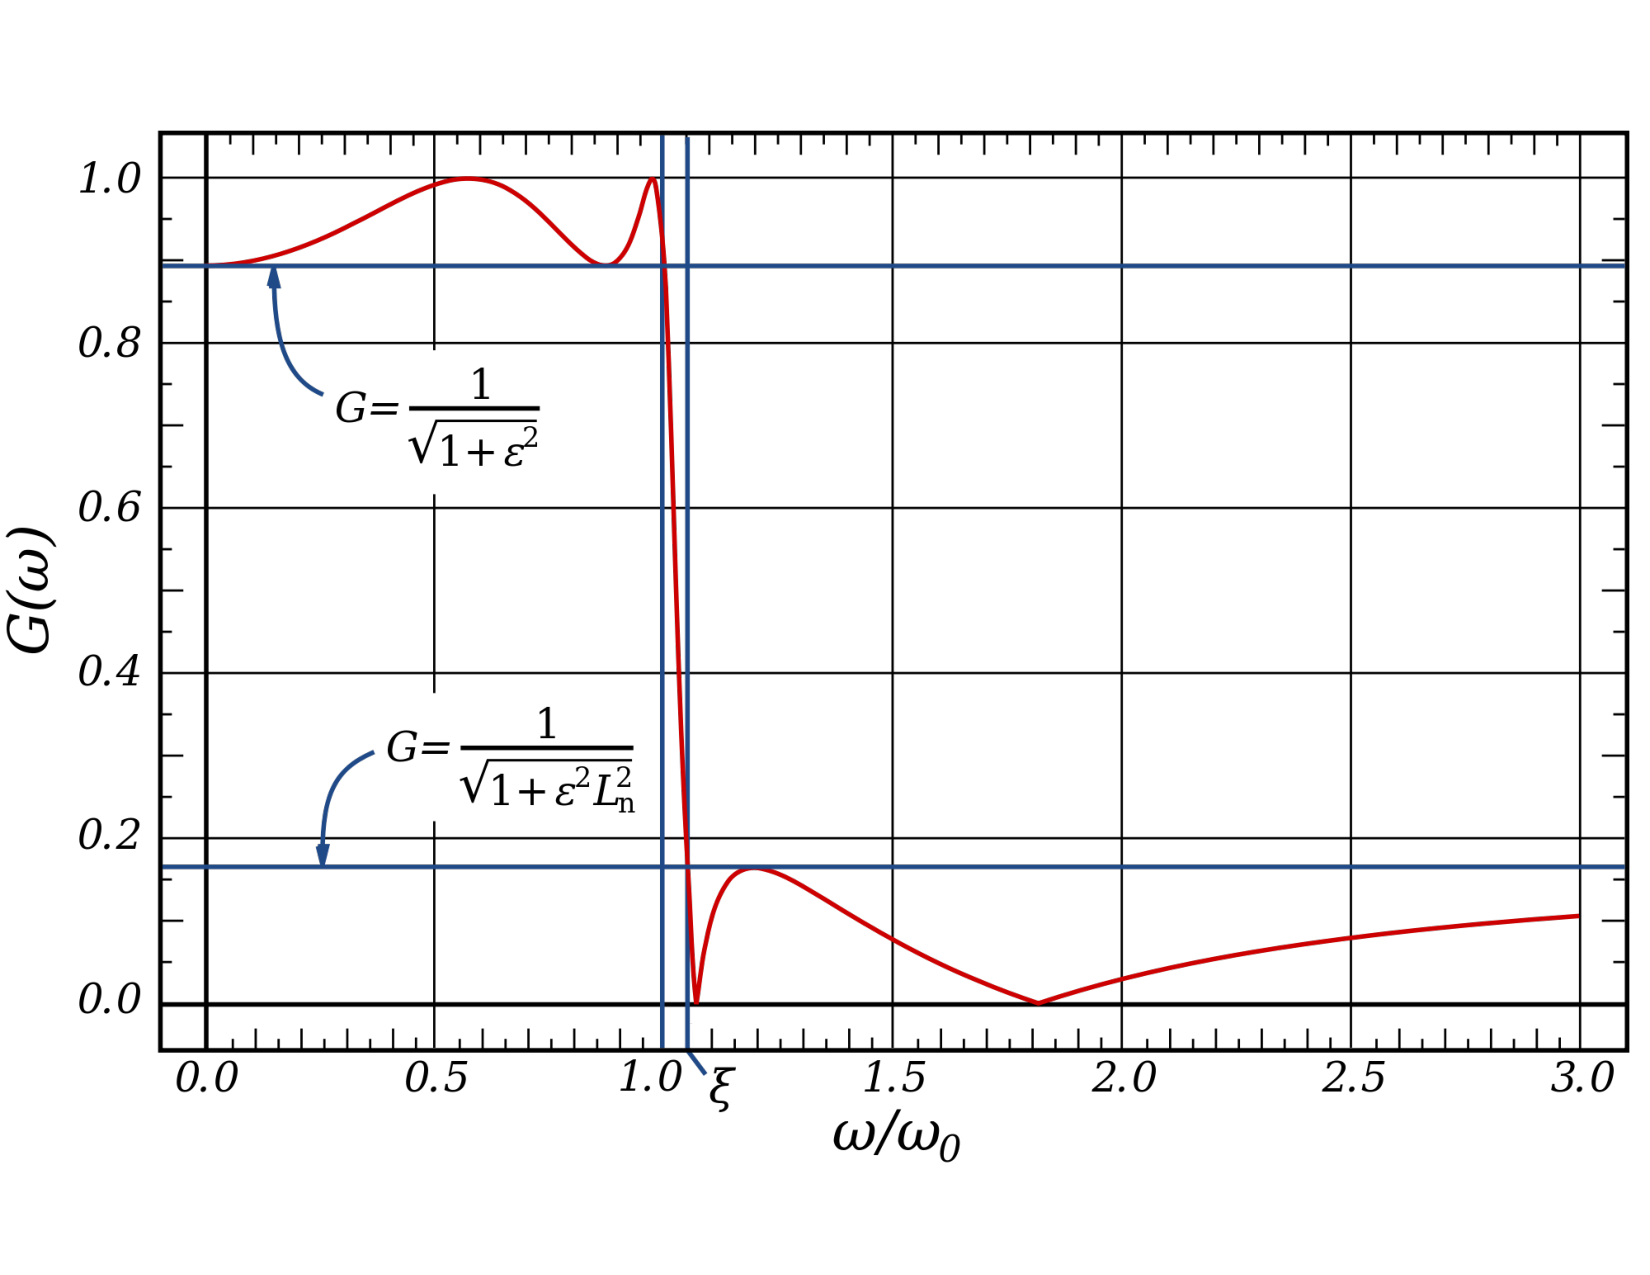
\includegraphics[width=0.45\textwidth]{ch-iir/Elliptic-Filter-Response}}
  &
\noindent\parbox[c]{0.45\textwidth}{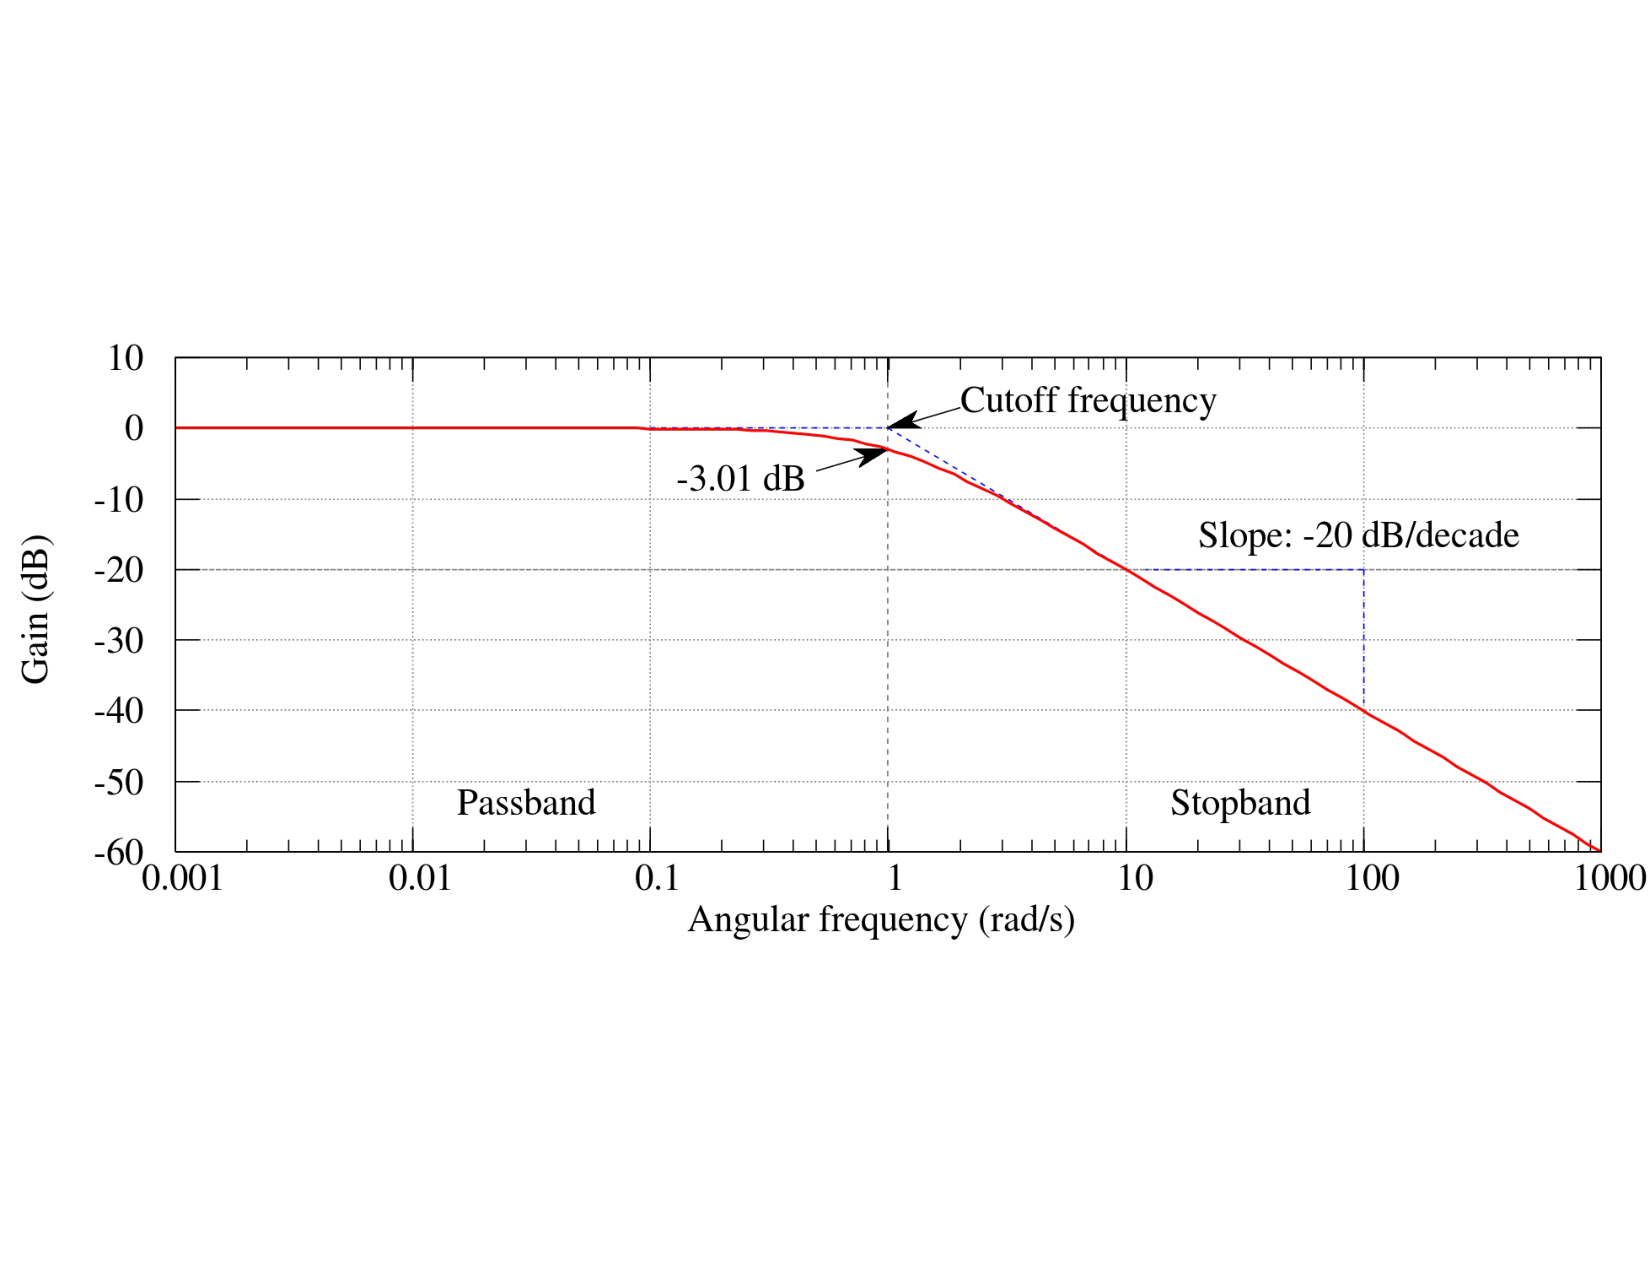
\includegraphics[width=0.45\textwidth]{ch-iir/Butterworth-Filter-Response}}
\end{tabular}}
\caption[Example filter frequency responses]{Example filter frequency
  responses: elliptic (left)\protect\footnotemark and Butterworth
  (right)\protect\footnotemark.\label{fig:filter-fr-examples}}
\end{figure}
\addtocounter{footnote}{-1}
\footnotetext{By Inductiveload (Own work) [Public domain], via
    Wikimedia Commons.}
\footnotetext{By Alejo2083 (Own work) [GFDL
  (\url{http://www.gnu.org/copyleft/fdl.html)}, CC-BY-SA-3.0
  (\url{http://creativecommons.org/licenses/by-sa/3.0/}) or CC BY-SA
  2.5-2.0-1.0
  (\url{http://creativecommons.org/licenses/by-sa/2.5-2.0-1.0})], via
  Wikimedia Commons.}
}

Depending on the coefficients $\{b_k\}$ and $\{a_\ell\}$, the
filter will show different features. Some of these features have
proven so useful that these forms of~(\ref{eq:gen-xfer}) have acquired
special names, such as elliptic, Butterworth, etc. (usually, based on
the form of the numerator and/or denominator
polynomial). Figure~\ref{fig:filter-fr-examples} presents some example
frequency responses.

\section{Implementation}

Just as in chapter~\ref{ch:filt-intro}, feedback filters have their
delays implemented with queues which are ``circular arrays''.
However, there are two additional complications that we must deal
with: complex poles and accuracy of numerical computation.

\subsection{Avoiding Complex Numbers}

In principle, there is no reason that we couldn't perform all our
computations using complex numbers and just output the real part of
the result as the filtered signal.  However, we often want to perform
filtering in real time, and so would like to avoid any unnecessary
computation. A cute trick allows us to eliminate the need for complex
numbers.

\emph{Remember that all complex poles will appear in conjugate pairs.}
Since each pole is a root of a polynomial, that means that the
denominator of the filter's transfer function will have even degree
(excepting the real-valued poles, of course), and when it is factored
the conjugate pairs $(z_i,z_i^*)$ will appear as $(z-z_i)(z-z_i^*)$.
If we multiply this out, we get $z^2 - 2\Real[z_i] z +|z_i|^2$. In
other words, the imaginary parts of poles cancel each other out.
Since we're already using $b_k$ for the feedforward coefficients and
$a_\ell$ for the feedback ones in the filter equation, let's set $c_i
= -2\Real[z_i]$ and $d_i = |z_i|^2$.  If the transfer function's
denominator is of order $N$ ($N$ even), then we can multiply out the
polynomials for each complex conjugate pair and rewrite the
denominator as the product of $N/2$ second-order polynomials
\begin{equation}
(z^2+c_0z+d_0)(z^2+c_1z+d_1)\cdots (z^2+c_{N/2-1}z+d_{N/2-1})
\end{equation}
with no need for complex arithmetic.  We've done this before
symbolically, using Euler's formula to eliminate the imaginary part of
a complex conjugate pair. The point here is that, since complex poles
always appear in conjugate pairs, we can do this with even quite
complicated filters to eliminate the need for performing complex
arithmetic or processing complex numbers --- a significant
optimization.

\subsection{Limitations of Numerical Accuracy}

When we talk of the mathematics of filters, we assume that numbers
have infinite precision.  Unfortunately, this is not the case for
computer implementation.  These days, computers (including digital
signal processors) typically use either 32 or 64 bits to represent
numbers (be they fixed or floating point).  That may seem like a great
deal of precision, but it is unfortunately not uncommon for
intermediate results in numerical computation to require many more
bits to retain needed precision.  There are a number of ways this can
happen, but one is where a computation is performed iteratively, so
that a long chain of operations is applied to inputs before they
become outputs. At each step of this chain, the result has limited
precision. In other words, the number we get is not exactly correct
--- in general, it can't be, since we don't have infinite precision.

This loss of precision can mount rapidly, eventually destroying the
result. We can think of this limited precision as an \emph{error}. If
the input is from a 16-bit A/D, for example, and we assume it does its
conversion absolutely accurately to the smallest bit (which, as you
have seen in chapter~\ref{ch:computer-signals} and will revisit in
chapter~\ref{ch:compression}, is probably not realistic), then that's
around $\log_{10} 2^{16} \approx 5$ decimal digits from the A/D, to be
generous. Each arithmetic operation we perform, regardless of the
number of bits we use, can have the undesirable effect of decreasing
the number of digits of precision we have.  Sums of approximate values
have errors which are the sums of their addends' errors.
Multiplication tends to magnify errors. Let's see this with a simple
example.

\paragraph{Example~4}
Consider the following two recurrence relations for computing the
\index{recurrence relation}
series $\{x[n]\} = \{1/3^n\}$ ($n = 0, 1, 2, \ldots$):
\begin{align}
x'[n]  &= \frac{1}{3} x'[n-1] \label{eq:series-direct} \\
x''[n] &= \frac{10}{3} x''[n-1] - x''[n-2]
\label{eq:series-twoterms}
\end{align}
Both of these equations are mathematically ``correct''. \emph{They
also look like the expressions we use for our filters.}  Yet, they
yield very different results because of loss of significance.  Let's
use an initial value of $x'[0] = 0.99996$ for~(\ref{eq:series-direct})
and initial values of $x''[0]=1$ and $x''[1]=0.33332$
for~(\ref{eq:series-twoterms}). This is an initial error of 0.00004
for $x'[0]$ and $0.00001\bar{3}$ for $x''[1]$. I'll use MATLAB to
compute the first ten terms in each sequence with double-precision
accuracy for each calculation.  The MATLAB code is
\index{MATLAB code!numerical error|(}

\begin{small}
\begin{verbatim}
% significance.m
% 2/22/02 MDS
% Examine how error grows in an iterative computation
stdout = 1;

% This isn't efficient, but it is straightforward

% Values of n for computation
n = [0:10];

% Series 1: the real McCoy
x = 1./3.^n;

% Series 2: x'[n] = 1/3 x'[n-1]
xp = 0.99996;

for n = [1:10],
  xp(n+1) = 1/3 * xp(n);  % Remember, MATLAB indices start at 1, not 0
end;

% Series 3: x''[n] = 10/3 x''[n-1] - x''[n-2]
xpp = [1 0.33332];

for n = [2:10],
  xpp(n+1) = 10/3 * xpp(n) - xpp(n-1);
end;

% Print out the results
fprintf(stdout, ' n          x[n]            x''[n]           x''''[n]\n');
for n = [0:10],
  fprintf(stdout, '%2.1d\t%12.10f\t%12.10f\t%12.10f\n', ...
          n, x(n+1), xp(n+1), xpp(n+1));
end;
\end{verbatim}
\end{small}

The output this script produces is:
\begin{verbatim}
 n          x[n]            x'[n]           x''[n]
 0      1.0000000000    0.9999600000    1.0000000000
 1      0.3333333333    0.3333200000    0.3333200000
 2      0.1111111111    0.1111066667    0.1110666667
 3      0.0370370370    0.0370355556    0.0369022222
 4      0.0123456790    0.0123451852    0.0119407407
 5      0.0041152263    0.0041150617    0.0029002469
 6      0.0013717421    0.0013716872    -0.0022732510
 7      0.0004572474    0.0004572291    -0.0104777503
 8      0.0001524158    0.0001524097    -0.0326525834
 9      0.0000508053    0.0000508032    -0.0983641945
10      0.0000169351    0.0000169344    -0.2952280648
\end{verbatim}
\index{MATLAB code!numerical error|)}

The first column is accurate to the full precision of IEEE floating
point (that is, the computation is that accurate; the output was
limited to ten decimal places).  The second column's error is
\emph{stable}: it decreases in an exponential manner, and the value
for $x'[10]$ is within $7 \times 10^{-10}$ of the actual value. The
third column's error is \emph{unstable}: it increases exponentially.

Couple this with the need for precise pole placement, and you
can see that we need to be careful about our implementations. We saw
in this chapter's section on combining feedforward and feedback
filters the general transfer function for a filter~(\ref{eq:gen-xfer})
and its direct implementation~(\ref{eq:gen-impl}), which involved
$M$ delayed values of $x$ and $N$ delayed values of $y$.

\index{filter!cascade}
However, it is better to implement such a digital filter as a cascade
of second-order ones, by factoring the numerator and denominator
(which should be ``easy,'' since we know the locations of the poles
and zeros) and multiplying out terms with complex conjugate pairs as
described in the previous section. The resultant fraction will have
numerator and denominator which are each a product of second-order
polynomials.  Each ratio of second-order polynomials is a subfilter,
which can be implemented by a simple update equation. If we take the
output of one subfilter and present it as the input of the next, the
output of the last subfilter will be equivalent to the output of the
entire original filter (we saw this cascade of filters in
chapter~\ref{ch:filt-intro}). Note that, though each filter has a very
short (two step) queue, the series combination produces what amounts
to a longer overall queue. In practical applications, this shouldn't
be much of a computational penalty.

\section{Problems}


\section{Further Reading}

\begin{itemize}
\item James H McClellan, Ronald W. Schafer, and Mark A. Yoder,
  \textit{DSP First: A Multimedia Approach}, Prentice Hall, 1998,
  chapter 8 (\S 8.1--8.6, 8.8).
\end{itemize}


% LocalWords:  feedforward phasor reson

% \include{chapter5/fourier}  % Superseded by ch-fft/fft
% -*-LaTeX-*-

% $Log: fft.tex,v $
% Revision 1.9  2010/03/16 00:22:18  stiber
% Correction of minor error in equation (6-56).
%
% Revision 1.8  2007/12/25 19:02:53  stiber
% Minor fixes.
%
% Revision 1.7  2007/12/16 23:34:56  stiber
% Modifications for Winter 2008. This was somewhat extensive, actually,
% including a worked example 8-point FFT.
%
% Revision 1.6  2007/03/20 23:54:19  stiber
% Updated eqnarray to align.
%
% Revision 1.5  2007/03/20 22:26:56  stiber
% Modified to make into stand-alone textbook, plus numerous improvements
% and LaTeX updating.
%
% Revision 1.4  2006/05/13 17:09:35  stiber
% Fixed problems with figure fft_sin_xX. Figure right after it had a
% name fft_sin_XX, and there was a problem with case insensitivity
% in MATLAB which caused the second figure to be the same as the first.
% Regenerated both figures in MATLAB, named the second fft-leakage.
%
% Revision 1.3  2006/03/27 23:39:10  stiber
% Fixed small error (Hamming vs. Hann).
%
% Revision 1.2  2004/03/29 19:52:39  stiber
% Updated for Spring 2004 and new textbook (DSP First).
%
% Revision 1.1  2004/02/19 00:26:42  stiber
% Initial revision
%

\chapter{Spectral Analysis}
\label{ch:fft}

We begin our study of signal frequency analysis with the
representation of continuous-time periodic and aperiodic signals by
means of the \emph{Fourier Transform}.  This is followed by a
treatment of discrete-time signals, that is the
\emph{Discrete Fourier Transform} and an efficient algorithm for
computing it: the \emph{Fast Fourier Transform} (FFT). After this
chapter, you should understand what they are and how the FFT works. You
should also understand related terms, for example, \emph{fundamental
frequency}, \emph{harmonics}, \emph{spectrum}, \emph{time domain}, and
\emph{frequency domain}. You should be able to use them to do some
frequency analysis of a signal.  We will also go over some problems
that you need to keep in mind when using them:
\emph{power leakage} caused by sudden changes in the signal, the
\emph{tradeoff between time and frequency resolution}, and the
function of
\emph{windows}. You should be able to use this knowledge to guide what
you do to obtain accurate results in estimating spectral information.

\section{The Fourier Transform}
\label{sc:fourier-xform}

\index{Fourier Transform|emph}
We developed the Fourier series to represent a \emph{periodic} signal
as a linear combination of harmonically related complex
exponentials:
\begin{equation}
  x(t) = \sum_{k=-\infty}^{+\infty} c_k e^{j2\pi k f_0t}
\end{equation}
Here, the $c_k$ are the Fourier coefficients and the sequence $\ldots,
c_{-1}, c_0, c_1, \ldots$ can be thought of as the frequency domain
representation (the amplitudes of the complex sinusoids) of the time
domain signal $x(t)$.  For continuous time \emph{aperiodic} signals
$x(t)$, the Fourier Transform is defined. It can be derived from the
Fourier series allowing the signal period $T$ to go to infinity.  Here
I'll just give its definition:
\begin{align}
x(t) &= \int_{-\infty}^{\infty}X(f)e^{j2\pi ft}df
\label{eq:ft-x} \\
X(f) &= \int_{-\infty}^{\infty}x(t)e^{-j2\pi ft}dt
\label{eq:ft-X}
\end{align}

Equation~(\ref{eq:ft-X}) is the \emph{Fourier transform} of $x(t)$: a
function of the continuous frequency variable
$f$. Equation~(\ref{eq:ft-x}) is called the \emph{inverse Fourier
  transform}, which yields $x(t)$ when $X(f)$ is known. The Fourier
transform converts an infinite-duration (aperiodic), continuous signal
in the time domain into an infinite, continuous spectrum in the
frequency domain. It is apparent that the essential difference between
the Fourier series and the Fourier transform is that the spectrum in
the latter is continuous (the Fourier series yields a discrete line
spectrum; it has non-zero values only at specific frequencies) and
hence the synthesis of an aperiodic signal from its spectrum is
accomplished by means of integration instead of summation. The Fourier
transform pair in~(\ref{eq:ft-X}) and~(\ref{eq:ft-x}) can also be
expressed in terms of the radian frequency variable $\omega = 2\pi
f$. Since $f = \omega/(2\pi)$, the pair becomes
\begin{align}
x(t) &= \int_{-\infty}^{\infty}X(\omega)e^{j\omega t}d\omega\\
X(\omega) &= \int_{-\infty}^{\infty}x(t)e^{-j\omega t}dt
\end{align}

\subsection{Example: Fourier transform of a rectangular pulse}

\begin{figure}
\centerline{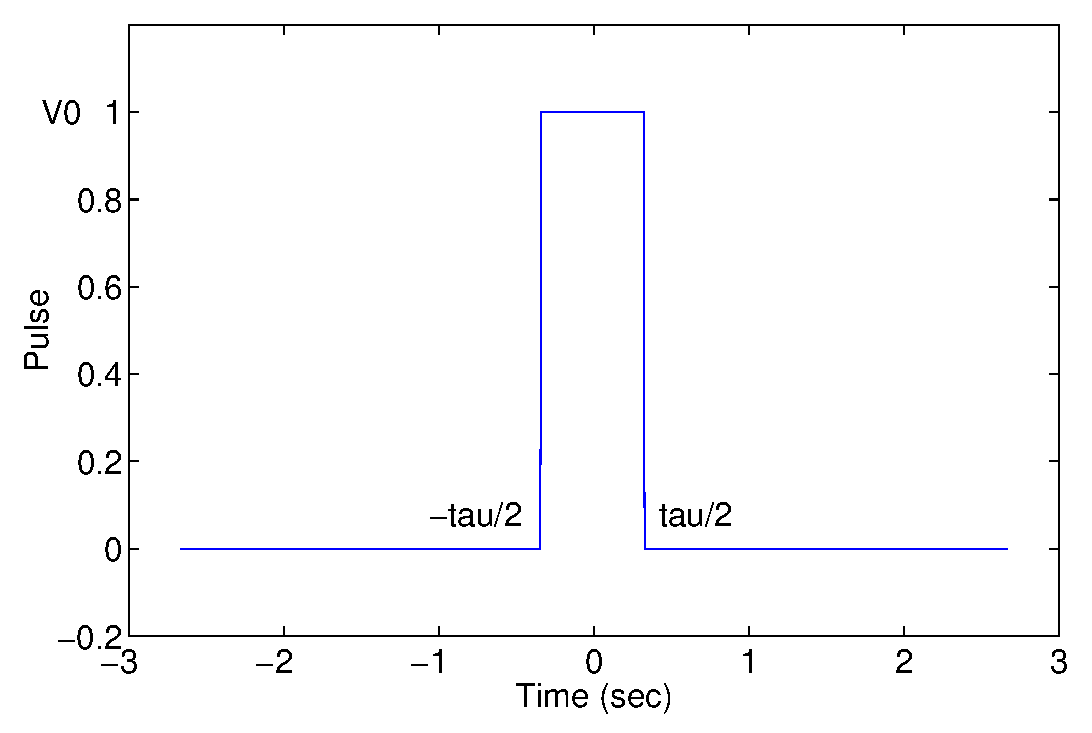
\includegraphics[height=3in]{ch-fft/ft_pulse}}
\caption{A rectangular pulse with width $\tau$. 
\label{fig:ft-pulse-x}}
\end{figure}

Let's look at the rectangular pulse written about before; but here
the pulse is aperiodic --- there is just a single pulse instead of a
train of them. The signal is defined as
\begin{equation}
x(t) = \left\{\begin{array}{ll}
                        1 & |t|\leq \tau/2 \\
                        0   & |t| > \tau/2
                        \end{array}\right.
\end{equation}
and illustrated in Figure~\ref{fig:ft-pulse-x}.  

\begin{figure}
\centerline{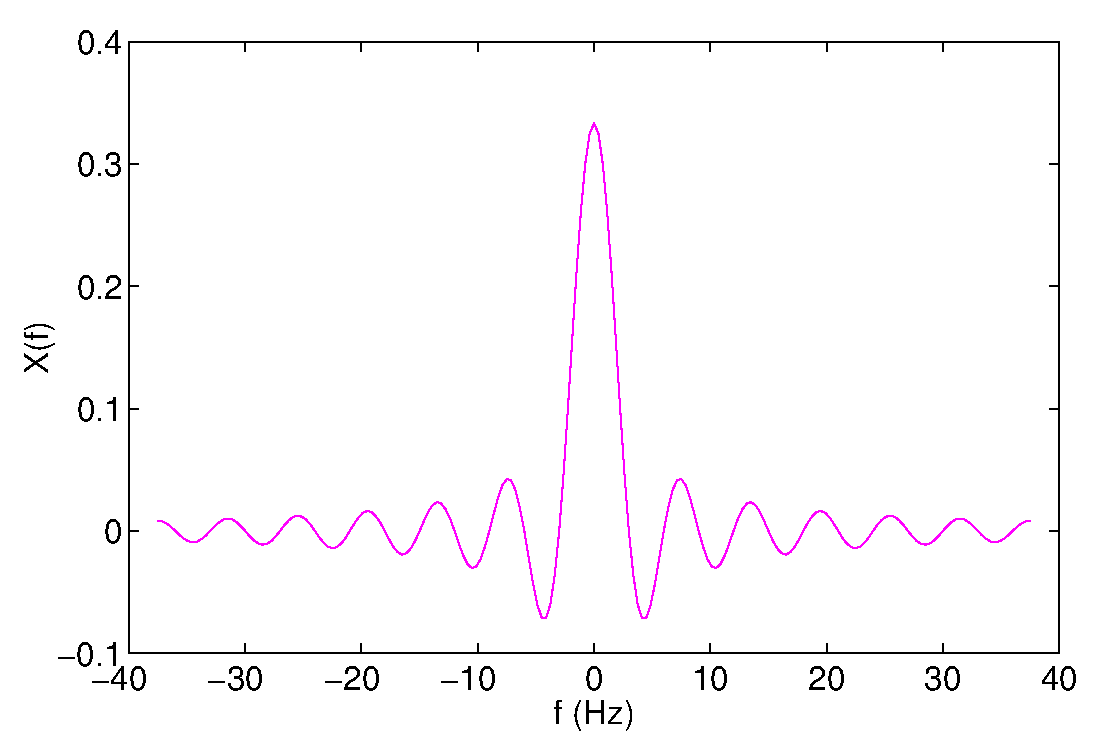
\includegraphics[height=3in]{ch-fft/ft_pulseX}}
\caption{Fourier transform of the pulse in
figure~\protect\ref{fig:ft-pulse-x}.
\label{fig:ft-pulse-X}}
\end{figure}

\index{Fourier Transform!of a pulse}
By applying~(\ref{eq:ft-X}), we find that
\begin{align}
X(f) &= \int_{-\tau/2}^{+\tau/2} e^{-j2\pi ft}dt \notag\\ 
     &= \left.\frac{e^{-j2\pi ft}}
                      {-j2\pi f}\right|_{-\tau/2}^{+\tau/2} \notag\\ 
     &= \frac{1}{-j2\pi f}[e^{-j\pi f\tau}-e^{j\pi f\tau}] \notag\\
     &= \tau\sinc(\pi f \tau)
\label{eq:ft-pulse-X}
\end{align}
The final step in deriving~(\ref{eq:ft-pulse-X}) made use of the
observation that the difference of a complex number and its conjugate
is just twice its imaginary part, $(a-jb) - (a+jb) = -2jb$. In polar
notation, then, $e^{-j\pi f \tau} - e^{j\pi f \tau} = -2j\sin\pi f
\tau$, using Euler's formula. We observe that $X(f)$ is real and has
the shape of the sinc function we mentioned previously. The important
difference here is that it is a \emph{continuous} spectrum instead of
line spectrum.  It is shown in figure~\ref{fig:ft-pulse-X}.

\begin{figure}
\centerline{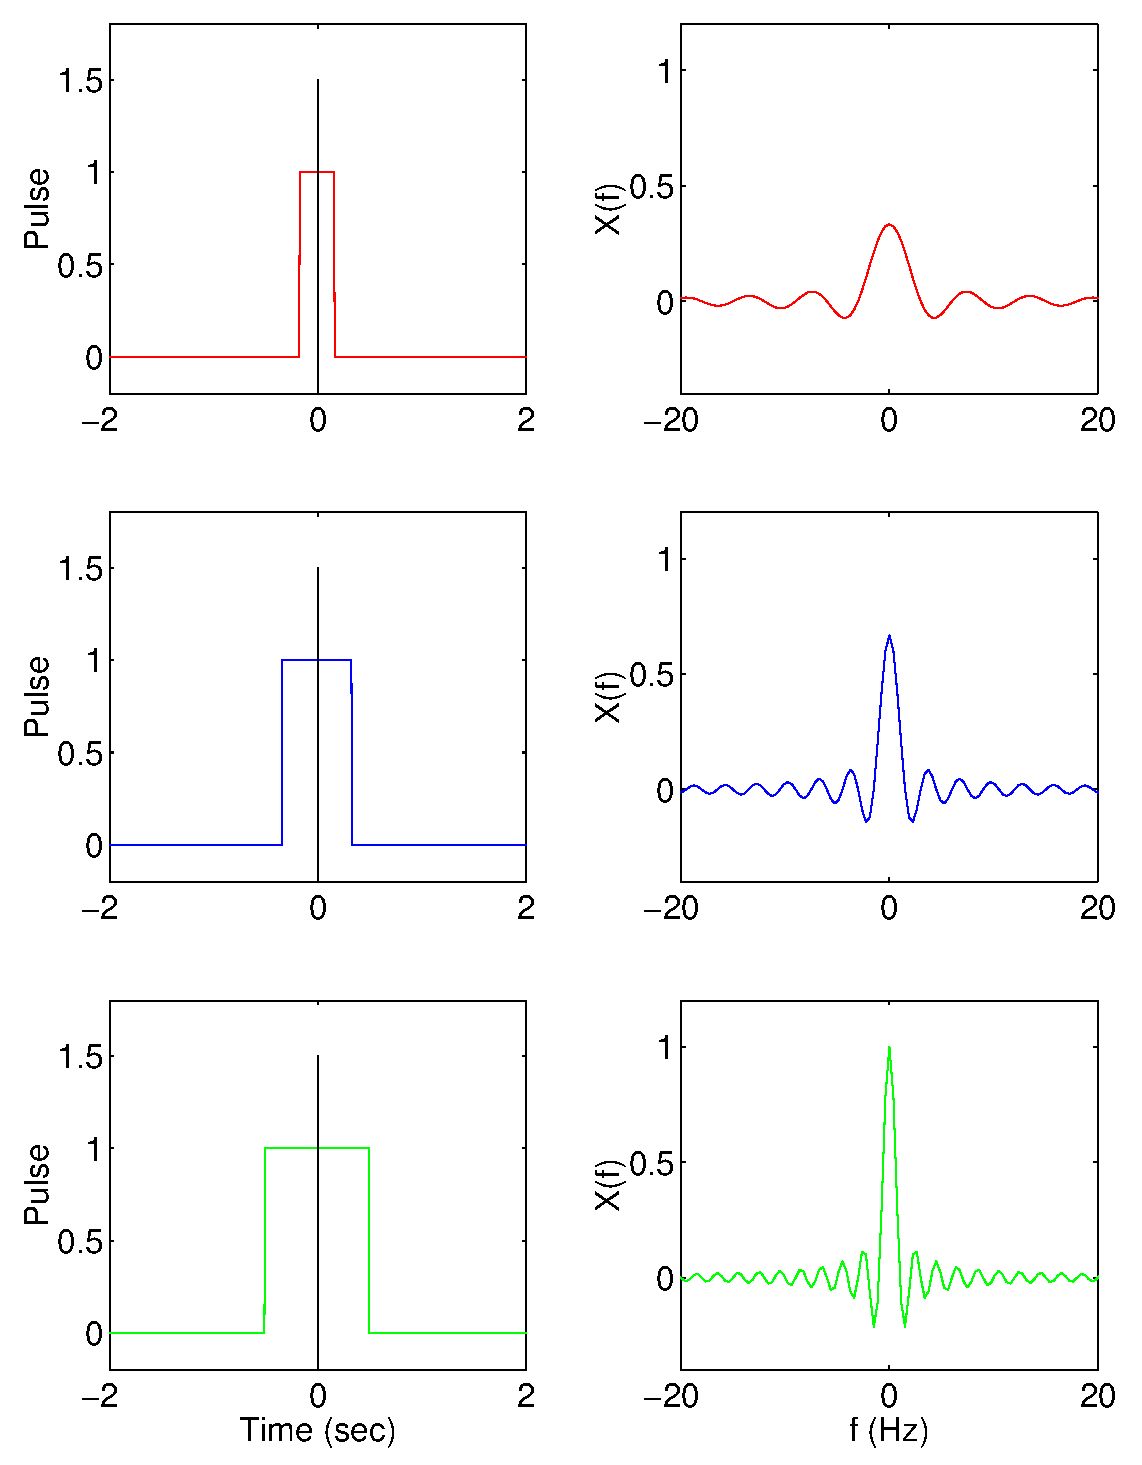
\includegraphics[width=5in]{ch-fft/ft_pulse_xX}}
\caption[Fourier transform of a rectangular pulse for various width 
values]{Fourier transform of a rectangular pulse for various width
values $\tau$.\label{fig:ft-pulse-xX}}
\end{figure}

As with the periodic rectangular pulses, from~(\ref{eq:ft-pulse-X}) we
note that the zero crossings of $X(f)$ occur at multiples of $1/\tau$.
Furthermore, the width of the main lobe, which contains most of the
signal energy, is equal to $1/\tau$. As the pulse duration $\tau$
decreases or increases, the main lobe becomes broader or narrower, and
more energy is moved to the higher or lower frequencies, respectively,
as is illustrated in figure~\ref{fig:ft-pulse-xX}. Thus, as the single
pulse is expanded (compressed) in time, its transform is compressed
(expanded) in frequency.

\section{The Discrete Fourier Transform}

So far, we have examined the Fourier series (which is for a
periodic, continuous signal) and its discrete spectrum and the Fourier
transform (which is for an aperiodic, continuous signal) and its
continuous spectrum. Now, we will investigate periodic, \emph{discrete}
signals and their spectra, which are discrete.

Let's consider a finite digital signal $\{x[n]\}$ ($n=0,1,2,\ldots,
N-1$). The discrete Fourier transform (\emph{DFT}) is defined as
\index{Discrete Fourier Transform (DFT)}
\begin{equation}
X[k] = \sum_{n=0}^{N-1} x[n] e^{-j n k 2\pi/N}, \quad k = 0,1,2,\ldots,
N-1
\label{eq:dft}
\end{equation}
where $X$ is the spectrum of $x$, and its synthesis equation or
inverse DFT (\emph{IDFT}) is
\begin{equation}
x[n]=\frac{1}{N} \sum_{k=0}^{N-1} X[k] e^{j n k 2\pi/N}, \quad
n=0,1,2,\ldots, N-1
\label{eq:idft}
\end{equation}

The DFT converts a finite (periodic), discrete signal in
the time domain ($x[n]$) into a finite, discrete spectrum in the frequency
domain ($X[k]$).

We can derive the DFT informally from the Fourier series of a periodic
signal. Let's compare equation~(\ref{eq:dft}) and that for the
coefficients of the Fourier series, equation~(\ref{eq:fs-ck}), which I
repeat here:
\begin{equation}
c_k=\langle f(t), e^{jk\omega_0 t}\rangle = \frac{1}{T}\int_0^T f(t)e^{-jk\omega_0
t}dt
\label{eq:fs-ckrepeat}
\end{equation}

First, notice that the DFT uses a summation within $[0, N-1]$ and the
series uses an integral within one period T.  This difference arises
because here the signal is discrete and finite (and so we write $x[n]$
instead of $f(t)$). The factor of $1/T$ in~(\ref{eq:fs-ckrepeat}) is
equivalent to that of $1/N$ in~(\ref{eq:idft}), where 
that factor has been arbitrarily included in the IDFT instead of the DFT.

Now let's compare the basis (the complex exponential). The frequency
here is also discretized.  Remember that a sampled signal has a
Nyquist frequency of $\omega_s/2$, or $\pi$ radians/sample, where
$\omega_s$ is the sampling rate, equivalent to $2\pi$ radians/sample.
Let's discretize this signal's frequencies using $N$ equally-spaced
points.  The step $\Delta\hat{\omega}$ between neighboring frequencies (in
radians/sample) is
\begin{equation}
\Delta\hat{\omega} = \frac{2\pi}{N}
\end{equation}
This is what equation~(\ref{eq:dft}) indicates within the sum: that
whatever $nk$ is, it will be a multiple of $2\pi/N$.  The
$k^\mathrm{th}$ frequency in radians can be written as
\begin{equation}
k \Delta\hat{\omega} = k\frac{2\pi}{N}, \quad k = 0, 1, 2, \ldots, N-1
\label{eq:dft-w}
\end{equation}

Substituting $k \Delta\hat{\omega}$ in~(\ref{eq:dft-w}) for
$k\omega_0$ in the Fourier series basis should convince you that the
DFT is the discrete version of the Fourier series. The coefficient
$X[k]$ is the magnitude of the spectrum of $x$ at frequency $k2\pi/N$.

\begin{table}
  \centering
  \begin{tabular}{|l|l|l|l|l|l|} \hline
    $T$ (s) & $f_s$ (Hz) & $N$ & $\Delta\hat{\omega}$ (rad/sample) &
    $\Delta\omega$ (rad/s) & $\Delta f$ (Hz) \\ \hline
    1    & 10    & 10    & $\pi/5$    & $2\pi$    & 1 \\
    10   & 10    & 100   & $\pi/50$   & $\pi/5$   & $1/10$ \\
    100  & 10    & 1000  & $\pi/500$  & $\pi/50$  & $1/100$ \\
    100  & 5     & 500   & $\pi/250$  & $\pi/50$  & $1/100$ \\
    100  & 1     & 100   & $\pi/50$   & $\pi/50$  & $1/100$ \\ \hline
  \end{tabular}
  \caption{Some examples of how $\Delta\hat{\omega}$,
    $\Delta\omega=\Delta\hat{\omega}f_s$, 
    and $\Delta f=\Delta\omega/2\pi = f_s/N$ change for signals of
    different duration and sampling rate.} 
  \label{tb:delta-f}
\end{table}

Table~\ref{tb:delta-f} illustrates how the step between frequencies
changes as the signal duration and sampling rate (and thus number of
samples) change. Increasing the signal duration, and therefore the
number of samples, without changing the sampling rate (which keeps the
Nyquist cutoff constant) decreases the step between frequencies (or,
if you prefer to think of this another way, increases the frequency
resolution). On the other hand, decreasing the sampling rate decreases
the number of samples (assuming the signal duration stays constant)
and the Nyquist cutoff, so the step between frequencies stays
constant.

\subsection{Derivation of the IDFT [\textsc{Optional}]}

Next, let's see how we can get the synthesis equation IDFT from the
DFT. Multiplying both sides of~(\ref{eq:dft}) by $e^{j n' k 2\pi/N}$
and then summing over all $k$,
\begin{equation}
\sum_{k=0}^{N-1} X[k] e^{j n' k 2\pi/N} 
= \sum_{k=0}^{N-1}\sum_{n=0}^{N-1} x[n] e^{-j n k 2\pi/N}e^{j n' k
2\pi/N} 
\end{equation}
Switching the order of summation of $n$ and $k$ on the right side,
plus some algebraic rearrangement yields
\begin{equation}
\sum_{k=0}^{N-1} X[k] e^{j n' k 2\pi/N}
= \sum_{n=0}^{N-1} x[n] \sum_{k=0}^{N-1} e^{j k(n'-n)
2\pi/N}
\label{eq:dft-2idft1}
\end{equation}
It can be shown that
\begin{align}
\sum_{k=0}^{N-1} e^{j k(n'-n)2\pi/N} 
&= \left\{\begin{array}{ll}
                        N & n=n' \\
                        0 & n \neq n'
           \end{array}\right.\\
&= N\delta[n-n']
\end{align}
where $\delta[n-n']$ is defined as
\begin{equation}
\delta[n-n'] = \left\{\begin{array}{ll}
                        1 & n=n' \\
                        0 & n \neq n'
                      \end{array}\right.
\end{equation}

Substituting the above result into~(\ref{eq:dft-2idft1}), we get the
IDFT (but for that pesky factor of $1/N$):
\begin{align}
\sum_{k=0}^{N-1}X[k] e^{j n' k 2\pi/N}
  &= \sum_{n=0}^{N-1}x[n] N\delta[n-n'] \notag\\
  &= Nx[n']
\end{align}

To simplify the notation, let's use a vector notation for the
discrete signal $\mathbf{x}=\{x[n]\}$ and its spectrum
$\mathbf{X}=\{X[k]\}$.  The DFT and IDFT operations become $N\times N$
matrices $\mathbf{F}$ and $\mathbf{F^{-1}}$, respectively. An element
in row $k$ and column $n$ of $\mathbf{F}$ is
\begin{equation}
[\mathbf{F}]_{kn}= e^{-jnk2\pi/N}, \quad k,n=0,1,2,\ldots,N-1
\end{equation}
Then the DFT and IDFT can be written as
\begin{align}
\mathbf{X} &= \mathbf{F}\mathbf{x}\\
\mathbf{x} &= \mathbf{F^{-1}}\mathbf{X}
\end{align}
or 
\begin{gather}
\mathbf{x}\stackrel{\mathbf{F}}{\longrightarrow} \mathbf{X}\\
\mathbf{X}\stackrel{\mathbf{F^{-1}}}{\longrightarrow} \mathbf{x}
\end{gather}

\subsection{Finite vs. Infinite Signals}

In this book, we have used (and will continue to use) the terms
``periodic'' and ``finite'' interchangeably (and, similarly,
``aperiodic'' and ``infinite''). When we compute the Fourier series or
the DFT of a finite signal of duration $T$, we do so only within that
interval of time. In effect, what we are doing for finite signals is
``pretending'' that the signal is actually periodic with period $T$
and that we are only looking at one of its periods.

On the other hand, if a signal is actually of infinite duration, we
would use the Fourier transform. However, this is not a process that
we can perform on a computer, where infinite duration signals cannot
exist (the duration of any signal is limited by the available
storage). We have to chop the signal off at a length that the computer
can handle, ignoring the error it may produce (or testing to make sure
that the error is tolerable for our application). This brings us back
to the DFT for processing the resulting finite signal as an
\emph{approximation} of the infinite signal's Fourier transform. Note
that, even outside the computer, our time is finite (even the lifespan
of the universe is finite) and so no physically realizable signal is
actually infinite.


\subsection{Properties of the DFT}

\index{Discrete Fourier Transform (DFT)!properties of}
Let's consider some of the properties of the DFT of physically
realizable signals. These signals are real, so $x[n] = x[n]^*$. What
is the spectrum of such a signal like? We can think of the signal's
frequency content or spectrum, $X[k]$ ($k=0,1,\ldots,N-1$), as a
sequence of $N$ complex numbers. This is known as a \emph{$N$ point
FFT}. If we compute $X[N-k]$ using~(\ref{eq:dft}), we get
\index{FFT!points}
\begin{align*}
X[N-k] &= \sum_{n=0}^{N-1} x[n] e^{-j n (N-k) 2\pi/N} \\
&= \sum_{n=0}^{N-1} x[n] e^{-jn2\pi}e^{j n k 2\pi/N} \\
&= \sum_{n=0}^{N-1} x[n] e^{j n k 2\pi/N} &&\text{(since $e^{-jn2\pi}=1$)}\\
&= \left[\sum_{n=0}^{N-1} x[n]^* e^{-j n k 2\pi/N}\right]^* 
   &&\text{(since $ab = ((ab)^*)^* = (a^*b^*)^*$)}
\end{align*}
Because $x[n]=x[n]^*$,
\begin{align}
X[N-k]&= \left[\sum_{n=0}^{N-1} x[n] e^{-j n k 2\pi/N}\right]^* \notag\\
       &= X[k]^*
\end{align}

So for example, when $N=8$, $k=0, 1,2,3,4,5,6,7$, and
\begin{equation}
X[7]=X[1]^* \quad X[6]=X[2]^* \quad X[5]=X[3]^*
\end{equation}
(When $k=0$, $X[8]=X[0]^*$ but $X[8]$ is out of spectrum, which ranges
from 0 to 7 only. This is the ``DC'', or zero-frequency, component of
the signal.)

This can be represented diagrammatically as
\begin{equation}
\underset{\underset{\text{DC}}{\uparrow}}{0} \quad \underbrace{1 \quad
    \overbrace{2 \quad \underbrace{3 \quad 4 \quad 5} \quad 6} \quad 7}
\label{eq:dft8-freqs}
\end{equation}
This is clearly symmetric about $k=4$. When $N$ is an even number,
the spectrum has $N/2$ at the center; when $N$ is an odd number, the
center is between $\lfloor N/2 \rfloor$ and $\lceil N/2 \rceil$. So,
for $N=7$,
\begin{equation}
\underset{\underset{\text{DC}}{\uparrow}}{0} \quad \underbrace{1 \quad
  \overbrace{2 \quad \underbrace{3 \quad 4} \quad 5} \quad 6}
\end{equation}   

What this means is that the spectrum over frequencies $\lceil N/2
\rceil$ to $N-1$ has the same magnitude as over 1 to $\lfloor N/2
\rfloor$, but with negative phase angle (which means negative
frequencies on the unit circle). In fact, $N/2$ corresponds to the
Nyquist frequency in radians/sample. We can see this
from~(\ref{eq:dft-w}), when $k=N/2$
\begin{equation}
\hat{\omega}_{N/2}=\frac{N}{2}\frac{2\pi}{N}=\pi
\end{equation}
Converting this to Hz, we get
\begin{equation}
\hat{f}_{N/2} = \hat{\omega}_{N/2}\frac{f_s}{2\pi}
              = \pi\frac{f_s}{2\pi} = \frac{f_s}{2}
\end{equation}
where $f_s$ is the sampling rate. The above equation shows that
$\hat{f}_{N/2}$ is the Nyquist frequency in Hz. The conclusion is that
the magnitude of the transform of a real valued signal is an
\emph{even} function of frequency and so we only need to plot its
spectrum in range $[0, N/2]$, corresponding to the range of
frequencies from 0 to the Nyquist frequency. This also means that the
DFT of a real signal has (slightly more than) half the information of
the DFT of a complex-valued signal with the same number of samples
(which makes sense, since each sample has an imaginary component of
zero).

\problemset{
\subsubsection{Self-Test Exercises}

See~\ref{sc:ch7ex} \#\ref{it:ch5ex4} for the answer.

\begin{enumerate}
\item Show which frequencies will be equal for a spectrum with:
  \begin{enumerate}
  \item 16 points.
  \item 15 points.
  \end{enumerate}
\end{enumerate}}

\subsubsection{Example: Spectrum of an exponential}

\begin{figure}
\centerline{\includegraphics[width=5in]{ch-fft/dft_expxX}}
\caption[Plot of the sequence {$x[n] = 0.8^n$} and the
magnitude of its DFT]{Plot of the sequence $x[n] = a^n$, $0<a<1$ (top)
and the magnitude of its DFT (bottom), where $a=0.8$ and $N=50$.
\label{fig:dft-exp-xX}}
\end{figure}

Consider the exponential signal 
\begin{equation}
x[n] = a^n, \quad 0<a<1, \quad n = 0,1,2,\ldots,N-1
\end{equation}
The signal is plotted in the top of figure~\ref{fig:dft-exp-xX}

The DFT of the sequence $x[n]$ is 
\index{Discrete Fourier Transform (DFT)!of an exponential}
\begin{align}
X[k] &= \sum_{n=0}^{N-1} x[n] e^{-jnk2\pi/N} \notag\\
     &= \sum_{n=0}^{N-1} a^n e^{-jnk2\pi/N}
  \label{eq:exp-dft1}
\end{align}
The common ratio for this geometric series (the ratio of two
\index{geometric series!common ratio}
successive terms) is $ae^{-jk2\pi/N}$.  Accordingly, the summation
in~(\ref{eq:exp-dft1}) becomes
\begin{align}
X[k] &= \frac{1-a^Ne^{-jkN2\pi/N}}{1-ae^{-jk2\pi/N}} \notag\\
     &= \frac{1-a^N}{1-ae^{-jk2\pi/N}}
\end{align}

\begin{figure}
\centerline{\includegraphics[height=3.5in]{ch-fft/dft_expX2}}
\caption[First half of DFT of {$x[n] = 0.8^n$}]{Magnitude of DFT for the
signal~\protect\ref{fig:dft-exp-xX} top is plotted for the first half
of its range.
\label{fig:dft-exp-X2}}
\end{figure}

The magnitude of $X[k]$ for $N=50$ and $a=0.8$ is plotted in the bottom
of figure~\ref{fig:dft-exp-xX}.  Since this is a real signal, $|X[k]|$
is an even function of frequency, and so we can just plot the first
half of the range of 0 to $N/2$. That is shown in
figure~\ref{fig:dft-exp-X2}

\subsection{Computing the DFT Directly}

\index{Discrete Fourier Transform (DFT)!direct computation}
Later on, a method for computing the DFT efficiently will be introduced.
In view of the importance of the DFT in various digital signal
processing applications, such as linear filtering, correlation
analysis, and spectrum analysis, its efficient computation is a topic
that has received considerable attention by many mathematicians,
engineers, and applied scientists. But, let's first consider the
direct, brute-force approach.

To compute the DFT, we need to compute the sequence $\{X[k]\}$ of $N$
complex-valued numbers given another sequence of data $\{x[n]\}$ of
length $N$, according to the formula~(\ref{eq:dft}):
\begin{equation*}
X[k] = \sum_{n=0}^{N-1} x[n] e^{-j n k 2\pi/N}, \quad k = 0,1,2,\ldots,
N-1
\end{equation*}

\index{Discrete Fourier Transform (DFT)!direct computation!complexity}
In general, the data sequence $x[n]$ is also assumed to be complex
valued. We observe that for each value of $k$, direct computation of
$X[k]$ involves $N$ complex multiplications ($4N$ real multiplications
and $2N$ real additions) and $N-1$ complex additions ($2N-2$ real
additions). Consequently, to compute all $N$ values of the DFT
requires $4N^2$ complex multiplications and $4N^2-2N$ complex
additions. So, the direct approach is an $O(N^2)$ algorithm, and you
should recognize that this is not terribly efficient to say the
least.

\subsection{The Fast Fourier Transform Algorithm}
\label{sc:fft}

\index{Discrete Fourier Transform (DFT)!FFT}
The development of computationally efficient algorithms for the DFT is
made possible if we adopt a divide-and-conquer approach, called Fast
Fourier Transform (\emph{FFT}).  This approach is based on the
decomposition of an $N$ point DFT into successively smaller DFTs, in a
manner similar to how mergesort or quicksort divide large sorting
problems into smaller sorting problems.

A DFT of length $N$ can be rewritten as the sum of two DFTs, each of
length $N/2$. One of the two is formed from the even-numbered points
of the original $N$, while the other uses the odd-numbered
points. This division can be arrived at straightforwardly:
\begin{align}
X[k] &= \sum_{n=0}^{N-1} x[n] e^{-jnk2\pi/N} \notag\\ 
&=
\sum_{n=0}^{N/2-1} x[2n] e^{-jk(2n)2\pi/N}+
\sum_{n=0}^{N/2-1} x[2n+1] e^{-jk(2n+1)2\pi/N}
\notag\\
&=
\sum_{n=0}^{N/2-1} x[2n] e^{-jkn2\pi/(N/2)}+
e^{-jk2\pi/N}\sum_{n=0}^{N/2-1} x[2n+1] e^{-jkn2\pi/(N/2)}
\notag\\
&= X[k]^{\textit{even}} + e^{-jk2\pi/N} X[k]^{\textit{odd}},
    \quad k=0,1,2,\ldots, N-1
\label{eq:fft-xexo}
\end{align}
where 
\begin{align}
X[k]^{\mathit{even}} &= \sum_{n=0}^{N/2-1} x[2n] e^{-jkn2\pi/(N/2)} \\
X[k]^{\mathit{odd}}  &= \sum_{n=0}^{N/2-1}x[2n+1] e^{-jkn2\pi/(N/2)}
\end{align}
where $k=0, 1, 2, \ldots, N/2-1$.

$X[k]^{\mathit{even}}$ denotes the $k^{\textrm{th}}$ component of the
DFT of length $N/2$ formed from the even components of the original
$x[n]$, while $X[k]^{\mathrm{odd}}$ is the corresponding transform of
length $N/2$ formed from the odd components. The transforms
$X[k]^{\mathit{even}}$ and $X[k]^{\mathit{odd}}$ are periodic in $k$
with length $N/2$. So each is repeated through two cycles to obtain
$X[k]$:
\begin{align}
X[k+N/2]^{\mathit{even}} &= \sum_{n=0}^{N/2-1} x[2n] e^{-j(k+N/2)n2\pi/(N/2)}
\notag\\
&= \sum_{n=0}^{N/2-1} x[2n] e^{-jkn2\pi/(N/2)}=X[k]^{\mathit{even}} 
\label{eq:fft-repeat-even}
\\
X[k+N/2]^{\mathit{odd}} &= \sum_{n=0}^{N/2-1} x[2n+1] e^{-j(k+N/2)n2\pi/(N/2)}
\notag\\
&= \sum_{n=0}^{N/2-1} x[2n+1] e^{-jkn2\pi/(N/2)}=X[k]^{\mathit{odd}}
\label{eq:fft-repeat-odd}
\end{align}
because $e^{-jkn2\pi}=1$. 

The good thing is that this process can be continued recursively, just
as in the divide-and-conquer sorting algorithms. Having reduced the
problem of computing $X[k]$ to that of computing
$X[k]^{\mathit{even}}$ and $X[k]^{\mathit{odd}}$, we can do the same
reduction of $X[k]^{\mathit{even}}$ to the problem of computing the
transform of its $N/4$ even-numbered elements and $N/4$ odd-numbered
elements. In other words, we can define $X[k]^{\mathit{even-even}}$
and $X[k]^{\mathit{even-odd}}$ to be DFT of the points which are
respectively even-even and even-odd on the successive subdivisions of
the data. The same process can be applied to recursively divide
$X[k]^{\mathit{odd}}$.

It is easy to imagine continuing this process until the DFT size is
one, if $N$ is a power of two. Though there are special algorithms if
$N$ is not a power of two, we can assume that the data is just padded
with zeros up to the next power of two. Having done that, we will
continue developing the FFT algorithm for $N$ a power of two as a
general-purpose DFT algorithm. With this condition on $N$, we can
continue applying the dividing method until we have subdivided the
data all they way down to transforms of length 1. The DFT of $x[n]$ for
some $n$, and $N=1$ is $x[n]$! Therefore,
\begin{equation}
X[k]^\mathit{even-even-odd-\cdots} = x[n], \quad \text{for some } n
\end{equation}

The results of adjacent pairs of these one-point DFTs can be merged
using~(\ref{eq:fft-xexo}): $X[k]^{\mathit{even}} +
e^{-jk2\pi/N}X[k]^{\mathit{odd}}$. In this case $k=\{0,1\}$, $N=2$,
and the one-point DFTs are the even and odd signal values themselves,
so this reduces to,
\begin{align}
  X_2[0] &= x[\mathit{even}] + e^{-j(0)2\pi/2}x[\mathit{odd}] \notag \\
         &= x[\mathit{even}] + x[\mathit{odd}] \label{eq:2fft-even}\\
  X_2[1] &= x[\mathit{even}] + e^{-j(1)2\pi/2}x[\mathit{odd}] \notag \\
         &= x[\mathit{even}] - x[\mathit{odd}] \label{eq:2fft-odd}
\end{align}
where the subscript ``2'' has been used to indicate that this is a
2-point DFT.

\begin{algorithm}
\caption{Recursive FFT.\label{alg:fft-recursive}}
\begin{algorithmic}
\REQUIRE $x$ is a discrete function of time of length $N=2^m$
\ENSURE $X$ is the DFT of $x$ (also of length $N$)
\IF{$N = 1$}
   \STATE Return $x$
\ELSE
   \STATE Divide $x$ into $x^\mathit{even}$ and $x^\mathit{odd}$
          \COMMENT{the even and odd numbered points}
   \STATE $X^\mathit{even} = \operatorname{FFT}(x^\mathit{even})$
   \STATE $X^\mathit{odd} = \operatorname{FFT}(x^\mathit{odd})$
   \FOR{$k=0, 1, 2, \ldots, N-1$}
      \STATE $X_N[k] = X_{N/2}[k]^\mathit{even} +
                       e^{-jk2\pi/N}X_{N/2}[k]^\mathit{odd}$ 
   \ENDFOR
   \STATE Return $X$
\ENDIF
\end{algorithmic}
\end{algorithm}

This is the basic FFT.  High-level pseudocode for a recursive
implementation is given in algorithm~\ref{alg:fft-recursive}, where I
have used subscripts to distinguish between the values of the
$N/2$-point FFT and the $N$-point FFT. The base case for the recursion
is that the length of the signal is one. As I'm sure you're familiar,
recursive algorithms are short, simple, and elegant, but not always as
efficient as non-recursive ones.  There is a non-recursive approach to
the even and odd dividing, and it is really neat, so I'll go over it.

\begin{table}
\caption{Example of the effect of bit reversal on an eight-element
input vector.\label{tb:fft-bitrevers}}
\begin{center}
\begin{tabular}{|c|c|c|c|} \hline
 \multicolumn{2}{|c|}{Input} & 
\multicolumn{2}{c|}{Bit-Reversed Result} \\ \hline
Decimal & Binary & Binary & Decimal \\ \hline\hline
0 & 000 & 000 & 0\\
1 & 001 & 100 & 4\\
2 & 010 & 010 & 2\\
3 & 011 & 110 & 6\\
4 & 100 & 001 & 1\\
5 & 101 & 101 & 5\\
6 & 110 & 011 & 3\\
7 & 111 & 111 & 7 \\ \hline
\end{tabular}
\end{center}
\end{table}

We start with the problem of how to sort even and odd numbers and how
to know which $n$ goes to which pattern of
$X[k]^\mathit{even-\cdots}$ and $X[k]^\mathit{odd-\cdots}$. The
successive subdivisions of the data into even and odd parts are tests
of successive low-order (least significant) bits of the binary
representation of $n$. This is true because the least significant bit
of an binary number is what determines if it is even or odd, and the
act of dividing a binary number by two is equivalent to shifting it to
the right one bit, which makes the next bit the new least significant
bit.  We take the original vector of data $x[n]$ and rearrange it into
bit-reversed order (see table~\ref{tb:fft-bitrevers} for an example
for $N=8$), so that the individual numbers are not in order of $n$,
but of the number obtained by bit-reversing $n$. The function of
bit-reversing is to take care of all those even and odd divisions to
the final list for $N$ one-point transforms!

How do we recombine these non-recursively to produce the result?
Starting with the one-point transforms, we combine adjacent pairs to
get two-point transforms according to~(\ref{eq:fft-xexo}), then
combine adjacent pairs of pairs of 4-point transforms, and so on,
until we combine $N/2$ point transforms into the final transform of
$N$ total data points.

\begin{algorithm}
\caption{Iterative FFT.\label{alg:fft}}
\begin{algorithmic}
\REQUIRE $x$ is a discrete function of time of length $N$
\ENSURE $X$ is the DFT of $x$ (also of length $N$)
\IF{$N$ is not a power of two}
   \STATE Pad $x$ with zeros until its length is the next power of two
\ENDIF
\STATE Shuffle the $x[n]$ in bit-reversed order
\STATE $\mathit{Size} = 2$ \COMMENT{$\mathit{Size}=1$ DFTs already done}
\WHILE{$\mathit{Size} < N$}
   \STATE Compute $N/\mathit{Size}$ DFTs from the existing ones as
          $X_{\mathit{Size}/2}[k]^{\mathit{even}} +
          e^{-jk2\pi/\mathit{Size}}X_{\mathit{Size}/2}[k]^{\mathit{odd}}$
   \STATE $\mathit{Size} = \mathit{Size} \times 2$
\ENDWHILE
\end{algorithmic}
\end{algorithm}

\begin{figure}
\centerline{\includegraphics[height=4in]{ch-fft/fft-iterative}}
\caption{Schematic outline of an iterative 8-point FFT
\label{fg:fft-iterative}}
\end{figure}

In summary, the bit-reverse-based nonrecursive FFT algorithm is given
in algorithm~\ref{alg:fft}. This is illustrated in
figure~\ref{fg:fft-iterative}.

As far as the computational complexity of this algorithm is concerned,
each iteration of the loop is $O(N)$ (we're computing
$N/\mathit{Size}$ DFTs, each with $\mathit{Size}$ elements), and the
loop executes $\log_2N$ times, so the whole algorithm is
$O(N\log_2N)$.  Directly computing the DFT (i.e., not using the FFT
algorithm) takes $O(N^2)$.

\subsubsection{Example: 8-Point FFT}

Let's compute the FFT of the signal, $x[n] = \{0, 1, 0, 1, 0, 1, 0,
1\}$, $n = \{0, 1, 2, 3, 4, 5, 6, 7\}$. The first thing we'll do is
write the signal out as a 1D array, with indices in binary:
\begin{center}
  \begin{tabular}{|c|c|c|c|c|c|c|c|} \hline
    0   & 1   & 0   & 1   & 0   & 1   & 0   & 1   \\ \hline
    000 & 001 & 010 & 011 & 100 & 101 & 110 & 111 \\ \hline
  \end{tabular}
\end{center}

Next, we sort the elements according to their bit-reversed indices:
\begin{center}
  \begin{tabular}{|c|c|c|c|c|c|c|c|} \hline
    0   & 0   & 0   & 0   & 1   & 1   & 1   & 1   \\ \hline
    000 & 100 & 010 & 110 & 001 & 101 & 011 & 111 \\ \hline
  \end{tabular}
\end{center}

Each of these elements is already a 1-point FFT; we now begin merging
them into 2-point ones ($X_2[0]$ and $X_2[1]$), as in
equations~(\ref{eq:2fft-even}) and~(\ref{eq:2fft-odd}):
\begin{center}
  \begin{tabular}{|c|c||c|c||c|c||c|c|} \hline
    0   & 0   & 0   & 0   & 2   & 0   & 2   & 0   \\ \hline
    0   & 1   & 0   & 1   & 0   & 1   & 0   & 1   \\ \hline
  \end{tabular}
\end{center}

Now we have four 2-point FFTs; we now merge adjacent pairs of
points. So, we will be computing $X_4[k]$ for $k=\{0, 1, 2, 3\}$. To
compute elements 2 and 3, we need to remember
equations~(\ref{eq:fft-repeat-even}) and~(\ref{eq:fft-repeat-odd}): we
get $X_2[2] = X_2[0]$ and $X_2[3] = X_2[1]$. The resulting equations
are:
\begin{align*}
  X_4[0] &= X_2[0]^{\mathit{even}} +   e^{-j(0)2\pi/4}X_2[0]^{\mathit{odd}} \\
  X_4[1] &= X_2[1]^{\mathit{even}} +   e^{-j(1)2\pi/4}X_2[1]^{\mathit{odd}} \\
  X_4[2] &= X_2[0]^{\mathit{even}} +   e^{-j(2)2\pi/4}X_2[0]^{\mathit{odd}} \\
  X_4[3] &= X_2[1]^{\mathit{even}} +   e^{-j(3)2\pi/4}X_2[1]^{\mathit{odd}}
\end{align*}

We can do the arithmetic in the exponents,
\begin{align*}
  X_4[0] &= X_2[0]^{\mathit{even}} +   e^0 X_2[0]^{\mathit{odd}} \\
  X_4[1] &= X_2[1]^{\mathit{even}} +   e^{-j\pi/2} X_2[1]^{\mathit{odd}} \\
  X_4[2] &= X_2[0]^{\mathit{even}} +   e^{-j\pi} X_2[0]^{\mathit{odd}} \\
  X_4[3] &= X_2[1]^{\mathit{even}} +   e^{-j3\pi/2}X_2[1]^{\mathit{odd}}
\end{align*}
and then simplify,
\begin{align*}
  X_4[0] &= X_2[0]^{\mathit{even}} +   X_2[0]^{\mathit{odd}} \\
  X_4[1] &= X_2[1]^{\mathit{even}} -   j X_2[1]^{\mathit{odd}} \\
  X_4[2] &= X_2[0]^{\mathit{even}} -   X_2[0]^{\mathit{odd}} \\
  X_4[3] &= X_2[1]^{\mathit{even}} +   j X_2[1]^{\mathit{odd}}
\end{align*}
yielding:
\begin{center}
  \begin{tabular}{|c|c|c|c||c|c|c|c|} \hline
    0   & 0   & 0   & 0   & 4   & 0   & 0   & 0   \\ \hline
    0   & 1   & 2   & 3   & 0   & 1   & 2   & 3   \\ \hline
  \end{tabular}
\end{center}

We repeat this process one more time to get the 8-point final result,
\begin{align*}
  X_8[0] &= X_4[0]^{\mathit{even}} +  e^{-j(0)2\pi/8}X_4[0]^{\mathit{odd}} \\
  X_8[1] &= X_4[1]^{\mathit{even}} +  e^{-j(1)2\pi/8}X_4[1]^{\mathit{odd}} \\
  X_8[2] &= X_4[2]^{\mathit{even}} +  e^{-j(2)2\pi/8}X_4[2]^{\mathit{odd}} \\
  X_8[3] &= X_4[3]^{\mathit{even}} +  e^{-j(3)2\pi/8}X_4[3]^{\mathit{odd}} \\
  X_8[4] &= X_4[0]^{\mathit{even}} +  e^{-j(4)2\pi/8}X_4[0]^{\mathit{odd}} \\
  X_8[5] &= X_4[1]^{\mathit{even}} +  e^{-j(5)2\pi/8}X_4[1]^{\mathit{odd}} \\
  X_8[6] &= X_4[2]^{\mathit{even}} +  e^{-j(6)2\pi/8}X_4[2]^{\mathit{odd}} \\
  X_8[7] &= X_4[3]^{\mathit{even}} +  e^{-j(7)2\pi/8}X_4[3]^{\mathit{odd}}
\end{align*}
producing:
\begin{align*}
  X_8[0] &= X_4[0]^{\mathit{even}} +  X_4[0]^{\mathit{odd}} \\
  X_8[1] &= X_4[1]^{\mathit{even}} +  e^{-j\pi/4}X_4[1]^{\mathit{odd}} \\
  X_8[2] &= X_4[2]^{\mathit{even}} -  j X_4[2]^{\mathit{odd}} \\
  X_8[3] &= X_4[3]^{\mathit{even}} +  e^{-j3\pi/4}X_4[3]^{\mathit{odd}} \\
  X_8[4] &= X_4[0]^{\mathit{even}} -  X_4[0]^{\mathit{odd}} \\
  X_8[5] &= X_4[1]^{\mathit{even}} +  e^{-j5\pi/4}X_4[1]^{\mathit{odd}} \\
  X_8[6] &= X_4[2]^{\mathit{even}} +  jX_4[2]^{\mathit{odd}} \\
  X_8[7] &= X_4[3]^{\mathit{even}} +  e^{-j7\pi/4}X_4[3]^{\mathit{odd}}
\end{align*}

The final result is:
\begin{center}
  \begin{tabular}{|c|c|c|c|c|c|c|c|} \hline
    4   & 0   & 0   & 0   & -4  & 0   & 0   & 0   \\ \hline
    0   & 1   & 2   & 3   & 4   & 5   & 6   & 7   \\ \hline
  \end{tabular}
\end{center}

To interpret this, since we're dealing with a real-valued signal, we
refer back to~(\ref{eq:dft8-freqs}). $X_8[0]$ is the DC value,
proportional to the mean value of the signal (in fact, it would be
equal to the mean if we divide by $N$). We need only examine elements
1 through 4, since the spectrum is periodic. Only element 4 is
nonzero. This makes sense, since the original signal repeated every
other sample, which is right at the Nyquist frequency ($\pi$),
corresponding to element 4.

\problemset{
\subsubsection{Self-Test Exercises}

See~\ref{sc:ch7ex} \#\ref{it:ch5ex5}--\ref{it:ch5ex6.5} for answers.

\begin{enumerate}
\item Prove that the DFT of $x[n]$ for any $n=m$ and $N=1$ is $x[m]$.
\item Perform step-by-step division for the example given in
  table~\ref{tb:fft-bitrevers} to prove the final result is equal to the
  bit-reversed input.
\item Perform the 4-point FFT of the signal $x[n] = \{1, 2, 3, 4\}$,
  $n = \{0, 1, 2, 3\}$ by hand.
\end{enumerate}}

\section{The inverse DFT}

The inverse DFT (\emph{IDFT}) can be computed using method similar to
that used to compute the DFT, that is the FFT. Let's take look
at~(\ref{eq:idft}) again:
\begin{equation*}
x[n]=\frac{1}{N} \sum_{k=0}^{N-1} X[k] e^{j n k 2\pi/N}, \quad
n=0,1,2,\ldots, N-1
\end{equation*}
Take the complex conjugate of both sides of this equation and multiply
by $N$, 
\begin{equation}
Nx[n]^*=\sum_{k=0}^{N-1} X[k]^* e^{-j n k 2\pi/N} = \operatorname{DFT}(X[k]^*)
\end{equation}
Compare this to~(\ref{eq:dft}); the right side is just the forward
DFT of $X[k]^*$. So, $x[n]$ can be computed from $X[k]$ as 
\begin{equation}
x[n]=\frac{1}{N} [\operatorname{DFT}(X[k]^*)]^*
\end{equation}

Given the DFT of a signal $\{X[k]\}$ ($k=0,1,2,\ldots, N-1$), the
algorithm for computing its IDFT $\{x[n]\}$ using the FFT is:
\begin{enumerate}
\item take $\{X[k]\}$'s conjugate:  $\{X[k]^*\}$
\item take $\{X[k]^*\}$'s forward transform using the FFT:
$\operatorname{FFT}(\{X[k]^*\})$
\item take the conjugate of the result and divide by $N$ to get $\{x[n]\}$
\end{enumerate}

\subsection{Example: Sum of Two Sinusoids}

Let's investigate the FFT using the example of two sinusoids,
\begin{equation}
x(t) = \sin 2\pi f_1 t + \sin 2\pi f_2 t
\end{equation}

I'll set the sampling rate to $f_s=100$Hz, so the sampling interval is
$T_s=1/f_s=0.01$s. A finite-length ($N$ point) segment of the digital
version of above signal becomes,
\begin{equation}
x[n] = \sin(2\pi f_1 n T_s) + \sin(2\pi f_2 n T_s),
      \quad n=0,1,\ldots, N-1
\end{equation}

\begin{figure}
\centerline{\includegraphics[width=5in]{ch-fft/fft_sin_xX}}
\caption[Sum of two sinusoids with 512 samples and its 
FFT]{Sum of two sinusoids $x$ with $N=512$ samples (top) and its
FFT $|X|$ (bottom). The sampling frequency is $f_s=100$Hz, $f_1=25
\Delta f=4.8828$Hz and $f_2=128 \Delta f=25.0$Hz, where frequency step
$\Delta f=f_s/N=0.1953$Hz/sample.
\label{fig:fft-sin-xX}}
\end{figure}

The corresponding frequency step in Hz is $\Delta f=f_s/N$, so
$\hat{f}=k \Delta f$, $k=0, 1,2,\ldots, N/2$. First, let's use $N=512$
and set the frequency components of the signal to be $f_1=25 \Delta
f=4.8828$Hz and $f_2=128 \Delta f=25.0$Hz. The signal and its FFT
result are shown on the top and bottom of figure~\ref{fig:fft-sin-xX}.
\index{Discrete Fourier Transform (DFT)!of sum of two sinusoids}

As we expected, the two components appear in locations 4.8828Hz and
25.0Hz. Their magnitudes are around 300dB. Theoretically, all other
value should be zero except these two. The nonzero values away from
these two frequencies represent unavoidable computational errors
introduced.

\begin{figure}
\centerline{\includegraphics[width=5in]{ch-fft/fft-leakage}}
\caption[Sum of two sinusoids with 512 samples and its  
FFT; different frequencies]{Similar input signals as in
figure~\protect\ref{fig:fft-sin-xX}, but here the two frequencies are
$f_1=5$Hz and $f_2=25$Hz for the top plot and $f_1=5$Hz and $f_2=24$Hz
for the bottom.
\label{fig:fft-leakage}}
\end{figure}

Now, let's choose another a pair of frequency values, $f_1=5$Hz and
$f_2=25$Hz and check the result in figure~\ref{fig:fft-leakage} (top).

How about $f_1=5$Hz and $f_2=24$Hz?, See figure~\ref{fig:fft-leakage}
(bottom). In both cases in this figure, the peaks are below 40dB, down
from 300dB. Why? This is caused by the discrete nature of the
frequency representation and the fact that one or two of the signal's
frequency components are not lined up with the set of discrete
frequencies $\{\hat{f}\}$ --- they fall in between two DFT points. For
the pair $f_1=5$Hz and $f_2=25$Hz, $f_1=5$Hz falls between the points
$k=25$ and $26$ and $f_2=25$Hz is lined up with $k=128$. So, the first
peak is broad and its energy shows up in significant amounts at all of
the DFT frequencies.  The second one is narrow and sharp, but because
of the first peak's energy distribution, its amplitude is low too
(actually, the amplitudes of all the ``in between'' points have been
raised). For the second pair of $f_1=5$Hz and $f_2=24$Hz, neither are
lined up so both of them are broad and low.

\section{Power Leakage [\textsc{Optional}]}

Power leakage is the phenomenon where power at a particular frequency
(called the \emph{center frequency} or \emph{central lobe}) ``leaks''
into neighboring frequencies, which results in the center frequency
peak being reduced, the peak width becoming broader, and nearby
frequencies' (or side lobes') amplitudes increasing. This happens when
the signal abruptly changes, for instance suddenly turning on or
off. Let's see the case of a truncated signal.

\index{FFT!of finite-duration signals|(}
When we compute a signal's spectrum, values of the signal for all time
are required. However, in practice, we observe signals for only finite
durations. Therefore, the spectrum of a signal can only be
approximated from a finite data record. Let's say we have an analog
signal, we sample it at a rate $f_s$, and we limit the duration of the
signal to the time interval $T_0 = NT_s$, where N is the number of
samples and $T_s=1/f_s$ is the sample interval. We denote the original,
infinite-duration discrete signal as $\{x[n]\}$ and duration limited
signal as $\{y[n]\}$. This is equivalent to multiplying $\{x[n]\}$ by a
rectangular window $w[n]$ of length $N$. That is,
\index{FFT!rectangular window and}
\begin{equation}
y[n] = x[n] w[n]
\end{equation}
where 
\begin{equation}
w[n] = \left\{\begin{array}{ll}
                        1 & 0 \le n \le N-1\\
                        0 & otherwise
          \end{array}\right.
\end{equation}
The rectangular window $w[n]$ sharply chopped the original signal to
get the finite signal $y[n]$.

I'll use a sinusoid as an example for the signal $x[n]$,
\begin{equation}
x[n] = \cos \hat{\omega}_0 n
\end{equation}
Using Euler's formula, the signal also can be written as
\begin{equation}
x[n] = \frac{1}{2}\left(e^{j\hat{\omega}_0 n} + e^{-j\hat{\omega}_0 n}\right)
\end{equation}
The windowed version of this signal is 
\begin{equation}
y[n] = \frac{1}{2}\left(e^{j\hat{\omega}_0 n}
       + e^{-j\hat{\omega}_0 n}\right)w[n]
\end{equation}

Setting $\hat{\omega}_k = k2\pi/N$ (the $N$ radian/sample frequency
points in the FFT) in the DFT formula and applying it,
\begin{align}
Y[k] \equiv Y(\hat{\omega}_k) &= \sum_{n=0}^{N-1} w[n]
   \frac{1}{2}(e^{j\hat{\omega}_0 n}
               + e^{-j\hat{\omega}_0 n})e^{-j\hat{\omega}_kn} \notag\\
&= \frac{1}{2}\sum_{n=0}^{N-1} w[n]
   (e^{-j(\hat{\omega}_k-\hat{\omega}_0) n}
    + e^{-j (\hat{\omega}_k+\hat{\omega}_0) n}) \notag\\
&= \frac{1}{2} (W(\hat{\omega}_k-\hat{\omega}_0)
                 + W(\hat{\omega}_k+\hat{\omega}_0))
\label{eq:usefft-Y1}
\end{align}
where $W(\hat{\omega})$ is the DFT of the window $w[n]$. Actually,
$w[n]$ can be viewed as the long pulse we talked about in
chapter~\ref{ch:physical-signals}. Its DFT is
\begin{align}
W[k] \equiv W(\hat{\omega}_k) &= \sum_{n=0}^{N-1} w[n]
    e^{-j\hat{\omega}_k n} \notag\\
&= \sum_{n=0}^{N-1} e^{-j\hat{\omega}_k n}
\label{eq:usefft-rWk1}\\
&= \frac{\sin(\hat{\omega}_k N/2)}{\sin\hat{\omega}_k/2}e^{-j\hat{\omega}_k(N-1)/2}
\label{eq:usefft-rWk2}
\end{align}

\begin{figure}
\centerline{\includegraphics[width=6in]{ch-fft/ufft_cos0-2_rWX}}
\caption[Magnitude spectrum of windowed signal
{$x[n]=\cos\hat{\omega}_0 n$}]{Magnitude spectrum of windowed
signal $x[n]=\cos\hat{\omega}_0 n$, $\hat{\omega}_0=0.2\pi$ and the
rectangular window length is $N=128$. This Illustrates the occurrence
of power leakage.\label{fig:usefft-rWX1}}
\end{figure}

Figure~\ref{fig:usefft-rWX1} is a plot of $Y(\hat{\omega}_k)$ with a
window length of $N=128$, and $\hat{\omega}_0=0.2\pi$. The power of
the original signal sequence $x[n]$ --- concentrated at a single
frequency $\hat{\omega}_0=0.2\pi$ --- has been spread by the
rectangular window into the entire frequency range. That is called
\emph{power leakage}. The rectangular window's effect is to cut out a
piece of the original ``long'' digital signal; this action is
equivalent to turning the signal suddenly on at $n=0$ and off at
$n=N$. This causes the power leakage.
\index{FFT!of finite-duration signals|)}

Let's see what happens if we let the window grow infinity long (or $N
\rightarrow \infty$), that is
\begin{align}
W[n] \equiv W(\hat{\omega}_k)
  &= \sum_{n=0}^{\infty} w[n] e^{-j\hat{\omega}_k n} \notag\\
  &= \sum_{n=0}^{\infty} e^{-j\hat{\omega}_k n}
\end{align}

\begin{figure}
\centerline{\includegraphics[width=6in]{ch-fft/ufft_cos0-2_rWinfX}}
\caption{Magnitude spectrum of a one-sided signal
$x[n]=\cos\hat{\omega}_0 n$ with
$\hat{\omega}_0=0.2\pi$.\label{fig:usefft-rWinfX}}
\end{figure}

This is an infinite geometric series. Its common ratio is
$e^{-j\hat{\omega}_k}$, so
\begin{align}
W[k] &= \frac{1}{1-e^{-j\hat{\omega}_k}} \notag\\
  &= \frac{1}{2j e^{-j\hat{\omega}_k/2}\sin(\hat{\omega}_k/2)} \notag\\
  &= \frac{-je^{j\hat{\omega}_k/2}}{2\sin(\hat{\omega}_k/2)}
\label{eq:usefft-rWkinf}
\end{align}
Substituting this result back into~(\ref{eq:usefft-Y1}), we obtain the
spectrum of a one-sided signal $x_t$. This is plotted in
figure~\ref{fig:usefft-rWinfX}.

Comparing~(\ref{eq:usefft-rWk2}) and~(\ref{eq:usefft-rWkinf}), the
magnitude of the former has N zeros equally spaced on the frequency
axis, except at the peak frequency $\hat{\omega}_0$, where there is a
$0/0$ situation, which becomes 1. All these zeros contribute to the
spectrum's oscillation. The magnitude of the latter one does not have
a zero.

\problemset{
\subsubsection{Self-Test Exercise}

See~\ref{sc:ch7ex} \#\ref{it:ch7ex1} for the answer.

\begin{enumerate}
\item Fill in the steps leading from~(\ref{eq:usefft-rWk1})
  to~(\ref{eq:usefft-rWk2}).
\end{enumerate}}


\section{Tradeoff Between Time and Frequency Resolution
  [\textsc{Optional}]}

\index{FFT!frequency resolution}
Windowing not only distorts the spectral estimate due to leakage
effects, it also reduces spectral resolution.  There exists a tradeoff
between time and frequency resolution. Wider windows produce finer
frequency resolutions, which means you have the ability to distinguish
between nearby spectral peaks. However, it yields worse time
resolution, meaning that, if you deal with a time-varying signal (a
\index{FFT!of time-varying signals}
signal with spectrum varying along time), the longer the time window is,
the more information is combined within it and the more it
misrepresents \emph{when} the spectral components occurred.

To illustrate the concept of frequency resolution, let's use a digital
signal consisting of three frequency components,
\begin{equation}
x[n] = \cos\hat{\omega}_0 n+\cos\hat{\omega}_1 n + \cos\hat{\omega}_2 n
\label{eq:usefft-cos3a}
\end{equation}
When $x[n]$ is truncated to $N$ samples in the range $0 \le n \le N-1$,
the windowed spectrum is
\begin{equation}
Y(\hat{\omega}_k) =
\frac{1}{2}[W(\hat{\omega}-\hat{\omega}_0)+W(\hat{\omega}-\hat{\omega}_1)
            + W(\hat{\omega}-\hat{\omega}_2)+W(\hat{\omega}+\hat{\omega}_0)
            + W(\hat{\omega}+\hat{\omega}_1)+W(\hat{\omega}+\hat{\omega}_2)]
\label{eq:usefft-cos3}
\end{equation}

\begin{figure}
\centerline{\includegraphics[width=6in]{ch-fft/ufft_cos3_rWX_16}}
\caption[Magnitude spectrum of the 
signal~(\protect\ref{eq:usefft-cos3a}) made up of three
sinusoids]{Magnitude spectrum of the
signal~(\protect\ref{eq:usefft-cos3a}) made up of three sinusoids.
$\hat{\omega}_0=0.1\pi$, $\hat{\omega}_1=0.12\pi$,
$\hat{\omega}_2=0.3\pi$, and the rectangular window length was
$N=16$. Because of the small window size, $\hat{\omega}_0$ and
$\hat{\omega}_1$ are indistinguishable.\label{fig:usefft-rWX3-1}}
\end{figure}

\begin{figure}
\centerline{\includegraphics[width=6in]{ch-fft/ufft_cos3_rWX_128}}
\caption[The same figure as~\protect\ref{fig:usefft-rWX3-1}, but with
rectangular window length $N=128$]{The same figure
as~\protect\ref{fig:usefft-rWX3-1}, but the rectangular window length
$N=128$ allows separation of the $\hat{\omega}_0$ and $\hat{\omega}_1$
frequency components.\label{fig:usefft-rWX3-2}}
\end{figure}

Examining~(\ref{eq:usefft-rWk2}) again, the first zero crossing on
either side of the center frequency is the $\hat{\omega}_k$ that
satisfies
\begin{equation}
\frac{\hat{\omega}_k N}{2} = \pi
\end{equation}
which is the first frequency at which $\sin(\hat{\omega}_kN/2)=0$, or
$\hat{\omega}_k=2\pi/N$. The width of the center lobe is twice this,
because there is no zero at $\hat{\omega}_k=0$. The center lobes of
the two window functions $W(\hat{\omega}-\hat{\omega}_i)$ and
$W(\hat{\omega}-\hat{\omega}_j)$ --- corresponding to two frequency
components $\hat{\omega}_i$ and $\hat{\omega}_j$ ($i \ne j$) --- will
overlap if $|\hat{\omega}_i - \hat{\omega}_j|<4\pi/N$.  As a result,
the two spectral lines (peaks) of $x_t$ will be
indistinguishable. Only if $|\hat{\omega}_i - \hat{\omega}_j|\ge
4\pi/N$ can we see two separate lobes in the spectrum
$Y(\hat{\omega}_k)$. Therefore, our ability to resolve spectral lines
of different frequencies is limited by the window main lobe width,
that is $4\pi/N$. As window length $N$ increases, the spacing between
two resolvable frequencies decreases as $1/N$, and so we get better
frequency resolution. Figures~\ref{fig:usefft-rWX3-1}
and~\ref{fig:usefft-rWX3-2} illustrate this conclusion. In these two
figures, the signal has the three components $\hat{\omega}_0=0.1\pi$,
$\hat{\omega}_1=0.12\pi$ and $\hat{\omega}_2=0.3\pi$. The length of
the window for~\ref{fig:usefft-rWX3-1} is $N=16$, where the two close
components $\hat{\omega}_0$ and $\hat{\omega}_1$ are
indistinguishable. The window length for~\ref{fig:usefft-rWX3-2} is
$N=128$, and now we can see two peaks around the $0.1\pi$ area because
the main lobes have become narrow. At the same time, the side lobes
becomes lower, which means that less central frequency power leaks
into neighboring frequencies. This is why the center frequency peak
also becomes higher.

You might then ask if it is always good to extend the window length to
get better frequency resolution. The answer is no. Depending on the
signal, a longer segment might provide worse spectral
information. This is the case when the signal is time-varying, that is
the signal's spectrum changes along time (in every instant, the signal
has different spectrum or frequency components). When we estimate the
spectrum of a windowed signal using the DFT, we treat the segment as
though it were a periodic signal (even though it is not), which
repeats with period equal to the segment length. You can see that, for
a signal that changes with time, this approach mixes together time
domain information from the entire segment. The actual spectrum we get
from a windowed signal is the \emph{average} spectrum in that
window. This means that, for a time-varying signal, a long window will
misrepresent what the actual frequencies are (or, rather it will smear
the frequencies together). The frequency information is all there, but
we don't know \emph{when} they occurred --- we only know that it was
sometime during the window. This suggests that the best approach would
be to decrease the window size to get better time resolution and to
get a more accurate time estimate. Unfortunately, as we just learned,
short windows result in bad frequency resolution. This is the
so-called time/frequency tradeoff. You must do your best to choose a
\index{FFT!time/frequency tradeoff}
window size that meets both your time and frequency resolution
criteria.

A good way to understand this tradeoff is using a \emph{spectrogram},
\index{spectrogram|emph}
or short-time Fourier transform. This is a method to deal with
\index{Fourier transform!short-time|emph}
time-varying signals to get a compromise result for both the time and
frequency domains.  A spectrogram is a sequence of FFT results
produced by a sliding window. Sliding window processing starts at some
time with a fixed window length, computes an FFT, slides the window by
a fixed increment, recomputes the FFT, and repeats this sliding and
FFT computation for the duration of interest. The result is usually
plotted as a surface in a plot with the $X$ axis being time, the $Y$
axis frequency, and surface height being power.  The resulting
spectrogram is a two-dimensional function with independent variables
time and frequency. The magnitude of the spectrogram gives the
spectrum within windows at particular times.

\begin{figure}[p]
\centerline{\includegraphics[height=0.35\textheight]{ch-fft/ufft_cardinal1_spg512_511}}
\caption[Bird call waveform and spectrogram; window size 512 samples,
overlap 511]{A bird call waveform (top) and its spectrogram
  (bottom). The window size is 512 samples and the overlap is 511
  samples (increment is 1). Color indicates magnitude, with color key
  on the right of the figure.\label{fig:ufft-birdspg-c1}}
\end{figure}

\begin{figure}
\centerline{\includegraphics[height=0.35\textheight]{ch-fft/ufft_cardinal1_spg128_127}}
\caption[Bird call waveform and spectrogram; window size 128 samples,
overlap 127]{The same data as figure~\ref{fig:ufft-birdspg-c1}, but
  the window size is 128 samples and overlap is 127 (increment is
  1).\label{fig:ufft-birdspg-c2}}
\end{figure}

\index{spectrogram!of a bird call}
An example of a bird call and its spectrogram is shown in
figures~\ref{fig:ufft-birdspg-c1} and~\ref{fig:ufft-birdspg-c2}. For
each, the top plot is a section of the bird call waveform and the
bottom is a spectrogram with two variables, time and
frequency. Spectrogram color shows the magnitude of the spectrogram
with red high and blue low, as shown by the color bar on the right.

In figure~\ref{fig:ufft-birdspg-c1}, the window length is 512 samples
with an overlap of 511. Let's check the details of the spectral
components with large magnitudes. Starting at the beginning, there is
a component at around 1.5kHz which ends a little before 200
milliseconds. A second component is at around 3.3kHz starting at
approximately 50ms continuing until 300ms, but becoming broader at
around 100ms. Just before this component's end, it has a broad band
frequency range of 1.7kHz to 3.5kHz (time ranging from 150 to
250ms). A similar pattern can be seen in the span of 400--700ms.

Compare this to figure~\ref{fig:ufft-birdspg-c2}, where the window
length is 128 samples. From the point of view of time, the patterns
look narrower, which means they have better temporal resolution
(because of the shorter window). We can now see, for example, that
there is a complex structure in the temporal evolution of the
1.7--3.5kHz frequency band. However, the patterns are broader and
``blockier'' along the frequency axis --- the frequency resolution got
worse (notice the 1.5kHz component in the area of 50--150ms) because
of the short window.

\begin{figure}[p]
\centerline{\includegraphics[height=0.4\textheight]{ch-fft/ufft_bluewing1am_spg512_511}}
\caption[Different bird call waveform and spectrogram; 512 sample
window, overlap 511]{Another bird call waveform (top) and its
  spectrogram (bottom), with window size of 512 samples and overlap of
  511 samples.\label{fig:ufft-birdspg-b1}}
\end{figure}

\begin{figure}[p]
\centerline{\includegraphics[height=0.4\textheight]{ch-fft/ufft_bluewing1am_spg128_127}}
\caption[Bird call waveform; 128 sample window, overlap 127]{Same data
  as figure~\protect\ref{fig:ufft-birdspg-b1}, but with window size of
  128 samples and overlap of 127.\label{fig:ufft-birdspg-b2}}
\end{figure}

Figures~\ref{fig:ufft-birdspg-b1} and~\ref{fig:ufft-birdspg-b2} are
another pair of examples. They show similar effects from the tradeoff
between time and frequency resolution.

\section{Windowing [\textsc{Optional}]}

The discussion of power leakage has mentioned that turning a signal
on and off suddenly, abruptly truncating it (which is what a
rectangular window does) will cause power leakage from the central
lobe to side lobes. To reduce leakage when we select a segment of a
signal, instead of using an abrupt truncation --- like a rectangular
window produces --- we could select a data window function $w[n]$ that
has lower side lobes in the frequency domain. Examples of some popular
window functions include Hamming, Hann, Bartlett, Blackman, Gaussian,
etc. Each of these has its own characteristics. Some
examples of what these windows look like and what their effects are
presented next.

\subsubsection{Hamming Window}

\begin{figure}
\centerline{\includegraphics[width=4in]{ch-fft/ufft_hamming_w512}}
\caption{A 512-point Hann window in the time domain.\label{fig:ufft-hmw}}
\end{figure}

\index{FFT!Hamming window and}
The
coefficients of an $L$-point Hamming window are computed from the
equation,
\begin{equation}
\operatorname{Hamming}[n]
    = 0.54 - 0.46 \cos(2\pi n/(L-1))
          \quad n=0,1,\ldots,L-1
\label{eq:ufft-hnw}
\end{equation}
It consists of a cycle of a cosine, dropping to 0.08 at the end-points
and with a peak value of one. A plot of a Hamming window is shown in
figure~\ref{fig:ufft-hmw}

\subsubsection{Bartlett Window}

\index{FFT!Bartlett window and}
The $L$-point Bartlett window is defined as:

\begin{itemize}
\item For $L$ odd
\begin{equation}
\operatorname{Bartlett}[n]= \left\{\begin{array}{cl}
                        \frac{2n}{L-1}   & 0\le n \le \frac{L-1}{2} \\
                        2-\frac{2n}{L-1} & \frac{L-1}{2}\le n\le L-1
          \end{array}\right.
\end{equation}

\item For $L$ even
\begin{equation}
\operatorname{Bartlett}[n]= \left\{\begin{array}{cl}
                        \frac{2n}{L-1}       & 0\le n \le \frac{L-1}{2} \\
                        \frac{2(L-n-1)}{L-1} & \frac{L-1}{2}\le n\le L-1
          \end{array}\right.
\end{equation}

\end{itemize}

\begin{figure}
\centerline{\includegraphics[width=4in]{ch-fft/ufft_bartlett_w512}}
\caption{The 512-point Bartlett window in the time
domain.\label{fig:ufft-baw}}
\end{figure}
 
This is a triangular window with maximum height of one and zeros at
samples 0 and $L-1$. It is plotted in figure~\ref{fig:ufft-baw}.

\subsubsection{Using Window Functions}

How do we use window functions? For a general signal sequence $x[n]$,
the time domain relationship between the windowed sequence $y[n]$ and
original sequence is
\begin{equation}
y[n] = x[n] w[n]
\label{eq:ufft-gw}
\end{equation}
where $w[n]$ is a window function in time domain. The special case of
a rectangular window was previously discussed; now we will consider
$w[n]$ as a general function.

\subsubsection{Example: Windowed Sinusoid}

\begin{figure}
\centerline{\includegraphics[height=0.35\textheight]{ch-fft/ufft_hannrect_cosx512_256}}
\caption[Hann windowed cosine waveform and its spectrum]{Hann windowed
cosine waveform ($\hat{\omega}_0=0.2\pi$) and its spectrum, compared to
rectangular window. The top is the cosine waveform windowed by
rectangular (yellow) and Hann (red) windows, the bottom is their
corresponding spectra.\label{fig:ufft-hnrt-cosx}}
\end{figure}

Consider again a sinusoid signal $x[n]$, 
\begin{equation}
x[n] = \cos(\hat{\omega}_0 n);
\end{equation}
Instead of using a rectangular window, let's first use a Hann window
and see the results. The windowed signal $y[n]$ is
\begin{equation}
y[n] = x[n] \operatorname{Hann}[n]
     = \cos(\hat{\omega}_0 n)\operatorname{Hann}[n]
\end{equation}
where the Hann window is as described in~(\ref{eq:ufft-hnw}). $y[n]$
is shown in figure~\ref{fig:ufft-hnrt-cosx} (top, red curve); its
spectrum is the red curve in the bottom plot. Since $x[n]$ only has
one component $\hat{\omega}_0=0.2\pi$, ideally there should be only
one $\delta$ function peak at frequency $0.2\pi$. However, as you now
know, that is not likely to be the case because of power leakage. The
magnitude value is gradually damped down away from the center lobe
around $\hat{\omega}_0$. The leakage is smaller with the Hann window
than a rectangular one (yellow curves). On the other hand, the
rectangular windowed signal has a narrower peak than the Hann windowed
one. So, we can see that the Hann window decreases power leakage by
sacrificing peak resolution.

\begin{figure}
\centerline{\includegraphics[height=0.35\textheight]{ch-fft/ufft_bartlrect_cosx512_256}}
\caption[Bartlett windowed cosine waveform and its spectrum]{Bartlett
windowed cosine waveform and its spectrum, compared to rectangular
window. The top is the cosine waveform windowed by rectangular
(yellow) and Bartlett (magenta), the bottom is their corresponding
spectra.\label{fig:ufft-bart-cosx}}
\end{figure}

Let's see the result of using a Bartlett window. For the same cosine
waveform, the results are shown in figure~\ref{fig:ufft-bart-cosx}.
We can reach similar conclusions about the Bartlett window. But, there
is a difference between the two windows, as you can see in
figure~\ref{fig:ufft-hnba-cosx}, which is a comparison between the
Hann and Bartlett windows for the cosine wave. Though it appears that
the Hann window is superior, there are a number of issues (beyond the
scope of this book) that we won't discuss; the choice of window
function involves a number of tradeoffs and depends on the signals
being processed and the goal of the processing.

\begin{figure}
\centerline{\includegraphics[height=0.35\textheight]{ch-fft/ufft_hannbartl_cosx512_256}}
\caption[Comparison between Hann and Bartlett windows for
a cosine wave]{Comparison between Hann (red, lower curve) and Bartlett
(blue, upper curve) windows for a cosine
wave.\label{fig:ufft-hnba-cosx}}
\end{figure}

\subsubsection{Example: Windowed Bird Call}

\begin{figure}
\centerline{\includegraphics[height=0.35\textheight]{ch-fft/ufft_cardinal1_spg128_127rect}}
\caption{Similar spectrogram as
figure~\protect\ref{fig:ufft-birdspg-c2}, but here a rectangular
window is used.\label{fig:ufft-birdspg-c3}}
\end{figure}

\index{spectrogram!of a bird call}
Here, let's once again examine the bird call spectrogram I introduced
earlier. When that spectrogram was presented, a cheat was used: a Hann
window, instead of a rectangular one. Now, instead of using a Hann
window in figure~\ref{fig:ufft-birdspg-c2}, if a rectangular one is used,
we get figure~\ref{fig:ufft-birdspg-c3}. The increased power leakage
into the side lobes of the two main frequency components is readily
apparent. This leakage messes up the spectral appearance and affects
how accurately we can estimate the shape of the frequency components.
That illustrates how important it is to choose the right window.

\begin{figure}
\centerline{\includegraphics[height=0.5\textheight]{ch-fft/ufft_bluewing1am_spg128_127rect}}
\caption{Similar spectrogram as figure~\ref{fig:ufft-birdspg-b2}, but
here a rectangular window is used.\label{fig:ufft-birdspg-b3}}
\end{figure}

Figure~\ref{fig:ufft-birdspg-b3} presents a similar result for the
bird call originally Hann windowed in
figure~\ref{fig:ufft-birdspg-b2}.

\problemset{
\subsubsection{Self-Test Exercise}

See~\ref{sc:ch7ex} \#\ref{it:ch7ex2} for the answer.

\begin{enumerate}
\item Plot the Hann and Hamming windows in the time domain and compare
their shapes.
\end{enumerate}}

\section{Problems}

\begin{enumerate}
\item If $x(t)=100\sin 20\pi t$ for $-0.05<t<0.05$ and $x(t)=0$ for
$t<-0.05$ and $t>0.05$, evaluate its Fourier transform at $\omega=$
(a) 0, (b) $10\pi$, (c) $-10\pi$, (d) $20\pi$.

\item Trace by hand the 8-point FFT algorithm for the following signals,
  showing the intermediate steps. Plot their magnitude spectra.
\begin{enumerate}
\item $x[n] = \{-1, 1, -1, 1, -1, 1, -1, 1\} $

\item $x[n] = \{0,1,1,0,1,1,0,1\}$

\item $x[n] = \{0,1,2,0,1,2,0,1\}$

\item $x[n] = \{0,1,2,3,0,1,2,3\}$
\end{enumerate}

\item Use your favorite programming language to implement the
iterative FFT defined in algorithm~\ref{alg:fft}.

\item Use Matlab's built-in FFT subroutine to compute the following
DFTs and plot the magnitudes $|X_k|$ of those DFTs using Matlab.
\begin{enumerate}
\item The 64-point DFT of the sequence
\begin{equation*}
x[n]=\left\{\begin{array}{ll}
                        1 &  n=0,1,\ldots,15 \\
                        0 &  \text{otherwise}
           \end{array}\right.
\end{equation*}

\item The 64-point DFT of the sequence 
\label{it:64}
\begin{equation*}
x[n]=\left\{\begin{array}{ll}
                        1 & n=0,1,\ldots,7 \\
                        0 & \text{otherwise}
           \end{array}\right.
\end{equation*}

\item The 128-point DFT of the sequence in~\ref{it:64}.

\item The 64-point DFT of the sequence 
\begin{equation*}
x[n]=\left\{\begin{array}{ll}
                        10e^{n\pi/8}  & n=0,1,\ldots,64 \\
                        0             & \text{otherwise}
           \end{array}\right.
\end{equation*}
\end{enumerate}

Answer the following questions:
\begin{enumerate}\setcounter{enumii}{4}
\item What is the frequency interval between successive samples for the
plots in (a--d)?

\item What is the value of the spectrum at zero frequency (DC value)
in the plots in (a--d)?
\end{enumerate}

\item It is common practice to \emph{normalize} windows by assuring
that the sum of their values is equal to one, i.e.,
\[ \sum_{n=0}^{L-1} w[n] = 1 \]. Show that the Hamming window is
normalized by dividing its values by $0.54L-0.46$.
\item Given the bird call data at
\htmladdnormallink{http://courses.washington.edu/css457/ebook/amoriole2-1.txt}{http://courses.washington.edu/css457/ebook/amoriole2-1.txt}
(4000 samples), and its sampling frequency $f_s=8$kHz, use MATLAB to
compute its spectrogram, plot the waveform and its spectrogram (use
window sizes of 128 and 512 with Hann [hanning] windows and an
increment of 1). Use only the base MATLAB toolbox (\emph{not} the
Signal Processing Toolbox). Submit the resulting figures and code.
\end{enumerate}

\section{Further Reading}

\begin{itemize}
\item James H McClellan, Ronald W. Schafer, and Mark A. Yoder,
  \textit{DSP First: A Multimedia Approach}, Prentice Hall, 1998,
  chapter 9.
\end{itemize}


% LocalWords:  spectrum's Hann MATLAB

% -*-LaTeX-*-

% $Log: compression.tex,v $
% Revision 1.4  2007/03/20 22:35:51  stiber
% Modified for use as stand-alone textbook.
%
% Revision 1.3  2006/03/27 23:39:53  stiber
% Deleted reference to deleted text from chapter 1.
%
% Revision 1.2  2004/03/29 19:50:23  stiber
% Updated for Spring 2004 and new textbook (DSP First).
%
% Revision 1.1  2004/02/19 00:27:15  stiber
% Initial revision
%

\chapter{Compression}
\label{ch:compression}

This chapter investigates how we might reduce the data processing,
transmission, and storage requirements for a multimedia system by
reducing the number of bits needed for signal representation. I
introduce the concept of \emph{information} to quantify the
\emph{content} of multimedia data, and show how this is distinct from
the \emph{representation} of multimedia data. I show how the choice of
representation affects the number of bits required to represent
multimedia information --- that multimedia data can be
\emph{compressed} without \emph{loss}.  I also show how additional
compression can be achieve by sacrificing information content:
\emph{lossy} compression.

By the end of this chapter, you should understand the main kinds of
compression algorithms, their chief features, and their tradeoffs.
You will know when it is appropriate to sacrifice information for data
size and when it is not.  You will also have an idea of how knowledge
of human perceptual capabilities is essential for designing lossy
compression schemes. Finally, you will be able to implement some basic
compression algorithms yourself.

\section{Signals and Information}

Up to this point, we've been implicitly assuming that a signal is
sampled, quantized, and then processed.  However, there is more to
multimedia computing than just running a stream of samples through a
filter.  Among other functions, multimedia systems also need to store
and transmit data (either among components within a single computer,
or across networks to other machines).  A critical issue for system
performance is the \emph{volume} of data that must be stored or moved
around. For example, suppose that we are digitizing audio at CD
quality. If a rate of 44,100 samples/second at 16bits/sample, what is
the digital data rate in bits/second(answer in~\ref{sc:ch8ex}
\#\ref{it:ch8ex1})?
If we are digitizing high-quality video --- 1k x 1k
pixels/frame, 30 frames/sec, 24 bits/pixel --- what is the bit
rate (answer in~\ref{sc:ch8ex}
\#\ref{it:ch8ex2})?
Clearly, multimedia systems require not only high processing power
(for real-time operation), but also high I/O bandwidth, large memory
and storage capacity and speed, and fast networks. However, you should
be familiar by now with the idea that a bit of thought can often lead
to significant savings in algorithm run time or memory
requirements. In this chapter, I will focus on the latter: how we can
\emph{encode} digital multimedia information to reduce its volume.

\begin{figure}
\centerline{\includegraphics[width=\textwidth]{ch-comp/shannon}}
\caption{Shannon's model for coding information for
  transmission.\label{fg:shannon}}
\end{figure}

The fundamental ideas related to signal coding were developed by
Shannon at Bell Labs in the late 1940s. He was concerned with
\index{Shannon}
transmitting a signal (either via radio or along a wire) so that it
could be reconstructed reliably at the receiver despite any noise
corruption that might occur along the way. The basic model for this
problem is presented in figure~\ref{fg:shannon}. Information (which we
\index{information theory}
can think of as a bit stream) at the source is passed through some
sort of encoder (which transforms the source bitstream into another
one) and then transmitted along a \emph{channel}. While in
transmission, the bitstream may become corrupted by noise, which we
can think of as randomly flipping bits with some probability. The goal
of the decoder is to convert the received bitstream back into a
replica of the original signal.

\begin{window}[3,r,%
\sidebar{\textbf{Web Links:}
\begin{description}
\item[Introduction to data compression]
  \url{http://www.faqs.org/faqs/compression-faq/part2/section-1.html}
\begin{sloppypar}
\item[Entropy in Information \& Coding Theory]
  \url{http://www.math.psu.edu/gunesch/Entropy/infcode.html}
\end{sloppypar}
\item[Primer on Information Theory]
  \url{ftp://ftp.ncifcrf.gov/pub/delila/primer.ps}
\begin{sloppypar}
\item[LZW Data Compression]
  \url{http://www.dogma.net/markn/articles/lzw/lzw.htm}
\end{sloppypar}
\begin{sloppypar}
\item[Practical Huffman coding]
  \url{http://www.compressconsult.com/huffman/}
\end{sloppypar}
\begin{sloppypar}
\item[Interactive Data Compression Tutor]
  \url{http://www.eee.bham.ac.uk/WoolleySI/All7/body0.htm}
\end{sloppypar}
\item[The Data Compression Library] 
  \url{http://dogma.net/DataCompression/}
\end{description}},{}]
While the above problem is phrased in terms of coping with noise in a
channel, it is intimately tied to the number of bits transmitted. The
conceptual key to this is the separation of the \emph{information
content} in a signal from its \emph{representation}.  One goal of
encoding is to choose a representation that allows the underlying
information to be preserved in the presence of noise (\emph{channel
coding}). The other goal --- which is relevant to this chapter --- is
that the representation use the fewest possible bits to do the job
(\emph{source coding}).
\index{compression!information theory and}

To accomplish this, we need first to quantify the \emph{information
content} of a signal: its \emph{entropy}. The basis for a mathematical
\index{entropy}
description of information is a common-sense one: information is
something you don't already know. If I tell you something you don't
already know, I've given you information; if I tell you something you
already know, then you've received none.

In multimedia terms, we are talking about the information content in a
digital signal. You might say that, unless you already know the signal
being sent, the entire signal is new information to you.  However,
this is not true. For example, if the signal is a sampled sine wave,
after you've received a few samples, you should be able to
\emph{predict} the next ones. If each sample is 16 bits, and you can
predict the next sample's value to an accuracy of 14 bits (in other
words, the 16-bit number that you predict is off by, on average, 2
bits), then the transmitted signal really only contains 2 bits of
information per sample. One way to achieve compression, then, would be
to choose an alternative representation for the signal in which each
sample only took 2 bits --- the number of bits sent would equal the
signal's information content.
\end{window}

\begin{figure}
\centerline{\includegraphics[width=\textwidth]{ch-comp/taxonomy}}
\caption{A taxonomy of coding/compression schemes.\label{fg:taxonomy}}
\end{figure}

So, one scheme for compression is to remove \emph{redundancies} in the
data: that part of the data which conveys no additional information,
given previous data. This is termed \emph{lossless compression},
\index{compression!lossless|emph}
because no information is lost.  Another approach is one which
considers the use to which the data will be put, and selectively
eliminates unneeded or unimportant information --- \emph{lossy
compression}. These two coding schemes and their subcategories are
\index{compression!lossy|emph}
presented in figure~\ref{fg:taxonomy}.  I will discuss many of these
in the rest of this chapter. In each case, I will be concerned with the
following algorithm characteristics:
\begin{itemize}
\item the degree of information loss,
\item the encoding complexity,
\item and the decoding complexity.
\end{itemize}

Why do I separate out encoding and decoding complexity? Isn't decoding
just the opposite of encoding? While that may be true conceptually,
there is no guarantee that, for any particular coding scheme, encoding
and decoding algorithms will have the same run time. Schemes for which
they do are called \emph{symmetric}; those for which they are not are
\emph{asymmetric}.  For some applications, symmetric coding is
necessary, while for others one end (typically the encoder) can be
allowed to take significantly more time (presumably to produce greater
compression or better signal ``quality'' given some level of
compression). In symmetric applications, the hardware and the
available processing time is usually also symmetric, while for
asymmetric applications one end may have much faster hardware and/or
more time.

\begin{figure}
\centerline{\includegraphics[width=\textwidth]{ch-comp/encoding}}
\caption{Generalized scheme for encoding.\label{fg:encoding}}
\end{figure}

So, we arrive at the general scheme for encoding in
figure~\ref{fg:encoding}.  The data to be encoded can first be
transformed (the ``xform'' block) to make it more amenable to
compression (to produce a more compressible representation). The goal
of such a transform is essentially to \emph{expose} the signal's
underlying redundancy. For example, if the signal were a sine wave,
its Fourier transform representation would be more easily
compressible: it would have a single value at one frequency, as
opposed to the original time domain function's sequence of
samples. This representation may also make it easier to separate out
components based on their ``importance'' (allowing more information to
be eliminated from less important components).  I'll discuss this last
point in the sections on lossy compression.

Once the data has been transformed, it is then converted into a
sequence of symbols for transmission. This \emph{quantization} step
\index{compression!quantization and}
limits the number of different symbols to be used.  So, though the
original signal might have 8 bits per sample, it may not be necessary
to retain all 256 symbols. In general, we may map each input symbol to
an output symbol, or we may take $N$ input symbols and produce one
output symbol (this might be the case when ``runs'' of increasing
inputs are common --- we might substitute a single symbol or a shorter
sequence for a stereotypical increasing sequence). Companding is one
example of this kind of quantization: more symbols are allocated to
quiet sections of an audio stream, where small amplitude differences
are noticable, and fewer to loud sections, where much larger
differences are needed for changes in volume to be noticable.  This
stream of symbols are then coded to produce a bit stream, which might
represent each symbol with a varying number of bits, for example. So,
first a quick self-test, and then we'll look at each of these blocks
and compression schemes in more detail.

\problemset{
\subsubsection{Self-Test Exercises}

See~\ref{sc:ch8ex} \#\ref{it:ch8ex3}--\ref{it:ch8ex6} for answers.

\begin{enumerate}
\item If a signal is sent in which all samples have the same value,
  what is the information content in bits (ignoring the first sample)?
\item What kind of signal would have maximum information content?
\item Can you give an example of an application which would demand
  symmetric coding?
\item Can you give an example of an application which could allow
  asymmetric coding?
\end{enumerate}}

\section{Entropy (Lossless) Compression}

\index{compression!lossless|(}
Lossless, or entropy, compression ignores the \emph{semantics}
(meaning) of the data. It is based instead purely on the statistics of
the symbols in the data. These statistics can be the frequencies of
different symbols (how often each occurs) or the existence of
certain \emph{sequences} of symbols. In the former case, we have
statistical compression; in the latter, a category for which
repetitive sequence compression is the simplest case.

\subsection{Repetitive Sequence Compression}

When two people are having a telephone conversation, it is common for
there to be pauses when nobody is speaking. In still images, it is not
unusual for large areas to have the same (usually, background)
color. In video, areas that correspond to moving objects change from
one frame to another while other, larger areas don't change.  All of
these situations have the same feature in their raw stream of samples:
long sequences (1D, 2D, or 3D) which are identical. Many bits are used
to send a relatively small amount of information.

The idea of \emph{run-length encoding} (RLE) is simple: replace long
\index{compression!run-length}
sequences (\emph{runs}) of identical samples with a special code that
indicates the value to be repeated and the number of times to repeat
it. For 8 bits/sample data, we mught reserve one symbol (say, zero) as
a ``flag'' to indicate the start of a run length code. A run would
then be replaced with a zero, a byte containing the symbol to repeat
(1--255), and one or more bytes as the repetition count (how many
bytes to use we would have to decide ahead of time, based on what we
know about typical run lengths for the particular kind of signals
being processed). So, for example, a run of 112 `A's in a text file
could be encoded as: \textit{flag}, `A', 112.

We can also extend RLE to work for cases where sequences of symbols,
rather than just one, are repeated.

\subsection{Statistical Compression}

Statistical compression schemes work by assigning
\emph{variable-length codes} to symbols based on their frequency of
occurrence.  By assigning shorter codes to more frequently occurring
symbols, the average number of bits per symbol can be reduced.

\subsubsection{Huffman Coding}

\index{Huffman coding|(}
\index{compression!Huffman|(}
When we sample data, we almost always do so with a fixed number of
bits per sample --- a fixed number of bits per symbol. So, we can
consider 8-bit sampling as quantization of a signal into 256 levels,
or equivalently as representing it as a sequence of symbols, where
there are 256 symbols available.

This is usually \emph{not} the most space-efficient coding scheme, for
the simple reason that some symbols are more common than others.  If
instead we use a variable-length representation, and let more common
symbols be encoded in fewer bits, then we can save a considerable
amount of memory.  While it may be the case that, for a particular
type of signal, the statistics of symbol usage are fairly stable
across multiple data sources, let's not make this assumption. Thus, we
would expect to use the sampled signal itself as the source of
statistical information for code construction.

A \emph{Huffman code} is a variable-length symbol representation
scheme which is optimal in the case where all symbol probabilities are
integral powers of 1/2. Since the number of bits per symbol is
variable, in general the boundary between codes will \emph{not} fall
on byte boundaries. So, there is no ``built in'' demarcation between
symbols.  We could add a special ``marker,'' but this would waste
space.  Rather than waste space, a set of codes with a \emph{prefix
property} is generated: each symbol is encoded into a sequence of bits
so that no code for a symbol is the prefix of the code for any
other. This property allows us to decode a bit string by repeatedly
deleting prefixes of the string that are codes for symbols.  This
prefix property can be assured using binary trees.

\begin{table}[h]
\caption{Two binary codes.\label{tb:prefix}}
\begin{center}
\begin{tabular}{|c|l|l|l|}\hline
\bf Symbol & \bf Probability & \bf Code 1 & \bf Code 2 \\ \hline\hline
1 & 0.12 & 000 & 000 \\
2 & 0.35 & 001 & 11 \\
3 & 0.20 & 010 & 01 \\
4 & 0.08 & 011 & 001 \\
5 & 0.25 & 100 & 10 \\ \hline
\end{tabular}
\end{center}
\end{table}

Two example codes with the prefix property are given in
Table~\ref{tb:prefix}. Decoding code 1 is easy, as we can just read
three bits at a time (for example, decode ``001010011'' [answer
in~\ref{sc:ch8ex}
\#\ref{it:ch8ex7}]).  For code 2, we must read a bit at a time so
that, for instance, ``1101001'' would be read as ``11''=`2',
``01''=`3', and ``001''=`4'. (What would the symbol sequence be for
``01000001000'' [answer in~\ref{sc:ch8ex}
\#\ref{it:ch8ex8}]?)  Clearly, the
average number of bits per symbol is less for code 2 (2.2 versus 3,
for a saving of 27\%).

So, assuming we have a set of symbols and their probabilities, how do
we find a code with the prefix property such that the average length
of a code for a character is a minimum? The answer is the
\emph{Huffman algorithm}. The basic idea is that we select the two
symbols with the the lowest probabilities (in Table~\ref{tb:prefix},
`1' and `4'), and replace them with a ``made up'' symbol (let's call
it $s_1$) with probability equal to the sum of the original two (in
this example, 0.20).  The optimal prefix code for this set is the code
for $s_1$ (to be determined later) with a zero appended for `1' and a
one appended for `4'. This process is repeated, until all symbols
(real or ``made up'') have been merged into one ``super-symbol'' with
probability 1.0.

If you think about this merging of pairs of characters, what we are
doing is constructing a binary tree from the bottom up.  To find the
code for a symbol, we follow the path from the root to the leaf that
corresponds to it.  Along the way, we output a zero every time we
follow a left child link, and a one for each right link (or we could
use ones for right children and zeros for left, as long as we are
consistent).  If only the leaves of the tree are labeled with symbols,
then we are guaranteed that the code will have the prefix property
(since we only encounter one leaf on the path from the root to a
symbol).  An example code tree (for code~2 in table~\ref{tb:prefix})
is in Figure~\ref{fg:code-tree}.

\begin{figure}
\centerline{\includegraphics[width=\textwidth]{ch-comp/huffman-tree}}
\caption{Binary tree with prefix property code.\label{fg:code-tree}}
\end{figure}

To compress a signal, then, we build the Huffman tree (there
are more efficient algorithms which don't actually build the tree) and
then produce a \emph{look up table} (like table~\ref{tb:prefix}) that
allows us to generate a code for each symbol (or decode the symbol at
decompression time). We need to send this table with the compressed
signal (or store it in the compressed file).

As I said at the beginning of this section, Huffman coding is only
optimal if the symbol probabilities are integral multiples of 1/2. For
the more general case, \emph{arithmetic coding} can be used.
\index{compression!arithmetic}
\index{arithmetic coding}
\index{compression!Huffman|)}
\index{Huffman coding|)}

\subsubsection{Lempel-Ziv Compression}

In the 1970s, Lempel and Ziv developed two (patented) families of
compression algorithms based on a \emph{dictionary} approach. In a
\index{compression!dictionary based}
nutshell, in one family the algorithm builds a data structure
(dictionary) with entries being sequences of symbols found in the
input data. As the input is scanned, it tries to find the longest
sequence of symbols that already exists in the dictionary.  If this is
successful, the entry number for that dictionary entry is
transmitted.  If unsuccessful, a sequence is added to the dictionary
and also transmitted. This approach starts with sequences of pairs of
symbols and, as the encoding process continues, adds longer and longer
sequences to the dictionary. As a result, long duration signals can be
significantly compressed, as long stretches are found to be repeats of
previously-seen data.
\index{compression!lossless|)}

\section{Source (Lossy) Compression}

\index{compression!lossy|(}
In certain situtations, it may be appropriate to sacrifice some of the
information in the original signal to obtain increased compression.
This may be the case, for instance, when a human observer cannot
perceive the additional information (and therefore won't notice its
lack).  This inability to perceive the difference may be innate to
human perception or it may be a product of the delivery technology
(audio system, video monitor, etc.) or a more subtle interaction of
sampling, the original signal, and human perception (as is the case
for differential compression).
\index{compression!human perception and}

\subsection{Differential Compression}

Recall that when we sample a signal, the discrete representation is
limited to frequencies below the Nyquist cutoff.  It is not uncommon,
however, for a signal to be significantly \emph{oversampled}: the
Nyquist cutoff is much higher than the signal's bandwidth.  Even if
this is not always the case, there may be long stretches of signal for
which it is.  For example, an orchestral recording may have stretches
when no high-pitched instruments are playing.

When a signal lack high-frequency components, this is equivalent to
saying that it changes slowly along time (high frequencies have high
derivatives, low frequencies have small derivatives).  If a signal
changes slowly then, in its sampled version, successive samples are
very similar. Let's go back to the idea of information content being
the part of a message which you don't know.  If we use each sample as
a \emph{prediction} of the next, then the \emph{difference} between
them is the information contained in the second. Ideally, then we
should just transmit this difference.

This is the idea behind \emph{differential pulse code modulation}
(DPCM): we use the $i^\mathrm{th}$ sample of a signal $x_i$ as the
\index{compression!pulse code modulation (PCM)}
\index{pulse code modulation (PCM)}
\index{differential pulse code modulation}
prediction for the next, $x_{i+1}$, and just transmit the difference,
$\Delta x_{i+1} = x_{i+1} - x_i$. Of course, we start our encoding by
sending a complete sample, $x_0$, and then continue with just the
differences.

In what way is this lossy? It quite possibly isn't, depending on the
number of bits in the original samples, the number of bits in the
differences we send, the possible difference values in the signal, and
how we treat them.  For instance, if our original samples are 8 bits
and we allow 4 bits for differences, we can accommodate differences of
up to $\pm$7 between samples (using a two's complement representation
for the differences).  If all actual differences are less than of
equal to $\pm$7, then no loss results.  What if actual differences are
greater?  We have three basic options:
\begin{enumerate}
\item Output the full sample, rather than just a difference.
\item Assume this is an infrequent anomaly, outputting the maximum
  difference possible and retaining the actual difference internally.
  When subsequent differences are less than the maximum, modify them
  so that the output differences allows the coded signal to ``catch
  up'' to the value of the input.
\item Use the limited number of bits to cover larger differences by
  assuming they are multiplied by a constant factor, in effect
  ``re-quantizing'' them. If the factor was a constant value of `2',
  then 4 bits would cover $\pm$14.
\end{enumerate}

The first case is very straightforward, and clearly results in no
losses.  For the second approach, the reconstructed signal is not the
same as the original --- information has been lost. However, the
information is a rare, sudden change in the signal, and if the
reconstructed signal caught up with the original fairly quickly, it is
likely to be unnoticable. The third approach is also lossy, as it is
incapable of representing differences that fall in between the
quantized levels.

At the extreme, we can allocate only one bit per difference: this is
called \emph{delta modulation} (DM).  In this case, we need to
\index{compression!delta modulation}
\index{delta modulation}
interpret a `0' as a -1 difference and a `1` as a +1 difference (we
could multiply these by a constant factor), so a constant input
produces a ``0101010101\ldots'' sequence, rather than a
``0000000000\ldots'' one.  Assuming the sampling rate is high enough,
differences more than $\pm$1 will be rare, and loss will be minimal.

A more general approach to DPCM would be to use something other than
just the value of one sample to predict the next. Thus, the
differences to be sent would be $\Delta_{i+1} = \mathcal{F}(x_{i-j},
\ldots, x_i)$.  This is the approach that \emph{adaptive differential
pulse code modulation} (ADPCM) uses.  It \emph{adapts} to the signal,
\index{ADPCM}
using past experience to select the quantization levels that will be
used to encode differences.  This means that loud sections and quiet
sections can have different steps between quantization levels.  The
international videoconferencing standards ITU G.726 use ADPCM to
encode audio.

\subsection{Transform Compression}

Going back to figure~\ref{fg:encoding}, one thing that an encoding
scheme can do is to transform the original signal into a domain that
allows for better compression. To allow for better compression, a
representation needs to isolate redundancy. For one-dimensional
signals like audio, redundancy is apparent in the \emph{sequence of
samples}.  All of the previous compression schemes are based on this
sequential redundancy. For a signal sampled along time like sound,
\emph{temporal redundancy} is apparent. For a signal that is spatially
\index{compression!temporal redundancy and}
sampled, like an image, there is a (2D) \emph{spatial redundancy}
\index{compression!spatial redundancy and}
(pixels near each other tend to have similar values).  The question
is: is the above noted temporal or spatial domain the domain in which
the signal has its greatest redundancy, or is there some other domain
in which more redundancy would be apparent? As you might guess, there
are situations in which this is the case (for the aproach to be
practical, we just need to make sure that an \emph{inverse transform},
which brings us back to the original signal domain, exists).

One such domain is the frequency domain. Especially in images, a
spectral representation tends to have great apparent redundancy.  In
such a representation, an image is considered to be composed of the
sum of sinusoids (just as for sound) that are functions of space
(instead of time, as for sound).  The ``only'' conceptual jump here
then is the one from 1D signals to 2D signals, which we'll defer to
chapter~\ref{ch:audio-video}. For the time being, let's think of
images as being one-dimensional, like sound, so we can talk about 1D
Fourier transforms.

I previously said that pixels tend to be similar to those nearby.
This is another way of saying that the change in intensity as a
function of space is low --- that low-frequency processes are
involved.  Repetition coding assumes that there is no change, while
DPCM either places a limit on change or quantizes the changes. Rather
than doing these, let's take the Fourier transform of our signal. We
have now decomposed it according to frequency. If mostly low-frequency
processes have produced our signal, then the coefficients for low
frequencies will have higher values than those for high
frequencies: the low frequency components carry most of the
information.

We can now take the obvious approach: match the number of bits in a
representation to the amount of information contained.  In this case,
rather than use the same number of bits for each frequency
coefficient, we assign more bits to the low frequencies and fewer to
the high.  This approach, which in effect codes different frequency
bands separately, is also called \emph{sub-band coding}.

You probably remember that the Fourier transform (and FFT) have both
magnitude and phase.  We can simplify matters if we use a transform
that uses only real arithmetic.  This is one of the motivations behind
using the discrete cosine transform (DCT) instead.  The DCT
\index{discrete cosine transform (DCT)}
coefficients can be expressed as:

\begin{equation}
X[k] = \sum_{n=0}^{N-1} x[n] \cos2\pi n k/N
\end{equation}

We throw away absolute phase information and assume that the signal
has even symmetry, but since we don't care what happens beyond the
bounds of the signal, this is fine.  Loss of relative phase
information is another matter, but after all, this \emph{is} a lossy
compression technique. In chapter~\ref{ch:audio-video}, I will place
these losses in the context of human perception.
\index{compression!lossy|)}

\section{Problems}

For each of the following MATLAB programming assignments, please email
me your .mat file and your ``best'' result (the result that best shows
the operation of your program). For your result, send both the
original and ``reconstituted'' compressed version.

\begin{enumerate}
\item Write a program that performs run-length coding on images (you
  may treat the image as a one-dimensional vector for processing
  purposes, and in fact MATLAB will allow you to treat 2D matrices in
  this fashion).  What percent compression do you get for black and
  white images (like those that might be produced for sending a fax)?
  What percent for color images generated from drawing programs? What
  percent for images from a digital camera? What percent for vectors
  filled with random numbers?
\item Write a program that performs simple, lossy DPCM coding and
  decoding on sampled audio. Test it using audio samples. For samples
  of people speaking, how many bits do you need for the differences
  for the result to be still intelligible? For it to be of quality
  comparable to the original?
\item For the DCPM examples, can you gain any additional compression
  by applying run-length coding to the output of the DPCM coder? Why
  or why not?
\item One way to apply transform coding of a signal is to divide it
  into \emph{non}-overlapping \emph{windows} and transform and code
  each window separately. Using the same audio samples as before,
  apply DCT coding (MATLAB has \verb|DCT| and \verb|IDCT| functions,
  part of the Signal Processing Toolkit. If this toolkit isn't
  available, use the magnitude of the \verb|FFT|). (Hint: keep the
  window size short; maybe 8 or 16 samples.) Do not try to quantize
  the DC (zero frequency) component, but \emph{do} experiment with
  quantizing the high frequency ones. What is the effect with no
  quantization? See how much compression you can get by heavily
  quantizing and/or eliminating high frequency components.
\end{enumerate}

\section{Further Reading}

\begin{itemize}
\item J. Crowcroft, M. Handley, \& I. Wakeman, \textit{Internetworking
    Multimedia}, Morgan Kaufmann, 1999, chapter~4 (\S\ 4.1--4.5).
\item A. Murat Tekalp, \textit{Digital Video Processing}, Prentice
  Hall, 1995, chapters 18, 19, 21.
\item K.R. Rao \& J.J. Hwang, \textit{Techniques \& Standards for
    Image, Video \& Audio Coding}, Prentice Hall, 1996, chapters 4, 5.
\end{itemize}

% -*-LaTeX-*-

% $Log: audio-video.tex,v $
% Revision 1.4  2007/03/20 22:43:09  stiber
% Revised for stand-alone textbook.
%
% Revision 1.3  2006/03/27 23:40:41  stiber
% Fixed minor typos.
%
% Revision 1.2  2004/03/29 19:49:39  stiber
% Updated for Spring 2004 and new textbook (DSP First).
%
% Revision 1.1  2004/02/19 00:27:44  stiber
% Initial revision
%

\chapter{Audio \& Video Compression and Coding}
\label{ch:audio-video}

This chapter continues our coverage of compression begun in
chapter~\ref{ch:compression} with descriptions of current standard
compression schemes for audio and video information.  By the end of
this chapter, you will have a basic understanding of how the most
common compression and coding algorithms use the fundamentals of
lossless and lossy compression. You will also understand how the
nature of the multimedia application influences compression algorithm
design.

Each coding algorithm or standard that I will discuss in this chapter
shows clearly the tradeoffs inherent in lossy versus lossless
compression, the need for symmetric coding and decoding versus the
ability to asymmetrically place more processing power in the encoder,
storage versus transmission, and human perception versus machine
processing. I will begin with audio coding schemes, move on to those
for still images, and conclude with video.

More specifically, each coding scheme makes implicit or explicit
decisions about each of the following issues; I ask you to consider
what those decisions are when you read about each standard.

\subsection{Issues in Coding Method Selection}
\begin{itemize}
\item What are the application constraints? Are there signal quality
requirements? Limits on system complexity? Upper bounds on end-to-end
transmission delay?
\item Will the codec (CODer/DECoder) be implemented in software,
hardware, or a hybrid combination of both?
\item Should the encoding be reversible, or can it be lossy?
\item Besides overall constraints on algorithm efficiency, are there
constraints on efficiency \emph{consistency}? In other words, can the
amount of computation required vary (based on the time-varying nature
of the signal), or must it be independent of the signal's content?
\item Does the algorithm need to be tolerant of transmission errors?
Does it need to be able to correct them? How should it deal with data
lost in transmission?
\item If a lossy algorithm is desired, what kind of information can be 
lost? How do we decide what information to throw away?
\item Does the data representation need to accommodate future
scalability?  For example, are we building a codec for images up to
some maximum size, or will we want it to work with larger images in
the future?
\item How many times will the media be encoded? Decoded?
\item Will we need to synchronize the encoded signal with other media, 
or are we encoding it ``in isolation''?
\item Will our system need to be compatible with other methods?  Will
we need to ``transcode'' our representation to other formats, or
transcode other formats to our representation, efficiently?
\end{itemize}

\section{Audio Coding Standards}

\subsection{Speech Coding for Telephony}

Pulse code modulation (PCM), as discussed in
chapter~\ref{ch:compression}, is the foundation for most of the major
audio coding standards. The ITU (International Telecommunications
Union) has defined the following audio coding standards (among others)
for ``low quality'' (i.e., telephone quality) audio:

\begin{description}
\item[G.711] This is audio pulse-code modulation (PCM) in support of video
conferencing, with a bandwidth of 64K bits/second.  It recommends a
sampling rate of 8000 samples/second.  The audio data is
logarithmically encoded (which has the effect of companding) to 8
bits, quantized to 212 levels. The encoding itself can be either A-law
(this is mostly used in Europe) or $\mu$-law (which is mostly used in
the US and by most computer hardware and software).
\item[G.721] This is an ADPCM-based standard for 32K bit/second audio.
\item[G.726] This replaces G.721, allowing conversion between 64Kbps
and 40, 32, 24, or 16kbps.
\item[G.727] This standard extends G.726 for embedded applications,
including transmission over packet-switching networks (packetized
voice protocol, or PVP, which is G.764).
\item[G.722 and G.725] These standards are targeted at higher-quality
speech transmission, with a signal bandwidth of 50Hz to 7kHz. They are
targeted at a transmission rate of 64kbps.
\end{description}

There are other approaches that aim to produce high-quality speech
with low bandwidth requirements (below 16kbps). These include LPC
(linear predictive coding) and CELP (code excited linear
predictor). In both cases, a model of the speaker's vocal tract is
generated and the parameters of this model are transmitted to the
receiver. After that, only enough data is sent to allow for the
\index{compression!speech synthesis and}
receiver to \emph{synthesize} speech using the model. So, instead of
hearing a processed version of the speaker's voice, the listener hears
a synthesized approximation to their voice. To improve speech quality, 
CELP sends error information (the difference between the actual signal 
and the model's output) in addition to the model information.

\subsection{High-Quality Audio Coding}

There are a number of standards used to encode audio at quality levels 
usable for music, television, movies, etc. --- up to audiophile levels 
(except perhaps for those folks who insist that tube amplifiers and
vinyl are necessary to capture the warmth of the original music).  

\subsubsection{MPEG}

While MPEG (Moving Picture Experts Group) is a standard for video
encoding, it obviously also must include audio information and is
often used in isolation for just encoding audio. MPEG is actually a
family of standards, with successive members providing increased
quality at higher levels of compression (at the price of increasing
computational complexity). For almost all versions, the input signal
is assumed to be 20kHz. (What is the minimum sampling rate for such a
signal [answer in~\ref{sc:ch9ex}
\#\ref{it:ch9ex1}]?) The desire is to have quality
comparable to compact disc audio, and to support multiple channels of
such audio. For CD quality, at a sampling rate of 44.1kHz, 16
bits/channel and two stereo channels, the uncompressed audio stream is 
1.4Mbps.

\paragraph*{MPEG-I}
This standard allows for encoding of two channels (stereo) at sampling
rates of 32 (FM broadcasting), 44.1 (CD), or 48 (DAT) kHz. It achieves
high-quality lossy compression by incorporating a simple
psychoacoustical model of human auditory perception. The algorithm
\index{perception!auditory}
\index{psychoacoustics}
uses this model to determine what information can be lost without
significantly affecting the listener's perception of sound quality.

More specifically, the algorithm is based on the phenomenon called
\emph{masking}. It is perhaps not surprising that our auditory systems 
are not equally sensitive to all sound frequencies.  We are most
sensitive to sounds in the range of 2--4kHz, and increasingly less
sensitive to much higher and lower frequencies. What might be
surprising is that our sensitivity at one frequency can be influenced
by the presence of sounds at other frequencies.

The general idea of masking is that signals can interfere with each
other within the processing stages that are a part of sensory
systems. For example, a signal at one frequency (a
\emph{masker}) presented around the same time as another one at a
second frequency might result in the second being undetected by the
sensory system.  This can occur even though the sensory system is
perfectly capable of perceiving the second signal in isolation (or, in
combination with signals other that the masker). Masking can also
occur in time (hence, my previous statement, ``around the same
time''), with our sensitivity to sound at some frequency recovering
from its masked level over the course of around 100ms.

In other words, how important a particular frequency is for our
perception of sound is a function of both the frequency itself
\emph{and} the history of signal intensities at other frequencies.

MPEG-I takes advantage of masking for compression by dynamically
altering a threshold for each of a number of frequency bands, based on
the signal strength in neighboring bands. It does this by passing the
input signal through a \emph{filter bank} composed of 32 bandpass
filters, thereby breaking the signal into 32 bands.  It then computes
the amount of masking for each band based on the signal in the other
bands.  The information in a band is only encoded if it is above the
masking threshold. If it is encoded, the number of bits to be used is
computed so that the quantization noise introduced is below the
masking threshold (remember the discussion of quantization noise in
chapter~\ref{ch:computer-signals}?). The resulting sub-band codes are
then formatted into a bitstream, perhaps with video and
synchronization information.

\begin{window}[3,r,%
\sidebar{\textbf{Web Links:}
\begin{description}
\item[Compression FAQ] \url{http://www.faqs.org/faqs/compression-faq/}
\item[JPEG image compression FAQ] \url{http://www.faqs.org/faqs/jpeg-faq/}
\item[Planet JPEG] \url{http://www.geocities.com/tapsemi/}
\item[MPEG section of compression FAQ]
  \url{http://www.faqs.org/faqs/compression-faq/part2/section-2.html}
\item[MPEG FAQ] \url{http://www.faqs.org/faqs/mpeg-faq/}
\item[MPEG.org] \url{http://www.mpeg.org/MPEG/index.html}
\begin{sloppypar}
\item[MPEG for MATLAB] \url{http://www.cl.cam.ac.uk/~fapp2/software/mpeg/}
\end{sloppypar}
\item[comp.compression newsgroup] \url{news:comp.compression}
\item[comp.multimedia newsgroup] \url{news:comp.multimedia}
\item[International Telecommunications Union (ITU)] \url{http://www.itu.int/}
\end{description}},{}]
MPEG-I actually includes three audio ``layers,'' each successive one
being an enhancement of the previous. Layer 1 uses bands of equal
width and only frequency masking (no temporal masking). Since it uses
only frequency masking, the codec only needs to keep one ``frame'' of
audio information (12 samples) in memory: masking occurs only between
bands at the current time. Layer 1 typically achieves compression
ratios of 4:1, or 384kbps high-quality stereo.

Layer 2 uses three frames of audio information in memory: previous,
current, and next.  This allows it to compute temporal masking, in
addition to frequency masking.  This allows layer 2 to reach
compression ratios of 8:1, for a 192kbps audio stream.

Layer 3 uses frequency bands which are not of equal width, to better
match human auditory perception.  It also seeks to eliminate
redundancy between the two stereo channels (because much of the
information in one channel is also present in the other). It does this
by separately coding the sum ($M$, for ``middle'') of the left ($L$)
and right ($R$) channels and their difference ($S$, for ``side'').  At
the decoder, the two channels are reconstructed as $L =
(M+S)/\sqrt{2}$ and $R = (M-S)/\sqrt{2}$. When you listen to an MP3
audio file, you are actually listening to MPEG-I, layer 3 encoded
audio. Finally, layer 3 incorporates Huffman coding for additional
data stream compression. Layer 3 can produce high-quality audio at a
compression rate of 12:1, which corresponds to a 112kbps data stream.
\end{window}

\paragraph*{MPEG-II}
This extends MPEG-I audio to five channels plus one additional,
low-frequency enhancement (LFE) channel. This should be familiar to
you as the basic configuration for surround-sound (the five channels
are center front, front left and right, and rear left and right; the
low-frequency channel is for a subwoofer).  These channels could also
be used to encode multilingual stereo.  The additional channels are
encoded by being mixed in such a way that an MPEG-I decoder can still
decode the primary left and right stereo channels from an MPEG-II
stream. So, an MPEG-II audio bit stream is an MPEG-I bit stream with
the additional data formatted into data blocks reserved in MPEG-I
for ancillary data. Correspondingly, an MPEG-II encoder consists of
an MPEG-I encoder and an MPEG-II extension encoder.

There are other implementations within the MPEG-II standard which are
not backward compatible with MPEG-I. These include AAC (advanced audio 
encoding).

\paragraph*{MPEG-III}
Because of the progress of MPEG-II in support of high-definition
television, development of an MPEG-III standard was terminated.

\paragraph*{MPEG-IV}
MPEG-IV is targeted at a much broader range of applications than the
preceding standards.  This includes not only compression and coding of 
audio and video, but support for structuring content for WWW and
hypermedia applications, intellectual property right management,
computer network quality of service signaling, interactivity by the
user, and low bit rate applications. It encodes data as a composition
of multimedia objects, which can include audio, video, and 3D
graphical objects.  This builds on the earlier work of VRML (virtual
reality modeling language). Little of this has anything directly to do 
with high-quality audio, but it seemed to make sense to discuss this
standard right after the other ones.

\section{Still Image Coding Standards}

There are a number of formats for single images. These include TIFF
(tag image file format) and GIF (graphics interchange format), which
are lossless formats that use Lempel-Ziv compression. Because it also
serves as the basis for spatial redundancy reduction in video, I'll
confine myself to discussing JPEG (Joint Photographic Experts Group).

\subsection{JPEG}

Actually, I was being a bit misleading in dismissing formats such as
TIFF and GIF. Those are \emph{file formats}, while JPEG is an
\emph{encoding scheme}. In fact, JPEG-encoded images can be stored in
their ``own'' format (JFIF, for JPEG file interchange format) or
stored within a TIFF format file (which, counterintuitively, provides
greater flexibility and more advanced features).

JPEG is targeted at compression of continuous-tone color and grayscale
images (as opposed to line drawings). It includes a parameterized
encoder which can support four lossy or lossless modes. These modes
include:
\begin{description}
\item[Sequential] The image is encoded in a single top-to-bottom,
left-to-right scan.
\item[Progressive] The image is scanned multiple times, with
successive scans providing information for successively better
approximations to the original image.
\item[Lossless] Only entropy encoding is used.
\item[Hierarchical] Multiple versions of the image are encoded, at
successively finer resolution. This allows a receiver to select the
appropriate resolution; the encoder needn't know the limitations of
the decoder or the constraints of its application.
\end{description}

\begin{figure}
\centerline{\includegraphics[width=\textwidth]{ch-av/fig9-1}}
\caption[Block diagram of JPEG encoder and decoder]{Block diagram of
JPEG encoder and decoder. The DCT, quantizer, and buffer are not used
for lossless mode. The buffer is only used for progressive
mode.\label{fg:jpeg}}
\end{figure}

Figure~\ref{fg:jpeg} presents simplified block diagrams for a JPEG
encoder and decoder.  There are four basic steps in the encoding
process:
\begin{enumerate}
\item Prepare the image data by breaking it into 8-pixel by 8-pixel
\emph{blocks}. If the image is in color, each color component (i.e.,
red, green, blue) is separately broken into blocks (in other words,
treated as though it were a separate image).

\item Decompose each block into its frequency components using the
discrete cosine transform (DCT). This is a \emph{two-dimensional} DCT, 
\index{discrete cosine transform (DCT)}
with the dimensions being the two spatial dimensions (horizontal and
vertical). Let's say we use the variable $x$ as the horizontal pixel
index and $y$ as the vertical. The location of a pixel in a block is
then $(x,y)$, where $0 \leq x \leq 7$ and $0 \leq y \leq 7$. If we use 
$p_{xy}$ to refer to the pixel \emph{value} at $(x,y)$, then the 2D
DCT of a block is
\begin{equation}
y_{kl} = \frac{c(k)c(l)}{4} \sum_{x=0}^7 \sum_{y=0}^7
           p_{xy} \cos\left[\frac{(2x+1)k\pi}{16}\right]
                  \cos\left[\frac{(2y+1)l\pi}{16}\right]
\end{equation}
where $c(k)$ and $c(l)$ are equal to $1/\sqrt{2}$ when $k$ or $l$ is
equal to zero, and 1 otherwise.

\begin{figure}
\centerline{\includegraphics[width=\textwidth]{ch-av/fig9-2}}
\caption[Illustration of transform of 8x8 pixel block into 8x8 
spectrum by DCT]{Illustration of transform of 8x8 pixel block into 8x8
spectrum by DCT.  The spectrum's DC component is at $y_{00}$,
corresponding to the average intensity within the
block.\label{fg:dct}}
\end{figure}

This produces an 8x8 spectrum for the block, where frequency is in
cycles per (horizontal and vertical) pixel. The value at $y_{00}$ is
the DC value, and corresponds to the average pixel value for the
block.  Increasing $k$ and $l$ correspond to increasing spatial
frequency (more abrupt changes in image intensity). The correspondence 
between the original block and its spectrum is illustrated in
figure~\ref{fg:dct}.

\begin{figure}
\centerline{\includegraphics[width=\textwidth]{ch-av/dctdemo}}
\caption[Example 2D spectra]{Example 2D spectra. The magnitude
spectra for the 8x8 pixel blocks on the left are presented on the
right. A block with horizontal sinusoidal intensity variation at a
frequency of one cycle per 8 pixels and vertical frequency of zero
(top left) has nonzero frequency components only for $l=0$ (top
right). A block with diagonal sinusoidal intensity variation at one
cycle per 8 pixels (bottom left) has nonzero frequency components only
at some $k=l$.\label{fg:dctdemo}}
\end{figure}

Figure~\ref{fg:dctdemo} demonstrates the 2D spectra of two simple
images. In this case, the MATLAB function \verb|fft2()| was used, as
the basic MATLAB distribution has no 2D DCT built in. The resulting
complex output was converted to reals using the \verb|abs()| function
(the MATLAB code for all this is located at
\url{http://courses.washington.edu/css457/ebook/dctdemo.m}. The top
left image is a pixel block in which the pixel values vary in
intensity as the sine of the x coordinate only.  We would expect then
that it would have nonzero spectral components for $k>0$, because
there is horizontal intensity variation.  Since there is no vertical
intensity variation, the spectral components in the vertical direction
should all be zero for $l>0$. This is exactly what we see in the
spectrum plotted in the top right.

The bottom left block has sinusoidal intensity variation along
45-degree diagonals.  In this case, the rate of intensity variation is 
the same in both the $x$ and $y$ directions, so it seems logical that 
the nonzero frequency components would occur at the same horizontal
and vertical frequencies --- for $k=l$. This is shown in the plot of
the spectrum on the bottom right.

\begin{figure}
\centerline{\includegraphics[width=\textwidth]{ch-av/imgdemo}}
\caption{Example spectrum (right) of an 8x8 block taken from a natural 
image.\label{fg:imgdemo}}
\end{figure}

Figure~\ref{fg:imgdemo} presents an example of the spectrum of a
natural image.  In this case, the original block (left) is someone's
eye, at fairly low resolution.  On the right in the figure, the
spectrum of the block is presented. To show the non-DC components more 
clearly, the log of the spectrum is plotted (in MATLAB,
\verb|ykl = log10(abs(fft2(pxy)));|).

\item Reduce the number of bits used to quantize each frequency
component.  An 8x8 quantization matrix, $\mathbf{Q}$, is used to
``threshold'' each element of $y_{kl}$, with the result being $z_{kl}
= \operatorname{round}(y_{kl}/q_{kl})$. Larger values for $q_{kl}$
mean that larger values for the corresponding spectral component
$y_{kl}$ will be ignored (treated as zero) and the effect is that
fewer bits will be used to quantize $y_{kl}$.  The values for
$\mathbf{Q}$ are determined by the amount of compression desired.

\begin{figure}
\centerline{\includegraphics[width=\textwidth]{ch-av/fig9-5}}
\caption[Entropy coding of JPEG DCT blocks]{Entropy coding of JPEG DCT
blocks. Non-DC frequency components are scanned in a zig-zag
pattern.\label{fg:zigzag}}
\end{figure}

\item Perform entropy encoding. The local average brightness (the DC
component of the blocks) of images tends to vary slowly across the
image; in other words, there is a great deal of spatial redundancy in
the DC components. JPEG encodes the DC components of each block
separately (all of the DC components are encoded together).  As far as 
the other components are concerned, frequencies close to each other in 
a block tend to have the similar value.  This is especially true for
higher compression levels, where many of the high-frequency components 
will have been zeroed out.  So, the 2D DCT block is converted to a 1D
data stream by being scanned in a ``zig-zag'' pattern, as shown in
figure~\ref{fg:zigzag}.  The puts the components in increasing order
of frequency.

At this point, we have two data streams: the DC components and the
non-DC (AC) components.  The DC stream is encoded using a predictive
(difference) scheme. The AC stream is run-length coded to shrink the
runs of zero values. Then, both streams are Huffman or arithmetic
encoded.

\end{enumerate}

\section{Video Coding Standards}

Everything you've learned so far in this chapter can now be put
together, because video coding involves combining audio and multiple
still images.  The audio and image information is combined for
transmission and/or storage by \emph{multiplexing} (MUX): interleaving
\index{multiplex (MUX)}
segments of each.  On the image side of things, there's still a great
deal of redundancy in the sequence of images, because the change from
one frame of video to another is usually quite small. So, moving image
compression involves both spatial \emph{and temporal} redundancy
reduction.  There are a number of ITU standards for videoconferencing,
including H.261 and H.263. However, I will concentrate on the MPEG
standards, as they follow most directly from JPEG.

\subsection{MPEG Coding}

As MPEG-II is an extension of MPEG-I (to multiple bit rates and
resolutions), the following is applicable to both. As previously
mentioned, MPEG is a standard for video transmission and storage. It
has a higher computational complexity (on the coder side) and
bandwidth requirement (2--8Mbps) than the videoconferencing
standards. (Question: under what conditions is it acceptable to have
greater coder complexity [answer in~\ref{sc:ch9ex}
\#\ref{it:ch9ex2}]?) On the other hand, decoding has a low enough
complexity that it can be done in software.

\begin{figure}
\centerline{\includegraphics[width=\textwidth]{ch-av/fig9-6}}
\caption[Simplified block diagram of an MPEG video source 
encoder]{Simplified block diagram of an MPEG video source
encoder. Input frames pass through a motion compensation process, 8x8
pixel blocks are converted to a spectral representation by DCT, the
components are quantized according to the desired level of
compression, and then the result is Huffman coded.\label{fg:mpeg}}
\end{figure}

A block diagram of the MPEG coding process is presented in
figure~\ref{fg:mpeg}. Except for the ``prediction'' block and the
destination being a multiplexor, this is essentially the same as JPEG
coding.  Though I probably implied in the discussion of JPEG that the
input could have RGB color planes, in reality MPEG color input has the
three components (Y, Cb, Cr), with the first being
\emph{luminance} (brightness) and the second and third
\emph{chrominance} (color). Because the luminance channel is more
important to our perception of visual detail, MPEG supports two
formats in which the chrominance channels have their resolutions
reduced, to either half that of luminance in both the horizontal and
vertical dimensions, or half of Y horizontally only. It is also
possible to keep all three matrices the same size. Each channel is
then processed identically, then multiplexed in the output stream.

While each input frame is structurally identical, there are three
different types of output frames:

\begin{description}
\item[I Frames] ``I,'' or \emph{intra}, frames are encoded like JPEG
images; in other words, coding only takes advantage of intra-frame
information (information within the frame). Because I frames can be
decoded in isolation, they can serve as references for random
access. A video stream in which all frames are I frames is sometimes
called \emph{MJPEG}. I frames don't use the ``prediction'' block in
figure~\ref{fg:mpeg}.
\item[P Frames] ``P,'' or \emph{predictive}, frames use the preceding
I or P frame to reduce temporal redundancy. If we ignore cuts between
scenes (where the entire image changes), changes from frame to frame
involve motion, either of the camera or of objects (or both). If we
already know what something looked like, then a simple $(x,y)$ vector
can tell where it moved to in the current frame, greatly reducing the
amount of data to send. A motion-compensation algorithm is used to
determine these motion vectors. To do this, the frame is broken into
16x16 \emph{macroblocks}. For each macroblock in the P frame, an
exhaustive search is performed in the preceding I or P frame for the
16x16 pixel region which best matches it. That area in that preceding
frame is used as a prediction for the macroblock in the current frame, 
and prediction errors and a motion vector ($(x,y)$ offset found in the
search) are computed for each 8x8 block. This corresponds to the
``prediction'' part of the block diagram, with two frames of memory
used. These errors (and motion vectors) are then sent to the block
transformation for the rest of the encoding process.
\item[B Frames] ``B,'' or \emph{bidirectional}, frames use both past
and future I and P frames for motion-compensated prediction. Two
motion vectors are computed, prediction errors are computed by
interpolating between the pixel values in the past and future frames,
and 8x8 blocks are passed to the DCT transformation process with pairs
of motion vectors.
\end{description}

An MPEG coder breaks the stream of input frames into a sequence of
GOPs, or \emph{group of pictures}.  It reorders the encoded I, P, and
B frames so that each GOP starts with an I frame and each B frame in
the GOP comes \emph{after} the two I or P frames on which it is
based. This is the best order for decoding; the decoder then converts
the frames back into display order.

The MPEG standard is not just a video or audio compression
standard. It encompasses a family of standards that include the entire 
multimedia system, including multiplexing, timing and synchronization, 
and a layered definition of the transmitted bitstream.

\section{Problems}

\begin{enumerate}
\item Discuss the decisions made with respect to the multimedia issues
described at the beginning of this chapter for MPEG-I layer 3 audio
and JPEG encoding.

\item Locate an interesting image to perform a simple test of the
effects of frequency-dependent quantization. The MATLAB image
processing or signal processing toolboxes are needed to have access to
DCT functions, so we'll use the \verb|fft2()| and \verb|ifft2()|
functions instead (if you prefer C++ or Java, then fine, but you'll
have to get hold of decent DCT implementations). The only complication 
will be the need to deal with complex numbers, mostly using the
\verb|abs()| function.
Load the image and compute its 2D FFT using \verb|fft2()| (If your
image loads as true color, with 3 color planes --- which you'll know
because its dimensions will be $N \times M \times 3$ --- then you'll
need to convert it to greyscale by adding the three components
together and dividing by 3, before computing the FFT. This can be done
by first converting it from \verb|uint8| to \verb|double| with
\verb|double|, then doing something like
\verb|a = (a(:,:,1)+a(:,:,2)+a(:,:,3)/3);|). The resulting matrix has
complex values, which we will need to preserve. Use \verb|ifft2()| to
convert the FFT back and plot the result versus the original greyscale
image (use \verb|imagesc()|) to check that everything is working fine.

Let's quantize the image's spectral content.  First, find the number
of zero elements in the FFT, using something like
\verb|length(find(a==0))|, where \verb|a| is the FFT. Next, zero out
all components with magnitudes below some threshold. You'll want to
set the threshold somewhere between the min and max magnitudes of
\verb|a|, which you can get as \verb|mn=min(min(abs(a)));| and
\verb|mx=max(max(abs(a)));|. Let's make four tests, with thresholds
5\%, 10\%, 20\%, and 50\% of the way between the min and max, i.e.,
\verb|th=0.05*(mx-mn)+mn| (you may get better results with thresholds
related to \verb|log(abs(a))|, rather than just \verb|abs(a)|). Zero
out all FFT values below the threshold using something like:
\begin{verbatim}
b = a;
b(find(abs(a)<th)) = 0;
\end{verbatim}
(substituting \verb|log(abs(a))| if that's how you're thresholding).
You can count the number of elements thresholded by finding the number 
of zero elements in \verb|b| and subtracting the number that were
originally zero. This is an estimate of the amount the image could be
compressed with an entropy coder.

Convert the thresholded FFT back to an image using something like
\verb|c = abs(ifft2(b))|. For each threshold value, plot the original
image and the processed image. You might also want to print the
difference between the two. Compute the mean squared error (MSE)
between the original and reconstructed image (mean squared error for
matrices can be computed as \verb|mean(mean((a-c).^2))|).  What can
you say about the effects on the image and MSE?  Write a script to
automate the thresholding and reconstruction, so you can easily
compute MSE for a number of thresholds. Plot MSE vs. the number of
matrix values that got thresholded?  Please submit the plots and your
code as hard copy.

\item Go through the same procedure as above, but this time, instead of 
comparing the magnitude \verb|abs(a)| to a constant, compare it to a
threshold proportional to the distance from the zero frequency (if $x$
and $y$ are subscripts to $a$, then the distance is the square root of
$x^2 + y^2$). How much more can you compress the image using this
method for the same level of MSE?
\end{enumerate}

\section{Further Reading}

\begin{itemize}
\item J. Crowcroft, M. Handley, \& I. Wakeman, \textit{Internetworking
    Multimedia}, Morgan Kaufmann, 1999, chapter~4 (\S\ 4.6--4.8,
  4.10--4.13).
\item A. Murat Tekalp, \textit{Digital Video Processing}, Prentice
  Hall, 1995, chapters 20, 23, 25.
\item K.R. Rao \& J.J. Hwang, \textit{Techniques \& Standards for
    Image, Video \& Audio Coding}, Prentice Hall, 1996, chapters
  8--12.
\end{itemize}

% LocalWords:  videoconferencing

% -*-LaTeX-*-

% $Log: review.tex,v $
% Revision 1.3  2007/03/20 22:45:23  stiber
% Modified for stand-alone textbook use.
%
% Revision 1.2  2004/03/29 19:55:49  stiber
% Updated for Spring 2004 and new textbook (DSP First).
%
% Revision 1.1  2004/02/19 00:28:20  stiber
% Initial revision
%

\chapter{Review and Conclusions}
\label{ch:review}

This chapter brings our journey to a close. In an in-person course, we
would spend some time in lecture reviewing the material covered; this
of course is redundant here, as you have access to all that material
verbatim on-line. You also have access to the instructor for any
questions you might have. Instead, what I will do is present a generic
multimedia system that includes all the course material, then describe
an example media system and relate its design to what we've learned in
this course. The system in question is the compact disc player, which
should be familiar to everyone and which is simple enough conceptually
that we can actually describe it in this limited space (at least, in
simplified form).

\section{A Generic Digital Multimedia System}

\begin{figure}
\centerline{\includegraphics[height=4in,angle=-90]{ch-rev/fig10-1}}
\caption{Block diagram of a generic multimedia system.\label{fg:genmmsys}}
\end{figure}

Figure~\ref{fg:genmmsys} presents a simplified generic multimedia
system which highlights the concepts covered in this course. All
multimedia begins with physical signals --- light, sound,
etc. (Actually, that last statement isn't 100\% true, as there
\emph{is} such a thing as computer-generated multimedia: computer
music, computer graphics, etc.) These signals must be converted into
analog electrical signals so they can be captured by computer (or, for
that matter, so they could be recorded on analog media).  Digitization
involves converting the continuous-time analog signal to a
discrete-time signal via sampling. The sampled signal is then
quantized to a fixed number of bits of resolution per sample.  The
result is a \emph{digital signal}. This raw signal is typically
encoded for compression purposes and/or to add information to the data
stream (for example, error correction codes).

At this point, the encoded signal can be treated like any other
digital information manipulated by computer. It can be stored in
files, transmitted over networks, processed to improve or alter it,
and/or presented to human beings on a desktop computer (or, these
days, a consumer device like an HDTV set).

\section{Compact Discs}

One example digital multimedia system is the compact disc, or more
precisely, since I'm referring to music CDs, compact disc digital
audio (CD-DA). The standards associated with CDs (the \textit{Red
Book}, defined by Philips and Sony in 1980 so that discs would be
\index{CD-DA}
\index{red book}
interchangeable among different manufacturers' hardware, and IEC
Publication 60908) cover the disc itself and the optomechanical drives
that spin it and read from it.

Information is recorded onto a CD in the pattern of pits and bumps (or
\emph{lands}) of a metal layer sandwiched between two covering plastic
\index{lands}
layers.  These pits and lands are arranged in a spiral pattern, like a
vinyl LP. There are two differences between the CD layout and the LP:
data is recorded from the innermost part of the surface outward and
the disc's rotation speed changes as the read laser moves. The change
in rotation speed is necessary because a CD is a constant linear
velocity (CLV) device: rotation speed is set so that the data moves
past the read laser at the same rate everywhere on the disc. Near the
center, the disc rotates at 500 rpm; this slows to 200 rpm at the
outer edge. The rotation rate is automatically regulated by the drive
mechanism to maintain a constant data rate of 4.3218 Mbps.

Data is read from the disc by a laser/detector pair. The laser
illuminates a spot on the underside of the disc and the metal layer
reflects this back to the detector. About 90\% of the laser light is
reflected by a land; pits, on the other hand, reflect only about 25\%
of incident light. This difference is easily detectable, and thus the
\emph{encoded} data can be read.

\subsection{Data Encoding}

Data is encoded on a CD so as to both minimize the effect of and
correct for errors. This is especially important for a device that has
an exposed surface and is intended to by used by ordinary consumers.
Even without these considerations, error correction would be important
in a device where a speck of dust could wipe out 50 bits on each of
ten spirals. The CD standard uses a number of techniques to encode
data so that commonly-expected errors can be detected and corrected.

\index{error correction!in compact discs|(}
The first thing we note about error detection and correction is that
it will require extra information to be sent. In effect, redundancy is
introduced into the data stream in a manner such that errors are
unlikely to destroy both the ``original'' and the ``copy''. (In
reality, of course, the scheme is more sophisticated than just
recording copies of the data.) From this, you should conclude that the
data stream is not maximally compressed; in fact, CD audio is recorded
uncompressed as 16 bits/sample, linearly encoded (i.e., no
companding). Error detection and correction schemes involve adding
bits (an \emph{error correction code}) to each byte (or larger group)
of data.

\subsubsection{Error ``Clumps''}

If you consider the error generated by a scratch, dust, etc., it seems
that this will obliterate a large number of consecutive data bits: a
``clump'' of data bits.  This would seem guaranteed to eliminate not
only the original data, but also the associated error correction
codes.

To reduce the probability of errors in long, contiguous stretches of
data, a simple scheme is to not record long, contiguous stretches of
data.  After all, if you don't record them, then you can't get those
kinds of errors, right? This is accomplished by \emph{interleaving}:
data is shuffled before being recorded, so that errors in contiguous
sections on the disc will correspond to isolated errors in the
data. To demonstrate this effect, let's say that I record the numbers
one through ten in shuffled order: 1, 10, 5, 2, 9, 6, 3, 8, 4,
7. Suppose a clump of errors occurs in the second, third, and fourth
numbers, rendering them unreadable. The result is:
\begin{displaymath}
\begin{array}{rcl}
\begin{array}{|c|c|c|c|c|c|c|c|c|c|}\hline
1 & \hphantom{10}  & \hphantom{5} & \hphantom{2} & 9 & 6 & 3 & 8 & 4 & 7 \\ \hline
\end{array} &
\Longrightarrow &
\begin{array}{|c|c|c|c|c|c|c|c|c|c|}\hline
1 & \hphantom{2} & 3 & 4 & \hphantom{5}  & 6 & 7 & 8 & 9 & \hphantom{10}\\ \hline
\end{array}
\end{array}
\end{displaymath}
Errors in three consecutive words on disc are widely separated in the
de-interleaved data stream. An appropriate interleaving stream,
shuffling data over a wide area, can cause clumps of errors to become
widely distributed, and thus more likely to be correctable using the
surrounding intact information. In the CD standard, the interleaving
and error correction scheme is called \emph{Cross Interleave
Reed-Solomon Code}, or CIRC.
\index{Reed-Solomon code (CIRC)}

\subsubsection{``Faking It''}

Sometimes, an error will occur which is too massive for the error
correction scheme. To prevent unpleasant listener experiences, CD
players use varying two schemes to mask such errors: interpolation and
muting.

In \emph{interpolation}, the ``good'' waveform before and after the
\index{interpolation}
error is used to fill in the bad section with an approximation of what
it might have been. A simple approach would be to just repeat the last
good data value to fill in the gap; a better method would be to
linearly interpolate between the two data values on either side of the
gap. Interpolation schemes also can be used which ``blend'' the
interpolated values into the gap ends more smoothly than a straight
line does.

At some point, the gap becomes too big for interpolation. The
workaround employed is \emph{muting}: the volume of the music is
\index{muting}
smoothly reduced before the gap and increased back up afterwards.
This avoids unpleasant effects like lound pops and clicks.
Additionally, by fading out and back in smoothly, the problem is less
noticable (sometimes even unnoticable).

\subsubsection{Error Performance}

CDs are not error-free devices. In fact, the typical number of errors
in the raw data from a CD is one in 100,000 to 1,000,000 bits. I've
already mentioned that the data rate from the CD is over 4 million
bits per second, so we should expect many errors per second. CIRC
error correction can repair most of these errors.  Depending on the
particular player's implementation (and this is never listed in the
specs for an audio CD player), CIRC can deal with error clumps of up
to 4000 bad bits.  After CIRC, the error rate can be as low as one in
10--100 billion bits (if the player uses a good implementation; there
is no requirement that all of the error correction capability in CIRC
be used by the player to correct errors). In practice, a CD in
reasonably good shape might have one uncorrected error, which would
have to be dealt with by interpolation or muting.
\index{error correction!in compact discs|)}

\subsubsection{The Data Encoding Process}

CD-DA data is considered to be in two stereo channels sampled at
44.1kHz at 16 bits/sample. The samples from each channel are arranged
in alternating order (left 16 bits, right 16 bits, etc.) to yield
32-bit sampling periods. Six of these sampling periods will be encoded
as one \emph{frame} of data.

The next step towards assembling the frame is computing error
correction coding using CIRC. The data is treated as a sequence of
8-bit symbols for this process (so each sample corresponds to two
symbols). Four bytes of CIRC parity are added after the first 12 bytes
of data and four are added after the second 12 bytes. So, the original
24 bytes of data has now become 32 bytes.

Each frame then has a \emph{subcode} byte prepended to it.  The
subcodes in each frame contain information about the number of tracks
on the disc, their start and end times, etc. Each bit of a subcode
byte has a separate meaning, and a player collects these bits from 98
consecutive frames to produce eight 98-bit words with this
information. This might not seem like much information, but on a full
CD it would correspond to 32MB!

\begin{table}
\caption{Part of the eight-to-fourteen modulation lookup
table.\label{tb:efm}}
\begin{center}
\begin{tabular}{cc}
\textbf{Data Symbol (8 bits)} & \textbf{CD Word (14 bits)}\\
00000000 & 01001000100000 \\
00000001 & 10000100000000 \\
00000010 & 10010000100000 \\
00000011 & 10001000100000 \\
00000100 & 01000100000000 \\
00000101 & 00000100010000 \\
00000110 & 00010000100000 \\
00000111 & 00100100000000
\end{tabular}
\end{center}
\end{table}

At this point, the data is ready to be converted to the form which
will be recorded on the disc. Because of fabrication imprecision and
other manufacturing considerations, CDs do \emph{not} use pits to
encode zeros and lands to encode ones (or vice versa). Instead, ones
\index{lands}
are encoded as a pit-land or land-pit transitions, while zeros produce
no transitions. So, the rate of transitions (the length of pits or
lands) depends on how often ones are encountered in the data stream
(or, equivalently, the length of runs of zeros in the data). It is
desirable to control this so that all pits fall within some range of
minimum to maximum length. To accomplish this, each 8-bit symbol is
converted to a 14-bit pattern using \emph{eight-to-fourteen
modulation} (EFM). This is done via a look-up table, a portion of
\index{eight-to-fourteen modulation (EFM)}
which is presented in table~\ref{tb:efm}. The bit patterns in each
14-bit word are selected to generate a particular rate of occurrence
of ones (and, as a result, set the typical land and pit lengths). In
particular, only those words with more than two but less than ten
zeros in a row are chosen.  Additionally, since only 256 of the
possible 16K 14-bit words are used, those words are less similar than
the original symbols, which yields some additional error correction
capability. For example, with 256 8-bit symbols, if we flip a bit in
one symbol, we get another one. With only 256 out of 16K 14-bit words
used, flipping one bit is unlikely to produce another valid word
(about a 1.5\% chance).

There is still a need to control the transition between these 14-bit
words and to fix the ratio of high to low bits. So, between each pair
of words, three \emph{merging bits} are inserted. Two of these are
used to ensure that, even if the first 14-bit word ends with a one and
the next starts with a one, there won't be two ones in a row. The
third bit is chosen to be either a zero or a one to keep the overall
ratio at 8:17.

Frames of data are now indicated by adding a 24-bit synchronization
pattern before each: 100000000001000000000010 plus three merging
bits.  This is a set of three ones separated by tens zeros between
each pair, and won't appear anywhere else in the data. Besides marking
the start of a frame, this is used by the player as a clock to
regulate rotation speed. The resultant frame contains 588 bits: 24
synchronization pattern bits, 336 data bits (in 24 14-bit words), 112
error correction bits (in 8 14-bit words), 14 subcode bits, and 102
merging bits (in 34 groups of three bits each).

The data is ready for recording at this point. Pit edges encode ones;
while the extent of pits or lands correspond to zeros. The data stream
has been encoded so that all pits and lands are between 3 and 11 bits
long (in other words, there are between 3 and 11 zeros in a row
anywhere in the data).

The result of all this is that only about 32\% of the data on a disk
is the actual audio information; the rest is overhead of EFM, merging
bits, CIRC, synchronization, and subcodes.

\subsection{CD System Signal Processing}

\begin{figure}
\centerline{\includegraphics[width=\textwidth]{ch-rev/fig10-2}}
\caption{Simplified block diagram of a CD player.\label{fg:cd-player}}
\end{figure}

A CD player converts the information encoded on the disc into analog
audio. Figure~\ref{fg:cd-player} is a simplified block diagram of a CD
player. Processing begins with detection of the pit/land transitions
from the disc (which includes a control system that maintains the
appropriate spindle rotation speed, moves the laser along the track of
the pits, and keeps the laser focused on the metalized layer within
the disc). This raw data then has the merging bits removed, and is
converted from 14-bit words to 8-bit symbols. The subcode symbols are
sent to a parallel pathway to support the player's user interface.

The data symbols are stored in a queue that leads to further
processing.  The first step of this is error detection, correction (if
possible), and concealment (if uncorrectable). The two channels (left
and right) are then separated (\emph{demultiplexed}; ``DEMUX'' in the
\index{demultiplex (DEMUX)}
figure). 

Next, digital filtering involves an \emph{oversampling}
transformation, in which additional samples are interpolated between
the original ones, and a low-pass filter. Oversampling results in one,
three, seven, or more interpolated values being inserted between each
pair of input samples. The result is a data stream which ``simulates''
one sampled at twice, four times, eight times, etc. the original rate
of 44.1kHz. I say ``simulates'' here because any aliasing has already
occurred when the music was originally digitized (before it was
recorded to disc). The purpose of oversampling here is to produce a
digital signal with no information beyond 22.05kHz (the original Nyquist
limit imposed by sampling) but with a Nyquist limit of 44.1, 88.2,
176.4kHz or more. This allows the use of analog lowpass filters on the
output with frequency responses which drop off relatively gently
beyond 22.05kHz that still do not pass any undesirable high-frequency
artifacts.  Question: what's wrong with low-pass filters with abrupt
cutoffs (sometimes called \emph{brick wall} filters) (answer
in~\ref{sc:ch10ex}
\#\ref{it:ch10ex1})?

\begin{figure}
\centerline{\includegraphics[height=5in]{ch-rev/fig10-3}}
\caption{Simplified oversampling filter.\label{fg:oversampling}}
\end{figure}

Figure~\ref{fg:oversampling} presents a simplified four-times
oversampling filter. In this simplified version, an input sample plus
three delayed versions are summed together to produce four output
samples. The coefficients are chosen so that a low pass filter with
cutoff at the input's Nyquist limit (22.05kHz) is implemented for each
output. The input samples enter at 44.1kHz (and thus the delays are
multiples of the sample period,
$T_s=1/44,100=22.7\mu\mathrm{s}$). During each input sample period,
each of the $xt$ values is multiplied by four different coefficients
and those products summed to produce four $y_t$, at a rate of
176.4kHz. This is then converted to analog by digital to analog
converters (D/A or DAC), and then low pass filtered before being sent
to the preamplifier, power amplifier, speakers, and your ears.

\section{Conclusion}

While it may have at times seemed a long and arduous journey, I hope
that, looking back, you have a sense of satisfaction in the scope of
understanding you've gained in this important subject.  Digital
multimedia is a big subject, and no single course can cover
everything. However, please consider the CD overview that you've just
gone through, the background required to understand it, and how
incomprehensible even the basics would likely have been to you before
you took this course.  I'd like you to use this experience to make you
confident that you could work in a team building multimedia devices,
be they digital audio, video, or telecommunications (wired or
wireless).  I also hope that this has served to whet your appetite for
more, and that you'll look for the implications for multimedia when
learning about databases, or hardware, or networking, or almost any
area of computing.

\section{Further Reading}

\begin{itemize}
\item Pohlman, Ken, \textit{The Compact Disc Handbook}, A-R Editions,
  1992.
\end{itemize}


\appendix

% -*-LaTeX-*-

% $Log: exercise-answers.tex,v $
% Revision 1.4  2007/12/25 18:00:39  stiber
% Changes and corrections for Winter 2008.
%
% Revision 1.3  2007/03/20 23:50:28  stiber
% Cleaned up for standalone text. Fixed various errors, updated LaTeX.
%
% Revision 1.3  2006/04/12 02:57:35  stiber
% Added an exercise to chapter 3.
% 
% Revision 1.2  2004/03/29 19:46:31  stiber
% Updated for Spring 2004 and new textbook (DSP First).
% 
% Revision 1.1  2004/02/19 00:20:01  stiber
% Initial revision
% 

\chapter{Answers to Self-Test Exercises}
\label{ap:exercise-answers}

\section{Chapter~\ref{ch:physical-signals}: Signals in the Physical World}
\label{sc:ch1ex}

\begin{enumerate}
\item Let's assume that we encode audio information as 8 bits
  per sample at 8000 samples per second (this would be considered very
  low quality). How many bits per second is that?\label{it:ch1ex1}

  \textit{Answer}: 64,000 bits/second.

\item Let's say we encode each frame in a
  video stream as 1000x1000 pixels, 24 bits/pixel, and 30 frames/second.
  How many bits per second is that?\label{it:ch1ex2}

  \textit{Answer}: 720 million bits/second.

\item We need to find a function of $x$ whose second derivative is proportional
  to itself. Can you think of one or two?\label{it:ch1ex3}

  \textit{Answer}: $\sin\omega t$ and $\cos\omega t$ both work.

\item Solve for $\omega$ in terms of $k$ and $m$.\label{it:ch1ex4}

  \textit{Answer}: $\omega = \sqrt{k/m}$.

\item Fork stiffness ($k$) clearly affects vibration frequency. As the
  fork get stiffer ($k$ increases), does the vibration frequency go up
  or down?\label{it:ch1ex5}

  \textit{Answer}: as $k$ increases, $\omega$ (which is vibration
  frequency) increases.

\item If the two forks were close
  together, we would heard the sum of their tones. What would that sum
  be?\label{it:ch1ex6}

  \textit{Answer}: $a_1 \cos(\omega t + \phi_1) + a_2
  \cos(\omega t + \phi_2)$, where $a_1$ and $a_2$ are the vibrational
  amplitudes and $\phi_1$ and $\phi_2$ are the two phases.

\item What does $\mathbf{u}+\mathbf{v}$ look like if
  $\mathbf{u}$ and $\mathbf{v}$ are rotating?\label{it:ch1ex7}

  \textit{Answer}: If
  the $\omega$s of $\mathbf{u}$ and $\mathbf{v}$ are equal, then
  $\mathbf{u}+\mathbf{v}$ rotates with them, the magnitudes staying
  constant. Therefore, $\mathbf{u}+\mathbf{v}$ is a sinusoid of the same
  frequency, $\omega$.

\item What is the sum of the two complex numbers $x + jy$ and $v +
  jw$?\label{it:ch1excn1}

  \textit{Answer}: You add the reals and imaginaries separately,
  yielding $(x+v) + j (y+w)$.

\item What is the product of the two complex numbers $x + jy$ and $v +
  jw$?\label{it:ch1excn2}

  \textit{Answer}: It works just like multiplying polynomials,
  $(x + jy)(v + jw) = xv + jyv + jwx + j^2yw = (xv-yw) + j(xw+yv)$
  (remember that $j^2 = -1$).

\item Convert the complex number $z = x + jy$ to polar form,
  $R\angle\theta$.\label{it:ch1excn3}

  \textit{Answer}: $R = |z| =  \sqrt{x^2+y^2}$; $\theta =
  \arctan(y/x)$.

\item Multiply the two polar-form complex numbers $R_1\angle\theta_1$ and
  $R_2\angle\theta_2$.\label{it:ch1excn4}

  \textit{Answer}: $R_1R_2\angle(\theta_1+\theta_2)$.

\item Multiply the two complex sinusoids $z_1$ and
  $z_2$.\label{it:ch1exce1}

  \textit{Answer}: Just like multiplying the polar
  representation of two vectors, $z_1z_2 =
  R_1R_2e^{j(\theta_1+\theta_2)}$.

\item The complex conjugate is indicated by $z^*$. If $z=x+jy$,
  $z^*=x-jy$.  What is the complex conjugate of the complex sinusoid,
  $z=Re^{j\theta}$?\label{it:ch1exce2}

  \textit{Answer}: Like the polar representation, it
  has the same magnitude but a negative angle, $z^* =
  Re^{-j\theta}$.

\item Answer the following for $z = x + jy$:\label{it:ch1exce3}
  \begin{enumerate}
  \item What is $z + z^*$?

    \textit{Answer}: $2\Real(z)$.
  \item What is $z - z^*$?

    \textit{Answer}: $2j\Imag(z)$.

  \item What is $zz^*$?

    \textit{Answer}: $|z|^2$.
  \end{enumerate}

\item Prove the relationship in~(\ref{eq:fs-cs3}).\label{it:ch1ex8}

  \textit{Answer}:
  \begin{equation*}
    c_{-k}^* = \left[\frac{1}{T}\int_0^T f(t)e^{jk\omega_0t}dt\right]^*
    = \frac{1}{T}\int_0^T f^*(t)e^{-jk\omega_0t}dt
    = \frac{1}{T}\int_0^T f(t)e^{-jk\omega_0t}dt
    = c_k
  \end{equation*}
  because $f(t) = f(t)^*$ ($f(t)$ is real).

\item From equation~(\ref{eq:fs-freal1}),
  derive~(\ref{eq:fs-freal2}).\label{it:ch1ex9}

  \textit{Answer}:
  \begin{align*}
    \Real [c_k e^{jk\omega_0t}]
    &= \Real[c_k\cos k\omega_0t + jc_k\sin k\omega_0t ]\\
    &= \Real(c_k)\cos k\omega_0t + \Real(jc_k)\sin k\omega_0t ]\\
    &= \Real(c_k)\cos k\omega_0t - \Imag(c_k)\sin k\omega_0t
  \end{align*}

\item Prove (\ref{eq:fs-S0}).\label{it:ch1ex10}

  \textit{Answer}: Since
  the denominator of $\sin\alpha/\alpha$ is zero at $\alpha=0$, we
  instead evaluate this as
  \begin{equation*}
    \sinc(0) = \lim_{\alpha\rightarrow 0}\sin\alpha/\alpha
  \end{equation*}
  and use L'H\^{o}pital's rule. The limit becomes
  \begin{align*}
    \sinc(0) & =  \left.\frac{\deriv{}{\alpha}\sin\alpha}
      {\deriv{\alpha}{\alpha}}\right|_{\alpha=0} \\
    & =  \left.\frac{\cos\alpha}{1}\right|_{\alpha=0} \\
    & =  1
  \end{align*}

\end{enumerate}

\section{Chapter~\ref{ch:computer-signals}: Signals in the Computer}
\label{sc:ch2ex}

\begin{enumerate}

\item The hubcap of a car coming to a stop in a motion
  picture.\label{it:ch2ex1}

  \textit{Answer}: Signal: the spokes; sampling: the discrete
  images in the movie.

\item A TV news anchor squirming while wearing a tweed jacket.\label{it:ch2ex2}

  \textit{Answer}: Signal: the tweed texture; sampling: the
  discrete frames of the video.


\item A helicopter blade while the helicopter is starting up on a
  sunny day.\label{it:ch2ex3}

  \textit{Answer}: Signal: the blade motion;
  sampling: the strobing effect as each blade blocks, then reveal, the
  sun.

\item In this case, $\mu=0$ and the variable's range is [-1/2, +1/2]
  LSB. The result is a standard deviation (equivalent to the RMS error
  computed in the textbook) of $\sigma = 1/\sqrt{12} \, \textrm{LSB}
  \approx 0.29 \, \textrm{LSB}$ (how?).\label{it:ch2ex4}

  \textit{Answer}: Given the value for $\mu$
  and the range of the (now definite) integral, we have:
  \begin{align*}
    \sigma^2 &= \int_{-1/2}^{+1/2} x^2 \mathrm{d}x \\
    &= \left. \frac{x^3}{3} \right|_{-1/2}^{+1/2} \\
    &= \frac{1}{24} + \frac{1}{24} \\
    &= \frac{1}{12}
  \end{align*}
  And so $\sigma=1/\sqrt{12}$.

\item If we use an 8-bit ADC, 5V corresponds
  to 255 and 1mV is then 0.051 LSB. (What is the SNR for the original
  signal?\label{it:ch2ex5}

  \textit{Answer}: It is $20 \log 5/0.001 = 74\textrm{dB}$,
  which is quite good.

\item What ratio of amplitudes is represented by one bel?\label{it:ch2ex6}

  \textit{Answer}: A bel is ten dB; and 10dB is an amplitude
  ratio of $\sqrt{10} \approx 3.2$.


\end{enumerate}

\section{Chapter~\ref{ch:filt-intro}: Filtering and Feedforward Filters}
\label{sc:ch3ex}

\begin{enumerate}

\item Is the signal of equation~\ref{eq:sine4} periodic? If so, what
  is its period?\label{it:ch3ex0}

  \textit{Answer:} Since this signal is a sum of sinusoids with
  frequencies that have a common divisor, then, yes, the signal is
  periodic. The greatest common divisor is 50Hz, and so the smallest
  period for the signal is $T=0.02$ seconds.

\item Since $|\cos(\omega\tau)|\leq 1$, the maximum value
  $|H(\omega)|$ can reach is $(1+a_1)$, which occurs when the angle
  $\omega\tau=n\pi, n=0,2,4,...$ (zero or even multiples of
  $\pi$). Why is this?\label{it:ch3ex1}

  \textit{Answser}: These are the values of $\omega\tau$ for which
  $\cos\omega\tau=+1$.

\item Use Euler's formula and the definition of the magnitude of a
  complex vector to derive~(\ref{eq:ff-mh})
  from~(\ref{eq:ff-mha}).\label{it:ch3ex2}

  \textit{Answer}: Subsituting $e^{-j\omega \tau} = \cos\omega\tau -
  j\sin\omega\tau$, we obtain $|H(\omega)| = |1+b_1 (\cos\omega\tau +
  j\sin\omega\tau)| = |1+b_1 \cos\omega\tau + j
  b_1\sin\omega\tau|$. The magnitude of a complex number is the square
  root of the absolute value of the sum of the squares of its real and
  imaginary parts, so $|H(\omega)| = |(1+b_1 \cos\omega\tau)^2 +
  b_1^2\sin^2\omega\tau|^\frac{1}{2}$. Computing the squared values,
  $|H(\omega)| = |1 + 2b_1\cos\omega\tau + b_1^2\cos^2\omega\tau +
  b_1^2\sin^2\omega\tau|^{\frac{1}{2}}$. Factor out the $b_1^2$ from
  the last two terms and remember that $\cos^2\theta | \sin^2\theta =
  1$, and you're home free.


\item Suppose that we sample a signal at 1000Hz. For each of the
  following analog frequencies $f$, determine $\omega$,
  $\hat{f}$, and $\hat{\omega}$. Indicate if that frequency will be
  aliased.\label{it:ch3ex2.2}
  \begin{enumerate}
  \item $f=100$Hz: $\omega = 2\pi f = 200\pi$ radians/sec.
    $\hat{f} = f/f_s = 100/1000 = 0.1$ cycles/sample.
    $\hat{\omega} = 2\pi \hat{f} = 0.2\pi$ radians/sample. Not aliased.
  \item $f=200$Hz: $\omega = 2\pi f = 400\pi$ radians/sec.
    $\hat{f} = f/f_s = 200/1000 = 0.2$ cycles/sample.
    $\hat{\omega} = 2\pi \hat{f} = 0.4\pi$ radians/sample. Not aliased.
  \item $f=500$Hz: $\omega = 2\pi f = 1000\pi$ radians/sec.
    $\hat{f} = f/f_s = 500/1000 = 0.5$ cycles/sample.
    $\hat{\omega} = 2\pi \hat{f} = \pi$ radians/sample. Not aliased.
  \item $f=1000$Hz: $\omega = 2\pi f = 2000\pi$ radians/sec.
    $\hat{f} = f/f_s = 1000/1000 = 1$ cycle/sample.
    $\hat{\omega} = 2\pi \hat{f} = 2\pi$ radians/sample. This is
    aliased, because it is greater than the Nyquist limit, $f_s/2 =
    500$Hz ($\hat{\omega}_{\mathit{Nyquist}} = \pi$).
  \end{enumerate}

\item Suppose that we sample a signal at 44.1kHz (the sampling rate
  used in audio CDs). For each of the following analog frequencies
  $f$, determine $\omega$, $\hat{f}$, and $\hat{\omega}$. Indicate if
  that frequency will be aliased.\label{it:ch3ex2.3}
  \begin{enumerate}
  \item $f=100$Hz: $\omega = 2\pi f = 200\pi$ radians/sec.
    $\hat{f} = f/f_s = 100/44100 \approx 0.0023$ cycles/sample.
    $\hat{\omega} = 2\pi \hat{f} \approx 0.014$ radians/sample. Not aliased.
  \item $f=1000$Hz: $\omega = 2\pi f = 2000\pi$ radians/sec.
    $\hat{f} = f/f_s = 1000/44100 \approx 0.023$ cycles/sample.
    $\hat{\omega} = 2\pi \hat{f} \approx 0.14$ radians/sample. Not aliased.
  \item $f=10000$Hz: $\omega = 2\pi f = 20000\pi$ radians/sample.
    $\hat{f} = f/f_s = 10000/44100 \approx 0.23$ cycles/sample.
    $\hat{\omega} = 2\pi \hat{f} \approx 1.4$ radians/sample. Not aliased.
  \item $f=20000$Hz: $\omega = 2\pi f = 40000\pi$ radians/sec.
    $\hat{f} = f/f_s = 20000/44100 \approx 0.45$ cycles/sample.
    $\hat{\omega} = 2\pi \hat{f} \approx 2.8$ radians/sample. Not aliased.
  \item $f=25000$Hz: $\omega = 2\pi f = 50000\pi$ radians/sec.
    $\hat{f} = f/f_s = 25000/44100 \approx 0.57$ cycles/sample.
    $\hat{\omega} = 2\pi \hat{f} \approx 3.6$ radians/sample. This is
    aliased, because it is greater than the Nyquist limit, $f_s/2 =
    22.05$kHz ($\hat{\omega}_{\mathit{Nyquist}} = \pi$).
  \end{enumerate}


\item Write equation~(\ref{eq:ff-manyk}) for $k=0, 1, 2, 3$, then
  write the transfer function for each.\label{it:ch3ex3}

  \textit{Answer}: For $k=0$, $y[n] = b_0 x[n]$ and $H(z) = b_0$;
  $k=1$, $y[n] = x[n] (b_0 + b_1 e^{-j\hat{\omega}})$ and $H(z) = b_0
  + b_1z^{-1}$; 
  $k=2$, $y[n] = x[n](b_0 + b_1 e^{-j\hat{\omega}} + b_2
  e^{-2j\hat{\omega}})$ and $H(z) = b_0 + b_1z^{-1} + b_2 z^{-2}$; 
  $k=3$, $y[n] = x[n](b_0 + b_1 e^{-j\hat{\omega}} + b_2
  e^{-2j\hat{\omega}} + b_3 e^{-3j\hat{\omega}})$ and $H(z) = b_0 +
  b_1z^{-1} + b_2 z^{-2} + b_3 z^{-3}$.

\item Given the signal $x(t) = \sin t$ and the derivative operator
  $D=\derivin{}{t}$, what is $Dx(t)$?\label{it:ch3ex4}

  \textit{Answer}: $Dx(t)=\cos t$.

\item When 
  \begin{align*}
    H_1(z) &= b_0 + b_1z^{-1}\\
    H_2(z) &= b'_0 + b'_1z^{-1}
  \end{align*}
  with $b_0$, $b_1$, $b'_0$, and $b'_1$ are constants, show that
  $H_2(z)H_1(z) = H_1(z)H_2(z)$.\label{it:ch3ex5}

  \textit{Answer}: Multiplying $H_1(z)H_2(z)$, we obtain
  $(b_0+b_1z^{-1})(b'_0+b'_1z^{-1})=b_0b'_0 + (b_0b'_1 +
  b_1b'_0)z^{-1} + b_1b'_1z^{-2}$. Multiplying $H_2(z)H_1(z)$, we get
  $(b'_0+b'_1z^{-1})(b_0+b_1z^{-1}) = b'_0b_0 + (b'_0b_1 +
  b'_1b_0)z^{-1} + b'_1b_1z^{-2}$.  Because multiplication is
  commutative, these two expressions are equal. In other words, series
  combination of filters is commutative because multiplication of
  polynomials is commutative.

\item Prove $|z^2|=1$ in
  equation~(\ref{eq:twostep-ex}).\label{it:ch3ex6}

  \textit{Answer}: $|z^2| = |e^{2j\omega}|$. From Euler's formula,
  this is $|\cos 2\omega + j\sin 2\omega|$. Since the magnitude of a
  complex number in rectangular form is the square root of the sum of
  the squares of its real and imaginary components, and $\cos^2
  2\omega + \sin^2 2\omega = 1$, $|z^2|=1$.

\item Starting with the factored magnitude response in
  equation~(\ref{eq:twostep-factored}), derive expressions for $b_1$
  and $b_2$ in terms of $z_1$ and $z_2$.\label{it:ch3ex7}

  \textit{Answer}: The factored magnitude response is
  $|H(z)|=|(z-z_1)(z-z_2)|$. Multiplying the two terms out yields
  $|H(z)|=|z^2 - zz_1 - zz_2 + z_1z_2|=|z^2 - (z_1+z_2)z +
  z_1z_2|$. Because $|H(z)|=|z^2 + b_1z + b_2|$,
  $b_1=-(z_1+z_2)$ and $b_2=z_1z_2$.

\item What abstract data type (ADT) should hold the delayed
  inputs?\label{it:ch3ex8}

  \textit{Answer}: a queue.

\end{enumerate}

\section{Chapter~\ref{ch:convolution}: The Z-Transform and Convolution}
\label{sc:ch6ex}

\begin{enumerate}

\item Determine the z-transform for the sequence
  $x[n]=\{1,2,5,7,0,1\}$, $n=0,1,2,3,4,5$\label{it:ch6ex1}

  \textit{Answer}:
  \begin{equation}
    X(z)=1+2z^{-1}+5z^{-2}+7z^{-3}+z^{-5}
  \end{equation}

\item Determine the z-transform of the sequence
  $x[n]=\{1,2,5,7,0,1\}$, $n=-2,-1,0,1,2,3$\label{it:ch6ex2}

  \textit{Answer}:
  \begin{equation}
    X(z)=1z^2+2z+5+7z^{-1}+z^{-3}
  \end{equation}

\item Sketch equation~(\ref{eq:zt-delta}).\label{it:ch6ex3}

  \textit{Answer}: In a magnitude ($|\mathcal{X}(\omega)|$)
  vs. frequency plot, it is a horizontal line of value one.

\item Compute the z-transform and frequency content for the signal
  $\delta[n+n_0]$.\label{it:ch6ex4}

  \textit{Answer}:
  \begin{align*}
    \Delta(z) &= \sum_{k=-\infty}^{\infty} \delta[k+n_0] z^{-k} \\
    &= 1z^{n_0}=z^{n_0}
  \end{align*}
  The convergence region is entire $z$ plane, except $z=\infty$. The
  frequency content is
  $|\mathcal{D}(\hat{\omega})| = |\Delta(e^{j\hat{\omega}})| =
  |e^{jn_0\hat{\omega}}|=1$.

\item What is the derivative of $u[n-k]$ (the unit step at time step
  $k$)?\label{it:ch6ex5}

  \textit{Answer}: $\delta[n-k]$.

\item Show that $e^{j\hat{\omega}/2}-e^{-j\hat{\omega}/2} =
  2j\sin\omega/2$.\label{it:ch6ex6}

  \textit{Answer}: Euler's formula states that $e^{j\theta} =
  \cos\theta + j\sin\theta$. For negative angles, $e^{-j\theta} =
  \cos(-\theta) + j\sin(-\theta) = \cos\theta - j\sin\theta$ (because
  cosine is an even function and sine is an odd function). The
  difference of these two is $e^{j\theta}-e^{-j\theta} =
  2j\sin\theta$; substitute $\theta=\hat{\omega}/2$ to finish up.

\item Prove that $e^{-j\pi/2}=-j$.\label{it:ch6ex7}

  \textit{Answer}: Using Euler's formula,
  $e^{-j\pi/2}=\cos\pi/2-j\sin\pi/2=0-j \times 1=-j$.

\item Determine if $u[n] \ast H \ne H$ is true, where $h[n] = n$,
  $n=0,1,2,\ldots$ (a \emph{ramp}).\label{it:ch6ex8}

  \textit{Answer}: Yes, it is true:
  \begin{align*}
    u[n] \ast H &= \sum_{k=0}^{n}1 (n-k) \\
    &= \sum_{k=0}^{n}n -\sum_{k=0}^{n} k \\
    &= n^2 - \frac{n(n+1)}{2} \\
    &= \frac{n(n-1)}{2} \\
    &\ne n
  \end{align*}

\item Compute $u[n] \ast u[n]$.\label{it:ch6ex9}

  \textit{Answer}:
  \begin{equation}
    u[n] \ast u[n]=\sum_{k=0}^{n}1=n
  \end{equation}
  So $u[n] \ast u[n] \ne u[n]$.

\item How does the MATLAB function \verb|conv| deal with boundary
  conditions?\label{it:ch6ex10}

  \textit{Answer}: It zero pads.

\item Use MATLAB to compute the convolution $e^{-n} \ast e^{-n}$ and
  plot the result.\label{it:ch6ex11}

  \textit{Hint}: use \texttt{conv} and \texttt{plot}.

\item Prove the scaling property of the z-transform; that is, if
  \begin{equation*}
    x[n]\stackrel{\mathbf{Z}}{\longleftrightarrow} X(z)
  \end{equation*}
  then 
  \begin{equation*}
    a^nx[n]\stackrel{\mathbf{Z}}{\longleftrightarrow} X(a^{-1}z)
  \end{equation*}\label{it:ch6ex12}

  \textit{Answer}:
  From~(\ref{eq:zt}), 
  \begin{align*}
    Z\left\{a^nx[n]\right\} &= \sum_{n=-\infty}^{\infty} a^nx[n]z^{-n}
    &= \sum_{n=-\infty}^{\infty}x[n](a^{-1}z)^{-n} \\
    &= X(a^{-1}z)
  \end{align*}

\end{enumerate}

\section{Chapter~\ref{ch:fb-filters}: Feedback Filters}
\label{sc:ch4ex}

\begin{enumerate}

\item Derive equation~(\ref{eq:fb-band2b})
  from~(\ref{eq:fb-band2a}).\label{it:ch4ex1}

  \textit{Answer}: Start
  from~(\ref{eq:fb-band2a}):
  \begin{align*}
    2(1-2R+R^2) &= 1-2R\cos\hat{\omega}_B + R^2 \\
    1-4R+r^2    &= -2R\cos\hat{\omega}_B
  \end{align*}
  so 
  \begin{align*}
    \cos\hat{\omega}_B &= -\frac{1}{2R}(1-4R+R^2) \\
    &= 2-\frac{1}{2}(R+\frac{1}{R})
  \end{align*}

\item In the situation where the sampling rate is 44,100Hz and the
  desired bandwidth is 20Hz, $R$ in~(\ref{eq:calc-bw}) is 0.998575.
  Solve for $R$ the situation where the desired bandwidth is 200Hz. Is
  it true that when $R$ is far away from one, $B$ grows
  large?\label{it:ch4ex2}

  \textit{Answer}: $R=1-\pi(200/44100)=0.9858$. Yes.

\end{enumerate}



\section{Chapter~\ref{ch:fft}: Spectral Analysis}
\label{sc:ch7ex}

\begin{enumerate}

\item Show which frequencies will be equal for a spectrum
  with:\label{it:ch5ex4}
  \begin{enumerate}
  \item 16 points.

    \textit{Answer}:
    \begin{equation*}
      \underset{\underset{\text{DC}}{\uparrow}}{0} \quad \underbrace{1
        \quad \overbrace{2 \quad \underbrace{3 \quad \overbrace{4
              \quad \underbrace{5 \quad \overbrace{6 \quad
                  \underbrace{7 \quad 8 \quad 9} \quad 10} \quad 11}
              \quad 12} \quad 13} \quad 14} \quad 15}
    \end{equation*}

  \item 15 points.

    \textit{Answer}:
    \begin{equation*}
      \underset{\underset{\text{DC}}{\uparrow}}{0} \quad \underbrace{1
        \quad \overbrace{2 \quad \underbrace{3 \quad \overbrace{4
              \quad \underbrace{5 \quad \overbrace{6 \quad
                  \underbrace{7 \quad 8} \quad 9} \quad 10} \quad 11}
            \quad 12} \quad 13} \quad 14}
    \end{equation*}
  \end{enumerate}

\item Prove that the DFT of $x[n]$ for any $n=m$ and $N=1$ is
  $x[m]$.\label{it:ch5ex5}

  \textit{Answer}:
  \begin{equation*}
    X[k] = \sum_{n=m}^{m}x[n]e^{-jnk2\pi/1}=x[m]e^{jmk2\pi}=x[m]
  \end{equation*}
  because $k, m$ are integers and so $e^{jmk2\pi}=1$.

\item Perform step-by-step division for the example given in
  table~\ref{tb:fft-bitrevers} to prove the final result is equal to the
  bit-reversed input.\label{it:ch5ex6}

  \textit{Answer}: The answer given in decimal
  is in the following table:
  \begin{center}
    \begin{tabular}{|c|c|c|c|} \hline
      Input & N/2 & N/4 & N/8\\ \hline\hline
      0 & 0 & 0 & 0\\ \cline{4-4}
      1 & 2 & 4 & 4\\ \cline{3-4}
      2 & 4 & 2 & 2\\ \cline{4-4}
      3 & 6 & 6 & 6\\ \cline{2-4}
      4 & 1 & 1 & 1\\ \cline{4-4}
      5 & 3 & 5 & 5\\ \cline{3-4}
      6 & 5 & 3 & 3\\ \cline{4-4}
      7 & 7 & 7 & 7\\ \hline
    \end{tabular}
  \end{center}

\item Perform the 4-point FFT of the signal $x[n] = \{1, 2, 3, 4\}$ by
  hand.\label{it:ch5ex6.5}

  \textit{Answer:} We first do the bit reversal to get:
  \begin{center}
    \begin{tabular}{|c|c|c|c|c|} \hline
      \multicolumn{2}{|c|}{Input} & 
      \multicolumn{3}{c|}{Bit-Reversed Result} \\ \hline
      Decimal & Binary & Binary & Decimal & Value \\ \hline\hline
      0 & 00 & 00 & 0 & 1\\
      1 & 01 & 10 & 2 & 3\\
      2 & 10 & 01 & 1 & 2\\
      3 & 11 & 11 & 3 & 4\\ \hline
    \end{tabular}
  \end{center}

  Each row of this table corresponds to a 1-point FFT. Starting with
  $N=2$, we combine neighbors to form the two-point FFTs according to
  equations~(\ref{eq:2fft-even}) and~(\ref{eq:2fft-odd}):
  \begin{center}
    \begin{tabular}{|c|c|c|}\cline{2-3}
      \multicolumn{1}{c|}{}                 & $k$ & $X[k]$ \\ \hline
      \multirow{2}{*}{\rotatebox{90}{even}} & 0   & 4  \\
      & 1   & -2  \\ \hline
      \multirow{2}{*}{\rotatebox{90}{odd}}  & 0   & 6  \\
      & 1   & -2  \\ \hline
    \end{tabular}
  \end{center}
  
  We now have a 2-point ``even'' FFT and a 2-point ``odd'' FFT.
  We can combine corresponding elements of this using $k=\{0, 1, 2,
  3\}$ and $N=4$; the four equations are:
  \begin{align*}
    X[0] &= X[0]^{\mathit{even}} + e^{-j(0)2\pi/4}X[0]^{\mathit{odd}} \\
    &= X[0]^{\mathit{even}} + X[0]^{\mathit{odd}} \\
    X[1] &= X[1]^{\mathit{even}} + e^{-j(1)2\pi/4}X[1]^{\mathit{odd}} \\
    &= X[1]^{\mathit{even}} + e^{-j\pi/2}X[1]^{\mathit{odd}} \\
    &= X[1]^{\mathit{even}} - j X[1]^{\mathit{odd}} \\
    X[2] &= X[0]^{\mathit{even}} + e^{-j(2)2\pi/4}X[0]^{\mathit{odd}} \\
    &= X[0]^{\mathit{even}} + e^{-j\pi}X[0]^{\mathit{odd}} \\
    &= X[0]^{\mathit{even}} - X[0]^{\mathit{odd}} \\
    X[3] &= X[1]^{\mathit{even}} + e^{-j(3)2\pi/4}X[1]^{\mathit{odd}} \\
    &= X[1]^{\mathit{even}} + e^{-j3\pi/2}X[1]^{\mathit{odd}} \\
    &= X[1]^{\mathit{even}} + j X[1]^{\mathit{odd}}
  \end{align*}
  And so the FFT values (and the \emph{power spectrum}, $|X[k]|^2$) are:
  \begin{center}
    \begin{tabular}{|c|c|c|} \hline
      $k$ & $X[k]$ & $|X[k]|^2$ \\ \hline
      0   & 10      & 100 \\
      1   & -2 + j2 & 8 \\
      2   & -2      & 4 \\
      3   & -2 - j2 & 8 \\ \hline
    \end{tabular}
  \end{center}


\item Fill in the steps leading from~(\ref{eq:usefft-rWk1})
  to~(\ref{eq:usefft-rWk2}).\label{it:ch7ex1}

  \textit{Answer}:
  Equation~(\ref{eq:usefft-rWk1}) is a geometric series with common
  ratio $e^{-j\hat{\omega}_k}$, so
  \begin{displaymath}
    W(\hat{\omega}_k)=\frac{1-e^{-j\hat{\omega}_kN}}{1-e^{-j\hat{\omega}_k}}
  \end{displaymath}
  Using Euler's formula, the numerator becomes
  \begin{equation*}
    1-e^{-j\hat{\omega}_kN} =
    e^{-j\hat{\omega}_kN/2}(e^{j\hat{\omega}_kN/2}-e^{-j\hat{\omega}_kN/2})
    =2j e^{-j\hat{\omega}_kN/2}\sin(\hat{\omega}_kN/2)
  \end{equation*}
  Similarly, the denominator is $2j
  e^{-j\hat{\omega}_k/2}\sin(\hat{\omega}_k/2)$, so
  \begin{displaymath}
    W(\hat{\omega}_k)=\frac{\sin(\hat{\omega}_kN/2)}{\sin\hat{\omega}_k/2}
    e^{-j\hat{\omega}_k(N-1)/2}
  \end{displaymath}
  which is~(\ref{eq:usefft-rWk2}).

\item Plot the Hann and Hamming windows in the time domain and compare
  their shapes.\label{it:ch7ex2}

  \textit{Hint}: Use the MATLAB built-in commands
  \texttt{hamming()} and \texttt{hanning()}.

\end{enumerate}

\section{Chapter~\ref{ch:compression}: Compression}
\label{sc:ch8ex}

\begin{enumerate}

\item If a rate of 44,100 samples/second at 16bits/sample, what is
  the digital data rate in bits/second?\label{it:ch8ex1}

  \textit{Answer}: 705.6kb/s.

\item If we are digitizing high-quality video --- 1k x 1k
  pixels/frame, 30 frames/sec, 24 bits/pixel --- what is the bit
  rate?\label{it:ch8ex2}

  \textit{Answer}: 755Mb/s.

\item If a signal is sent in which all samples have the same value,
  what is the information content in bits (ignoring the first
  sample)?\label{it:ch8ex3}

  \textit{Answer}: Since you can predict all subsequent signals
  with 100\% accuracy, no additional information is sent after the first
  sample (this assumes infinite signal length; otherwise, there is
  additional information --- the number of samples).

\item What kind of signal would have maximum information
  content?\label{it:ch8ex4}

  \textit{Answer}: It would have to be a signal in which the
  next sample could never be predicted at better than chance, regardless
  of the number of previous samples used as ``clues'' to the next
  sample's value. So, for example, if there were 8 bits/sample, the
  chance of predicting the next signal would have to be 1/256. Such an
  unpredictable signal is called \emph{stochastic}, or \emph{random}. In
  multimedia terms, \emph{noise}.

\item Can you give an example of an application which would demand
  symmetric coding?\label{it:ch8ex5}

  \textit{Answer}: Video conferencing. Both
  ends typically have the same hardware, both ends must perform both
  encoding and decoding, and both operations must be done in real
  time.

\item Can you give an example of an application which could allow
  asymmetric coding?\label{it:ch8ex6}

  \textit{Answer}: Video broadcasting. If the
  broadcast is not live, then large computers can be allowed long times
  to optimize a recording.  Even in a live broadcast, the studio can
  invest more money in encoding equipment than the viewer in decoding
  equipment (TVs or computers).

\item Two example codes with the prefix property are given in
  Table~\ref{tb:prefix}. Decoding code 1 is easy, as we can just read
  three bits at a time (for example, decode
  ``001010011'').\label{it:ch8ex7}

  \textit{Answer}: ``2, 3, 4''.

\item What would the symbol sequence be for
  ``01000001000''?\label{it:ch8ex8}

  \textit{Answer}: ``3141''.

\end{enumerate}


\section{Chapter~\ref{ch:audio-video}: Audio \& Video Compression and Coding}
\label{sc:ch9ex}

\begin{enumerate}

\item For almost all versions, the input signal
  is assumed to be 20kHz. What is the minimum sampling rate for such a
  signal?\label{it:ch9ex1}

  \textit{Answer}: 40kHz.

\item Question: under what conditions is it acceptable to have
  greater coder complexity?\label{it:ch9ex2}

  \textit{Answer}: When coding is done
  once and not in real time, or is done by someone with a lot of money,
  like a TV station.

\end{enumerate}


\section{Chapter~\ref{ch:review}: Review and Conclusions}
\label{sc:ch10ex}

\begin{enumerate}

\item Question: what's wrong with low-pass filters with abrupt
  cutoffs (sometimes called \emph{brick wall} filters)?\label{it:ch10ex1}

  \textit{Answer}: Phase distortion; filters with steep cutoffs introduce large,
  frequency dependent delays, or phase shifts.

\end{enumerate}


\backmatter

\addcontentsline{toc}{chapter}{Index}
\printindex

\end{document}
% LocalWords:  MATLAB
